% \iffalse meta-comment
%<*internal>
\iffalse
%</internal>
%<*readme>
----------------------------------------------------------------
phd-fontmanager --- a package to manage fonts
E-mail: yannislaz@gmail.com
Released under the LaTeX Project Public License v1.3c or later
See http://www.latex-project.org/lppl.txt
----------------------------------------------------------------
This file provides a phd for defining a class.
%</readme>
%<*readmemd>
###The `phd` LaTeX2e package

The `phd` latex package and the class with the same name provide
convenient methods to create new styles for books, reports
and articles. It also loads the most commonly used packages 
and resolves conflicts.

This work consists of the file  `phd.dtx`,
and the derived files   `phd.ins`,  `phd.pdf`, and `phd.sty`.

###Installation

run
          phd-lua.bat on windows
           pdflatex phd.dtx
           makeindex -s gind.ist -g phd 

If you have any difficulties with the package come and join us at
http://tex.stackexchange.com and post a new question or
add a comment at http://tex.stackexchange.com/a/45023/963.
or send me a message at  yannislaz at gmail.com

### Documentation

The package was written using the `doc` and `docscript` packages,
so that it is self documented in a literary programming style. 
The .pdf is a fat document, providing over fifty book styles (the
equivalent of classes) plus there is a lot of write-up on the inner
workings of TeX and LaTeX2e. However, you don't need to know much
to use it.

      \usepackage{phd}
      \input{style13}

All choices, are made via an extended key-value interface. 
Although not a compliment, it resembles CSS and the keys are a bit verbose but
attributes are easy to change and have a consistent and easy to remember interface.

To set or add a key we only use one command:

      \cxset{chapter name font-size = Huge,
             chapter number font-size = HUGE} 

### Future Development

This is still an experimental version, but I will retain the
interface in future releases. There is a large amount of
work still to be carried out to improve the template styles
provided, to test it more thoroughly and to add a number of
improvements in the special designs. At present I estimate
that I have completed about 70% of the work that needs
to be done.

__The package as it stands is not production stable.__ 


%</readmemd>
%
%<*TODO>
1. On final round add pkg options. This was left as last in order not to solve problems by adding
    options. Too many options are not a good User Interface.
2.  Finish symbol management, both text and math. Math already 80% incorporated.
3.  Better integration of indexing commands.   
4.  Revisit layout manager for Chapters. Broke again in tests.
5.  Docs. Add all references.
6.  Incorporate phd class for more flexibility.
7.  Improve package manager.
8.  Group script loading for better font management.
9.  General font management to relook it again.
10. Add all style sections (about 100 already prepared). Once they
     are all working issue beta version.
%</TODO>
%<*internal>
\fi
\def\nameofplainTeX{plain}
\ifx\fmtname\nameofplainTeX\else
  \expandafter\begingroup
\fi
%</internal>
%<*install>
\input docstrip.tex
\keepsilent
\askforoverwritefalse
\preamble
----------------------------------------------------------------
phd --- A package to beautify documents.
E-mail: yannislaz@gmail.com
Released under the LaTeX Project Public License v1.3c or later
See http://www.latex-project.org/lppl.txt
----------------------------------------------------------------
\endpreamble

%\BaseDirectory{C:/users/admin/my documents/github/phd}
%\usedir{MWE}
\generate{\file{\jobname.sty}{
  \from{\jobname.dtx}{FMAN}}
  }

%\nopreamble\nopostamble

%</install>

%<install>\endbatchfile
%<*internal>
%\usedir{tex/latex/phd}
\generate{
  \file{\jobname.ins}{\from{\jobname.dtx}{install}}
}
\nopreamble\nopostamble

\generate{
	\file{README.txt}{\from{\jobname.dtx}{readme}}
  }

\generate{
  \file{README.md}{\from{\jobname.dtx}{readmemd}}
}
\generate{
  \file{TODO.tex}{\from{\jobname.dtx}{TODO}}
}

\ifx\fmtname\nameofplainTeX
  \expandafter\endbatchfile
\else
  \expandafter\endgroup
\fi
%</internal>
%<*driver>

%\listfiles
%gdef\@onlypreamble{} % TO BE REMOVED NEEDED FOR TUTS
\documentclass[twoside,11pt,a4paper]{ltxdoc}
\usepackage[bottom=2cm]{geometry}
\savegeometry{std}
\usepackage{phd}
\usepackage{phd-documentation}
\usepackage{phd-toc}
\usepackage{phd-runningheads}
\usepackage{phd-lowersections}
\usepackage{phd-lists}
\usepackage{makeidx}

\pagestyle{headings}
%\usepackage[style=verbose,natbib=true]{biblatex}

% \bibliography{<mybibfile>}% ONLY selects .bib file; syntax for version <= 1.1b


\sethyperref

\addbibresource{phd.bib}% Syntax f
\cxset{palette bbc}

\makeindex
\begin{filecontents}{defaults-chapters}
%%    General Defaults for Chapters
\cxset{%    
    chapter title margin-top-width    =  0cm,
    chapter title margin-right-width  =  1cm,
    chapter title margin-bottom-width = 10pt,
    chapter title margin-left-width   = 0pt,
    chapter align                     = left,
    chapter title align               = left, %checked
    chapter name                      = hang,
    chapter format                    = fashion,
    chapter font-size                 = Huge,
    chapter font-weight               = bold,
    chapter font-family               = sffamily,
    chapter font-shape                = upshape,
    chapter color                     = black,
    chapter number prefix             = ,
    chapter number suffix             = ,
    chapter numbering                 = arabic,
    chapter indent                    = 0pt,
    chapter beforeskip                = -3cm,
    chapter afterskip                 = 30pt,
    chapter afterindent               = off,
    chapter number after              = ,
    chapter arc                       = 0mm,
    chapter background-color          = bgsexy,
    chapter afterindent               = off,
    chapter grow left                 = 0mm,
    chapter grow right                = 0mm, 
    chapter rounded corners           = northeast,
    chapter shadow                    = fuzzy halo,
    chapter border-left-width         = 0pt,
    chapter border-right-width        = 0pt,
    chapter border-top-width          = 0pt,
    chapter border-bottom-width       = 0pt,
    chapter padding-left-width        = 0pt,
    chapter padding-right-width       = 10pt,
    chapter padding-top-width         = 10pt,
    chapter padding-bottom-width      = 10pt,
    chapter number color              = white,
    chapter label color               = white,    
    }
 \cxset{    
    chapter number font-size        = huge,
    chapter number font-weight      = bfseries,
    chapter number font-family      = sffamily,
    chapter number font-shape       = upshape,
    chapter number align            = Centering,
    }
\cxset{%    
     chapter title font-size        = Huge,
     chapter title font-weight      = bold,
     chapter title font-family      = calligra,
     chapter title font-shape       = upshape,
     chapter title color            = black,
     chapter title font-face        = Stencil,
     }    
\end{filecontents}
%% LaTeX2e file `defaults-chapters'
%% generated by the `filecontents' environment
%% from source `phd-scriptsmanager' on 2015/08/25.
%%
%%    General Defaults for Chapters
\cxset{%
    chapter title margin-top-width    =  0cm,
    chapter title margin-right-width  =  1cm,
    chapter title margin-bottom-width = 10pt,
    chapter title margin-left-width   = 0pt,
    chapter align                     = left,
    chapter title align               = left, %checked
    chapter name                      = hang,
    chapter format                    = fashion,
    chapter font-size                 = Huge,
    chapter font-weight               = bold,
    chapter font-family               = sffamily,
    chapter font-shape                = upshape,
    chapter color                     = black,
    chapter number prefix             = ,
    chapter number suffix             = ,
    chapter numbering                 = arabic,
    chapter indent                    = 0pt,
    chapter beforeskip                = -3cm,
    chapter afterskip                 = 30pt,
    chapter afterindent               = off,
    chapter number after              = ,
    chapter arc                       = 0mm,
    chapter background-color          = bgsexy,
    chapter afterindent               = off,
    chapter grow left                 = 0mm,
    chapter grow right                = 0mm,
    chapter rounded corners           = northeast,
    chapter shadow                    = fuzzy halo,
    chapter border-left-width         = 0pt,
    chapter border-right-width        = 0pt,
    chapter border-top-width          = 0pt,
    chapter border-bottom-width       = 0pt,
    chapter padding-left-width        = 0pt,
    chapter padding-right-width       = 10pt,
    chapter padding-top-width         = 10pt,
    chapter padding-bottom-width      = 10pt,
    chapter number color              = white,
    chapter label color               = white,
    }
 \cxset{
    chapter number font-size        = huge,
    chapter number font-weight      = bfseries,
    chapter number font-family      = sffamily,
    chapter number font-shape       = upshape,
    chapter number align            = Centering,
    }
\cxset{%
     chapter title font-size        = Huge,
     chapter title font-weight      = bold,
     chapter title font-family      = calligra,
     chapter title font-shape       = upshape,
     chapter title color            = black,
     }
  
%\definecolor{bgsexy}{HTML}{FF6927}
%
%\definecolor{creamy}{HTML}{FDEBD7}
\cxset{chapter title color= creamy,
       chapter label color = creamy,
       chapter number color = creamy,
       chapter number font-size = Huge,
       subsection title color = creamy,
       chapter name = CHAPTER,
       chapter label case = upper,
       chapter number align=left,
       part format = traditional,
       part background-color=spot,
       part beforeskip                = -3cm,
       part afterskip                 = 30pt,
       section title font-family      = sffamily,
       section font-family            = sffamily,
       section title font-face        = Stencil,
       }
%\bibliographystyle{verbose}       
%\bibliography{phd}       
\begin{document}
\parindent1em
\coverpage{natural-museum}{Book Design Monographs}{Camel Press}{FONT}{MANAGEMENT} 
\pagestyle{empty}
\secondpage
\pagestyle{empty}
\clearpage
\tableofcontents
\pagestyle{empty}
\setcounter{secnumdepth}{6}
\parskip0pt plus.1ex minus.1ex
\mainmatter
\pagenumbering{arabic}
\pagestyle{headings}        
\makeatletter
%\@debugtrue

\makeatother
%\newfontfamily\symbola{Symbola_hint.ttf}
\let\codetwothousandone\pan
\let\codetwothousand\pan
\newcommand{\mf}{{\fontencoding{U}\fontfamily{zmf}\selectfont METAFONT}}

\newcommand{\pcstrut}{\vrule height11pt width0pt}

\newcommand{\sample}{Typographia Ars Artium Omnium}% Conservatrix}

\newcommand{\thefont}[4][OT1]{%
	\textcolor{thefontname}{#2}&%
	\pcstrut\fontencoding{#1}\fontfamily{#3}\selectfont#4\\}

\newcommand{\fonttitle}[1]{%
	\multicolumn2{p{\columnwidth}}{\vrule height1.5pc width0pt
	\fontseries{b}\selectfont\textcolor{black}{#1}}\\[3pt]}


\cxset{
      chapter format = hdr,
       offsety=0cm,
  image={hine03.jpg},
  texti={An introduction to the use of font related commands. The chapter also gives a historical background to font selection using \tex and \latex. },
  textii={In this chapter we discuss keys that are available through the \texttt{phd} package and give a background as to how fonts are used
in \latex.
 },
 subsubsection indent=0pt,
 section font-family=tiresias,
 subsection font-family=tiresias,
 subsubsection font-family=tiresias,
 }


\chapter{Setting up Fonts}
\label{ch:fonts}
\section{Introduction}
\pagestyle{headings}
\index{fonts>serif}\index{fonts>non-serif}
Selecting the right fonts for a book is a job best left to the book designer. Despise this good advice most \latex authors get their hands dirty trying to play the role of the book designer. A word of advice is that most of them make a royal mess of it. Irrespective of the \tex engine employed, being \tex, \latexe, \lualatex or \xelatex there are two issues in using fonts. How to select them and specify them and what fonts to use. We will dwell on the technical aspects of font selection in this Chapter.

There is another more serious aspect in selecting fonts based on ``physiological’’ considerations. Boris Veytsman in an article in TUGboat \citep{boris2012} reviewed the literature comparing fonts for readbility as well as the ``trustability'' of the text based on different fonts. Experiments carried out by Morris \footcite{morris2012a} concluded that fonts affect the reader's attitude towards the text. Baskerville scored the highest and Comic Sans the lowest.
Interestingly Computer Modern, the default typeface of \tex, scored high in the test.  Other tests carried out by \cite{boris2012a} also concluded that there are no noticable differences between serif and non-serif fonts in reading comprehension for cyrillic adult readers and that comprehension and reading speed might be affected by factors other than the font serifs alone. 

Of course the biggest effect on readers is when fonts are used for ``branding'' a product into consumers minds. 
Marketers have been brainwashing
consumers for years through the use of fonts. In \textit{Branding
With Type}  by Rogener, Pool, and Packhauser
(1995), a fervent argument is made for unique
but consistent typefaces as a crucial element of
corporate branding. Rogener et al. describe the
fonts used by IBM, Mercedes, Nivea, and
Marlboro as instantly recognisable
internationally, and imply that the significant
investment by such companies in design and
copyright of trademarked fonts is worthwhile. 

For example, \citep{rogener1995} discuss the Nivea
Bold typeface developed in 1992 by Gunther
Heinrich at advertising agency \textsc{TBWA} in
Hamburg, Germany, for skincare brand Nivea,
and claim that the Nivea Bold typeface has
effectively embodied the Nivea brand’s `pure
and simple’ product philosophy. They link the
font directly to profitability and Nivea’s
worldwide product category market share of
35\% \citep[p. 91]{rogener1995} 


\section{The Choice of Typesetting Engine}

If you use only |pdfLaTeX| the range of fonts is rather limiting and I would highly recommend for any serious typesetting work to move onto |XeLaTeX| and the use of the package \pkg{fontspec} \citep{fontspec}. Another alternative is to use \lualatex. The latter is becoming more stable and is production ready to a large extend. It is expected to be the successor to pdfTeX.

One of the things I wanted to achieve with the \pkgname{phd} package was  to take care of different \tex engines, and to ensure that the package can be used irrespective of the \TeX\ engine used. 

Before we start outlining the scheme let us start, by demonstrating how to load one of the standard fonts provided by \latexe. We will load the Computer Modern font.\index{Computer Modern (font)} 

\begin{texexample}{How to load a font}{ex:fonts}
\newcommand{\fontdemo}[4][OT1]{
    \leavevmode
    \textcolor{thefontname}{#2}
    \fontencoding{#1}\fontfamily{#3}\selectfont#4 }

\fontdemo{CM}{cmtt}{ \alphabet\par}

\fox
\end{texexample}

In the example we have used a number of convenience commands that are provided by the |phd| package.

\begin{docCmd} {alphabet} {}
  Typesets the letters of the English alphabet
\end{docCmd}  


\begin{docCmd}{fox}{}
  Typesets the fox passage
\end{docCmd}

The example  creates a convenience command to call the |computer modern typewriter| font and to print the alphabet.\footnote{The command \cs{alphabet} is provided by the \texttt{phd} package.} In this case we are asking \latex to load a font from the |cmtt| family. 

To load a font two things are required the encoding scheme [|OT1|] in the example and the somewhat cryptic font family name [|cmtt|].

\section{What is a character? And a glyph?}
\index{glyph}\index{character}
A character is an abstract
concept: the letter “A” is a character, while any
particular drawing of that character is a glyph. In many
cases there is one glyph for each character and one character
for each glyph, but not always.

The glyph used for the Latin letter “A” may also be
used for the Greek letter “Alpha”, while in Arabic writing
most Arabic letters have at least four different glyphs
(often vastly more) depending on what other letters are
around them.

\section{What's a font?}

As the \pkgname{fontinst} manual says: ``Once upon a time, this question was easily answered: a font is a set of type
in one size, style, etc. There used to be no ambiguity, because a font was a
collection of chunks of type metal kept in a drawer, one drawer for each font'' \citet{fontinst}.


With digital typesetting, things are more complicated. What a font
\textit{is} isn't easy to pin down. A typical use of a PostScript font with \latex might
use these elements:

\begin{enumerate}
\item Type 1 printer font file
\item Bitmap screen font file
\item Adobe font metric file (afm file)
\item \tex font metric file (tfm file)
\item Virtual font file (vf file)
\item font definition file (fd file)
\end{enumerate}

Looked at from a particular point of view, each of these files \textit{is} the font. So
what’s going on? Every text font in \latex has five attributes:

\index{encoding schemes>OML}\index{encoding schemes>OMS}\index{encoding schemes>OMX}\index{encoding schemes>U}\index{encoding schemes>OML}
\index{encoding schemes}\index{encoding schemes>OT1}

\section{The low-level interface}

The low level commands are mainly  used to define new commands in packages and classes.
It is helpful to understand the internal organization of fonts in \latex's font selection
scheme New Font Selection Scheme (NFSS). Although termed new, one needs to understand
that this is now almost twenty years old.

One of the goals of \latex's font selection scheme was to allow a rational selection with
algorithms guided by the principles of generic markup \citep{companion}. 

Internally the \latex kernel keeps track of five independent attributes. The ``current encoding",
the ``current family'', the ``current series'', the ``current shape'', and the ``current size''. This was introduced in NFSS release 2 after it became clear that real support in multiple languages would be possible only by maintaining the character-encoding scheme independly of the
other font attributes.


\subsection{Encoding Schemes}

The \textit{encoding} scheme (in the example |OT1|) provides information as to which glyph goes into what slot in a font table. These font tables can be printed using |fonttest.tex|. We show the test for |cmtt10| in Figure~\ref{fig:fonttest}. The
most common values for the font encoding are:
\medskip

\begin{longtable}{ll}
OT1   & TEX text\\
T1     & TEX extended text\\
OML  & TEX math italic\\
OMS  & TEX math symbols\\
OMX  & TEX math large symbols\\
U       & Unknown\\ 
L\meta{xx}  A local encoding\\
\end{longtable}
\medskip
\begin{description}
\item[family]\index{fonts>family}\index{fonts>cmr}\index{fonts>cmss}
\index{fonts>cmtt}
The name for a collection of fonts, usually grouped under a common
name by the font foundry. For example, `Adobe Times', `ITC Garamond',
and Knuth's `Computer Modern Roman' are all font families.

There are far too many font families to list them all, but some common ones
are:

\begin{longtable}{rl}
cmr  &Computer Modern Roman\\
cmss &Computer Modern Sans\\
cmtt &Computer Modern Typewriter\\
cmm  &Computer Modern Math Italic\\
cmsy &Computer Modern Math Symbols\\
cmex &Computer Modern Math Extensions\\
ptm  &Adobe Times\\
phv  &Adobe Helvetica\\
pcr  &Adobe Courier\\
\end{longtable}

\item[series] How heavy or expanded a font is. For example, `medium weight', `narrow'
and `bold extended' are all series.

\item[shape] The form of the letters within a font family. For example, `italic',
`oblique' and `upright' (sometimes called `roman') are all font shapes. The most common values for the font shape are:

\begin{longtable}{ll}
n  &Normal (that is `upright' or `roman')\\
it &Italic\\
sl &Slanted (or `oblique')\\
sc &Caps and small caps\\
ui & upright italic shape\\
ol &  ouline shape\\
\end{longtable}

To change the shape attribute the \docAuxCmd{fontshape} is used to change the shape
attribute. If you try this and it does not work, it means that the font you have selected
does not have the font shape you have requested. You may need to specify an appropriate
font family as well:

{\usefont{T1}{cmr}{m}{sc}  \raggedright \lorem}

\item[size] The design size of the font, for example `10pt'. If no dimension is specified, `pt' is assumed.
\end{description}

These five parameters specify every \latex
font, for example:

\begin{longtable}{lll}
|LaTeX| specification &Font  &TEX font name\\
|OT1 cmr m n 10|      &Computer Modern Roman 10 point &cmr10\\
|OT1 cmss m sl 1pc|   &Computer Modern Sans Oblique 1 pica &cmssi12\\
|OML cmm m it 10pt|   &Computer Modern Math Italic 10 point &cmmi10\\
|T1 ptm b it 1in|  &Adobe Times Bold Italic 1 inch &ptmb8t at 1in\\
\end{longtable}

When you get a font error or an underfull or overfull box \tex always will print an error with the font specification in full as shown below:

\begin{verbatim}
LaTeX Font Warning: Font shape `EU1/cmr/m/sc' undefined
(Font)              using `EU1/cmr/m/n' instead on input line 160.
\end{verbatim}

\section{Setting several font attributes}

Often it is required that several attributes of a particular font need to be set. For this
task \latex provides the command \docAuxCmd{usefont}. This command takes four arguments: the encoding, family, series, and shape. The command updates those and then calls \docAuxCmd{selectfont}. If you also need to change the size and baseline skip, place
a \docAuxCmd{fontsize} command in front of it. 

\begin{texexample}{Th usefont command}{ex:usefont}
\bgroup
\fontsize{12}{14pt}\usefont{OT1}{cmdh}{bc}{it}
\lorem
\egroup
\end{texexample}

%\begin{tabbing}
%\ttverb\textvisiblespace\quad\=bbbbbbbbbbbbbbbbbbbbbbbbbbbbbbb\=b'b'\=cccccccccccccc\kill
%\ttverb\`{}               \>OT1, T1, EU1, EU2\>   \a`{}\> (grave)      \\
%\ttverb\'{}               \>OT1, T1, EU1, EU2\>   \a'{}\> (acute)      \\
%\ttverb\^{}               \>OT1, T1, EU1, EU2\>   \^{}\>  (circumflex) \\
%\ttverb\~{}               \>OT1, T1, EU1, EU2\>   \~{}\>  (tilde)      \\
%\ttverb\"{}               \>OT1, T1, EU1, EU2\>   \"{}\>  (umlaut)     \\
%\ttverb\H{}               \>OT1, T1, EU1, EU2\>   \H{}\>  (Hungarian umlaut) \\
%\ttverb\r{}               \>OT1, T1, EU1, EU2\>   \r{}\>  (ring)       \\
%\ttverb\v{}               \>OT1, T1, EU1, EU2\>   \v{}\>  (ha\v{c}ek)  \\
%\ttverb\u{}               \>OT1, T1, EU1, EU2\>   \u{}\>  (breve)      \\
%\ttverb\t{}               \>OT1, T1, EU1, EU2\>   \t{}\>  (tie)        \\
%\ttverb\={}               \>OT1, T1, EU1, EU2\>   \a={}\> (macron)     \\
%\ttverb\.{}               \>OT1, T1, EU1, EU2\>   \.{}\>  (dot)        \\
%\ttverb\b{}               \>OT1, T1, EU1, EU2\>   \b{}\>  (underbar)   \\
%\ttverb\c{}               \>OT1, T1, EU1, EU2\>   \c{}\>  (cedilla)    \\
%\ttverb\d{}               \>OT1, T1, EU1, EU2\>   \d{}\>  (dot under)  \\
%\ttverb\k{}               \>T1    \>   \k{}\>  (ogonek)     \\
%\ttverb\AE                \>OT1, T1, EU1, EU2\>   \AE \>               \\
%\ttverb\DH                \>T1    \>   \DH \>               \\
%\ttverb\DJ                \>T1    \>   \DJ \>               \\
%\ttverb\L                 \>OT1, T1, EU1, EU2\>   \L  \>               \\
%\ttverb\NG                \>T1    \>   \NG \>               \\
%\ttverb\OE                \>OT1, T1, EU1, EU2\>   \OE \>               \\
%\ttverb\O                 \>OT1, T1, EU1, EU2\>   \O  \>               \\
%\ttverb\SS                \>OT1, T1, EU1, EU2\>   \SS \>               \\
%\ttverb\TH                \>T1    \>   \TH \>               \\
%\ttverb\ae                \>OT1, T1, EU1, EU2\>   \ae \>               \\
%\ttverb\dh                \>T1    \>   \dh \>               \\
%\ttverb\dj                \>T1    \>   \dj \>               \\
%\ttverb\guillemotleft     \>T1    \>   \guillemotleft  \> (guillemet) \\
%\ttverb\guillemotright    \>T1    \>   \guillemotright \> (guillemet) \\
%\ttverb\guilsinglleft     \>T1    \>   \guilsinglleft  \> (guillemet) \\
%\ttverb\guilsinglright    \>T1    \>   \guilsinglright \> (guillemet) \\
%\ttverb\i                 \>OT1, T1, EU1, EU2\>   \i  \>               \\
%\ttverb\j                 \>OT1, T1, EU1, EU2\>   \j  \>               \\
%\ttverb\l                 \>OT1, T1, EU1, EU2\>   \l  \>               \\
%\ttverb\ng                \>T1    \>   \ng \>               \\
%\ttverb\oe                \>OT1, T1, EU1, EU2\>   \oe \>               \\
%\ttverb\o                 \>OT1, T1, EU1, EU2\>   \o  \>               \\
%\ttverb\quotedblbase      \>T1    \>   \quotedblbase   \>   \\
%\ttverb\quotesinglbase    \>T1    \>   \quotesinglbase \>   \\
%\ttverb\ss                \>OT1, T1, EU1, EU2\>   \ss \>               \\
%\ttverb\textasciicircum   \>OT1, T1, EU1, EU2\>   \textasciicircum \>  \\
%\ttverb\textasciitilde    \>OT1, T1, EU1, EU2\>   \textasciitilde  \>  \\
%\ttverb\textbackslash     \>OT1, T1, EU1, EU2\>   \textbackslash   \>  \\
%\ttverb\textbar           \>OT1, T1, EU1, EU2\>   \textbar         \>  \\
%\ttverb\textbraceleft     \>OT1, T1, EU1, EU2\>   \textbraceleft   \>  \\
%\ttverb\textbraceright    \>OT1, T1, EU1, EU2\>   \textbraceright  \>  \\
%\ttverb\textcompwordmark  \>OT1, T1, EU1, EU2\>   \textcompwordmark\> (invisible) \\
%\ttverb\textdollar        \>OT1, T1, EU1, EU2\>   \textdollar      \>  \\
%\ttverb\textemdash        \>OT1, T1, EU1, EU2\>   \textemdash      \>  \\
%\ttverb\textendash        \>OT1, T1, EU1, EU2\>   \textendash      \>  \\
%\ttverb\textexclamdown    \>OT1, T1, EU1, EU2\>   \textexclamdown  \>  \\
%\ttverb\textgreater       \>OT1, T1, EU1, EU2\>   \textgreater     \>  \\
%\ttverb\textless          \>OT1, T1, EU1, EU2\>   \textless        \>  \\
%\ttverb\textquestiondown  \>OT1, T1, EU1, EU2\>   \textquestiondown\>  \\
%\ttverb\textquotedbl      \>T1    \>   \textquotedbl    \>  \\
%\ttverb\textquotedblleft  \>OT1, T1, EU1, EU2\>   \textquotedblleft\>  \\
%\ttverb\textquotedblright \>OT1, T1, EU1, EU2\>   \textquotedblright\> \\
%\ttverb\textquoteleft     \>OT1, T1, EU1, EU2\>   \textquoteleft   \>  \\
%\ttverb\textquoteright    \>OT1, T1, EU1, EU2\>   \textquoteright  \>  \\
%\ttverb\textregistered    \>OT1, T1, EU1, EU2\>   \textregistered  \>  \\
%\ttverb\textsection       \>OT1, T1, EU1, EU2\>   \textsection     \>  \\
%\ttverb\textsterling      \>OT1, T1, EU1, EU2\>   \textsterling    \>  \\
%\ttverb\texttrademark     \>OT1, T1, EU1, EU2\>   \texttrademark   \>  \\
%\ttverb\textunderscore    \>OT1, T1, EU1, EU2\>   \textunderscore  \>  \\
%\ttverb\textvisiblespace  \>OT1, T1, EU1, EU2\>   \textvisiblespace\>  \\
%\ttverb\th                \>T1    \>   \th              \>
%\end{tabbing}                        

Do note that when you use the \pkgname{hyperref}, you will get a surprise, all the commands have been converted to "PU" encoding. This is mostly harmless and is  done in order for |hyperref| to mark bookmarks\footnote{http://tex.stackexchange.com/questions/198810/why-does-the-hyperref-package-changes-encoding-of-font-commands} in a safe way.

\begin{texexample}{font encoding}{ex:encoding}
\meaning\textasciitilde\\
\meaning\"\\
\meaning\NG\\
\meaning\k\\
\meaning\alpha
\meaning\printfontparams

\printfontparams
\end{texexample}

A peek at the \docFile{puenc.def} reveals the inner workings
of the encoding mechanism.

\begin{verbatim}
\ProvidesFile{puenc.def}
  [2003/01/20 v6.73l
  Hyperref: PDF Unicode definition (HO)]
\DeclareFontEncoding{PU}{}{}
\DeclareTextCommand{\textLF}{PU}{\80\012} % line feed
\DeclareTextCommand{\textCR}{PU}{\80\015} % carriage return
\DeclareTextCommand{\textHT}{PU}{\80\011} % horizontal tab
\DeclareTextCommand{\textBS}{PU}{\80\010} % backspace
\DeclareTextCommand{\textFF}{PU}{\80\014} % formfeed
\DeclareTextAccent{\`}{PU}{\textgrave}
\DeclareTextAccent{\'}{PU}{\textacute}
\DeclareTextAccent{\^}{PU}{\textcircumflex}
\end{verbatim}

\printfontparams 


\latex uses a number of other files to get to the particular file that contains the font metrics file |cmtt10| and to find the appropriate file. For the original Knuth fonts the filenames have been kept the same, essentially as a request from Knuth that one should not change them.

Most of the difficulty in selecting and using fonts is figuring the encoding scheme and the Karl Berry naming scheme. In the Example~\ref{ex:fonts} we select the \cs{fontfamily} |cmtt| which is computer modern type writer and then we invoke the macros for the shape \cs{itshape} and print the |alphabet|. The macro \cmd{\alphabet} is build-in the |phd| package as we use it in a few places.

\begin{figure}[htbp]
\centering

\hspace*{-2cm}\includegraphics[width=\textwidth]{./images/testfont-output.pdf}

\caption{Output from testfont.tex for cmtt10 font}
\label{fig:fonttest}
\end{figure}



\subsection{The Postscript fonts}

With Adobe reader a number of fonts come pre-packaged and these have been incorporated into \latex2e. These fonts can be found in all \tex distributions. The \textit{Times New Roman} is named |ptm|. 

\begin{texexample}{The Postscript fonts}{ex:postscriptfonts}
\raggedright
\begin{tabular}{@{}>{\sffamily\bfseries}rl}
\fonttitle{The Adobe `LaserWriter 35', 10 typefaces in a total of 35
different styles, standard on all PostScript printers}

\thefont{Avant Garde Book}{pag}{\fontsize{9}{9}\selectfont\sample}
\thefont{Bookman Light}{pbk}{\sample}
\thefont{Courier}{pcr}{\sample}
\thefont{Helvetica}{phv}{\sample}
\thefont{New Century Schoolbook}{pnc}{\sample}
\thefont{Palatino}{ppl}{\sample}
\thefont[U]{Symbol}{psy}{\sample}
\thefont{Times New Roman}{ptm}{\sample}
\thefont{Zapf Chancery Medium Italic}{pzc}{\fontsize{12}{12}\selectfont\itshape\sample}
\thefont[U]{Zapf Dingbats}{pzd}{\sample}
\end{tabular}
\end{texexample}

Using the |phd| package we can come closer to the |fontspec| or LuaTeX way of doing things and use longer font names as those found in the operating system.


ctivating the key will set the font to |pzc| and unless is within a group
will typeset the rest of the document with this typeface.

\makeatletter
\def\fontname@cx{}
\cxset{font name/.is choice,
       font name/Zapf Chancery Medium Italic/.code={\fontfamily{pzc}\selectfont},
 font name/courier/.code={\fontfamily{pcr}\selectfont},
font name/Helvetica/.code={\fontfamily{phv}\selectfont},
font name/helvetica/.code={\fontfamily{phv}\selectfont},
font name/Bookman Light/.code={\fontfamily{pbk}\selectfont},
font name/bookman/.code={\fontfamily{pbk}\selectfont},
font name/Utopia/.code={\fontfamily{put}\selectfont},
font name/Palatino/.code={\fontfamily{put}\selectfont},
font name/Old Standard/.store in=\fontname@cx,
font name/Junicode/.code={
\fontspec{Junicode}\addfontfeature{StylisticSet=2}}
}
\makeatother

\begin{docKey}[key]{font name} { = \marg{Zapf Chancery Medium Italic}} {}
\cxset{font name=Zapf Chancery Medium Italic}
\bgroup \itshape This is how it is typeset\egroup
\end{docKey}


\begin{docKey}[phd] {font name}{ = \marg{Old Standard}} {}
Setting the key to \texttt{Old Standard} will typeset the next sample in \texttt{OldStandard-Regular}, |Stylistic Set=2|. 

\bgroup
\parindent1em\itshape
^^A\cxset{font name=Old Standard}

\aliceii

abcdefg
\egroup
\end{docKey}

\begin{docKey}[phd]{font name}{ = \marg{Junicode}} {}
Setting the key to \texttt{Junicode} will typeset the next sample in \texttt{Junicode}, \texttt{Stylistic Set=2}. 

\bgroup
\parindent1em\itshape
\cxset{font name=Junicode}

\aliceii

abcdefg
\egroup
\end{docKey}




\begin{docKey}[phd] {font name }{=\marg{Bookman Light or bookman}} {}
Bookman Light or |bookman|
\end{docKey}

\bgroup
\cxset{font name=bookman}
\aliceiii
\egroup


\begin{docKey}[phd] {font name }{ =\marg{Utopia or utopia}} {}

\end{docKey}

\bgroup
\cxset{font name=Utopia}

\renewcommand{\LettrineFontHook}{\fontfamily{put}\fontseries{bx}}%
\par\leavevmode

\lettrine[lines=5, lhang=0.1,lraise=0.28,findent=1pt]{g}{oats} are animals found in all sort of places. The paragraph has been set using the font family |utopia|. The comment about the goats was just to get the letter g.
comfortable in mountain areas. I don't recall Alice  They are more
comfortable in mountain areas. I don't recall Alice  They are more
comfortable in mountain areas. I don't recall Alice  They are more
comfortable in mountain areas. I don't recall Alice  They are more
comfortable in mountain areas. I don't recall Alice  They are more
comfortable in mountain areas. I don't recall Alice  They are more
comfortable in mountain areas. I don't recall Alice 


\renewcommand{\LettrineFontHook}{\fontfamily{phv}\fontseries{bx}}%



\par\leavevmode

\lettrine[lines=5, lhang=0.1,lraise=0.28,findent=1pt]{g}{oats} are animals found in all sort of places. The paragraph has been set using the font family |utopia|. The comment about the goats was just to get the letter g.
comfortable in mountain areas. I don't recall Alice  They are more
comfortable in mountain areas. I don't recall Alice   They are more
comfortable in mountain areas. I don't recall Alice   They are more
comfortable in mountain areas. I don't recall Alice  They are more
comfortable in mountain areas. I don't recall Alice  They are more
comfortable in mountain areas. I don't recall Alice  They are more
comfortable in mountain areas. I don't recall Alice 

\medskip



\lettrine{G}{o}ats are among the earliest animals domesticated by humans. The most recent genetic analysis confirms the archaeological evidence that the wild Bezoar ibex of the Zagros Mountains are the likely origin of almost all domestic goats today. Neolithic farmers began to herd wild goats for easy access to milk and meat, primarily, as well as for their dung, which was used as fuel, and their bones, hair, and sinew for clothing, building, and tools. The earliest remnants of domesticated goats dating 10,000 years before present are found in Ganj Dareh in Iran. Goat remains have been found at archaeological sites in Jericho, Choga Mami Djeitun and Çay\"on\"u, dating the domestication of goats in Western Asia at between 8000 and 9000 years ago.\footnote{Text is from wikipedia's article for the domesticated goat.}

\bgroup

\cxset{font name=bookman}

As you have observed we did not change the normal size of paragraphs, but the examples demonstrate that differences in font families also affect the visual size of the typeset text. |Helvetica| is normally scaled down to 0.95 and |Chancery| is scaled a little bit up or we use a larger font size.
\egroup



\subsection{Additional free fonts for use with \LaTeX}

A number of archaic and other fonts are available in the \latexe historical collection. These are very impressive. They also provide in most instances transliterations.

\begin{tabular}{@{}>{\sffamily\bfseries}rl}
\fonttitle{\textit{The Historical Collection}}
\thefont{Cypriot}{cypr}{\fontsize{7}{7}\selectfont\sample}
\thefont{Linear `B'}{linb}{\fontsize{8}{8}\selectfont\sample}
\thefont{Phoenician}{phnc}{\sample}
\thefont{Runic}{fut}{TYPOGRAPHIA ARS ARTIUM OMNIUM CONSERVATRIX}
%\thefont{Rustic}{rust}{\sample}
\thefont[U]{Bard}{zba}{\sample}
\thefont{Uncial}{uncl}{\sample}[-3pt]
\end{tabular}

\subsection{Uncial fonts}

\newcommand{\ABC}{ABCDEFGHIJKLMNOPQRSTUVWXYZ}
%\newcommand{\abc}{abcdefghijkl mnopqrstuvwxyz}
\newcommand{\punct}{.,;:!?`' \&{} () []}
\newcommand{\figs}{0123456789}
\newcommand{\dashes}{- -- ---}
\newcommand{\sentence}{%
this is an example of the uncial font. now is the time for all good
men, and women, to come to the aid of the party while the quick brown fox
jumps over the lazy dog:}


\newcommand{\Sentence}{%
This is an example of the Uncial font. Now is the time for all good
men, and women, to come to the aid of the party while the quick brown fox
jumps over the lazy dog:}

Peter Wilson's \pkgname{uncial} package provides a useful uncial font and is easily used by just including the file. 

\begin{texexample}{Unical fonts example}{}
\begin{center}
The Uncial Huge normal font. \\ \par
{\unclfamily\Huge \ABC\\ \alphabet\\ \punct{}\dashes\\ \figs\\ \par }
\end{center}
\end{texexample}




The following fonts are all selections from Yiannis Haralambous collection and we categorize them as other scripts collection.

\begin{tabular}{@{}>{\sffamily\bfseries}rl}
\fonttitle{\textit{The Other Scripts Collection}}
\thefont{Calligraphic}{zca}{\fontsize{15}{15}\selectfont\sample}
\thefont[U]{Fraktur}{yfrak}{%
	Alle\char'215\ Verg\"angliche ist nur ein Gleichni
	Da\char'215\ Unzul\"angliche hier wird'\char'215\
	Ereigni\char'215;}

\thefont[U]{Schwabacher}{yswab}{%
	Da\char'215\ Unbeschreibliche hier wird'\char'215\ getan / 
	Da\char'215\ Ewig-Weibliche zieht un\char'215\ hinan!}
\thefont[U]{`Gothic'}{ygoth}{If it plese ony man spirituel or temporel
to bye any pye\char'140\ of two and thre comemoraci\~o\char'140}[6pt]
\thefont[U]{Decorative Initials}{yinit}{\fontsize{8}{8}\selectfont
\raisebox{-12pt}{YIANNIS}}
\end{tabular}

\section{Dingbat and Symbol Fonts}

\index{fonts>Zapf Dingbats}

Fonts containing collections of special symbols, which are normally not found in a text font, are called  \textit{dingbats}. One such font, the PostScript font Zapf Dingbats, is available if you use the |pifont| package, originally written by Sebastian Rahtz, and now part of |PSNFSS|. This is loaded automatically by the |phd| package. (See also implementation code at Page \pageref{dingbats}).

The parameter for the \cs{ding} command is an integer that specifies the character to be typeset according to Table~\ref{tbl:dingbats}. For example |\ding{38}| gives \ding{38}.

For Open Type fonts the |Wingdings| family can be found on Windows systems. The advent of Unicode and the universal character set allowed commonly used dingbats to be given their own character codes. Although fonts claiming Unicode coverage will contain glyphs for dingbats \textit{in addition} to alphabetic characters continue to be popular, primarily for ease of input. Such fonts are sometimes known as \textit{pi fonts}.\index{fonts>pi fonts}

\subsection{Unicode Dingbats block}

The Dingbats block |U+2700-U+27BF| was added to the Unicode Standard in June, 1993, with the release of version 1.1. This code block  contains decorative character variants, and other marks of emphasis and non-textual symbolism. Most of its characters were taken from Zapf Dingbats. 

The Ornamental Dingbats block (|U+1F650–U+1F67F|) was added to the Unicode Standard in June 2014 with the release of version 7.0. This code block contains ornamental leaves, punctuation, and ampersands, quilt squares, and checkerboard patterns. It is a subset of dingbat fonts Webdings, Wingdings, and Wingdings 2. \footnote{See \url{http://std.dkuug.dk/jtc1/sc2/wg2/docs/n4115.pdf}}

A font that we will be using for many of the \XeLaTeX examples is |code2000|
and |code2001|. The fonts were designed by James Kas
\footnote{They can be downloaded at \url{http://www.alanwood.net/downloads/index.html}}. They are True type fonts. The fonts contain a respectable collection of more or less exotic Unicode characters both within the Basic Multilingual Plane (BMP). They were designed by James Kass and were freeware. Sadly the website is no longer available, but the files can be downloaded in the links I have provided. I have also included them in the distribution for the |phd| package, as they are such a useful tool.

\index{Unicode}\index{Basic Multilingual Plane}

\begin{docCmd} {codetwothousand} {}
   Loads the TrueType font \texttt{code2000.ttf}\index{fonts>code2000}
\end{docCmd} \index{code2001}

\begin{docCmd} {codetwothousandone} {}
   Loads the TrueType font \texttt{code2001}
\end{docCmd}

\begin{docCmd} {symbola} {}
  Loads the TrueType font \texttt{symbola}\index{fonts>Symbola}
\end{docCmd}

\index{fonts>Symbola}
\index{fonts>code2000}
\index{fonts>code2001}
\begin{phdverbatim}
\newfontfamily{\codetwothousand}{code2000.ttf}
  \newfontfamily{\codetwothousandone}{code2001.ttf}
  \newfontfamily{\symbola}{symbola.ttf}
\end{phdverbatim}




\index{fonts>wingdings}
\begin{texexample}{Wingdings}{ex:wingdings}
\ifxetex
   {\codetwothousand \symbol{9742} \symbol{9743}
    Katakana (片仮名, カタカナ)
   \codetwothousandone \symbol{57508}
   \symbola \symbol{9816}
  }
\else
  \ifluatex
  {\codetwothousand \symbol{9742} \symbol{9743}
    Katakana (片仮名, カタカナ)
   \codetwothousandone \symbol{57508}
   \symbola \symbol{9816}
  }
  \else
   Compile the document with XeTeX to see the example
  \fi 
\fi
\end{texexample}

Another useful font for experimenting if you are using a Windows computer is |Arial Unicode MS|.
\index{Arial Unicode MS (font)}\index{fonts>Arial Unicode MS}

%\begin{smallverbatim}
%\documentclass{article}
%\usepackage{fontspec}
%\setmainfont{Arial Unicode MS}
%\usepackage{multicol}
%\setlength{\columnseprule}{0.4pt}
%\usepackage{multido}
%\setlength{\parindent}{0pt}
%\begin{document}
%
%\begin{multicols}{8}
%\multido{\i=0+1}{"10000}{^^A from U+0000 to U+FFFF
%  \iffontchar\font\i %
%    \makebox[3em][l]{\i}%
%    \symbol{\i}\endgraf
%  \fi
%}
%\end{multicols}
%\centering
%\symbol{57352}
%\end{document}
%\end{smallverbatim} 


%
%\begin{multicols}{8}
%\ExplSyntaxOn
%\bgroup
%\symbola
%\multido{\next=0+1}{"10000}{
%  \iffontchar\font\next %
%     \makebox[3em][l]{\next}%
%    \symbol{\next}\endgraf
%  \fi
%\egroup  
%\ExplSyntaxOff
%}
%\end{multicols}

The |Symbola Font| has many other symbols, including chess and even Mahjong symbols\index{Mahjong}.\footnote{\url{http://users.teilar.gr/~g1951d/Symbola.pdf}}. \person{George Douros} has packaged many of the fonts for archaic languages, but sadly the substitution mechanisms of \latexe do not always map the fonts properly.

With |LuaLaTeX| and |XeLaTeX|, \tex has moved into the twenty-first century and its usefulness can now be extended to many other languages and fields. 

\section{Naming digital fonts}

Commercial and Open Source fonts come as a set of several files. The |.pfb| file and less frequently, a |.pfa| file or other files depending on the type of font and the operating system and provider. The metric information file resides in an associated |.afm| file. Other files, with extensions |.inf| (information) and |.pfm| are irrelevant to \latex and \tex.

Fonts already have names given them by their designers. The problem lies in associating this name with the font files. Restriction of operating systems originally from PC-DOS dates, restricted to the initial part of file names to eight characters.

\subsection{Karl Berry naming scheme}\index{Karl Berry Scheme}\index{fonts>Karl Berry scheme}

The original inspiration for Fontname was Frank Mittelbach and Rainer Schoepf's article in TUGboat 11(2) (June 1990). This led to an article by Karl Berry in TUGboat 11(4) (November pages 512-519).

Karl Berry then suggested a system---with many limitations, but perhaps the best that could have been done in its time, for mapping a lengthy font name into a file name that was eight or fewer characters long. If the font files are renamed accordingly then we can deduce the nature of the font by examining its file name. The scheme did not apply to the original Computer Modern fonts that retained their original names \citep{fontname}.

This scheme assumes that only eight characters or fewer can be available for naming the font. These eight characters look like,

\begin{verbatim}
FNNW[S][V]7V
\end{verbatim}

Some additional comments on this shorthand notation is in order. 
The most common foundry abbreviations are |p| for Adobe (from PostScript), \textbf{b} for BitStream, and \textbf{m} Monotype. A font flouting this scheme will begin with a z.

The next two letters are reserved for the typeface name. The hundreds and hundred of available faces guarantees  that many of these will be cryptic, even for the most common typefaces---Adobe Garamond is |ad|. 



\section{Using fonts with XeTeX based engines}

Depending on the fonts in your system, some features that are described here, might not be available.

\begin{texexample}{}{}
\ifxetex
  %\usepackage{fontspec}
  %\defaultfontfeatures{Mapping=tex-text}
  %\setmainfont{Times New Roman}
  %\setsansfont{Myriad Pro}
  Running XeTeX
\else
  \ifluatex
  %\usepackage{lmodern}
  %\usepackage[T1]{fontenc}
    Running LuaTeX
  \else
    Running pdfLaTeX
  \fi
\fi
\end{texexample}

For free fonts there exist a few resources that can be used with \LaTeX.
\url{http://tex.stackexchange.com/questions/53416/using-a-good-non-default-font}. Integrating them within a new document can be a nightmare but is the job of the class and book designer.

\section{Terminology}

With the Open Type fonts a number of new terms have been introduced to deal with the many
options available when using Open fonts. 

The best source of information for XeTeX is the \ctan{fontspec} manual. It is not an easy read, but if you are going to micromanage fonts, it is advisable to do so.


The font-family property specifies the font for an element.

The font-family property can hold several font names as a "fallback" system. If the browser does not support the first font, it tries the next font.

There are two types of font family names:

family-name - The name of a font-family, like "times", "courier", "arial", etc.

generic-family - The name of a generic-family, like "serif", "sans-serif", "cursive", "fantasy", "monospace".

There is though a fundamental difference that one needs to keep in mind, \TeX\ exists in order to always typeset the same on any machine. CSS endeavours to run in any browser and any system, disregarding typography. Nevertheless I decided to provide the interface so at least as to enable document compilation at all times, well almost all times.


\section{General font selection with fontspec}

\begin{trivlist}
\item [\cs{fontspec}\oarg{font features}\marg{font name}]
\item [\cs{setmainfont}\oarg{font features}\marg{font name}]
\item [\cs{setsansfont}\oarg{font features}\marg{font name}]
\item [\cs{setmonofont}\oarg{font features}\marg{font name}]
\item [\cs{newfontfamily}\marg{cmd}\oarg{font features}\marg{font name}]
\end{trivlist}

These are the main font-selecting commands of this package. The \cs{fontspec}
command selects a font for one-time use; all others should be used to define the
standard fonts used in a document. They will be described later in this section.
The font features argument accepts comma separated \marg{font feature}=\marg{option}
lists; these are described in later:

\ifxetex
\begin{texexample}{}{}
\bgroup
\fontspec{Verdana}
\raggedright
\knutext

\newfontfamily\calibri{Calibri}
  \calibri 


\def\setchapterfont{\calibri\huge}

\textsf{\large \lorem}
\egroup
\end{texexample}
\fi

\begin{verbatim}
\DeclareTextFontCommand{\textsf}{\calibri}
\end{verbatim}

\subsection{fontspec commands to select font families}

In many cases there is only a need to define a new font for specific case, for example only for a chapter head. It is 

\begin{docCmd} {newfontfamily} { \marg{font-switch}\oarg{font features}\marg{font name}}
  Creates a new font-family, using the \pkgname{fontspec} package.
\end{docCmd}

For cases when a specific font with a specific feature set is going to be re-used
many times in a document, it is inefficient to keep calling \cs{fontspec} for every use. For this reason, new commands can be created for loading a particular font family

While the \cs{fontspec} command does not define a new font instance after the first
call, the feature options must still be parsed and processed.
\cs{newfontfamily}. The example that follows, defines a new font family to be used only for chapterheads. This is more efficient and also provides a semantic interface for the author.

\begin{texexample}{newfontfamily}{ex:newfontfamily}
 
\newfontfamily\calibri{Calibri}
\def\setchapterfont{%
   \calibri\huge\bfseries}

\bgroup
\setchapterfont CHAPTER 10
\egroup
\end{texexample}

\begin{teX}
15 \DeclareTextFontCommand{\textrm}{\rmfamily}
16 \DeclareTextFontCommand{\textsf}{\sffamily}
17 \DeclareTextFontCommand{\texttt}{\ttfamily}
18 \DeclareTextFontCommand{\textnormal}{\normalfont}
\end{teX}

\subsection{Setting font features}
\index{fontspec>font features}

The \pkgname{fontspec} package enables the selection of font features during run-time; font features are items such as colors, proportional OldStyle numbers and other similar items. Some of the examples that follow have been extracted from the fontspec documentation.

\ifxetex\else\ifluatex
\begin{texexample}{}{}
\fontspec[Numbers={Proportional,OldStyle}]
{TeX Gyre Adventor}
`In 1842, 999 people sailed 97 miles in
13 boats. In 1923, 111 people sailed 54
miles in 56 boats.' \bigskip

\fontspec{TeX Gyre Adventor}
`In 1842, 999 people sailed 97 miles in
13 boats. In 1923, 111 people sailed 54
miles in 56 boats.' \bigskip
\end{texexample}

Accessing Raw Features explicitly is perhaps better suited to people that like to investigate under the hood and can also provide a clearer way to understand what is going on.
 
\begin{texexample}{}{}
\fontspec[RawFeature=+onum;+zero]{TeX Gyre Adventor}
`In 1842, 999 people sailed 97 miles in
13 boats. In 1923, 1110 people sailed 54
miles in 56 boats.' \bigskip

\fontspec[RawFeature=+tnum;+zero]{TeX Gyre Adventor}
00001761 tabular figures \fox \bigskip

\fontspec[RawFeature=+pnum;+zero]{TeX Gyre Adventor}
00001761 proportional figures \bigskip

\fontspec[RawFeature=+onum;+zero]{TeX Gyre Adventor}
00001761 old numerals\bigskip

\fontspec[RawFeature=+lnum;+zero]{TeX Gyre Adventor}
00001761 lining figures\bigskip
\end{texexample}

Not all \OpenType\footnote{See \protect\url{https://www.microsoft.com/typography/otspec/featurelist.htm}} fonts provide all font features and some will only work in combination with others, for example the |onum| feature will only work with the |pnum| number features. Some experimentation and viewing the font features with a utility is essential.

\fi\fi


\section{The phd package interface.}

By design feature options for XeTeX/XeLaTeX have currently been restricted. The reason behind this decision is that I was concerned that I would have added a complicated interface with very little reason as to its use. I opted for a more semantic approach and expect the user to define custom macros to handle anything else.
\medskip

\keyval{mainfont}{\marg{font1,font2,font3}}{A comma separated list of one or more font-names. The main font will be set to the first font found.}
\keyval{chapterfont}{\marg{font1,font2,font3}}{A comma separated list of one or more font-names. The main font will be set to the first font found.}
\keyval{sectionfont}{\marg{font1,font2,font3}}{A comma separated list of one or more font-names. The main font will be set to the first font found.}
\keyval{contentsfont}{\marg{font1,font2,font3}}{A comma separated list of one or more font-names. The main font will be set to the first font found.}

\begin{docKey}[phd] {bibliography font}{ = \marg{font1,font2,font3}} {}
A comma separated list of one or more font-names. The main font will be set to the first font found.
\end{docKey}

Note that the package will first check if is running under XeTeX. If it does it will execute the commands and load the macros, otherwise it will fall back on pdfLaTeX commands.

\section{Viewing and selecting fonts}

\subsection{Typefaces that come with the standard \LaTeX\ distribution}
{
\raggedright
\begin{tabular}{@{}>{\sffamily\bfseries}rl}
\fonttitle{Computer Modern (CM), \LaTeX's default typeface}
\thefont{CM Roman}{cmr}{\sample}
\thefont{CM Italic}{cmr}{\itshape\sample}
\thefont{CM Slanted (Oblique)}{cmr}{\slshape\sample}
\thefont{CM Bold}{cmr}{\fontseries{b}\selectfont\sample}
\thefont{CM Bold Extended}{cmr}{\bfseries\sample}
\thefont{CM Bold Italic}{cmr}{\itshape\bfseries\sample}
\thefont{CM Bold Slanted}{cmr}{\slshape\bfseries\sample}
\thefont{CM Caps \& Small Caps}{cmr}{\scshape\sample}
\thefont{CM Sans-Serif}{cmss}{\sample}
\thefont{CM Sans-Serif Oblique}{cmss}{\itshape\sample}
\thefont{CM Sans-Serif Bold}{cmss}{\bfseries\sample}
\thefont{CM Typewriter}{cmtt}{\sample}
\thefont{CM Typewriter Italic}{cmtt}{\itshape\sample}
\thefont{CM Typewriter Bold}{cmtt}{\bfseries\sample}
\thefont{CM Typewriter C\&SC}{cmtt}{\scshape\sample}
\thefont[OMS]{CM Mathematics}{cmsy}{$E=mc^2$\qquad}
\thefont{CM `Dunhill'}{cmdh}{\sample}
\thefont{CM `Fibonacci'}{cmfib}{\sample}
\end{tabular}
}\index{fonts>Fibonacci}\index{fonts>Dunhill}
\section{Discussion}


Unfortunately, even with the best will loading fonts will always be a difficult task in TeX. Hopefully the interface provided will result in better separation of presentation from content and offers consistency in the styling of documents. Nothing prevents you from adding normal macros to styles. Each style can be treated as a package in many respects.



\section{XeLaTeX and LuaLaTeX}


\bgroup
\fontspec{Verdana}
\begin{minipage}[t]{.2\linewidth}
\hbox to \linewidth{\hfill\hfill Verdana\hspace{2em}}
\end{minipage}
\begin{minipage}[t]{.75\linewidth}
^^A\addfontfeature{ItalicFeatures={Alternate = 1}}
\noindent\fox\\
\alphabet\\
\punctuation\\
\frogking
\end{minipage}
\egroup

\bgroup
\fontspec{Calibri}
\begin{minipage}[t]{.2\linewidth}
\hbox to \linewidth{\hfill\hfill Calibri\hspace{2em}}
\end{minipage}
\begin{minipage}[t]{.65\linewidth}
^^A\addfontfeature{ItalicFeatures={Alternate = 1}}
\noindent\fox\\
\alphabet\\
\textsc{\alphabet}\\
\punctuation\\
\frogking
Θαμκυαμ πλαθονεμ ραθιονιβυς ναμ ει, δυις περπετυα σιθ αδ, νες ιδ δισυντ σοντεντιωνες. Κυι σινθ μυνδι εα, φιμ αν γραεσω ιυδισαβιτ, εραθ δολορ φιρθυθε υθ δυο. Συ νοσθερ οπθιων ευμ, μει ερος προβο φιερενθ ευ. Ιυς μανδαμυς τωρκυαθος εξπεθενδις ιδ. Σεδ θε νιβχ νονυμυ δελισαθισιμι, φιμ νο νιβχ λαβωραμυς, σεα εα δισο ποσιμ αντιωπαμ.
\end{minipage}
\egroup

\section{Utilities for testing fonts}

The package \pkg{fonttable} is an extension and re-implementation of Donald Knuth’s testfont.tex, which
is available from CTAN. The package was developed by \person {Peter}{Wilson} and currently maintained by Will Robertson \citep{fonttable}. It provides a number of utility commands for typesetting font tables.


The {fonttable}\marg{font} takes the font file as an  argument and typesets it in a nice table. 

% \ifengine
%\ifxetex
% \else
%  \fonttable{pzdr}
%\fi

A great tool to inspect a True Type font on the command line is \texttt{luaotfload-tool}:

\begin{verbatim}
  luaotfload-tool --find="Iwona" --inspect
\end{verbatim}

\section{ \texttt{.tfm } files}


When you tell \tex that you will be using a particular font, it has to find out information about that font. This information is stored in a file with the extension \docfileextension{.tfm}. For example when you say:

|\font a=cmr10|

\noindent \tex looks for  a file named |cmr10.tfm|. If this is not found then an error is issued |Lookup failed on file CMR10.TFM|

Generall speaking, a font's |.tfm| file contains information about the height, width and depth of all the characters in the font plus kerning and ligature information. So, |cmr10.tfm| might say that the lower-case "d" in CMR10 is 5.5 points wide, 6.94 points high, etc. This is the information that \tex uses to make its lowest-level boxes---those around characters. See the \tex manual for information about what \tex does with these boxes. Note the |.tfm| files do not contain any information that is device dependent. Only device-drivers read \tex's |dvi| output files can use that sort of information.


\section{Fonts for Far East Languages}

In internationalization, CJK is a collective term for the Chinese, Japanese, and Korean languages, all of which use Chinese characters and derivatives (collectively, CJK characters) in their writing systems. Occasionally, Vietnamese is included, making the abbreviation CJKV, since Vietnamese historically used Chinese characters as well.
The characters are known as hànzì in Chinese, kanji in Japanese, hanja in Korean, and Chữ Nôm in Vietnamese.\index{kanji}\index{hanja}\index{hànzì}\index{CJK}\index{CJKV}


\subsection{Selecting a font}

The easiest way is with Will Robertson's \pkgname{fontspec} package. In this sample, we have used the \texttt{SimSun} font, which can be found on windows machines:

\begin{verbatim}
\usepackage{fontspec}
\setromanfont{SimSun}
\end{verbatim}
in the preamble, to use a Far Eastern font as the initial default typeface.

\section{Entering CJK text}

You can just enter Unicode text directly in the document: 你好. Don't use legacy \LaTeX\ packages such as \verb|inputenc| or \verb|CJK|, as \XeTeX\ reads the text as Unicode characters, not the separate byte codes of UTF-8 sequences, and passes them directly to the Unicode font. (Actually, it would probably be possible to use \verb|\XeTeXinputencoding "bytes"| and work with legacy \LaTeX\ input encoding support. But then you're pretty much committed to all the old encoding and font machinery, and there's not much point in using the \XeTeX\ engine at all.)

\begin{comment}
\setromanfont{Times New Roman}

\subsection{A CJK environment}

\newenvironment{CJK}{\fontspec[Scale=0.9]{SimSun}}{}

\newcommand{\cjk}[1]{{\fontspec[Scale=0.9]{SimSun}#1}}

Rather than selecting a CJK font as the main document typeface, you might want to define a CJK environment for text fragments used in the midst of a document using a normal Roman font. This allows me to say \verb|\begin{CJK}東光\end{CJK}| to generate \begin{CJK}東光\end{CJK}, without putting the whole paragraph into the Far Eastern font. Or I could define a command that takes the CJK text as an argument, so that \verb|\cjk{北京}| produces \cjk{北京}. It's that easy! Such an environment can easily be set using the \cmd{newfamily} or \cmd{\fontspec}.

\begin{verbatim}
\newenvironment{CJK}{\fontspec[Scale=0.9]{SimSun}}{}
\newcommand{\cjk}[1]{{\fontspec[Scale=0.9]{SimSun}#1}}
\end{verbatim}
\end{comment}


\normalfont

\section{Changing the font size in LaTeX}

\index{fonts>sizing commands}

Changing the font size in LaTeX can be done at two levels, 
affecting the whole document or elements with in it. 
Using a different font size on a
global level will affect all normal-sized text as well
as the sizes of headings, footnotes, etc. By changing
the font size locally, however, a single word, a few
lines of text, a large table, or a heading throughout
the document may be modified. Fortunately, there is
no need for the writer to juggle with numbers when
doing so. \latex provides a set of macros for changing
the font size locally, taking into consideration the
document’s global font size. \citep{thurnherr2012}

A number of packages exist \ctan{moresize} \citep{moresize},
 \ctan{anyfont} \citep{anyfont}. The standard classes, memoir
 KOMA classes and most journals also come with their own
 defined sizing commands.
 
 

















%\newcommand\seepgfmanual[1]{%
    \textit{see} the PGFmanual page #1}%
    
\chapter{TikZ}

\section{The \protect\texttt{TikZ} package}
\ctan{TikZ}, a high-level interface to \pkgname{PGF}, is a language-based tool for specifying graphics.
It uses familiar graphics-related concepts, such as point, line, and circle and
has a concise and natural syntax. It meshes well with pdfLATEX in the sense that
no additional processing steps are needed. Another positive aspect of \pkgname{TikZ} is
its ability to blend \tex fonts, symbols, and mathematics within the generated
graphics.


Using the |TikZ| package you can draw figures and intermingle them with text. To draw a simple diamond as shown in \fref{fig:diamond} we use
the following commands. The package comes with a very comprehensive manual of 560 pages long. One can state that there is nothing that you cannot draw with PGF/TikZ, if you have the patience and perseverance. TikZ's language has a syntax of its own with very little connection to what we have used so far. You will need to set aside adequate time to study this, especially if your work has a lot of specially drawn figures that you need. The result like anything else in \tex make the effort worthwhile.


\begin{center}

\begin{tikzpicture}
 \draw (1,0) -- (0,1) -- (-1,0) -- (0,-1) -- cycle;
\end{tikzpicture}
\end{center}
\captionof{figure}{Diamond drawn using \protect\texttt{TikZ}}
\label{fig:diamond}



\emphasis{-,draw,begin,end,tikzpicture}
\begin{teXXX}

\begin{tikzpicture}
\draw (1,0) -- (0,1) -- (-1,0) -- (0,-1) -- cycle;
\end{tikzpicture}
\end{teXXX}



Sometimes it is quite useful when debugging to add a backround grid. 


\begin{centering}
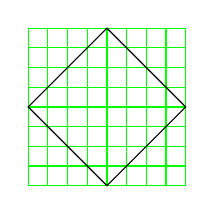
\begin{tikzpicture}
\draw[step=0.25cm,color=green] (-1,-1) grid (1,1);
\draw (1,0) -- (0,1) -- (-1,0) -- (0,-1) -- cycle;
\end{tikzpicture}
\captionof{figure}{You can add a background grid using \texttt{step=0.25cm, color=green} as an option}
\end{centering}


\emphasis{step,color,green,grid,begin,end}
\begin{teXXX}
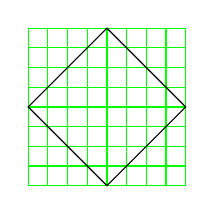
\begin{tikzpicture}
  \draw[step=0.25cm,color=green] (-1,-1) grid (1,1);
  \draw (1,0) -- (0,1) -- (-1,0) -- (0,-1) -- cycle;
\end{tikzpicture}
\end{teXXX}

The grid is specified by providing two diagonally opposing points: (-1,-1)
and (1, 1). The two options supplied give a step size for the grid lines and a
specification for the color of the grid lines, using the \docpkg{xcolor} package

\subsection{Specifying points and paths}

\begin{codeexample}[vbox]

\begin{tikzpicture}
% Define the points of a regular pentagon
\path (0,0) coordinate (origin);
\path (0:1cm) coordinate (P0);
\path (1*72:1cm) coordinate (P1);
\path (2*72:1cm) coordinate (P2);
\path (3*72:1cm) coordinate (P3);
\path (4*72:1cm) coordinate (P4);
% Draw the edges of the pentagon
\draw (P0) -- (P1) -- (P2) -- (P3) -- (P4) -- cycle;
% Add "spokes"
\draw (origin) -- (P0) (origin) -- (P1) (origin) -- (P2)
(origin) -- (P3) (origin) -- (P4);
\end{tikzpicture}
\caption{Drawing a complicated polygon, using paths and the \texttt{draw} command}
\end{codeexample}


Two key ideas used in \tikzname\ are points and paths. Both of these ideas were used
in the diamond examples. Much more is possible, however. For example, points
can be specified in any of the following ways:
\begin{enumerate}
\item  Cartesian coordinates
\item  Polar coordinates
\item  Named points
\item  Relative points
\end{enumerate}

\subsection*{coordinates}
The cartesian coordinates can be defined and named using the following syntax.

%\emphasis{begin,end,coordinate,at,draw}
%\begin{teXXX}
%\begin{tikzpicture}
%  \coordinate (A) at (0,0);
%  \coordinate (B) at (1.25,0.25);
%  \draw[blue] (A) -- (B);
%\end{tikzpicture}
%\end{teXXX}

\noindent This produces:
\begin{tikzpicture}
\coordinate (A) at (0,0);
\coordinate (B) at (1.25,0.25);
\draw[blue] (A) -- (B);
\end{tikzpicture}


We can add labels to the points by using the |label| option.
\begin{tikzpicture}
\coordinate [label=left:\textcolor{orange}{$A$}] (A) at (0,0);
\coordinate [label=right:\textcolor{orange}{$B$}]  (B) at (1.15,0.25);
\draw[blue] (A) -- (B);
\end{tikzpicture}

\emphasis{label,left,label:,right}
\begin{teXXX}
\begin{tikzpicture}
  \coordinate [label=left:\textcolor{orange}{$A$}] (A) at (0,0);
  \coordinate [label=west:\textcolor{orange}{$B$}] (B) at (1.25,0.25);
  \draw[blue] (A) -- (B);
\end{tikzpicture}
\end{teXXX}




If you tempted to write \texttt{label=top:} it will not work, as the command accepts the following keywords.


\begin{tikzpicture}
  \coordinate [label=left:\textcolor{orange}{east}]  (A) at (0,0);
  \coordinate [label=right:\textcolor{orange}{west}] (B) at (0,0);
  \draw[blue] (A)--(B);
\end{tikzpicture}




%To summarize, what we have been doing so far is to learn a set of primitive TikZ commands for drawing paths, drawing shapes and labeling them. All TikZ command work by passing options to them. For example to change the above line to an arrow, we just pass the option |->| to the |draw| command.
%

%\begin{tikzpicture}
%  \coordinate [label=left:\textcolor{orange}{$A$}] (A) at (0,0);
%  \coordinate [label=right:\textcolor{orange}{$B$}] (B) at (1.25,0.25);
%  \draw[->,o-stealth] (A)--(B);
%\end{tikzpicture}
%\caption{Effect of the option \protect\texttt{draw[->]}.}

%\emphasis{begin,end,->,draw}
%\begin{teXXX}
%\begin{tikzpicture}
%  ...
%  ...
%  \draw[->,blue] (A)--(B);
%\end{tikzpicture}
%\end{teXXX}
%
%\section*{Relative coordinates}
%\index{TikZ!coordinates, relative}
%A coordinate can be made "relative" by prefixing it with |++|. relative coordinates are useful in many applications.
%\medskip
%
%\noindent The code is simple, except before the coordinate you add the |++| signs. This tells the PGF engine to add the x,y dimensions of the new coordinate to that of its predecessor's. In many instances this is more intuitive and easier to determine.



%\begin{tikzpicture}
%\draw[step=0.5cm,color=gray] (-1,-1) grid (3.5,3);
%\draw[->,red,thick] (0,0) -- ++(1,0) -- ++(0,1) -- ++(-1,0) -- cycle;
%\draw[->,red,thick] (2,0) -- ++(1,0) -- ++(0,1) -- ++(-1,0) -- cycle;
%\draw[arrows=o-stealth,blue] (1.5,1.5) -- ++(1,0) -- ++(0,1) -- ++(-1,0) -- cycle;
%\end{tikzpicture}
%\caption{Example of use of the \protect\texttt{++} to specify relative coordinates.}
%\label{fig:relative}

%\begin{teXXX}
%\begin{tikzpicture}
%  \draw[step=0.5cm,color=gray] (-1,-1) grid (3.5,3);
%  \draw[red,very thick] (0,0) -- ++(1,0) -- ++(0,1) -- ++(-1,0) -- cycle;
%  \draw[red,very thick] (2,0) -- ++(1,0) -- ++(0,1) -- ++(-1,0) -- cycle;
%  \draw[->,red,very thick] (1.5,1.5) -- ++(1,0) -- ++(0,1) -- ++(-1,0) -- cycle;
%\end{tikzpicture}
%\end{teXXX}
%
%Instead of |++| you can also use a single |+|. This also specifies a relative coordinate, but it does not "update"
%the current point for subsequent usages of relative coordinates. Thus, you can use this notation to specify
%numerous points, all relative to the same "initial" point:
%

%\begin{tikzpicture}
%\draw[step=0.5cm,color=gray] (-1,-1) grid (3.5,3);
%\draw[purple, fill=white] (0,0) -- +(1,0) -- +(1,1) -- +(0,1) -- cycle;
%\draw[purple, fill=white] (2,0) -- +(1,0) -- +(1,1) -- +(0,1) -- cycle;
%\draw[purple, fill=white] (1.5,1.5) -- +(1,0) -- +(1,1) -- +(0,1) -- cycle;
%\path (0,0) node [shape=circle,draw]{(0,0)};
%\end{tikzpicture}
%\caption{Example of use of the \protect\texttt{+} to specify relative coordinates.}
%\label{fig:relative1}

%\begin{teXXX}
%  \draw (0,0) -- +(1,0) -- +(1,1) -- +(0,1) -- cycle;
%  \draw (2,0) -- +(1,0) -- +(1,1) -- +(0,1) -- cycle;
%  \draw (1.5,1.5) -- +(1,0) -- +(1,1) -- +(0,1) -- cycle;
%\end{teXXX}
%
%
%Personally, I don't favour this method of specifying co-ordinates, but it can be useful, if you are automating the production of figures through an external script\sidenote{For drawing Bezier curves, the \texttt{+} behaves differently.  You can refer to the PGF Manual for more details.}.
%
%
%\section*{Arrows}
%\index{TikZ!arrows}
%The function |->| creates a tooltip arrow. You can use different arrow tips and there is a long section for them in the PGF manual. You can even define your own.

\bgroup
%\centering
%\begin{tikzpicture}
%  \draw[->] (0,0) -- (2,0);
%  \draw[arrows=o-stealth,blue] (0,-0.3) -- (2,-0.3);
%  \draw[->,o-stealth,orange] (0,-0.6) -- (2,-0.6);
%  \draw[arrows=|-stealth,purple] (0,-0.9) -- (2,-0.9);
%\end{tikzpicture}
%\captionof{figure}{Special arrow endings}
%\label{fig:specials}
\egroup
%
%\emphasis{o,stealth,begin,end,draw}
%\begin{teXXX}
%\begin{tikzpicture}
% \draw[->] (0,0) -- (2,0);
% \draw[arrows=o-stealth,blue] (0,-0.3) -- (2,-0.3);
% \draw[->,o-stealth,orange] (0,-0.6) -- (2,-0.6);
% \draw[arrows=X-stealth,purple] (0,-0.9) -- (2,-0.9);
%\end{tikzpicture}
%\end{teXXX}

%

\begin{verbatim}

\begin{tikzpicture}
% Define the points of a regular pentagon
\path (0,0) coordinate (origin);
\path (0:1cm) coordinate (P0);
\path (1*72:1cm) coordinate (P1);
\path (2*72:1cm) coordinate (P2);
\path (3*72:1cm) coordinate (P3);
\path (4*72:1cm) coordinate (P4);
% Draw the edges of the pentagon
\draw (P0) -- (P1) -- (P2) -- (P3) -- (P4) -- cycle;
% Add "spokes"
\draw (origin) -- (P0) (origin) -- (P1) (origin) -- (P2)
(origin) -- (P3) (origin) -- (P4);
\end{tikzpicture}
\end{verbatim}





\section{Nodes}

A node is a small part of a picture. When a node is created, you provide a position where the node
should be drawn and a shape. A node of shape circle will be drawn as a |circle|, a node of shape |rectangle|
as a rectangle, and so on. A node may also contain same text, which is why they can used nodes to show text.

Finally, a node can get a name for later reference.



\emphasis{node,shape,draw}
\begin{teXXX}
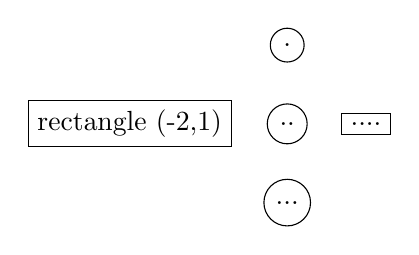
\begin{tikzpicture}
\path ( 0,2) node [shape=circle,draw] {.}
( 0,1) node [shape=circle,draw] {..}
( 0,0) node [shape=circle,draw] {...}
( 1,1) node [shape=rectangle,draw] {....}
(-2,1) node [shape=rectangle,draw] {rectangle (-2,1)};
\end{tikzpicture}
\end{teXXX}
\medskip

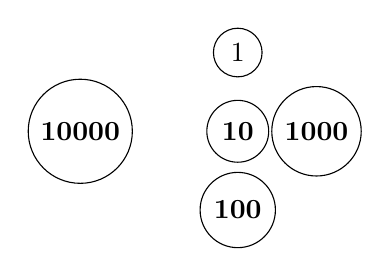
\begin{tikzpicture}
\path ( 0,2) node [shape=circle,draw] {1}
( 0,1) node [shape=circle,draw] {\textbf{10}}
( 0,0) node [shape=circle,draw] {\textbf{100}}
( 1,1) node [shape=circle,draw] {\textbf{1000}}
(-2,1) node [shape=circle,draw] {\textbf{10000}};
\end{tikzpicture}

In the above code, this text is empty (because of the
|empty {}|). So, why do we see anything at all at all the nodes? The answer is the draw option for the node operation: It
causes the |shape| around the text" to be drawn. If you have an empty |{}|, PGF still sees the empty space as a character and justs draws around it. The reason is than TikZ automatically adds some space around the text. The amount is set
using the option |inner sep|. So, to increase the size of the nodes. Modifying the example slightly we get.



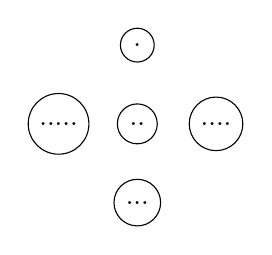
\begin{tikzpicture}
\path ( 0,2) node [shape=circle,draw] {.}
( 0,1) node [shape=circle,draw] {..}
( 0,0) node [shape=circle,draw] {...}
( 1,1) node [shape=circle,draw] {....}
(-1,1) node [shape=circle,draw] {.....};
\end{tikzpicture}

As you can observe the size of the circle has been adjusted to fit the text that is enclosing it. 
Another way to simply add a node is using the |at| syntax:

\begin{texexample}{The node command}{}
\begin{tikzpicture}
\node at (0,0) [circle, draw] {\textbf{100}};
\node at (1,1) [diamond,draw] {\textbf{100}};
\end{tikzpicture}
\end{texexample}

The \cmd{\node} is an abbreviation of the |\path| node. This is a much shorter syntax than |\path| where one would need to add a lot of redundant move-tos  \seepgfmanual{215}.

If you have many nodes another way of achieving the example outlined above is to use the |\draw| command in comination with node and at.

\begin{texexample}{The node command}{}
\begin{tikzpicture}
\tikz \draw[fill=yellow!80!black]
(0,0) node {first node}
-- (1,1) node[draw, behind path] {second node}
-- (0,2) node[fill=red!20,draw,double,rounded corners] {third node};

\node at (0,0) [circle, draw] {\textbf{100}};
\node at (1,1) [diamond,draw]{\textbf{100}};
\end{tikzpicture}
\end{texexample}

\subsection{Drawing shapes}

PGF abd \tikzname\ come with a number of predefined shapes:
\begin{itemize}
\item rectangle
\item circle, and
\item coordinate
\end{itemize}

\begin{centering}

\begin{tikzpicture}
\draw (0,0) circle (1cm);
\draw (0.5,0) circle (0.5cm);
\draw (0,0.5) circle (0.5cm);
\draw (-0.5,0) circle (0.5cm);
\draw (0,-0.5) circle (0.5cm);
\end{tikzpicture}
\captionof{figure}{Drawing multiple circles, using mutiple \texttt{draw} commands}
\end{centering}


A circle is specified by providing its center point and the desired radius. The
command:

\medskip

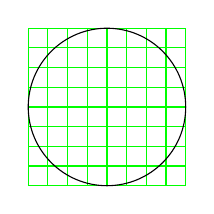
\begin{tikzpicture}
  \draw[step=0.25cm,color=green] (-1,-1) grid (1,1);
  \draw (0,0) circle (1cm);
\end{tikzpicture}
\medskip

\begin{teXXX}
\begin{tikzpicture}
  \draw (x,y) circle (dia);
\end{tikzpicture}
\end{teXXX}



You  can use one |\draw| command to draw multiple circles as shown in \fref{fig:circles}


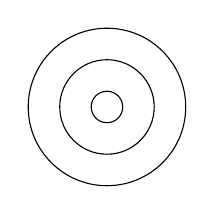
\begin{tikzpicture} 
 \draw (0,0) 
  circle (1cm)
  circle (0.6cm)
  circle (0.2cm)
 ;
\end{tikzpicture}

\emphasis{circle,begin,end}
\begin{teXXX}
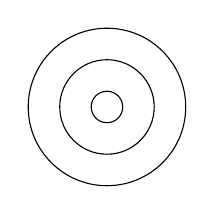
\begin{tikzpicture} 
 \draw (0,0) 
  circle (1cm)
  circle (0.6cm)
  circle (0.2cm)
 ;
\end{tikzpicture}
\end{teXXX}





\begin{center}
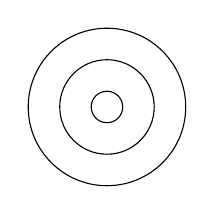
\begin{tikzpicture}
\draw (0,0) circle (1cm)
circle (0.6cm)
circle (0.2cm);
\end{tikzpicture}
\caption{You can use one draw command to draw multiple circles}
\label{fig:circles}
\end{center}
\caption{Drawing multiple circles, using mutiple \texttt{circle} commands}


\subsection{Drawing ellipses}

Ellipses can be drawn in a similar fashion to circles. As an ellipse needs two center points to be specified the command used has the following general form:

\begin{verbatim}
\draw (a,b) ellipse (r1 dim and r2 dim);
\end{verbatim}

We can draw two ellipses as shown in the figure, using the code:
\begin{teX}

\begin{tikzpicture}[scale=0.6]
\draw[color=red] (0,0) ellipse (2cm and 1cm);
\draw[color=red] (0,0) ellipse (1cm and 2cm);
\end{tikzpicture}
\end{teX}

\begin{centering}

\begin{tikzpicture}[scale=0.6]
\draw[color=red] (0,0) ellipse (2cm and 1cm);
\draw[color=red] (0,0) ellipse (1cm and 2cm);
\end{tikzpicture}
\caption[Drawing ellipses]{Use the draw command in combination with ellipse to draw ellipses}
\end{centering}


\begin{teX}
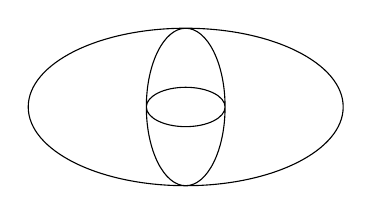
\begin{tikzpicture}
\draw (0,0) ellipse (2cm and 1cm)
ellipse (0.5cm and 1 cm)
ellipse (0.5cm and 0.25cm);
\end{tikzpicture}
\caption{Drawing multiple circles, using mutiple \texttt{draw} commands}
\end{teX}

\section{Drawing more complicated shapes}
we can place a parabola in a rectangle as shown in \fref{fig:parabola}, by using the |rectangle| and the |parabola| options.

\bgroup
\centering

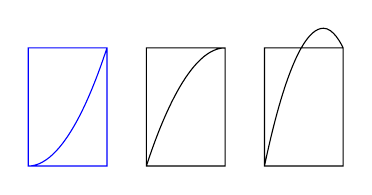
\begin{tikzpicture}
\draw[color=blue] (0,0) rectangle (1,1.5)
(0,0) parabola[color=orange] (1,1.5);
\draw[xshift=1.5cm] (0,0) rectangle (1,1.5)
(0,0) parabola[bend at end] (1,1.5);
\draw[xshift=3cm] (0,0) rectangle (1,1.5)
(0,0) parabola bend (.75,1.75) (1,1.5);
\end{tikzpicture}
\captionof{figure}{Parabolas drawn using the parabola and rectangle options.}
\label{fig:parabola}
\egroup




\emphasis{parabola,rectangle}
\begin{teX}
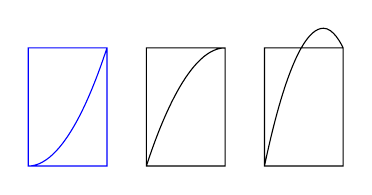
\begin{tikzpicture}
\draw[color=blue] (0,0) rectangle (1,1.5)
(0,0) parabola[color=orange] (1,1.5);
\draw[xshift=1.5cm] (0,0) rectangle (1,1.5)
(0,0) parabola[bend at end] (1,1.5);
\draw[xshift=3cm] (0,0) rectangle (1,1.5)
(0,0) parabola bend (.75,1.75) (1,1.5);
\end{tikzpicture}
\caption{Parabolas drawn using the parabola command}
\label{fig:parabola}
\end{teX}

\subsection*{The shape library}

\begin{tikzpicture}
\draw [help lines] (0,0) grid (2,2);
\draw [blue, dashed] (1,1) circle(1cm);
\draw [red, dashed] (1,1) circle(.5cm);
\node [star, star point height=.5cm, minimum size=2cm, draw]
at (1,1) {S};
\end{tikzpicture}

\section{Iterations}
One convenient construct provided with TikZ is a |foreach| command sequence

\begin{texexample}{Tikz loops}{tz:ex}
\centering
\begin{tikzpicture}[scale=2, color=bgsexy]
\foreach \i in {1,...,4}
{
  \path (\i,0) coordinate (X\i);
  \fill (X\i) circle (1pt);
}
  \foreach \j in {1,...,3}
{
  \path (\j,1) coordinate (Y\j);
  \fill (Y\j) circle (1pt);
}
\foreach \i in {1,...,4}
{
  \foreach \j in {1,...,3}
  {
     \draw[color=bgsexy] (X\i) -- (Y\j);
  }
}
\end{tikzpicture}
\captionof{figure}{Drawing a bi-partite garph using foreach loops}
\end{texexample}



\section{The pgfplots package}



\subsection{Loading data from files}

Scientific work, especially that associated with research tends to generate
a lot of data. The data would normally come from external applications and stored in files. With |TikZ| one can import the data
by using the word |file|:

\emphasis{addplot,file,x}
\begin{teXXX}
 \addplot file {./raw/wavefunctions/wavefunc\x.dat};
\end{teXXX}

In the example we use a file with a path. The data is saved in
files with the same name but a different ending. We use a |foreach| function to add the ending i.e, the file names are |wavefunc1|, |wavefunc2| and |wavefunc3|. By using external data files and the foreach command it can substantially reduce the amount of text in the macros. This improves debugging and readability.

\begin{texexample}[colback=white]{Loading files}{ex:lfiles}
\centering
\begin{tikzpicture}[scale=0.8]
    \begin{axis}[smooth,
    xlabel=$n$,
    ylabel=$\Theta{j}{n}$]
    \foreach \x in {0,...,2}
    {
        \addplot file {./raw/wavefunctions/wavefunc\x.dat};
    }
    \legend{$j=0$,$j=1$,$j=2$};
    \end{axis}
\end{tikzpicture}
\captionof{figure}{Example plot with data imported from external files, using \texttt{file}}
\end{texexample}


\begin{teXXX}
\begin{tikzpicture}[scale=0.6]
  \begin{axis}[
    xlabel=$n$,
    ylabel=$\Theta{j}{n}$]
    \foreach \x in {0,...,2}
    {
      \addplot file {./raw/wavefunctions/wavefunc\x.dat};
    }
    \legend{$j=0$,$j=1$,$j=2$};
  \end{axis}
\end{tikzpicture}
\end{teXXX}



\section*{Plotting functions}
Functions can be defined for plotting using a variety of methods. They are powerful but generally difficult to remember.



\section{Saving Data to a file}

You can save your data to a file in many ways. One easy way is to use
the \docpkg{filecontents} package. This package extends the LaTeX environment
with the same name, but allows you to overwrite the file {\protect\ctan{filecontents}}.

\begin{teXXX}
\documentclass[justified]{tufte-book}
\usepackage{pgfplots,lipsum,booktabs}
\usepackage{pgfplotstable}
\pgfplotsset{compat=newest}
\usepackage{filecontents*}
\begin{filecontents}{my1.dat}
    Label       value       num
    Integrity     33         4
    Standalone    14         3
    Interface      6         2
    Overall       18         1
\end{filecontents*}
\begin{document}
    your code here ...
\end{document}
\end{teXXX}

It is good practice to keep, such data at the top of your file, although with
the |filecontents| package, they can be inserted anywhere. Sometimes it maybe
easier to have a number of minimal files with the type of charts you using regularly and just update the data on top. In general if the data is entered
by hand rather than generated automatically by software this is a good way
to keep your work tidy.

\newenvironment{Chart}[1][black!70!green]{%
%%  defaults
    \gdef\level##1{Level ##1}
    \def\setchartwidth##1{%
      \def\chartwidth{##1}}%
    \setchartwidth{3.9cm}%
    \def\chartcolor{#1}
    \newcommand\addTitle[2][test]{
%% For the chart title we set it in a minipage for
%% better control
    \def\charttitle{\minipage{4cm}%
       \footnotesize %
       \centering\textbf{##2}\\##1%
       \endminipage}}%
   \def\xlabel{Completion (\%)}%
%% renders the chart 
    \def\renderChart{%
%%
    \footnotesize%
%%
%%
    \IfFileExists{#1.dat}{Test}{}
   \begin{tikzpicture}
   \begin{axis}[
    xbar, width=\chartwidth,title=\charttitle,
    y=0.5cm, enlarge y limits={true, abs value=0.75},
    xmin=0, xmax=100,enlarge x limits={upper, value=0.25},
    xlabel=\xlabel,
    %ylabel=Label,
    xmajorgrids=true,
    ytick=data,
    yticklabels from table={\dataTable}{Label},
    nodes near coords, nodes near coords align=horizontal
     ]
    \addplot[draw=none, fill=\chartcolor] table [x=value, y=num]
    {\dataTable};
    \end{axis}%
    \end{tikzpicture}}}
{}

\begin{comment}
\begin{figure*}
\centering

\hskip-2cm\begin{Chart}
 \addTitle[Mechanical Systems]{Shangri-la}
 \def\dataTable{SH-mechanical.dat}
 \renderChart
\end{Chart}\hspace{0.3cm}
\begin{Chart}
 \addTitle[FM-200 System]{All areas}
 \def\dataTable{my1.dat}
 \renderChart
\end{Chart}
\begin{Chart}
 \addTitle[Electrical Works]{Merweb}
 \def\dataTable{my6.dat}
 \renderChart
\end{Chart}
\caption{Mechanical Systems Shangrila. Commissioning status}
\end{figure*}


\begin{filecontents*}{my1.dat}
Label     value       num
Integrity         33            4
Standalone      14            3
Interface        6            2
Overall           18            1
\end{filecontents*}

\begin{filecontents*}{SH-mechanical.dat}
Label     value       num
{Fan coil units}       43             8
{Air Handling Units}       13             7 
{CW Pumps}       13             6
{ECU}       11             5
{Pressurization Fans}        15             4
{Smoke Extract Fan}       5             3
{Jet fan}       5             2
{Overall}       12              1
\end{filecontents*}

\begin{filecontents*}{my6.dat}
Label    value         num   other
{Level 7}  50           11   13
L6         90           10   12
L5       80             9    16
L4       90             8    18
L3       70             7    90
L2       80             6    21
L1       70             5    22
\end{filecontents*}

\begin{filecontents*}{carparkventilation.dat}
Label    value         num   other
L5         50           11   13
L4         90           10   12
L3         80           9    16
GR         90           8    18
B1         70           7    90
B2         80           6    21
B3         70           5    22
\end{filecontents*}
%% CO SYSTEM
%% DATA
\begin{filecontents*}{carparkco.dat}
Label    value         num   other
L5         78           7   13
L4         90           6   12
L3         80           5    16
GR         90           4    18
B1         70           3    90
B2         80           2    21
B3         70           1    22
B5         50          {}    {}
\end{filecontents*}

\begin{filecontents*}{carparkco2.dat}
value,   num,   other,
78,       7,   13,
90,       6,   12,
80,       5,    16,
90,       4,    18,
70,       3,    90,
80,       2,    21,
70,       1,    22,
\end{filecontents*}
\end{comment}






















%\let\luacmd\textbf
\chapter{Presenting Data in Charts and Visualizations}
\label{ch:charts}
\pagestyle{headings}

There can be no doubt that the hallmark of scientific reports and publications is the graphical presentation of the results. Graphs show relationships underlying observations in a way no other device can provide\footnote{\textit{Doing science: design, analysis, and communication of scientific research}
 By Ivan Valiela}.  Charting is both an art and a science. Modern typography on charts and infographics look at Tufte as inspiration.
Tufte advocates to minimize the ink to data ratio and although this is not always possible it is good advice.
In this section we would look at charting in general which is probably of interest to most of the readers
in this book.  Another good source of information is Stephen Few’s website the \href{perpetualedge}{perceptualedge} \footnote{\protect\url{http:\\perceptualedge.com}}  with a number of excellent articles on data visualization. 

\begin{figure}[htbp]
\includegraphics[width=\textwidth]{beautiful-evidence}
\caption{An extract from Tufte’s book \textit{Beautiful Evidence}. In his book Tufte advocates that science and art have in common \emph{intense seeing}, the wide-eyed observing that generates empirical information. \textit{Beautiful Evidence} is about how \emph{seeing} is turned into \emph{showing}. \cite{Tufte2006}}
\end{figure}

\section{Graphical Perception}

When a person looks at a graph, the information is decoded by the person’s visual system. A graphical method is successful only if the decoding is effective. Cleveland \citeyearpar{cleveland1985} in an often quoted study designed experiments and made suggestions as to how graphical data can be improved by selecting representations that have high rank in Table~ref{tbl:cleveland}. Cleveland and McGill at the time employed as statistical scientists at At \& T Bell Laboratories, investigated how we perceive quantitative information and produced a table as to how to order elementary tasks by accuracy. They suggested graphs should exploit tasks as high in the ordering as possible. The tasks are ordered from most accurate to least.

\begin{table}[htbp]
\centering

\begin{tabular}{lp{4.5cm}}
\toprule
Rank  & Position along a common scale\\
\midrule
1  & Position along a common scale\\
2  & Position on identical but nonaligned scales\\
3  & Length\\
4  & Angle\\
    & Slope (with $\theta$ not too close to 0, $\pi/2$, or $\pi$ radians)\\
5   & Area\\
6   &Volume\\
     &Density\\
     &Colour saturation\\
7   & Colour hue\\         
\bottomrule
\end{tabular}
\caption{Rank table for chart visual representation.}
\end{table}



\begin{figure}[htbp]
\includegraphics[width=0.45\textwidth]{length-judgement}
\caption{The top panel is a divided bar chart. This graphical method requires length judgement; for example
to compare and order the values in group A is not easy. In the bottom panel the values are shown by a dot
chart. All values on the graph can be visually compared by judgements of position along a common scale, an
easier task. Now the ordering of the values in group A is easy to perceive. Adapted from \cite{cleveland1985}.}
\end{figure}

\section{How to Draw your Charts}

With the newer engines the limitations of fonts are now part of TeX’s history, so you can use other programs. However, the use of PGF and TikZ or pstricks is still an unbeatable way to produce high quality charts and graphs.
For visualizations other tools might be necessary. Asymptote is on of them and I am sure you have other in your toolbox.

\section{Tufte like charts}

During the last stages of a Project, it maybe easier to visualize the
main areas where effort needs to be exerted by using simple charts. One
such chart is shown in Figure~\ref{fig:tufte-overall}. When this chart
was prepared efforts were made to complete the physical installation
as well as plan and commission the plant. The use of colour in this
chart highlights the commissioning, so one can easily see the expectations. Although the percentages are written on top of the bars,
one need not read them to visualize how difficult is to achieve
100\% completion in a Project. On the other hand commissiong can go
fairly fast and can jump by a large percentage, just by
commissioning a couple of additional ELV systems that have approximately
a 10\% weigh factor.

One can easily fit approximately, six to seven months data on
a portrait chart, changing it around to landscape one can fit
more than a year. Personally I am not very happy with such long
projections as they are more like guesses rather than proper estimates.

One other chart that can be used to visualize progress and is more
commonly found in construction is the infamous S-curve. Now, if
the actual planning is detailed enough and granular enough to be
able to pin-point \textit{continuous} progress then it is
appropriate. using it if you can at least obtain weekly progress
estimates.


\begin{figure}[b]
 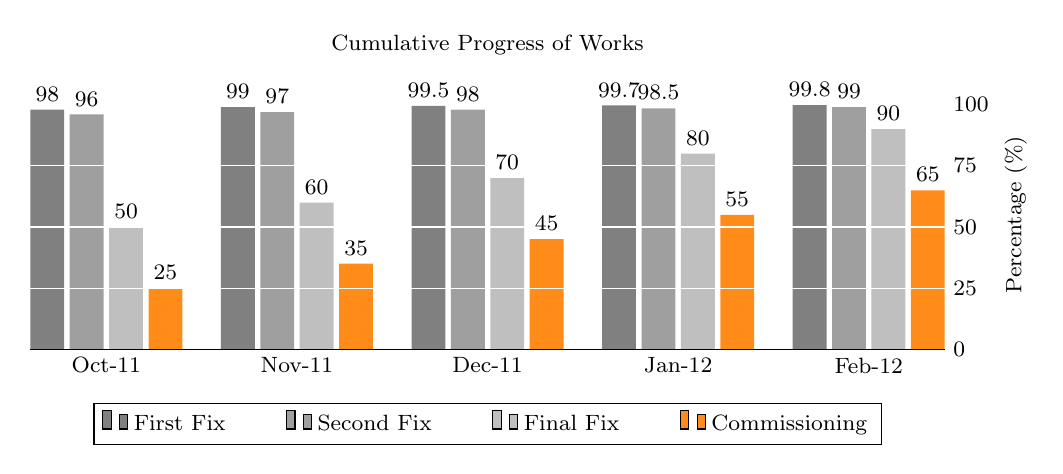
\begin{tikzpicture}
  \footnotesize
  \centering
  \begin{axis}[
        ybar, axis on top,
        title={Cumulative Progress of Works},
        height=5cm, width=13.2cm,
        bar width=0.43cm,
        ymajorgrids, tick align=inside,
        major grid style={draw=white},
        enlarge y limits={value=.1,upper},
        ymin=0, ymax=100,
        axis x line*=bottom,
        axis y line*=right,
        y axis line style={opacity=0},
        ytick={0,25,50,75,100},
        tickwidth=0pt,
        legend style={
            at={(0.5,-0.2)},
            anchor=north,
            legend columns=-1,
            % adds space between the legends
            /tikz/every even column/.append style={column sep=0.7cm}
        },
        ylabel={Percentage (\%)},
        symbolic x coords={
           Sep-11,Oct-11,Nov-11,Dec-11,
           Jan-12,Feb-12,
           Mar-12,
          Apr-12},
       xtick=data,
       nodes near coords={
        \pgfmathprintnumber[precision=2]{\pgfplotspointmeta}
       }
    ]
    \addplot [draw=none, fill=gray] coordinates {
      (Oct-11, 98)
      (Nov-11,99)
      (Dec-11,99.5)
      (Jan-12,99.7)
      (Feb-12,99.8)
       };
   \addplot [draw=none,fill=gray!75!white] coordinates {
      (Oct-11, 96)
      (Nov-11,97)
      (Dec-11,98)
      (Jan-12,98.5)
      (Feb-12,99)
        };
   \addplot [draw=none, fill=gray!50!white] coordinates {
      (Oct-11, 50)
      (Nov-11, 60)
      (Dec-11, 70)
      (Jan-12, 80)
      (Feb-12, 90)
            };
    \addplot [draw=none, fill=orange!90!white] coordinates {
      (Oct-11, 25)
      (Nov-11, 35)
      (Dec-11, 45)
      (Jan-12, 55)
      (Feb-12, 65)
          };
    \legend{First Fix,Second Fix,Final Fix,Commissioning}
  \end{axis}
  \end{tikzpicture}

\caption{\protect\raggedright Cumulative progress for all MEP works. Notice the slower rate of production during the last three months.}
\label{fig:tufte-overall}
\end{figure}


A good graph is uncluttered, clear and focused.

\subsection{Axis Lines}

Most problems with graphs arise from misuse of axes: too heavy, too long, wrong intersection,
ambiquous breaks or too confusing increments and incorrect proportions. An axis is a ruler that established
regular intervals for measuring the information provided. Axes may emphasize, diminish, distort, simplify
or clutter the information.

\clearpage
\begin{multicols}{2}
\subsection{Axis Length}

Graphs should utilize their space around them, as the graph itself is mostly white space. In publications the journal might want to minimize the cost of printing. An axis should not extend beyond the labeled unit od minor tick closest to the last data point.
\columnbreak
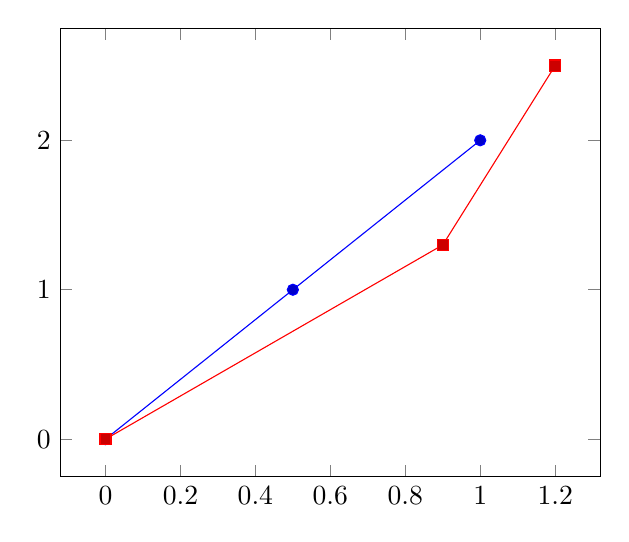
\begin{tikzpicture}
\begin{axis}
\addplot coordinates {
(0,0)
(0.5,1)
(1,2)
};
\addplot coordinates {
(0,0)
(0.9,1.3)
(1.2,2.5)
};
\end{axis}
\end{tikzpicture}
\end{multicols}


\section{The bullet graph}

The bullet graph is considered\footnote{\protect\url{http://www.perceptualedge.com/blog/?p=375}} to be a  better alternative to gauges in dashboards. A solution to a basic chart can be found at tx.se\footnote{\url{http://tex.stackexchange.com/questions/117314/is-there-any-package-to-create-bullet-gauge-graphs}}, by Jake, which sadly in a community of mathematicians, engineers and programmers was not popularized to the extend it deserved. 

Bullet gauges are commonly used to show the current state relative to a reference value with a background that divides the scale into regions.

\begin{figure}[htbp]
\centering

\includegraphics{./images/bullet-graph.png}
\caption{Bullet graph with annotations, indicating the various components of the graph.}
\end{figure}



current sales --
previous sales --
good -- 
great -- last shade box

Formatting: The color is preferable to be a range of distinct hues, which can also assist by those who are colorblind. It is also reproduced better when photocopies.  Intensities are preferred as follows:

three: 40\%, 25\% and 10\%

\makeatletter
\newenvironment {bulletgraph} {\luacode@begin\luacode@table@soft} {}
\makeatother

\pgfplotscreateplotcyclelist{bullet}{
{fill=color1, draw=none},
{fill=color2, draw=none},
{fill=color3, draw=none},
}

\pgfplotsset{mark options/.style={color=black!80}}
\pgfplotsset{barwidth/.style= {bar width=1.2ex} }
\pgfplotsset{chartheight/.style ={height=#1}}

\providecommand{\bulletgauge}[4][]{
    \begin{tikzpicture}[scale=0.8, font=\arial]
    \begin{axis}[
       width=8cm,
       chartheight = 60pt,
      % height=60pt,
       %y=2ex,
       xtick pos=left, 
       xtick = {0,50,...,400, 450},
       ytick=\empty,
       xmin=50, xmax=450,
        %enlarge y limits={abs=0ex},
        tick align=outside,
        axis on top,
        every axis title/.style={
            at={(rel axis cs:0,0.5)},
            anchor=east,
            align=right,
            xshift=-0.5em
        },
        #1
    ]
    \pgfplotsinvokeforeach{#4}{
        \pgfplotsset{cycle list name=bullet}
        \addplot +[xbar, bar width=7ex ] coordinates {(##1,0)};
    }
    \addplot [fill= barcolour, xbar, barwidth ] coordinates {(#2,0)};    
    \addplot [mark=|, mark options={very thick}, mark size=2ex, ] coordinates {(#3,0)}; 
    \end{axis}
    \end{tikzpicture}
}

\begin{scriptexample}{}{}
\begin{bulletgraph}
  m = require("i18n.bulletgraph")
 local data = {
     title = 'Valuation (Jan)',
     ranges = {230,300,500},
     bar = 200,
     marker = 220}
     local options = {
        barcolour = 'red!90'
   } 
m:render(data,options)        
\end{bulletgraph}
\medskip

\begin{bulletgraph}
   m = require("i18n.bulletgraph")
   local data = {
      title = 'Valuation (Apr)',
      ranges = {200,300,500},
      bar = 250,
      marker = 300}
   -- render the plot
   m:render(data,options)           
\end{bulletgraph}
\end{scriptexample}

Use an updated pgfplotsversion as we use |\pgfplotsset{compat=1.11}|, when we load the \pkgname{phd}. The environment |\begin{bulletgraph}|  is a |\luacode|  based environment and hence all the code has to be in lua syntax.

The code load the lua module |bulletgraph| and we the graph is rendered using the method \luacmd{render()}. The method, like most of the plotting routines provided by the package takes two arguments |data| and |options|.

\begin{texexample}{Bullet Plots}{ex:bulletplot}
\begin{bulletgraph}
local  bgraph = require("i18n.bulletgraph")
local data = {
     title = 'Valuation (Jan)',
     ranges = {230,300,500},
     bar = 200,
     marker = 220}
local options = {
        barcolour = 'red!90'
   } 
bgraph:render(data,options)        
\end{bulletgraph}
\end{texexample}

If you are familiar with Javascript you must have come across jQuery and its many plugins. The bulletgraph methods work in a similar fashion, where the options are a set of key values, that are used as a mixin with a set of default key values. If you only want to change the color of the bar, you only specify the color in the options the rest
are inherited from default values. All the \pkgname{phd} package routines, follow this design pattern to simplify the user interface and to enable typographical styles to be maintained throughout a publication. The best way to draw such charts is without the |options|. This separation of the interface, it also separates the data from the presentational aspects of drawing the plots.

\begin{texexample}{Bullet Plots (without options)}{ex:bulletplot1}
\begin{bulletgraph}
local  bgraph = require("i18n.bulletgraph")
local data = {
     title = 'Valuation (Jan)',
     ranges = {230,300,500},
     bar = 200,
     marker = 220}
bgraph:render(data,options)        
\end{bulletgraph}
\end{texexample}

\section{Using matplotlib}

Many researchers use Python to produce charts. A good guide can be found at \href{https://github.com/jbmouret/matplotlib_for_papers}{jbmournet} at github. There was also a good discussion at HN\footnote{\protect\url{https://news.ycombinator.com/item?id=9043571}}.












%\let\sidenote\footnote
\chapter{How to Develop your Own Class or Package}

\cxset {epigraph width=0.67\textwidth}

\epigraph{First there was one user and I took a lot of time to satisfy myself. Then I had 10 users, and a whole new level of difficulties arose. Then I had a hundred users and another level of things happened. I had a thousand users, I had ten thousand each of those were special phases in the development, important. I couldn't have gone with ten thousand until I'd done
it with a thousand. But each time a new wave of
changes came along, the idea was to have \tex get
better, and not get more diverse as it needed to handle
new things.}{Donald Knuth}

\parindent1em

\section{Introduction}


To \emph{make} a book is an interesting and somewhat involved process \cite{town}. The text is set in type and printed on pages, the pages are gathered and folded into signatures and these are gathered and folded into signatures and these are then bound and covered. Many of the aspects of this process that has passed down to us by previous generations is discussed extensively in other sections of this book.  Class authors have to distill this knowledge in a set of typographical rules to be described in a class file. The first thing such an author must do is to describe the \emph{rationale} of developing such a class. The |octavo| \citep{octavo} class was developed to enable printing books in dimensions that follow traditional styles. The \citep{memoir}  class to offer a flexible system on which other classes could be based and so does \citep{koma}. The |tufte-book| and |tufte-handout| classes to provide a style that resembles those found in Tufte books. Many Universities offer \emph{Thesis} classes to standardize the way these are produced. Many of these Universities, translated the styles previously typed and the results are a typographical disaster, only mitigated by the ability to display beautiful mathematics. As these are printed on standard \emph{photocopy paper} one cannot do much with the layout. 

\section{Identifying your class}

The first thing a class must do is to identify any other formats it needs and to announce
its name. This is accomplished using the two commands 
\docAuxCommand{NeedsTeXFormat} and \docAuxCommand{ProvidesClass}.

The following example, delares the version of \LaTeXe\ that it requires and then
gives the class name. It can be found in the preable of most well written classes. You should also put some remarks to identify you as the author, the version number and other similar details. These are discussed in more detail in the next Chapter, where you will see how to automate documentation for your class.

\begin{teX}
\NeedsTeXFormat{LaTeX2e}[1994/06/01]
\ProvidesClass{myclass-book}[2010/12/11 v3.5.0 myclass-book]
\end{teX}

The above syntax must be followed exactly so that this information can be
used by \texttt{LoadClass} or \texttt{documentclass} (for classes) or \docAuxCommand{RequirePackage}
 or\cmd{usepackage} (for packages) to test that the release is not too old.
The whole of this $<release-info>$ information is displayed by \docAuxCommand{listfiles} and
should therefore not be too long.

\begin{teX}
%%
% Load the common style elements
\input{myclass-common.def}
\end{teX}


Another command that can be used is \docAuxCommand{ProvidesFile}. 
This is similar to the two previous commands except that here the fullname,
including the extension, must be given. It is used for declaring any files other
than main class and package files.

This is useful, if you decide to have your main definitions in a separate file.



\section{Class Options}

Before we see in detail how to add options to a class, we need to review a package called
\pkgname{xkeyval}. Unless you are in the business of re-discovering wheels, this is an absolute must
for developing, readable and maintenable code and your class is to provide many options. 
\begin{teX}
\usepackage[textcolor=red,font=times]{mypack}
\end{teX}

Class options are best set by using booleans\cmd{newboolean}.

We first set a new boolean that we |name@myclass@afourpaper.| This is used using the package
\texttt{ifthen}\sidenote{The ifthen package was developed by 
David Carlisle, can be downloaded at \url{ http://www.ifi.uio.no/it/latex-links/ifthen.pdf }} 
Then we can |DecalareOptionX| and we set the boolean to default to true. If the user then types

myclass[a4paper]

The a4paper options will be set. This is a much better and concise way of defining options.
\cmd{newboolean}


\begin{teX}
\newboolean{@myclass@afourpaper}
\DeclareOptionX[myclass]<common>{a4paper}
  {
   \setboolean{@myclass@afourpaper}
   {true}
  }
\end{teX}
\medskip

Note that the command provide by \texttt{ifthen} \docAuxCommand{setboolean} takes true or false, as \#2, and sets \#1 accordingly. In the above code we set the option as true. 


It is much easier and most programmers use the \texttt{ifthen} package to check
for option booleans

\begin{teX}
\ifthenelse{\boolean{@myclass@afourpaper}}
  {\geometry{
        a4paper,
        left=24.8mm,
        top=27.4mm,
        headsep=2\baselineskip,
        textwidth=107mm,
        marginparsep=8.2mm,
        marginparwidth=49.4mm,
        textheight=49\baselineskip,
        headheight=\baselineskip
    }
  }
 {}
\end{teX}

\section{Set-up the font sizes}

LaTeX does not provide definitions of all the font-sizes. Unless you are
extending an existing class, this is one of the first tasks you need to 
do in your new class.

Normally class authors will define all the commonly defined size commands,
such as  \cmd{small}, \cmd{normalsize} and other similar commands.

In the example shown below, we first start by defining the \cmd{normalsize} font
size. In this book the \cmd{\normalsize}  is defined as 14pt. We also define the vertical
spaces that we need to have abovedisplay and belowdisplayskip. These are all very difficult to
remember and once you have something you are happy with, just copy from class to class
or even define a samll definition file to keep them all together.


{\fontfamily{phv}\selectfont Helvetica looks like this}
and {\fontencoding{OT1}\fontfamily{ppl} Palatino looks like this}.


 The user has access to a number of commands which change the size of
 the fount, relative to the `main' size used for the bulk of the text.


 These \cmd{size} commands issue a \cmd{@setfontsize}\index{Latex kernel!@setfontsize} 
 command.

\begin{teX}
  \@setfontsize\size\font-size{baselineskip} where:
\end{teX}



  \begin{description}
    \item {font-size} The absolute size of the fount to use from
        now on.
    \item{baselineskip} The normal value of \cmd{baselineskip}
        for the size of the fount selected. (The actual value will be
       % |\baselinestretch| * \meta{baselineskip}.)
    \end{description}

A number of commands, defined in the \LaTeX  kernel, shorten the
following  definitions and are used throughout. These are:

    \begin{center}
    \begin{tabular}{ll@{\qquad}ll@{\qquad}ll}
    \verb=\@vpt= & 5 & \verb=\@vipt= & 6 & \verb=\@viipt= & 7 \\
    \verb=\@viiipt= & 8 & \verb=\@ixpt= & 9 & \verb=\@xpt= & 10 \\
    \verb=\@xipt= & 10.95 & \verb=\@xiipt= & 12 & \verb=\@xivpt= & 14.4\\
    \ldots
    \end{tabular}
    \end{center}


\subsection{Setting up the normalsize}
 The user command to obtain the `main' size is \cmd{normalsize}. \LaTeX\
 uses \cmd{@normalsize} \index{Latex kernel!@normalsize} when referring to the main size and maintains this
 value even if \doccmd{normalsize} is redefined. The \doccmd{normalsize} macro also
  sets values for \cmd{abovedisplayskip}, \cmd{abovedisplayshortskip} and 
\cmd{belowdisplayshortskip}.



\begin{teXXX}
%%
% Set the font sizes and baselines to match Tufte's books
% normalsize
%%
\renewcommand\normalsize{%
   \@setfontsize\normalsize\@xpt{14}%
   \abovedisplayskip 10\p@ \@plus2\p@ \@minus5\p@
   \abovedisplayshortskip \z@ \@plus3\p@
   \belowdisplayshortskip 6\p@ \@plus3\p@ \@minus3\p@
   \belowdisplayskip \abovedisplayskip
   \let\@listi\@listI}

\normalbaselineskip=14pt
\normalsize
\end{teXXX}



\begin{teXXX}
\renewcommand\small{%
   \@setfontsize\small\@ixpt{12}%
   \abovedisplayskip 8.5\p@ \@plus3\p@ \@minus4\p@
   \abovedisplayshortskip \z@ \@plus2\p@
   \belowdisplayshortskip 4\p@ \@plus2\p@ \@minus2\p@
   \def\@listi{\leftmargin\leftmargini
               \topsep 4\p@ \@plus2\p@ \@minus2\p@
               \parsep 2\p@ \@plus\p@ \@minus\p@
               \itemsep \parsep}%
   \belowdisplayskip \abovedisplayskip
}
\renewcommand\footnotesize{%
   \@setfontsize\footnotesize\@viiipt{10}%
   \abovedisplayskip 6\p@ \@plus2\p@ \@minus4\p@
   \abovedisplayshortskip \z@ \@plus\p@
   \belowdisplayshortskip 3\p@ \@plus\p@ \@minus2\p@
   \def\@listi{\leftmargin\leftmargini
               \topsep 3\p@ \@plus\p@ \@minus\p@
               \parsep 2\p@ \@plus\p@ \@minus\p@
               \itemsep \parsep}%
   \belowdisplayskip \abovedisplayskip
}
\renewcommand\scriptsize{\@setfontsize\scriptsize\@viipt\@viiipt}
\renewcommand\tiny{\@setfontsize\tiny\@vpt\@vipt}
\renewcommand\large{\@setfontsize\large\@xipt{15}}
\renewcommand\Large{\@setfontsize\Large\@xiipt{16}}
\renewcommand\LARGE{\@setfontsize\LARGE\@xivpt{18}}
\renewcommand\huge{\@setfontsize\huge\@xxpt{30}}
\renewcommand\Huge{\@setfontsize\Huge{24}{36}}

%% Define a HUGE for fun
\newcommand\HUGE{\@setfontsize\Huge{38}{47}}  
\end{teXXX}


\section{Adjusting paragraph parameters}

 The parameters which control \TeX 's behaviour when typesetting
 paragraphs receive a bit of a tweak here. Contrary to the usual
 behaviour of modifying the grid with glue when difficulties are
 encountered with vertical space, here we shall try to counteract
 these tendencies and enforce as much as possible uniformity of the 
 grid of lines.

A good value for paragraph indentation is \texttt{parindent 0.5pt}, for vertical spacing between
paragraphs that are indented use 0pt. At this point if you are using any marginals it is a good idea
to allow hyphenation with the \docpkg{ragged2e} package. Since marginals use very narrow paragraphs you may
get a very funny looking marginal text. Using the package, adjustments can be made to hyphenate
the marginal text.

\begin{teXXX}
%%
% \RaggedRight allows hyphenation

\RequirePackage{ragged2e}
\setlength{\RaggedRightRightskip}{\z@ plus 0.08\hsize}
\setlength{\RaggedRightParindent}{1pc}

% Paragraph indentation and separation for normal text
\newcommand{\@tufte@reset@par}{%
  \setlength{\RaggedRightParindent}{1.0pc}%
  \setlength{\parindent}{1pc}%
  \setlength{\parskip}{0pt}%
}
\@tufte@reset@par

% Paragraph indentation and separation for marginal text
\newcommand{\@tufte@margin@par}{%
  \setlength{\RaggedRightParindent}{0.5pc}%
  \setlength{\parindent}{0.5pc}%
  \setlength{\parskip}{0pt}%
}
\end{teXXX}


\section{Formatting Chapters and Sections}
The section on Chapters etc, has more on this, but we will touch on it briefly.
Most recent class developerss use the \pkgname{titlesec} and \pkgname{titletoc} package to handle the complexity 
of these commands. With the |phd| package this is unecessary. 

\begin{teXXX}
\titleformat{\subsection}%
  [hang]% shape
  {\normalfont\large}% format applied to label+text removed \itshape
  {\thesubsection}% label
  {1em}% horizontal separation between label and title body
  {}% before the title body
  []% after the title body
\end{teXXX}

These are normally followed by the ``titlespacing" commands to define the space around these sections.

\begin{teXXX}
%% We set the titlespacing using the package titlesec and titletoc
%
\titlespacing*{\chapter}{0pt}{20pt}{40pt}
\titlespacing*{\section}{0pt}{3.5ex plus 1ex minus .2ex}{2.3ex plus .2ex}
\titlespacing*{\subsection}{0pt}{3.25ex plus 1ex minus .2ex}{1.5ex plus.2ex}
\end{teXXX}

\section{Adjusting the Index}

For classes representing books, the index is treated like a chapter whereas for others it is normally
treated like a section. Whatever your document ends up like, indices are best done in a multi-column environment.
One possibility is shown below, using the package "multcol".

\begin{teXXX}
\RequirePackage{multicol}
\renewenvironment{theindex}
  {\begin{fullwidth}%
    \small%
    \ifthenelse{\equal{\@tufte@class}{book}}%
      {\chapter{\indexname}}%
      {\section*{\indexname}}%
    \parskip0pt%
    \parindent0pt%
    \let\item\@idxitem%
    \begin{multicols}{3}%
  }
  {\end{multicols}%
    
\renewcommand\@idxitem{\par\hangindent 2em}
\renewcommand\subitem{\par\hangindent 3em\hspace*{1em}}
\renewcommand\subsubitem{
    \par\hangindent 4em\hspace*{2em}
}
\renewcommand\indexspace{
    \par\addvspace{
       1.0\baselineskip plus 0.5ex minus 0.2ex}\relax
    }%
%we now  swallow the letter heading in the index
\newcommand{\lettergroup}[1]{}

\end{teXXX}

The code, renews the "theindex" environment, with minor tweaks and defines it as a three column
layout at "fullwidth".

\section{Provide some hooks}
It is useful at the end of the class to allow for localization of the class
by importing a local file. This is easily achieved by checking if the file exists
and then loading it.  If there is a |myclass-book-local.sty|  file, load it.

\begin{teX}
\IfFileExists{myclass-book-local.tex}
  {input{myclass-book-local}
   \MyClassInfoNL{Loading myclass-book-local.tex}}
  {}
\end{teX}

If you intent to publish your class, you may also want to consider adding a hook for a patch-file.


\section{The final act of kindness to your users}
Many common classes, such as the |memoir| use such a tactic to avoid breaking old code.\index{IfFileExists}

\begin{teX}
 \IfFileExists{mypatch.sty}{%
 \RequirePackage{mempatch}}{}
\end{teX}



\chapter{How to Package Your Class}

\cite{pakin2004} 
In the previous chapter we have outlined the main sections that you probably need
to define in your class. In this chapter we will go over the packaging of the class
and automating the generation of user documentation.

\parindent1em

You should also be
familiar with ``LATEX2'' for Class and Package Writers”, which is available
from CTAN (\url{http://www.ctan.org}) and comes with most LATEX2" distributions
in a file called clsguide.dvi. Finally, you should know how to
install packages that are shipped as a \texttt{.dtx} file plus a \texttt{.ins} file.

style (.sty) file is primarily a collection of macro and
environment definitions. One or more style files (e.g., a main style file that
\cmd{input}  or \cmd{RequirePackages} multiple helper files) is called a package.
Packages are loaded into a document with \cmd{usepackage}{hmain .sty filei}.
In the rest of this document, we use the notation texttt{<package>} to represent
the name of your package.

Motivation The important parts of a package are the code, the documentation
of the code, and the user documentation. Using the \docpkg{Doc}  and
DocStrip programs, it’s possible to combine all three of these into a single,
documented LATEX(.dtx) file. The primary advantage of a .dtx file is that
it enables you to use arbitrary LATEX constructs to comment your code.
Hence, macros, environments, code stanzas, variables, and so forth can be
explained using tables, figures, mathematics, and font changes. Code can
be organized into sections using LATEX’s sectioning commands. Doc even
facilitates generating a unified index that indexes both macro definitions (in
the LATEX code) and macro descriptions (in the user documentation). 

This emphasis on writing verbose, nicely typeset comments for code—essentially
treating a program as a book that describes a set of algorithms—is known
as literate programming \cite{literate} and has been in use since the early days of \tex\ .

Furthermore,
this tutorial shows how to write a single file that serves as both documentation
and driver file, which is a more typical usage of the \texttt{Doc} system than
using separate files.

\subsection{The .ins file}

The first step in preparing a package for distribution is to write an installer
(|.ins|) file. An installer file extracts the code from a |.dtx| file, uses \cs{DocStrip}
to strip off the comments and documentation, and outputs a .sty file. The
good news is that a .ins file is typically fairly short and doesn’t change
significantly from one package to another.

\noindent|ins| files usually start with comments specifying the copyright and license
information:


\begin{teXXX}
%%
%% Copyright (C) year by your name %%
%% This file may be distributed and/or modified under the
%% conditions of the LaTeX Project Public License, either
%% version 1.2 of this license or (at your option) any later
%% version. The latest version of this license is in:
%%
%% http://www.latex-project.org/lppl.txt
%%
%% and version 1.2 or later is part of all distributions of
%% LaTeX version 1999/12/01 or later.
%%

\end{teXXX}

The LATEX Project Public License (LPPL) is the license under which most
packages—and LATEX itself—are distributed. Of course, you can release your
package under any license you want; the LPPL is merely the most common
license for LATEX packages. The LPPL specifies that a user can do whatever
he wants with your package—including sell it and give you nothing in return.
The only restrictions are that he must give you credit for your work, and
he must change the name of the package if he modifies anything to avoid
versioning confusion.
The next step is to load DocStrip:

\begin{teXXX}
%%\input docstrip.tex
%%\keepsilent
\end{teXXX}



By default, DocStrip gives a line-by-line account of its activity. These messages
aren’t terribly useful, so most people turn them off:

\begin{teXXX}
\keepsilent
\end{teXXX}

A system administrator can specify the base directory under which all
TEX-related files should be installed, e.g., \texttt{/usr/share/texmf}. (See
\cmd{\BaseDirectory} in the DocStrip manual.) The |ins| file specifies where
its files should be installed relative to that. The following is typical:

\begin{teXXX}
\usedir{tex/latex/packagename}
\preamble
htexti \endpreamble
\end{teXXX}



The next step is to specify a preamble, which is a block of commentary that
will be written to the top of every generated file:

\begin{teXXX}
\preamble

This is a generated file.
Copyright (C) <year> by <your name>
This file may be distributed and/or modified under the
conditions of the LaTeX Project Public License, either
version 1.2 of this license or (at your option) any later
version. The latest version of this license is in:
http://www.latex-project.org/lppl.txt
and version 1.2 or later is part of all distributions of
LaTeX version 1999/12/01 or later.

\endpreamble
\end{teXXX}


The preceding preamble would cause package.sty  to begin as follows:

\begin{teXXX}
%%
%% This is file ‘hpackagei.sty’,
%% generated with the docstrip utility.
%%
%% The original source files were:
%%
%% hpackagei.dtx (with options: ‘package’)
%%
%% This is a generated file.
%%
%% Copyright (C) hyeari by hyour namei %%
%% This file may be distributed and/or modified under the
%% conditions of the LaTeX Project Public License, either
%% version 1.2 of this license or (at your option) any later
%% version. The latest version of this license is in:
%%
%% http://www.latex-project.org/lppl.txt
%%
%% and version 1.2 or later is part of all distributions of
%% LaTeX version 1999/12/01 or later.
\end{teXXX}


\begin{teXXX}
\generate {\file {hstyle-filei} {\from {hdtx-filei} {htagi}}}
\end{teXXX}

We now reach the most important part of a .ins file: the specification of
what files to generate from the |.dtx| file. The following tells DocStrip to
generate hpackagei.sty from hpackagei.dtx by extracting only those parts
marked as `package'  in the .dtx file. (Marking parts of a .dtx file is
described in Section 3.)

\begin{teXXX}
\generate{\file{<package>.sty}{\from{<package>.dtx}{package}}}
\end{teXXX}

\cmd{\generate} can extract any number of files from a given .dtx file. It can
even extract a single file from multiple |.dtx| files. See the DocStrip manual
for details.

\subsection{Generating messages} 

The next part of a |.ins| file consists of commands to output a message to
the user, telling him what files need to be installed and reminding him how
to produce the user documentation. The following set of \cmd{Msg} commands is
typical:

\begin{teXXX}
\obeyspaces
\Msg{****************************************************}
\Msg{* *}
\Msg{* To finish the installation you have to move the *}
\Msg{* following file into a directory searched by TeX: *}
\Msg{* *}
\Msg{* hpackagei.sty *}
\Msg{* *}
\Msg{* To produce the documentation run the file *}
\Msg{* hpackagei.dtx through LaTeX. *}
\Msg{* *}
\Msg{* Happy TeXing! *}
\Msg{* *}
\Msg{****************************************************}
Note the use of \obeyspaces to inhibit TEX from collapsing multiple spaces
into one.
\endbatchfile
Finally, we tell DocStrip that we’ve reached the end of the .ins file:
\endbatchfile
\end{teXXX}


Appendix A.1 lists a complete, skeleton .ins file. Appendix A.2 is similar
but contains slight modifications intended to produce a class (|.cls|) file
instead of a style (|.sty|) file

\section{The .dtx file}
A |dtx|\ file contains both the commented source code and the user documentation
for the package. Running a |dtx|  file through latex typesets the
user documentation, which usually also includes a nicely typeset version of
the commented source code.

Due to some Doc trickery, a |dtx|  file is actually evaluated twice. The first
time, only a small piece of \latex\  driver code is evaluated. The second time,
comments in the |dtx|  file are evaluated, as if there were no `\%'  preceding
them. This can lead to a good deal of confusion when writing |dtx|  files
and occasionally leads to some awkward constructions. Fortunately, once
the basic structure of a |dtx|  file is in place, filling in the code is fairly
straightforward.

\begin{teXXX}
\CharacterTable {<text>}
\end{teXXX}

The second mechanism that Doc uses to ensure that a |dtx|  file is uncorrupted
is a character table. If you put the following command verbatim into
your |dtx|  file, then Doc will ensure that no unexpected character translation
took place in transport:

\begin{teXXX}
% \CharacterTable
% {Upper-case \A\B\C\D\E\F\G\H\I\J\K\L\M\N\O\P\Q\R\S\T\U\V\W\X\Y\Z
% Lower-case \a\b\c\d\e\f\g\h\i\j\k\l\m\n\o\p\q\r\s\t\u\v\w\x\y\z
% Digits \0\1\2\3\4\5\6\7\8\9
% Exclamation \! Double quote \" Hash (number) \#
% Dollar \$ Percent \% Ampersand \&
% Acute accent \’ Left paren \( Right paren \)
% Asterisk \* Plus \+ Comma \,
% Minus \- Point \. Solidus \/
% Colon \: Semicolon \; Less than \<
% Equals \= Greater than \> Question mark \?
% Commercial at \@ Left bracket \[ Backslash \\
% Right bracket \] Circumflex \^ Underscore \_
% Grave accent \‘ Left brace \{ Vertical bar \|
% Right brace \} Tilde \~}
A success message looks like this:
***************************
* Character table correct *
***************************

and an error message looks like this:
! Package doc Error: Character table corrupted.
\end{teXXX}



\subsection{DoNotIndex}



When producing an index, Doc normally indexes every control sequence
(i.e., backslashed word or symbol) in the code. The problem with this level
of automation is that many control sequences are uninteresting from the
perspective of understanding the code. For example, a reader probably
doesn’t want to see every location where \cs{if} is used—or \cs{the} or \cs{let} or
\cs{begin} or any of numerous other control sequences.

As its name implies, the \cs{DoNotIndex} command gives |Doc| a list of control
sequences that should not be indexed. \cs{DoNotIndex} can be used any
number of times, and it accepts any number of control sequence names per
invocation:




\begin{teXXX}
   % \DoNotIndex{\#,\$,\%,\&,\@,\\,\{,\},\^,\_,\~,\ }
   % \DoNotIndex{\@ne}
   % \DoNotIndex{\advance,\begingroup,\catcode,\closein}
   % \DoNotIndex{\closeout,\day,\def,\edef,\else,\empty,\endgroup}
\end{teXXX}




\subsection{User documentation}

We can finally start writing the user documentation. A typical beginning
looks like this:

\begin{teXXX}
% \title{The \textsf{hpackagei} package\thanks{This document
% corresponds to \textsf{hpackagei}~\fileversion,
% dated~\filedate.}}
% \author{hyour namei \\ \texttt{hyour e-mail addressi}}
%
% \maketitle
\end{teXXX}


The title can certainly be more creative, but note that it’s common for
package names to be typeset with \docAuxCommand{textsf} and for \docAuxCommand{thanks} to be used to
specify the package version and date. This yields one of the advantages
of literate programming: Whenever you change the package version (the
optional second argument to \docAuxCommand{ProvidesPackage}), the user documentation
is updated accordingly. Of course, you still have to ensure manually that
the user documentation accurately describes the updated package.

Write the user documentation as you would any \latexe document, except
that you have to precede each line with a |\%|. Note that the |ltxdoc| document
class is derived from article, so the top-level sectioning command is
|\section|, not |\chapter|.



\section{General tips}

Evaluate, if there is a class that is nearer to what you wish to achive. If not do a set of
requirements.

Book structure - start with book or |Octavo| if you need to hack extensively. If not use memoir, |koma| or |tufte-book|.

Paragraph looks

Lists

Figures

Bibliography and citations

Footnotes

Index

Titel pages

Book Cover

Language support

Mathematics

Graphs and figures

Typography - fonts, indentations fontsize etc

headers and footers


\section{Declaring Options}

Most classes or packages will have a good deal of options. These are declared using the
\docAuxCmd{DeclareOption} command. In this part no package loading should take place.

\begin{docCmd} {DeclareOption} { \marg{option} \marg{code}}
  The argument option is the name of the option being declared and the \marg{code} is the
  code that will execute if this option is requested.
\end{docCmd}


\begin{docCmd}{DeclareOption*} { \marg{code}}
  The argument \meta{code} in the star version of the command specifies the action to be 
  taken if an unknown option is specified. Within this argument the \docAuxCmd{CurrentOption}
  refers to the name of the option in question. 
  
\end{docCmd}

For example one could pass all such options
  to another package, using:
  \begin{verbatim}
  \DeclareOption*{\PassOptionsToPackage{\CurrentOption}{A}}
  \end{verbatim}


\section{Executing Options}

Normally after the options have been defined, one would need to provide default values and 
the options need to be executed. 

\begin{docCmd} {ExecuteOptions} { \marg{option list}}
  
\end{docCmd}

You can also |\ExecuteOptions| when declaring other options. There is one caveat. This command
can only be executed prior to executing the |\ProcessOptions| command because, as one of
its last actions, the latter command reclaims all of the memory taken up by the code for
the declared options.

\begin{docCmd} {ProcessOptions*} {}
\end{docCmd}

For some packages it is preferable or essential to process options in the order they
appear in the |usepackage| commands rather than using the order given through the
sequence of the \refCmd{DeclareOption} commands. In this case it one has to use
the star version of the command, i.e, |\ProcessOptions*| rather than |\ProcessOptions|.

\section{Special Commands for class files}

It is sometimes preferable to define a new class based on another and hence to extend it.
To support this concept the \latexe kernel provides two commands, \docAuxCmd{LoadClass} and
\docAuxCmd{PassOptionsToClass}. These two commands can then be used to develop a new class, by adding and extending the functionality of the loaded class.

\begin{docCmd} {LoadClass}{ \oarg{option list}\marg{class}\oarg{release}}
  
\end{docCmd}

For example the |ltxdoc| class loads the standard |article| class. The tufte-book class loads
the |book| class and perhaps the best way to understand the concepts discussed here is to
study these classes.

\section{A minimal class}

\begin{texexample}{Model Class}{ex:modelclass}

\begin{filecontents}{phdexampleclass.cls}
\NeedsTeXFormat{LaTeX2e}
\ProvidesClass{phdexampleclass}[2015/07/07]
\renewcommand\normalsize{\fontsize{}{10pt}{12pt}\selectfont}
\setlength\textwidth{6.5in}
\setlength\textheight{Sin}
\pagenumbering{arabic}
\end{filecontents}

\end{texexample}






















%\input{./sections/acronyms}
%\parindent1em

\chapter{Boxes and glue in TeX}

\setlength{\columnsep}{2em}
{\it Once you understand \tex\rq{}s concept of glue, you may well decide that
it was misnamed; real glue doesn't stretch or shrink in such ways, nor does it
contribute much space between boxes that it welds together. Another word like
\emph{spring} would be much closer to the essential idea, since springs have a natural
width, and since different springs compress and expand at different rates
under tension. But whenever the author has suggested changing \tex's terminology,
numerous people have said that they like the word \emph{glue} in spite of its
inappropriateness; so the original name has stuck. }
\smallskip

{\hfill  ---  Donald E. Knuth}

\medskip   


\parindent1em




\newthought{Traditional typesetting} was a task that depended on assembling the types and inserting them one by one on holding frames. In a way it was an assembly of boxes.
The \tex typesetting system uses a similar model of boxes to typeset content but in addition it also uses the concept of glue to stretch or shrink the text so that it will look better typographically. Boxes contain
typeset objects, such as text, mathematical displays, and pictures, and glue
is flexible space that can stretch and/or shrink by amounts that are under
user control.

\begin{figure}[h]
\centering
\hbox{\drawfontbox{Qwerty}\drawfontbox{fjord}}
\caption{Everything is boxes.}
\end{figure}

\printfontparams

\section*{Boxes}

Boxes in \tex have  a rectangular shape but have
three associated measurements called \emph{height}, \emph{width}, and \emph{depth}.
Figure \ref{fig:boxes} shows a 
picture of a typical box, showing its so-called \emph{reference point} and \emph{baseline}

The reason that they have three dimensions is that a character of text has normally three dimensions as shown in figure \ref{fig:boxes}. As characters need to be lined on a baseline, the depth provides a datum point on which they can be aligned and the depth provides a measure of the portion of the character that is below the baseline.


Boxes and glue are the main tools of \tex. The box can hold text and other items. Glue is simply spacing. It can be horizontal or veritcal spacing, and it can be made as rigid or as flexible as desired.



\begin{minipage}{\linewidth}
\textbf{One important feature of \tex is that it has no knowledge of the shape of the characters it typesets, just the dimensions of each character box.}
\end{minipage}
\medskip

When \tex is typesetting, it is normally in horizontal mode, such as while
it is working on this paragraph. Otherwise, \tex can be in vertical mode, or
in math mode, or three others described in Chapter 13 of The \texbook.
Two low-level TEX commands for boxes are \cmd{hbox}, for a horizontal box,
and \cmd{vbox} for a box in vertical mode. In the latter, \tex is normally still
collecting material for display from right to left: it is not building up a
column of text, as in classical Chinese writing.

In both kinds of boxes, the result is an unbreakable object that acts
much like a single character. \tex reads input as a string of characters,
then breaks that string up in words, each of which forms a box. 
\emph{Word boxes}\index{word boxes}
are then collected into lines, lines into paragraphs, and paragraphs into a
page galley. The space between the words can be normal \emph{interword space},
or \emph{sentence-ending} space, which is somewhat larger in English-language
typesetting, and the space is normally glue, rather than of fixed size.

\tex has a sophisticated mathematical algorithm for figuring out the
best way to stretch or shrink interbox glue to optimize the appearance of
lines and paragraphs. Every so often, \tex checks to see whether it has
enough material saved on the growing page galley to fill a complete output
page, and it asynchronously (and effectively, unpredictably) calls the
output routine whose job it is to figure out where the page break should
happen, ship out a completed page to the |DVI|  file, and replace the galley by
whatever is left over.

In traditional \tex you  can force a line break with the carriage-return command \docAuxCommand{cr},
and a page break with the command \docAuxCommand{eject}, but \tex is an expert system,
and normally handles line and page breaking on its own. \latex provides its own commands such as \cmd{\clearpage} and \cmd{\newpage} and so do all other \tex based formats and systems.

\latex does not modify any of \tex's algorithms but simply it is a set of implemenation
macros.

\section{Units of measurement in TEX}

\tex allows you to specify sizes of typographical objects in any of nine different
units:


\begin{table}[htbp]
\begin{center}
\begin{tabular}{llp{5cm}}
\toprule
bp &big point &1 inch is exactly 72 bp; the PostScript pagedescription language uses these units, but just calls them points\\
cc &cicero: &1 cc is exactly 12 didot points, and is thus the European  analogue of the pica\\
cm &centimeter: &1 in is exactly 2.54 cm\\
dd &didot point: &1 dd is (1238/1157) pt, and is a typographical unit common in some parts of Europe\\
in &inch: &an archaic unit, roughly the width of a man's thumb; it has been discarded by most countries, but still used in the USA and its sattelites.\\
mm &millimeter: &1 in is exactly 25.4 mm\\
pc &pica: &1 pc is exactly 12 pt\\
pt &printer's point: &1 in is exactly 72.27 pt\\ 
sp &scaled point: &1 pt is exactly $2^{16}$ = 65536 sp.\\
\bottomrule
\end{tabular}
\end{center}
\end{table}



The units can be separated from their numeric value with optional space, so
\texttt{3pc} and \verb*+3 pc+ are equivalent. The little half box in the latter is a convenient
way to indicate explicit spaces in typewriter text. It can be printed by typing \cmd{char32}.

Internally, \tex\ stores dimensions as integral numbers of scaled points:
1 sp is tiny ---  smaller than the wavelength of visible light.\footnote{The visible light has wavelengths from 380--450 nm for violet up to 620--750 nm for red (sp = 280 nm} It is sometimes
useful to create objects that small so that they differ from empty objects,
but are nevertheless invisible. It also ensures that TeX will look the same irrespective on which computer you actually compiled your document.

\tex deals only with 32-bit integer words, and does not take advantage
of extra precision available on historical machines with larger words. The
lower 16 bits of a dimension can be viewed as a fractional number of points,
and the uppermost bit is needed for a sign (0 for plus, 1 for minus). That
leaves 15 bits to hold an integral number of points, but TEX only expects 14
to be used, so that addition of two dimensions does not overflow. Thus, the
largest dimension in TEX is exactly 214 + (1 26) points, or about 5.758  
meters or 18.89 feet.

\tex has several kinds of special storage locations, called registers, numbered
from 0 to 255. For example,\cs{dimen0} can hold a fixed dimension,
which can be specified in any of the nine units of measurement that are
recognized by \tex.

Here is how you can assign a dimension to a register, and then have \tex
display it back for you:

\begin{teXXX}
\dimen1 = 25.4mm (*@\protect\footnote{You shouldn't assign dimenensions to primitive registers, but rather use one of the allocation schemes provided by LaTeX to do so.}  @*)
\the\dimen1
\end{teXXX}

This will result in
\dimen1 = 25.4mm

\the\dimen1


Notice that \tex’s output is always in points, showing that it converts different
input units to a common system of measurement.

You can convert a dimension to the much-smaller units of scaled points
by assigning it to another kind of \tex register designed to hold signed integers,
the\cs{count0} through\cs{count255} registers:

\begin{texexample}{}{}
\bgroup
  \dimen4 = 1pt
  \count4 = \dimen4
  \the\count4
\egroup
\end{texexample}

{\noindent This time we get the size as \texttt{sp} as 65536 }


You might have noticed that the conversion from inches to points was not
quite what we claimed in the summary of \tex units. Here is how to see the
differences:

\verb+\dimen1 = 1in+


\section{Skip registers}
\index{registers!skip}
\begin{docCommand}{skip}{}
\tex glue is specified as a fixed dimension, and optionally, with a plus and/
or minus dimension. Along with \cs{dimen} registers, TEX has glue registers,
called \cs{skip0} through \cs{skip255}. Here is how you can save glue settings in
 registers, and ask \tex to display the contents of one of them:
\end{docCommand}

\begin{teX}
  \skip1 = 10pt
  \skip2 = 10pt plus 3pt
  \skip3 = 10pt minus 2pt
  \skip4 = 10dd plus 3dd minus 2dd
  \showthe \skip4
  > 10.70007pt plus 3.21002pt minus 2.14001pt.
\end{teX}


The four sample glue settings store, respectively, \textit{fixed glue}, \textit{stretchable
glue}, \textit{shrinkable glue}, and \textit{flexible glue} that can both stretch and shrink,
but only up to a specified amount. Interword and intersentence spaces are
generally defined with glue like this, so that if more stretch or shrink of
\index{glue}\index{glue!flexibe}\index{glue!stretchable}\index{glue!shrinkable}

\begin{teX}
\dimen2 = 72.27pt
\count1 = \dimen1
\count2 = \dimen2
\showthe \count1
> 4736286.
\showthe \count2
> 4736287.
\end{teX}

The two values differ by the tiny value 1 \textit{sp}, so we can in practice ignore
that difference. If we use higher-precision arithmetic, we find the exact
decimal equivalents of the fractions as

\begin{teX}
4 736 286=65 536 = 72.269 989 013 671 875;
4 736 287=65 536 = 72.270 004 272 460 937 5;
4 736 286.72=65 536 = 72.27
\end{teX}


Actually \tex uses that last relation as the definition of the conversion of
inches to scaled points, so that our assignment of 1 in to \verb+\dimen1+ has to
be rounded to the nearest integral number of scaled points. That is why
in the round-trip conversion from decimal to binary and back to decimal,
1 in became 72.26999 pt. \tex guarantees that its output decimal numbers
are always converted on input back to the original binary numbers from
whence they came. For more on the story of \tex’s I/O conversions, see [3].


Both \tex and \latex define a number of predefined dimensions and these are discussed in the relevant Chapters discussing the \latex kernel. For example you might have come across the \cs{jot}, which is defined by \latex as:

\begin{teXX}
\newdimen\jot
This is some sample text with a one |\jot| left indentation. Which is really too small to see in a paragraph.
\jot=3pt
\end{teXX}

Defining |\parindent=jot| we can see that the indentation almost disappeared. This is obvious since |\jot| is used normally for maths.

Glue is the binder that lets \tex\ do its job. This chapter discusses some
preset forms of glue and their uses. Along with glue parameters there are a
number of special commands for inserting glue. The most interesting have
different degrees of infinity, namely |\hfil|, |\hfill|, |\hfilneg|, |\hss|,
and their vertical counterparts. 

Because of the special spacing requirements of mathematics, \tex\ defines
skips and spacing that are valid in mathematics mode only. Examples are the
are the special preset |mu| glues of |\thickmuskip|,
|\medmuskip|, |\thinmuskip|.
The |\newskip| and |\newmuskip| commands allocate skip (or really glue)
or muskip registers respectively for special uses. For example the specific
glues surrounding section heads are held in glue registers. 

It should be noted that the various |\...muskip| do not cause horizontal
spacing in math mode by themselves. They are used with |\mskip| to actually
cause the insertion of the glue.

These are all various forms of horizontal (or math) mode commands that insert
infinite quantities of glue. |\hfil|, |\hfill|, |\hfilneg|, and |\hss| insert
|plus 1fil|, |plus 1fill|, |minus 1fil|, and |plus 1fil minus 1fil|. 
The first two are {\it stretch} glues, the third is {\it shrink} glue and the
last is both. It
should be noted that when \tex\ tries to stretch or shrink glue values, they
vary according to their value. If there exists both |fil| and finite value
glue in a box or line, then all the stretch if it is |plus| glue 
or shrink if it is |minus| glue will be in
the section with the |fil| glue. If there is |fill| glue and either |fil| or
finite glue, then all the stretch or shrink will be in the |fill| sections.
Similarly with |filll| glue, which is not supplied in as readily usable form.
The difference in behaviour between |\hfil| and |\hss| is that |\hss| glue
will allow the contents of a box to spill outside without resulting in an
overfull box while |\hfil| will only fill or push contents to the edge of the
box. The major use for these glues are to center or to force stuff to either
edge of a box.  For instance this

\begin{texexample}{}{}
\def\aline{\vrule \hfil one \hfil two \hfil three 
         \hfill four \hfil five \hfil six 
         \hfill seven \hfil eight \hfil nine\vrule}

\aline

This is a preset |mu| glue. |\medmuskip = 4mu plus 2mu minus 4mu| for use
with |\mskip|. This is \hbox{\strut\vrule$\mskip\medmuskip$\vrule}.
\end{texexample}


\begin{docCommand}{newskip}{}
The command \cs{newskip}\meta{skip name} assigns a new skip or glue register to
the name |\<skip name>|. Glue values may be assigned to it by |\<skip name> [=] <glue>|.
This assigns a new muskip or muglue register to the name |\<muskip name>|. Glue
values may be assigned to it by |\<muskip name> [=] <muglue>|.

This is a preset |mu| glue. |\thickmuskip = 5mu plus 5mu| for use
with |\mskip|. This is \hbox{\strut\vrule$\mskip\thickmuskip$\vrule}.

This is a preset |mu| glue. |\thinmuskip = 3mu| for use
with |\mskip|. This is \hbox{\strut\vrule$\mskip\thinmuskip$\vrule}
\end{docCommand}


\newskip\hides 
\hides= -1000pt% plus 1fill

atest atest

\hskip\hides atest

\hides= -1000pt  plus 1fill

atest atest

\hskip\hides atest

|\vfil \vfill|

|\vfilneg|

|\vss|

These are the vertical analogues to the infinite horizontal glues and act in
much the same manner. See the section on |\hfil ...|.
 



\normalsize



\section{Glue}

\tex joins the boxes it creates with some special mortar as Knuth writes, called glue. To understand how glue works we will
borrow a figure from the \tex Book.

\begin{figure}
  \centering
  \includegraphics[width=0.9\linewidth]{./images/glue.png}
  \caption{Glue in \TeX}
  \label{fig:glue}
\end{figure}


\section{How to specify glue}

The usual way to specify \textit{glue} to \tex is
$<dimen>< plus~dimen><minus~dimen>$

where the plus and minus are optional and assumed to be zero if not
present; plus\index{glue!plus} introduces the amount of stretchability\index{glue!stretchability}, minus introduces the amount of shrinkability \index{glue!shrinkability}. 

For example, Appendix B of the TexBook defines \cs{medskip} to be an abbreviation for
|\vskip6pt plus2pt minus2p|. The normal-space component of glue must always be
given as an explicit dimen, even when it is zero. The ability of \TeX to stretch and shrink this glue has given it its beautiful looks. Strangely enough, although the algorithm is public it has not been used widely in other software.



\subsection*{hfil and hfill}

{\obeylines
{This text will be flush left.\hfil}
{\hfil This text will be flush right.}
{\hfil This text will be centered.\hfil}
{Some text flush left\hfil and some flush right.}
{Alpha\hfil centered between Alpha and Omega\hfil Omega}
{Five\hfil words\hfil equally\hfil spaced\hfil out.}
}

Consider the following definitions:

\begin{verbatim}
\def\centerlinea#1{\hfil#1\hfill}
\def\centerlineb#1{\hfill#1\hfill}
\def\centerlinec#1{\hss#1\hss}
We define quickly a \cs{lineX}\footnote{Strange but my \LaTeX\ distribution has not got on. (This definition is from \texttt{plain.sty}}

\def\lineX{\hbox to\hsize}
\def\lineX{\hbox to\hsize}
\def\centerlinea#1{\hfil#1\hfil}
\def\centerlineb#1{\hfill#1\hfill}
\def\centerlinec#1{\hss#1\hss}

\lineX{\centerlinea{\test}}
\lineX{\centerlineb{\test}}
\lineX{\centerlinec{\test}}
\centerline{\test}
\begin{center}\test\end{center}

\end{verbatim}


\section{Specifying glue amounts}

\tex glue is specified as a fixed dimension, and optionally, with a plus and
or minus dimension. Along with \cs{dimen} registers, TEX has glue registers,
called \cs{skip0} through \cs{skip255}. Here is how you can save glue settings in
\tex registers, and ask \tex to display the contents of one of them:

\begin{teX}
\skip1 = 10pt
\skip2 = 10pt plus 3pt
\skip3 = 10pt minus 2pt
\skip4 = 10dd plus 3dd minus 2dd
\the \skip4
\end{teX}


\texttt{> 10.70007pt plus 3.21002pt minus 2.14001pt}

The four sample glue settings store, respectively, {\em fixed glue}, {\em  stretchable
glue}, {\em shrinkable glue}, and {\em flexible glue}  that can both stretch and shrink,
but only up to a specified amount. Interword and intersentence spaces are
generally defined with glue like this, so that if more stretch or shrink of  a
re underfull (too little text to fill the line), or overfull (too much text in the
line).



\section{Overfull lines}

Although overfull lines are reported in the \tex log file, they can be hard
to find in the typeset document if they only stick out a little. To make
them highly visible while you are fine tuning your final document, assign
the variable \cs{overfullrule} a nonzero dimension, such as 2 cm. \tex then
displays a solid black box, called a \emph{rule}, of that width in the right margin
on each line that is overfull. Using the \docpkg{microtype} package one can adjust the parameters to minimize this.

To make the rules disappear, simply remove it,
or comment out, the assignment, or reset its value to 0 pt. 

Just as you can assign dimension registers to count registers to convert
from points to scaled points, you can assign skip registers to dimension and
count registers to discard the flexible parts:


\begin{teX}
\skip1 = 10pt plus 3pt minus 2pt
\the\skip1
 \dimen1 = \skip1
\the \dimen1
\count1 = \skip1
\the \count1
\end{teX}




\section{More on glue in boxes}

Besides normal glue with fixed amounts of stretch and shrink, \tex also has
two kinds of glue that are \emph{infinitely} stretchable and shrinkable: \cs{hfil} and
\cs{hfill} in horizontal mode, and \cs{vfil} and \cs{vfill} in vertical mode. Notice that there two versions
of the commands, the one ends with one ell and the second one with two. The
two-ell forms are more flexible than the one-ell forms.

The boxes and glue model is powerful, and \tex's author, Donald Knuth,
has written that he views it as the key idea that he discovered when he
first sat down in 1977--1978 to design a computer program for typesetting.
For example, to set something flush left, put infinitely-stretchable glue on
its right. To set it flush right, put the glue on the left. For centered material,
put the glue on both sides. Here are four examples, with vertical
bars marking the ends of the horizontal box (boxes have no visible frames,
although it is possible to write \tex commands to give them such outlines,
and we use that feature shortly):





\section{Horizontal and vertical boxes}


\noindent \lettrine{L}{ike} their dimensions \TeX's boxes are not what one thinks when thinking of boxes. TeX's boxes come in basically two flavours, horizontal boxes and vertical boxes. An \cs{hbox} is created by the command |\hbox{material}|. It has the following properties:

\begin{enumerate}
\item The material is placed from left to right and it becomes a \textit{horizontal list}.\index{horizontal list}
\item The box \textbf{cannot be broken across lines}; it is an indivisible unit.
\end{enumerate}

An |hbox| can contain, characters, horizontal glue, horizontal leaders or other boxes. While in many cases these other boxes can be other |\hbox|es, |\vbox| can be used.

Boxes can be moved up or down using |\raise| or |\lower|. Each of these primitives is followed by a dimension indicating how far the box can be lowered or raised.

Other material that can go in an hbox, is \textbf{vertical rules}. 

\subsection{The null macro}

The |\null| macro is defined both in Plain as well as LaTeX and generates an empty box. Its definition is:

\begin{teXXX}
\def\null{\hbox{}}
\end{teXXX}


\fbox{\hbox{This is a test}}

{
\fbox{\hsize=5cm
A test of a box at the end of a 2.0 inch line\par}

\fbox{\hsize=5.0cm in A test of a box at the end of a \hbox to 2cm{2.0 cm} line\par}

}

What happens when we have more than two boxes on a line? TeX will stuck them one under another. If they are enclosed within another hbox they will be inlined.



\begin{texexample}{}{}
\hbox to 1cm {A} \hbox to 1cm {B}

If we however, put them together in another |\hbox|, we get:

\hbox{\hbox to 1cm {A} \hbox to 1cm{B}}
\end{texexample}




An |\hbox| does not imply horizontal mode, so an attempt to start a paragraph with a box, for
instance
|\hbox to 0cm{\hss$\bullet$\hskip1em}Text ...|

will make the text following the box wind up one line below the box. It is necessary to switch
to horizontal mode explicitly, using for instance |\noindent| or |\leavevmode|. The latter is defined
using |\unhbox|, which is a horizontal command.


\begin{texexample}{}{}
\hbox to 0cm{\hss$\bullet$\hskip1em} Text ...


\leavevmode\hbox to 0cm{\hss$\bullet$\hskip1em} Text ...

\end{texexample}




\section{Kerning}

\begin{multicols}{2}
Using the command \cs{kern}, we can move boxes either left or right. Kerning is extensively used to build internal commands and we discuss it in more detail under the chapter for fonts.

Consider two horizontal boxes, holding the letters A and V:
As you can observe, the letters AB are a bit afar, from what would be a visually pleasant arrangement, we can kern them as follows:
\medskip
\begin{teXXX}
\hbox{\Huge AV A\kern-5ptV}
\end{teXXX}
\medskip
Note that hbox, does not produce a frame. I~have used a frame |\fbox|, which will cover a bit later as well as scaled the image by 2, in order to see the effects more clearly.
\columnbreak

\centerline{\scalebox{2}{\hbox{\hbox{\huge A}\hbox{\huge V}}} \scalebox{2}{\hbox{\hbox{\huge A}\kern-5pt\hbox{\huge V}}}}
\end{multicols}




\noindent\begin{tabular}{ll}
|\hbox{\kern4pt A\kern8pt B\kern8pt C\kern4pt}| & \fbox{\hbox{\kern4pt A\kern8pt B\kern8pt C\kern4pt}} \\
~ &\\
\midrule
|\hbox{\kern4pt\raise1pt\hbox{A}|  & \fbox{\hbox{\kern4pt\raise1pt\hbox{A} \kern8pt BC\kern8pt\lower6pt\hbox{D} \kern4pt} \kern8pt BC\kern8pt\lower6pt\hbox{D}\kern4pt} \\
|\kern8pt BC|                      &\\
|\kern8pt\lower6pt\hbox{D}|        &\\
|\kern4pt}|                        &\\ 
|\kern8pt BC|                      &\\ 
|\kern8pt\lower6pt\hbox{D}|        &\\
|\kern4pt}| &\\
\midrule
\end{tabular}


\vbox{
\noindent\rule{\linewidth}{0.4pt}
\begin{minipage}{4.5cm}
 \begin{teXX}
\fbox{\hbox{\kern4pt A\kern8pt 
      B\kern8pt C\kern4pt}}
\end{teXX}
\end{minipage}
\hfill\hfill
\begin{minipage}{3cm}
\hfill\hfill\fbox{\hbox{\kern4pt A\kern8pt 
      B\kern8pt C\kern4pt}}
\end{minipage}

\medskip
\noindent\rule{\linewidth}{0.4pt}
}

Notice that an |\hbox| is constructed by setting its components side by side so that their \textit{baselines} are aligned. When \cs{raise}, \cs{lower} are used the baselines are no longer aligned. In such a case the baseline of the box is defined as the baseline shared by the components before any vertical movements. In the example above the box now has a depth, as a result of lowering |D|.


\vbox{
\noindent\rule{\linewidth}{0.4pt}
\begin{minipage}{4.5cm}
\begin{teXXX}
\hbox{\kern4pt\raise1pt\hbox{A} 
  \kern8pt BC\kern8pt
  \lower6pt\hbox{D} 
  \kern4pt} 
\end{teXXX}
\end{minipage}
\hfill
\begin{minipage}{3cm}
\fbox{\hbox{\kern4pt\raise1pt\hbox{A} 
\kern8pt BC\kern8pt\lower6pt\hbox{D} \kern4pt}}
\end{minipage}

\medskip
\noindent\rule{\linewidth}{0.4pt}
}

\clearpage

\begin{multicols}{2}
\noindent\textbf{Vertical boxes.}\quad A vertical box is build in a similar manner to that of a horizontal list, except it is composed of material in the \textit{vertical list}.
When horizontal boxes are added in the list, they are stuck on top of each other as shown in the example below. 
\medskip
\begin{teXXX}
\vbox{\hsize=0.8cm\hbox{A} \hbox{AB}} 
\end{teXXX}
\columnbreak
\bgroup
\parindent0pt
\fbox{\vbox{\hsize=3cm\fbox{\hbox{ABCDEFGH}} \fbox{\hbox{AB}}}}
\egroup
\end{multicols}

\begin{multicols}{2}
It is important to remember the two main differences between hboxes and vboxes. An hbox will expand to hold its material. If it need be it will overfill the line and produce an overful warning. A vbox will expand to hold its material. It is perfectly normal for a vbox to hold paragraphs, as shown. This is not possible with an hbox. However, the common pattern is for an |\hbox| to contain a |vbox| .

\columnbreak

\noindent\fbox{\vbox{\lorem\par\lorem\par}}
\end{multicols}



\topline
\begin{multicols}{2}
\noindent\textbf{Controlling the size of a vbox.}\quad What controls the size, is the containing environment. This in TeX, is specified using |\hsize|. In LaTeX this is controlled by an enclosing environment, maybe a minipage (which is build this way) or one of the page width parameters.
\end{multicols}



\begingroup
\parindent0pt
\fboxsep5pt
\hsize=3.8cm\footnotesize
\hfil\fbox{\vbox{\lorem\par}} 
\hfil\fbox{\vbox{\lorem\par}}
\hfil\fbox{\vbox{\lorem\par}}\hfill
\endgroup
\captionof{figure}{Output to demonstrate the use of vboxes.}


\begin{multicols}{2}
The code to typest the boxes shown above follows:
\medskip
\emphasis{hsize}
\begin{teXXX}
\bgroup
\parindent0pt
\hsize=3.3cm\footnotesize
\hfil\fbox{\vbox{\lorem\par}} 
\hfil\fbox{\vbox{\lorem\par}}
\hfil\fbox{\vbox{\lorem\par}}
\hfill
\egroup
\end{teXXX}
\columnbreak

Note, the use of \docAuxCommand{hsize}. We define the font size as |\footnotesize|. We have done this in order not to have overfull boxes--Latin words don't have a full set of hyphenation patterns in \latex. The macro |\lorem|, we have defined internally for this document. We place the code in a group in order not to affect the rest of the document.
\end{multicols}


\clearpage

\noindent\textbf{Vertical centering}\quad can be achieved by applying vertical infinite glue \cs{vfill}. In the example that follows, first we place two letters in individual |\hboxes| and we enclose them in a vbox. We apply |\vfill| both on top and at bottom.

\emphasis{\vfill}

\vbox{
\noindent\rule{\linewidth}{0.4pt}
\begin{minipage}{5cm}
\begin{teX}
\fbox{\vbox to 0.9cm{\vfil\hbox{M}\nointerlineskip\hbox{i}\vfil}} 
\end{teX}
\end{minipage}
\hfill
\begin{minipage}{3cm}
\hfill\fbox{\vbox to 0.9cm{\vfil\hbox{M}\nointerlineskip\hbox{i}\vfil}}\hfill\hfill 
\end{minipage}

\medskip
\noindent\rule{\linewidth}{0.4pt}
}



A |\vbox| can be combined with text and may appear anywhere within a paragraph. The baseline of the box will be aligned with the baseline of the current line.


\vbox{%
\noindent\rule{\linewidth}{0.4pt}}

\begin{teX}
A vbox can be placed within a paragraph \fbox{\vbox to 0.6cm{\vfil\hbox{M}\nointerlineskip\hbox{i}\vfil}} as shown here.


\hfill

A vbox can be placed within a paragraph \fbox{\vbox to 0.6cm{\vfil\hbox{M}
  \nointerlineskip\hbox{i}\vfil}} as shown here.

\end{teX}

\medskip
\noindent\rule{\linewidth}{0.4pt}






\noindent\textbf{Top alignment.}\quad\cs{vtop} is similar to a |\vbox|. The depth of this box is zero, since both A and B are capital letters. The width of this box is |\hsize|, since it contains text. 


\begin{codeexample}[]
\vtop{\hbox{A} \hbox{B}}
\end{codeexample}






Centering a picture in a box, both vertically and horizontally can be achieved using the methods we described so far.


\emphasis{hfill,hbox}
\begin{texexample}{}{}
     \fbox{%
          \vtop{\medskip
                    \hfill
                      \hbox{\includegraphics[width=1.5cm]{./images/amato.jpg}}%
                    \hfill 
                   \medskip%
                }%
      }%
\end{texexample}

\begin{texexample}{}{}
    \fbox{%
          \vtop{\medskip
                    \hfill
                      \hbox{\includegraphics[width=1.5cm]{./images/amato.jpg}}%
                      \hbox{\includegraphics[width=1.5cm]{./images/amato.jpg}}%
                      \hbox{\includegraphics[width=1.5cm]{./images/amato.jpg}}%    
                    \hfill 
                   \medskip%
                }%
      }%
\end{texexample}

Study the example a bit more carefully, as we have said earlier on that \cs{hbox}'es are stacked vertically, the reason why in the above example they are next to each other is that they are in an
\cs{fbox} which in turn is an \cs{hbox}  that can draw  frame around the box and is defined in the
\latex2e kernel.

So if we had only three images in hboxes we will get:

\begin{texexample}{Three Images Lined}{}
\leavevmode
\parindent30pt
\hbox{\includegraphics[width=1.5cm]{./images/amato.jpg}}%
\hbox{\includegraphics[width=1.5cm]{./images/amato.jpg}}%
\hbox{\includegraphics[width=1.5cm]{./images/amato.jpg}}%
\end{texexample}

\begin{docCommand}{kern}{}
If we wanted to add a bit of space between the horizontal images, we could use \cs{kern}
Kern again. This is from the book TeX for The Impatient page 157. You can use kern in math mode, but you cannot use the \texttt{mu} units. If you want to use \texttt{mu} units use \cs{mkern} instead.
\end{docCommand}

\begin{texexample}{}{}
   \fboxsep=0pt
   \fbox{%
          \vtop{\medskip
                    \hfill
                      \hbox{\includegraphics[width=1.5cm]{./images/amato.jpg}}\kern10pt
                      \hbox{\includegraphics[width=1.5cm]{./images/amato.jpg}}\kern10pt
                      \hbox{\includegraphics[width=1.5cm]{./images/amato.jpg}}%    
                    \hfill 
                   \medskip%
                }%
   }%
\end{texexample}

\begin{texexample}{}{}
   \HHUGE
   \fboxsep=0pt
   \fbox{%
          \vtop{\medskip
                    \hfill
                       \hbox{ H\kern10pt i\kern10pt j}%    
                       \hbox{ A\kern10pt C\kern10pt j}%
                    \hfill 
                   \medskip%
                }%
   }%
\end{texexample}

This example shows how letters are typeset and you can see that they are aligned at the baseline. They are no different than the eimage example that we have shown earlier, except we don't need the boxes.

\medskip

\vbox{
\noindent\rule{\linewidth}{0.4pt}
\begin{minipage}{4.9cm}
\begin{teX}
\centerline{$\Downarrow$}\kern 3pt%
\centerline{$\Longrightarrow$\kern 6pt% horizontal kern
  \textit{A note about kern}\kern 6pt
    $\Longleftarrow$}
\kern 3pt
\centerline{$\Uparrow$}  
\end{teX}
\end{minipage}
\hspace{0.3cm}
\begin{minipage}{4.5cm}
\centerline{$\Downarrow$}\kern 3pt%
\centerline{$\Longrightarrow$\kern 6pt% horizontal kern
  \textit{A note about kern}\kern 6pt
    $\Longleftarrow$}
\kern 3pt
\centerline{$\Uparrow$}
\end{minipage}

\medskip
\noindent\rule{\linewidth}{0.4pt}
}
\medskip

To make a point again, |\vbox| lines boxes at their bottom while, |\vtop| lines them at their top.

\medskip

\vbox{
\noindent\rule{\linewidth}{0.4pt}
\begin{minipage}{4.9cm}
\begin{teX}
 \hbox{\hsize=2cm \raggedright
\vbox to 0.5in{\hrule This box is .5in deep. \vfil\hrule}
\qquad
\vbox to 0.75in{\hrule This box is .75in deep. \vfil\hrule}
\qquad
\end{teX}
\end{minipage}
\hspace{0.3cm}
\begin{minipage}{4.5cm}
\hbox{\hsize=2cm \raggedright
\vbox to 0.5in{\hrule This box is .5in deep. \vfil\hrule}
\qquad
\vbox to 0.75in{\hrule This box is .75in deep. \vfil\hrule}
\qquad}
\end{minipage}

\medskip
\noindent\rule{\linewidth}{0.4pt}
}

\medskip


Trying the same with vtop

\medskip

\vbox{
\noindent\rule{\linewidth}{0.4pt}
\begin{minipage}{4.9cm}
\begin{teX}
 \hbox{\hsize=2cm \raggedright
\vbox to 0.5in{\hrule This box is .5in deep. \vfil\hrule}
\qquad
\vbox to 0.75in{\hrule This box is .75in deep. \vfil\hrule}
\qquad
\end{teX}
\end{minipage}
\hspace{0.3cm}
\begin{minipage}{4.5cm}
\hbox{\hsize=2cm \raggedright
\vtop to 0.5in{\hrule \smallskip This box is .5in deep. \vfil\hrule}
\qquad
\vtop to 0.75in{\hrule \smallskip This box is .75in deep. \vfil\hrule}
\qquad}

\hbox{\hsize=2cm \raggedright
\vbox to 0.5in{\hrule \smallskip This box is .5in deep. \vfil\hrule}
\qquad
\vbox to 0.75in{\hrule \smallskip This box is .75in deep. \vfil\hrule}
\qquad}
\end{minipage}

\medskip
\noindent\rule{\linewidth}{0.4pt}
}

\medskip

There are some other special macros defined by Plain TeX that we will only touch briefly here. One of them is \cs{underbar}{\index{Plain!\textbackslash underbar}.
The macro puts its argument into an hbox and underlines it.

\medskip

\vbox{
\noindent\rule{\linewidth}{0.4pt}
\begin{minipage}{4.9cm}
\begin{teX}
 \underbar{1,000,788.22}
\end{teX}
\end{minipage}
\hspace{0.4cm}
\begin{minipage}{4.0cm}
\medskip
\hfill\hfill{}\hspace*{1em}a1,000,700.22 \hfill

\smallskip

\hfill\underbar{1,000,788.22}\hfill
\end{minipage}

\medskip
\noindent\rule{\linewidth}{0.4pt}
}

\medskip


The \cs{everyvbox} command inserts a series of tokens at the beginning of every |\vbox|.


\medskip

\vbox{
\noindent\rule{\linewidth}{0.4pt}
\begin{minipage}{4.9cm}
\begin{teX}
 \everyvbox{$\bullet$}...
\end{teX}
\end{minipage}
\hspace{0.4cm}
\begin{minipage}{4.0cm}
\begingroup% Without this group, there are tons of problems!
   \everyvbox{$\bullet$}
   \global\setbox1=\vbox{This is a paragraph without an initial indent. It is   \the\hsize\ long lines.}
   \global\setbox2=\vtop{\copy1}
\endgroup
 \hbox{\box1} 

 \hbox{\box2}
\end{minipage}

\medskip
\noindent\rule{\linewidth}{0.4pt}
}

\medskip
Knuth in the TexBook Chapter 24, has some short description of the every commands. The `everyhbox` inserts a token list just before as its name implies a horizontal box.

Here is a short example. We define a `oneLineBox`, which is simply an hbox with some text and we add spread to spread the line. Using |\everybox| we add the letter \textbf{a} in each horizontal box. 


\tex considers the box overfull if the excess width of the box is larger than \cs{hfuzz} or \cs{hbadness} is less than 100. If I change  the badness to hbadness, I get 1000.

\medskip

\vbox{
\noindent\rule{\linewidth}{0.4pt}
\begin{minipage}{10.0cm}
\begin{teX}
 \begingroup
     \everyhbox{a}
     \def\oneLineBox#1#2%
     {%
          \hfuzz=0pt
          \overfullrule=0.25pt
          \setbox0=\hbox spread#2{#1}%
          \setbox1=\hbox{\the\badness}% 
          \setbox2=\hbox to 4.5cm{\box0\hfil\box1}%
          \box2
     }
     \oneLineBox{Badness of line }{-1em}
     \oneLineBox{Badness of line }{-0.54em}
     \oneLineBox{Badness of line }{-0.4em}
     \oneLineBox{Badness of line }{0em}
     \oneLineBox{Badness of line }{1em}
     \oneLineBox{Badness of line }{2em}
     \oneLineBox{Badness of line }{3em}
 \endgroup
\end{teX}
\end{minipage}


\begin{minipage}{10.0cm}
\begingroup
     \everyhbox{a}
     \def\oneLineBox#1#2%
     {%
          \hfuzz=0pt
          \overfullrule=0.25pt
          \setbox0=\hbox spread#2{#1}%
          \setbox1=\hbox{\the\badness}% 
          \setbox2=\hbox to 4.5cm{\box0\hfil\box1}%
          \box2
     }
     \oneLineBox{Badness of line }{-1em}
     \oneLineBox{Badness of line }{-0.54em}
     \oneLineBox{Badness of line }{-0.4em}
     \oneLineBox{Badness of line }{0em}
     \oneLineBox{Badness of line }{1em}
     \oneLineBox{Badness of line }{2em}
     \oneLineBox{Badness of line }{3em}
 \endgroup
\end{minipage}

\medskip
\noindent\rule{\linewidth}{0.4pt}
}

\medskip














\parindent1em




\section{More features of horizontal boxes}

Characters in the Latin alphabet have different shapes, and in most typefaces,
different widths. The letters \texttt{d f h k l t} have ascenders, making them
higher than the vowels \texttt{a e o u}, while the letters \texttt{f g j p q y} have descenders,
giving them added depth below the vowels. Similarly, an \texttt{m} is wider than
an \texttt{i}. 

\drawfontbox{(fjord)}

When \tex makes a normal horizontal box, the box width is the sum
of the widths of the characters, and the fixed parts of any glue, contained
in it. Shrink and stretch components of glue are discarded for the width
calculation. The box also has both a height above the baseline, the invisible
line on which the characters rest, and a depth below the baseline. The
depth is zero if there are no objects with descenders. The height and depth
are chosen from the largest vertical extents of the contained objects.

If you look carefully at typeset material, you will observe that, in most
typefaces, parentheses, brackets, and braces have both descenders and ascenders,
and the typeface designer usually makes their extents the maximum
among all of the characters in the design. This sample text shows
document: ( h g ) [ k j ] { l p }.

You can force TEX to choose a larger height and depth than normal when
you write a command for a horizontal box by ensuring that it has suitable
contents, such as an invisible vertical rule of zero width. The command

\verb+\hbox to 50pt {\vrule height 20pt depth 10pt width 0pt \it stuff}+

produces a box whose (invisible) outline looks like this: 

\hbox to 50pt {\vrule height 20pt depth 10pt width 0pt \it Great}

\drawfontbox{\vrule height20pt depth 10pt width 1pt fjord}

The
three extents of the vertical rule can appear in any order, and any convenient
units.

In order to see the otherwise-invisible box edges in that example, we
used the \latex  built-in command \cs{fbox} to create a frame, and we eliminated
the default margin inside the frame by setting \cs{fboxsep = 0pt}. Plain \tex
does not have the \cs{fbox} command, but The TEXbook shows how to make
something like it on pp. 223 and 321.

One particular zero-width vertical rule is convenient for ensuring that
separate boxes all get the same height and depth. It has the height and
depth of parentheses in the normal prose font, and is given the macro name \docAuxCmd{strut}.
Its definition in the plain.tex file of macro definitions is roughly
equivalent to this:

\begin{teX}
  \def \strut {\vrule height 8.5pt depth 3.5pt width 0pt}
\end{teX}

We insert a |\vrule| at the figure on the left below with a height of 20pt and a depth of 10pt. You can observe the difference on the right box, without the |\vrule|. The \textit{strut} is the blue line, which we gave a width of one point to make it visible. Real life struts, would have a width of 0pt and will not be visible. 

\drawfontbox{\kern5pt{\color{blue}\vrule height20pt depth 10pt width 1pt} fjord}
\drawfontbox{fjord}



\section{Horizontal alignment of boxes in TEX}
\fboxsep0.4pt

When horizontal boxes are set together, they are treated as separate words,
and therefore spaced accordingly. The input
\verb+ \fbox{one} \fbox{two} \fbox{three} \fbox{four}  +
produces  \fbox{one} \fbox{two} \fbox{three} \fbox{four}. As the example shows, we can put spaces
between them, or run them together so that they fit tightly.


\section{Vertical boxes in TEX}


\begin{minipage}{2.0in}
\begin{verbatim}
\noindent
\fbox{%
  \it
  \hbox to 80pt{%
     \parindent = 0pt
     \vbox to 30pt {%
         left text
         \vfil
         more left text%
     }%
  }%
}%
\end{verbatim}
\end{minipage}


%\noindent
\fbox{%
  \it
  \hbox to 80pt{%
     \parindent = 0pt
     \vbox to 30pt {%
         left text
         \vfil
         more left text%
     }%
  }%
}%

Firstly we use a noindent to ensure that the box is not indented. If you comment the\cs{fbox} out, you can see that the right amount of space has been left in the paragraph above.

\mbox{}
 
\noindent
\fbox{%
\it
\hbox to 80pt{%
\parindent = 0pt
\hsize = 80pt
\vbox to 30pt {\hfill right text
\vfil
\hfill more right text}
}%
}%



\noindent
\fbox{%
\it
\hbox to 80pt{%
\parindent = 0pt
\hsize = 80pt
\vbox to 30pt {\hfil center text
\vfil
 more center text \hfil}
}%
}%

We can aslo center the text for both lines, by modifying the code slightly.
\begin{teX}
\noindent
\fbox{%
\it \hbox to 80pt{
   \parindent = 0pt
   \hsize = 80pt
   \vbox to 30pt {
   center text \hfill
    \vfil
    \hfil more center text}
   }%
}%
\end{teX}


\noindent
\fbox{%
\it
\hbox to 80pt{%
\parindent = 0pt
\hsize = 80pt
\vbox to 30pt {\hfil center text
\vfil
\hfil more center text}
}%
}%



\chapter{Boxes with \protect\LaTeXe}

The \tex primitive commands have been abstracted by \latexe into more user friendly commands that are easier to use. One other reason for using these \LaTeX\ commands is that they are "color safe". Later on we will see other possibilities given by the \pkgname{color} or \pkgname{xcolor} package for drawing colored boxes, but we want to recall that the code for |\makebox| and the like has already a protection mechanism for colors, which the primitive commands do not have. \latexe also provides boxes that are self-aware of the width of their contents. For example |\fbox| will frame its contents in an |\hbox|. This simple task is very convoluted to achieve using basic \tex commands. 

\begin{docCommand}{framebox} {}
One useful box command provided by \latex2e is \cmd{\framebox}. This command builds a box with any material you want to provide it with. The contents of this box are unbreakable, and as far as \tex is concerned it is treated the same way as it would treat a letter. 
\end{docCommand}
\begin{docCommand}{fboxsep}{}
\begin{docCommand}{fboxrule}{}
Two associated lengths control the width of the rule and the space around the contents. We can change their default value by using |\setlength{\fboxsep}{0pt}| or just simply |\fboxsep=0pt| or even |\fboxsep0pt|. 
\end{docCommand}
\end{docCommand}

Another interesting property is this: \emph{the contents of a box need not lie inside it}. You may have
noticed that, given the contents as an argument, the
|\framebox| command sets the dimensions of the box
to those of the contents (in reality, to the ``sub-boxes"
that compose the contents). But you can define the
dimensions explicitly as well. For example,

\begin{scriptexample}[]{}
|\framebox[13em]{Some text}|

\framebox[13em]{Some text}

\end{scriptexample}

The box as is shown in the example will not break and it occupies more space than its contents. A second optional command allows us to typeset the contents, left, center or right.

\begin{codeexample}[vbox]
\fboxrule1pt

\framebox[13em][l]{Some text}\par

\framebox[13em][r]{Some text}\par

\framebox[13em][c]{Some text}\par

\framebox[1em][l]{Some text}\par

\framebox[1em][c]{Some text}\par

\framebox[1em][r]{Some text}\par
\end{codeexample}

As you can observe \latexe has abstracted the |\hfill| and similar commands and allows boxes to be constructed with ease. We have started the discussion with |\framebox|, but most practical uses of boxes is when they remain invisible.

\begin{docCommand}{makebox} { \oarg{width}\oarg{position}\marg{contents} } 
 is \latex's box workhorse.
 \end{docCommand}

The |source2e| manual states. If the width is missing, then position is also missing and |obj|  is put in an \cs{hbox} of its natural width. This is true as far as the looks are concerned, but not the behaviour, as you can see
from the following example is not an unqualified \cmd{\hbox} it is an hbox preceded by leavevmode.\footnote{\url{http://tex.stackexchange.com/questions/105585/latex2e-makebox-hbox}} This is of course good practice and brings consistency to the LaTeX kernel. I would recommend that you follow such practices in your own code. 

\begin{texexample}{}{}
\newbox\temp
\savebox\temp{test}
LaTeX

\makebox{test} \mbox{test}

TeX

\hbox{test} \hbox{test}

\indent\hbox{test} \hbox{test}

LaTeX with \cs{leavemode}

\makeatletter
\leavevmode\hbox to \wd\temp{test} \indent\hbox to \wd\temp{test}
\makeatother
\end{texexample}



\latex's analog of a\cs{hbox} is called \cs{mbox}. They are 
much the same thing, but \cs{mbox} is defined to be more widely usable. We have already used \latex's framed companion to \cs{mbox}, \cs{fbox}.

A horizontal box of specified width is provided in \latex with the command
\doccmd{makebox[width][position]\{contents\}}. Bracketed command arguments
in \latex are always optional. 

Here, the width is a \tex dimension,
and defaults to the natural width of the contents if not given. The position
is one of the letters \textbf{l} (flush left) or \textbf{r} (flush right); if it is omitted, the text
is centered in the box. If the specified width is smaller than needed, the
contents protrude from the box, and may overlap surrounding material. If
the specified width is zero, then we have equivalents of the TEX \cs{rlap} and
\cs{llap} commands.


Here are several examples of these three LATEX box commands:

{\obeylines
\mbox{stuff}

\fbox{stuff} 

|\makebox{stuff}|

|\makebox[40pt][l]{stuff}|

|\makebox[40pt][r]{stuff}|

|\makebox[0pt]{stuff}|

|\makebox[0pt][l]{stuff}|

|\makebox[0pt][r]{stuff}|
}



\subsection{Positioning boxes}

To help in positioning boxes within other objects, \latex provides the command
\docAuxCmd{raisebox} to raise and lower boxes:

\begin{teX}
\raisebox{raiselength}[height][depth]{contents}
\end{teX}

A negative first argument lowers the box, where the \cmd{\lowerbox} will lower the box. Here are some examples:

\begin{texexample}{Raising and lowering boxes}{ex:raise}
A \raisebox{10pt}{\fbox{upper}} A
upper
A \raisebox{10pt}{\
fbox{lower}} A
lower
A \fbox{\raisebox{10pt}[25pt]{\fbox{upper}}} A
upper
A \fbox{\raisebox{10pt}[
25pt]{\fbox{lower}}} A
lower
A \fbox{\raisebox{10pt}[25pt][15pt]{\fbox{upper}}} A
upper
A \fbox{\raisebox{10pt}[
25pt][15pt]{\fbox{lower}}} A
lower
\end{texexample}

\section{Paragraph Boxes}

\begin{docCommand}{parbox}{\oarg{position}\oarg{height}\oarg{innerpos}\marg{width}\marg{contents} }
  For longer strings of text, \latex provides the paragraph box \cs{parbox} 
\end{docCommand}


The optional position
is a letter \textbf{b} for alignment of the bottomline with the current baseline,
or \textbf{t} for alignment of the top line with the surrounding baseline. Without

The box can be used as if it were a letter or a word, so we can put it in
the middle of a sentence. The input

This is text \parbox{30pt}{\it and this is boxed text} and
this is more text.

This is text \fbox{\parbox{30pt}{\it and this is boxed text}}
and this is more text.
produces


Flush-right typesetting generally looks bad in narrow columns, so we
can insert a \cs{raggedright} command inside the last argument of the paragraph
box to get output like this:

\begin{texexample}{}{}

\parbox[b][120pt][t]{100pt}{\lorem}%
\hspace{1cm}%
\parbox[b][120pt][t]{100pt}{Only some short line of text here.}%



\parbox[b][100pt][t]{100pt}{\lorem}\hspace{1cm}\parbox[b][100pt][c]{100pt}{Only some short line of text here.}

\end{texexample}


\section*{The minipage environment}

Another kind of paragraph box can be obtained in a more general, and
more powerful, way with the minipage environment:

\begin{teX}
\begin{minipage}[position]{width}
   contents
\end{minipage}
\end{teX}


The positioning works just like that for \verb+ \parbox+, with alignment letters b
and t, and if they are omitted, a default of vertical centering.
In particular, verbatim text produced with the verb command is illegal
in macro arguments, so it cannot be used with \cs{fbox}, \cs{framebox}, \cs{makebox},
\cs{mbox}, or\cs{ parbox}, but it can be used inside a minipage. The input


\begin{texexample}{}{}
\begin{minipage}{170pt}
This is inline verbatim \verb=\verb|\%{}|=, and this
is a verbatim display:

\begin{verbatim}
#include <stdio.h>
#include <stdlib.h>
int main(void)
{
  printf("Hello, world\n");
  exit (EXIT_SUCCESS);
}
\end{verbatim}
\end{minipage}

\end{texexample}


A minipage can go everywhere and can hold virtually any content.





\section{Scaling and resizing boxes}

The command \cs{resizebox}\marg{width}\marg{height}\marg{object} can be used with tabular to specify the height and width of a table. The following example shows how to resize a table to 8cm width while maintaining the original width/height ratio.

\begin{teX}
\resizebox{8cm}{!} {
  \begin{tabular}...
  \end{tabular}
}
\end{teX}

Alternatively you can use \cs{scalebox}{ratio}{object} in the same way but with ratios rather than fixed sizes:

\begin{teX}
\scalebox{0.7}{
  \begin{tabular}...
  \end{tabular}
}
\end{teX}

Both |\resizebox| and |\scalebox| require the \docpkg{graphicx} package.
To tweak the space between columns (LaTeX will by default chose very tight columns), one can alter the column separation: |\setlength{\tabcolsep}{5pt}|. The default value is |6pt|.

The scalebox is great if you want to magnify a letter so that you can observe the design closer.

\bigskip
\noindent\begin{tabular}{|c|c|c|c|c|c|}\hline
Kp-Fonts & Kp-\textit{light} & CM & Palatino & Utopia & Times\\\hline\hline
\scalebox{2}{ag713} &
\scalebox{2}{\fontfamily{jkpl}\selectfont 7} &
\scalebox{2}{\fontfamily{lmr}\selectfont 713}  &
\scalebox{2}{\fontfamily{ppl}\selectfont 713}  &
\scalebox{2}{\fontfamily{put}\selectfont 7} &
\scalebox{2}{\fontfamily{ptm}\selectfont \oldstylenums{7}} \\\hline
\end{tabular}


\begin{teX}
\hspace{-6mm}\begin{tabular}{|c|c|c|c|c|c|}\hline
Kp-Fonts & Kp-\textit{light} & CM & Palatino & Utopia & Times\\
\hline\hline
  \scalebox{10}{a} &
  \scalebox{10}{\fontfamily{jkpl}\selectfont a} &
  \scalebox{10}{\fontfamily{lmr}\selectfont a}  &
  \scalebox{10}{\fontfamily{ppl}\selectfont 7}  &
  \scalebox{9.2}{\rule{0pt}{1.25ex}\fontfamily{put}\selectfont a} &
  \scalebox{10}{\fontfamily{ptm}\selectfont a}\\\hline
\end{tabular}
\end{teX}
\bigskip



















%\parindent1em

\chapter{Paragraphs and Lists}

\epigraph{The paragraph is essentially a unit of thought, not a length}{H.W.Fowler (1858-1933)}

\noindent Paragraphs represent a distinct logical step within the whole argument expounded in section of a document. The \texttt{Tufte-book} class has a control sequence that is named \cmd{\newthought} to reinforce the idea that a paragraph must start with a new thought or argument. How does this particular paragraph contribute to the argument? 
What logical step does it make? Where does it fit in the overall chain?

\section{Historical Notes}

The oldest mark of punctuation in Greek manuscripts is the paragraph. It first occurs as a horizontal stroke (sometimes with a dot over it), placed at the beginning of a line, just beneath the first two or three letters.

This was followed by the paragph mark the pilcrow\footnote{See also \protect\url{http://www.smithsonianmag.com/arts-culture/the-origin-of-the-pilcrow-aka-the-strange-paragraph-symbol-8610683/?no-ist}} (\S). 

After the establishment of indentation the method of marking paragraphs becomes essentially what we find today. At first the old mark was still use for emphasis. But this custom was short-lived.

In the eighteenth century it was a printer’s custom to print the first word of each paragraph in capitals. 

It remains to consider the origin of the so-called section 
mark [\S], called on the continent, \emph{paragraphe}. The genesis of 
this mark has been explained in two different ways. The first 
of these is equally ingenious and ingenuous. It is thus 
expressed in an American treatise on composition and rhetoric . 
" The Section [\S], the mark for which seems to be a combina- 
tion of two s's, standing for \emph{signum sectionis}, the sign of the 
section." The theory is still more definitely expounded  in 
'Quackenbos, Course of Composition and Rhetoric, p. 145. 


\section{Typesetting paragraphs}

Typesetting paragraphs with \tex does not require any particular effort from the user, other than leaving a blank line to separate a paragraph from other page elements.

\begin{texexample}{Paragraph marking}{} 

In olden times when wishing
still helped one, there lived a
king whose daughters were all
beautiful, but the youngest was so
beautiful that the sun itself,
which has seen so much, was
astonished whenever it shone in
her face. 

Close by the king's
castle lay a great dark forest,
and under an old lime-tree in the
forest was a well, and when
the day was very warm, the
king's child went out into the 
forest and sat down by the side
of the cool fountain, and when she was bored she
took a golden ball, and threw it up on a high and caught it, and this
ball was her favorite plaything.

 This is a paragraph with Maths,
 \[d=a+b+c\]
 where $d=sum$.
\end{texexample}



\section{First line indentation and paragraph separation}

In most books good typography dictates that the first line of a paragraph is indented. \tex provides two commands that can be used for first line indentation. The first one is \cs{parindent} which is a length expressed normally in |ems|. The \cs{noindent} does what its name implies. The paragraph indentation is sometimes resisted by newcomers to \tex, however most professionally printed material in English typically does not indent the first paragraph, but indents those that follow. For example, Robert Bringhurst states that we should "Set opening paragraphs flush left."\footnote{Bringhurst, Robert (2005). \textit{The Elements of Typographic Style}. Vancouver: Hartley and Marks. p. 39. ISBN 0-88179-206-3.} Bringhurst explains as follows.

"The function of a paragraph is to mark a pause, setting the paragraph apart from what precedes it. If a paragraph is preceded by a title or subhead, the indent is superfluous and can therefore be omitted."[4]

The Elements of Typographic Style states that "at least one en [space]" should be used to indent paragraphs after the first,[4] noting that that is the "practical minimum".[5] An em space is the most commonly used paragraph indent.[5] Miles Tinker, in his book Legibility of Print, concluded that indenting the first line of paragraphs increases readability by 7\%, on the average.[6] Where longer lines of text are used it is not uncommon to indent the first paragraph line by at least two ems.

\begin{docCommand}{parindent} { \meta{dim} }
\begin{docCommand}{parskip} {\meta{dim}}
\begin{docCommand}{noindent}{}
\LaTeXe has basic parameters that control the appearance of normal paragraphs,
\cs{parindent} and  \cs{parskip}.
The length \cs{parindent}  is the indentation of the first line of a paragraph and the length
parskip is the vertical spacing between paragraphs, as illustrated in \ref{fig:paragaraph}. The
value of \cs{parskip} is usually 0pt, and \texttt{parindent} is usually defined in terms of \textit{ems}
so that the actual indentation depends on the font being used. If \texttt{parindent} is set to a
negative length, then the first line of the paragraphs will be \textit{outdented} into the lefthand
margin.
\end{docCommand}
\end{docCommand}
\end{docCommand}



\subsection{Block paragraph}

A block paragraph is obtained by setting \cs{parindent} to |0em|; \cs{parskip} should be set to
some positive value so that there is some space between paragraphs to enable them to be
identified. Most typographers heartily dislike block paragraphs, not only on aesthetical
grounds but also on practical considerations. Consider what happens if the last line of a
block paragraph is full and also is the last line on the page. The following block paragraph

It is important to know that \latex typesets paragraph by paragraph. For example, the
\cs{baselineskip} that is used for a paragraph is the value that is in effect at the end of the
paragraph, and the font size used for a paragraph is according to the size declaration (e.g.,
large or normalsize or small) at the end of the paragraph, and the raggedness or
otherwise of the whole paragraph depends on the declaration (e.g., \texttt{centering}) in effect
at the end of the paragraph. If a pagebreak occurs in the middle of a paragraph TeX will
not reset the part of the paragraph that goes onto the following page, even if the textwidths
on the two pages are different.


\subsection{Hanging paragraphs}
 
 \begin{docCommand}{hangafter}{\meta{number of lines}}
\begin{docCommand}{hangindent}{\meta{dim}}
A hanging paragraph is one where the length of the first few lines differs from the length
of the remaining lines. A normal indented paragraph may be considered to be a special case of a hanging paragraph where few is one. There are two commands controlling this \cs{hangafter} and \cs{hangindent}, which are both provided by \tex.
\end{docCommand}
\end{docCommand}


These commands can be used - very carefully to arrange wrapping figures
and drop capitals. 

\begin{texexample}{Hanging paragraphs}{}
\hangindent 8em  \hangafter 3  \footnotesize
Adeste hendecasyllabi. quot estis 
omnes. undique quotquot estis omnes. 
iocum me putat esse moecha turpis. 
et negat mihi nostra reddituram 
pugillaria si pati potestis. 
persequamur eam. et reflagitemus. 
quae sit quaeritis. illa quam uidetis 
turpe incedere mimice ac moleste 
ridentem catuli ore Gallicani. 
circumsistite eam. et reflagitate. 
moecha putida. redde codicillos. 
redde putida moecha codicillos. 
non assis facis. o lutum. lupanar, 
aut si perditius potest quid esse. 
sed non est tamen hoc satis putandum 
quod si non aliud potest ruborem 
ferreo canis exprimamus ore. 
conclamate iterum altiore uoce. 
moecha putide. redde codicillos. 
redde putida moecha moecha codicillos. 
sed nil proficimus. nihil mouetur. 
mutanda est ratio modusque uobis 
siquid proficere amplius potestis. 
pudica et proba. redde codicillos.

\end{texexample}


As you probably have guessed, this can be used to wrap figures into the text, although this is hardly necessary. 

Using \cs{hangindent} at the start of a paragraph will cause the paragraph to be hung.
If the length \meta{indent} is positive the lefthand end of the lines will be indented but
if it is negative the righthand ends will be indented by the specified amount. If the
number $num$, say $N$, is negative the first $N$ lines of the paragraph will be indented while
if $N$ is positive the $N+1$ the lines onwards will be indented. 

There should be no space between the  command and
the start of the paragraph. 


\section{Centering lines}

Lines can be centered using the \cs{centerline} command. We can use it to center a small phrase commonly found
in typography \footnote{"The quick brown fox jumps over the lazy dog" is an English-language pangram (a phrase that contains all of the letters of the alphabet). It has been used to test typewriters and computer keyboards, and in other applications involving all of the letters in the English alphabet. Owing to its shortness and coherence, it has become widely known and is often used in visual arts.}.

\noindent\centerline{\small\fox}

We can achieve the same effect using \TeX\  primitives \cs{hfil} and writing \verb+\hfil\small\fox\hfil+
\medskip

{\hfil\small\fox\hfil}


This will give a slightly different center?

\section{Flush and Rugged}

Flushleft text has the lefthand end of the lines aligned vertically at the lefthand margin
and flushright text has the righthand end of the lines aligned vertically at the righthand
margin. The opposites of these are raggedleft text where the lefthand ends are not aligned
and raggedright where the righthand end of lines are not aligned. LaTeX normally typesets
flushleft and flushright.

\topline

{\small \begin{flushleft} \lorem \end{flushleft}}

{\small \begin{flushright} \lorem \end{flushright}}

\bottomline

\section{Centered text}
\latex provides an environment for centering blocks of text, as well as a single command \cmd{centering}. 

\begin{texexample}{Centering Text}{}
\begin{center}
In the beginning

Then God created Newton,

And objects at rest tended to remain at rest,

And objects in motion tended to remain in motion,

And energy was conserved and momentum was conserved and

matter was conserved

And God saw that it was conservative.
\end{center}
\end{texexample}


Text in a flushleft environment is typeset flushleft and raggedright, while in a
flushright environment is typeset raggedleft and flushright. In a center environment
the text is set raggedleft and raggedright, and each line is centered. A small vertical space
is put before and after each of these environments.


\section{Other paragraph styles}

\tex's paragraph builder can be accessed in \tex or \latex derived formats by boxing and unboxing the text and using the command \cmd{\lastbox} to manipulate the contents as an example consider the following problem:

\def\weirdtitle#1{%
       \bgroup
       \setbox0=\vbox{\bf\noindent #1}%
       \setbox1=\vbox{%
            \unvbox0
            \setbox2=\lastbox
            \hbox to \linewidth{\hfill\unhbox2 \hfill}%
       }%
       \unvbox1
      \egroup
  }%

\def\wavelast#1{%
       \bgroup
       \setbox0=\vbox{\bf\noindent #1}%
       \setbox1=\vbox{%
            \unvbox0
            \setbox2=\lastbox
            \hbox to \linewidth{\hfill\uwave{\unhbox2}\hfill}%
       }%
       \unvbox1
      \egroup
  }%
  
\begin{scriptexample}{example}{}
\weirdtitle{A Dialogue between the Landlady, and Susan the Chambermaid, proper to be
read by all Innkeepers, and their Servants; with the Arrival, and
affable Behaviour of a beautiful young Lady; which may teach Persons of
Condition how they may acquire the Love of the whole World.}
\end{scriptexample}

The example was from an old question at \tex{}MAG.\footnote{\url{http://dante.ctan.org/tex-archive/info/digests/tex-mag/v2.n2}.} The solutions offered varied but the one used here, is what was considered to be the most elegant. 

\begin{teXXX}
\def\weirdtitle#1{%
       \bgroup
       \setbox0=\vbox{\bf\noindent #1}%
       \setbox1=\vbox{%
            \unvbox0
            \setbox2=\lastbox
            \hbox to \linewidth{\hfill\unhbox2 \hfill}%
       }%
       \unvbox1
      \egroup
  }%
\end{teXXX}

The solution is to put the paragraph in a box |\box0| and then manipulate the contents in a second box |\box1|. In |box 1| we unvbox the box (causing it to be typeset) and then in yet a third box we pick the last line (\cmd{\lastbox}). This is then placed in a horizontal list and using appropriate glue we center the text. 

\subsection{Underlining the last line of the text}

The next example appears in \autoref{ch:tulipmania}. The last line of the caption is centered and a wavy line drawn underneath it.

\begin{scriptexample}{wavelast}{}
\wavelast{A Dialogue between the Landlady, and Susan the Chambermaid, proper to be
read by all Innkeepers, and their Servants; with the Arrival, and
affable Behaviour of a beautiful young Lady; which may teach Persons of
Condition how they may acquire the Love of the whole World.}
\end{scriptexample}

\emphasis{uwave}
\begin{teX}
\def\wavelast#1{%
       \bgroup
       \setbox0=\vbox{\bf\noindent #1}%
       \setbox1=\vbox{%
            \unvbox0
            \setbox2=\lastbox
            \hbox to \linewidth{\hfill\uwave{\unhbox2}\hfill}(*@\label{lin:uwave}@*)%
       }%
       \unvbox1
      \egroup
  }%
\end{teX}

What just happened is that in line [\ref{lin:uwave}] we unboxed the last line and then centered it, by using |\hfill| glue on each side. We then undelined it using a modified version of the command \cmd{\uwave} from the \pkgname{ulem} package.

\def\weirdtitlei#1{%
       \bgroup
       \setbox0=\vbox{\bf\noindent #1}%
       \setbox1=\vbox{%
            \unvbox0
            \setbox2=\lastbox
            \hbox to \linewidth{\hfill\unhbox2}%
       }%
       \unvbox1
      \egroup
  }%

The |\hbox| can easily be changed to use "Russian style" last lines in paragraphs.

\begin{scriptexample}{example}{}
\weirdtitlei{A Dialogue between the Landlady, and Susan the Chambermaid, proper to be
read by all Innkeepers, and their Servants; with the Arrival, and
affable Behaviour of a beautiful young Lady; which may teach Persons of
Condition how they may acquire the Love of the whole World.}
\end{scriptexample}

\section{everypar}

\tex performs another action when it starts a paragraph:
it inserts whatever is currently the contents of the \emph{token
list} \cs{everypar}. Usually you will no™t notice this, because
the token list is empty in plain TEX (the TEX book [3]
gives only a simple example, and the exhortation  €˜if you
let your imagination run you will think of better applications €™).
\latex, however, makes regular use of
\cs{everypar}. Some mega-trickery with \cs{everypar}
can be found in \cite{Lamport1994}. 

When \tex enters horizontal mode, it will interrupt its normal scanning to read
tokens that were predefined by the command everypar={token list}. For
example, suppose you have said `everypar={A}'. If you type `B' in vertical mode, TEX
will shift to horizontal mode (after contributing parskip glue to the current page),
and a horizontal list will be initiated by inserting an empty box of width |parindent|.

Then \tex will read `AB', since it reads the everypar tokens before getting back to the
`B' that triggered the new paragraph. Of course, this is not a very useful illustration of
\cs{everypar}; but if you let your imagination run you will think of better applications.

\begin{texexample}{everypar}{}
\def\makefirstwordbold#1.{\textbf{#1 }}
\everypar{\makefirstwordbold}
This is the first paragraph.\par
This is the second paragraph.\par
\everypar{}
\end{texexample}


We can use \cs{everypar} to add bullets to all paragraphs or a symbol such as the paragraph symbol.
\medskip

\verb+\everypar={$\bullet\quad$}+

\begin{texexample}{everypar add bullets}{}
\everypar={$\bullet\quad$}

This is a test

This is a test

\everypar={}
\end{texexample}

\section{Double spacing}

Some people---especially those of control of formatting Theses---like documents to be \textit{double spaced}, such Gestapo type imposition of one's own taste of design normally result in making these documents harder to read but perhaps that is the intention or as \cite{Abrahams2003, Wilson2009} they have `\ldots shares in papermills and lumber companies'. As an Engineer I had countless encounters with overzealous Consultants which actually specified in Construction Specifications that arial had to be used, text had to be doublespacedgin etc. 

\begin{docCommand}{onehalfspacing}{}
\begin{docCommand}{doublespacing}{}
The package \texttt{setspace} \cite{setspace} can be used to make life easier, just include the package and use \cs{onehalfspacing} or \cs{doublespacing}.
\end{docCommand}
\end{docCommand}


\section{Controlling the width of a paragraph}
\subsection{Minipages}


\begin{minipage}{6.7cm}
\parindent=0pt 
{\obeylines

adeste hendecasyllabi. quot estis 
omnes. undique quotquot estis omnes. 
iocum me putat esse moecha turpis. 
et negat mihi nostra reddituram 
pugillaria si pati potestis. 
persequamur eam. et reflagitemus. 
quae sit quaeritis. illa quam uidetis 
turpe incedere mimice ac moleste 
ridentem catuli ore Gallicani. 
circumsistite eam. et reflagitate. 
moecha putida. redde codicillos. 
redde putida moecha codicillos. 
non assis facis. o lutum. lupanar, 
aut si perditius potest quid esse. 
sed non est tamen hoc satis putandum 
quod si non aliud potest ruborem 
ferreo canis exprimamus ore. 
conclamate iterum altiore uoce. 
moecha putide. redde codicillos. 
redde putida moecha moecha codicillos. 
sed nil proficimus. nihil mouetur. 
mutanda est ratio modusque uobis 
siquid proficere amplius potestis. 
pudica et proba. redde codicillos.

\hfil Catullus\par}
\end{minipage}
\hspace{0.8em}
\begin{minipage}{8cm}
{\obeylines
Come here, nasty words, so many I can hardly 
tell where you all came from. 
That ugly slut thinks I'm a joke 
and refuses to give us back 
the poems, can you believe this shit? 
Lets hunt her down , and demand them back! 
Who is she, you ask? That one, who you see 
strutting around, with ugly clown lips, 
laughing like a pesky French poodle. 
Surround her, ask for them again! 
"Rotten slut, give my poems back! 
Give 'em back, rotten slut, the poems!" 
Doesn't give a shit? Oh, crap. Whorehouse. 
Or if anything's worse, you're it. 
But I've not had enough thinking about this. 
If nothing else, lets make that 
pinched bitch turn red-faced. 
All together shout, once more, louder: 
"Rotten slut, give my poems back! 
Give 'em back, rotten slut, the poems!" 
But nothing helps, nothing moves her. 
A change in your methods is cool, 
if you can get anything more done. 
"Sweet thing, give my poems back!"\par

\hfil Catullus\par}
\end{minipage}


\section{obeylines}

\begin{docCommand}{obeylines}{}
You may have several consecutive lines of input for which you want the output
to appear line-for-line in the same way. One solution is to type \cs{par} at the
end of each input line; but that's somewhat of a nuisance, so plain TEX provides the
abbreviation `obeylines', which causes each end-of-line in the input to be like \cs{par}.
After you say obeylines you will get one line of output per line of input, unless an
input line ends with `\%' or unless it is so long that it must be broken. For example, you
probably want to use obeylines if you are typesetting a poem. 
\end{docCommand}

Be sure to enclose
obeylines in a group, unless you want this \textit{poetry} mode to continue to the end of
your document.  You can also use \cs{break} to break a paragraph at a specific point.  \footnote{but why would you want to do so?}\footnote{See source2e File b: ltplain.dtx Date: 2005/09/27 Version v1.1y 17 for the definition of \cs{obeylines}}

\begin{texexample}{obeylines}{ex:obeylines}
\obeylines
Roses are red, 
\quad Violets are blue; 
Rhymes can be typeset
\quad With boxes and glue. \footnote{From page 94 of the TeXBook} 

\end{texexample}

If you are familiar with with |HTML|, you can redefine the obeylines command to \cs{pre}, I find it easier to remember. Strictly speaking it should be the verbatim enevironment.

{\small
\begin{verbatim}
\newcommand{\pre}{\obeylines}
{\pre \small \em \smallskip
Roses are red,
\quad Violets are blue;
Rhymes can be typeset
\quad With boxes and glue.
\smallskip}
\end{verbatim}
}



{\obeylines
{\Large\bf  Catullus 42 \footnote{For a translation of the poem see \url{http://www.obscure.org/obscene-latin/catullus-42.html}}}

adeste hendecasyllabi. quot estis 
omnes. undique quotquot estis omnes. 
iocum me putat esse moecha turpis. 
et negat mihi nostra reddituram 
pugillaria si pati potestis. 
persequamur eam. et reflagitemus. 
quae sit quaeritis. illa quam uidetis 
turpe incedere mimice ac moleste 
ridentem catuli ore Gallicani. 
circumsistite eam. et reflagitate. 
moecha putida. redde codicillos. 
redde putida moecha codicillos. 
non assis facis. o lutum. lupanar, 
aut si perditius potest quid esse. 
sed non est tamen hoc satis putandum 
quod si non aliud potest ruborem 
ferreo canis exprimamus ore. 
conclamate iterum altiore uoce. 
moecha putide. redde codicillos. 
redde putida moecha moecha codicillos. 
sed nil proficimus. nihil mouetur. 
mutanda est ratio modusque uobis 
siquid proficere amplius potestis. 
pudica et proba. redde codicillos.


\hfil Catullus\par}


\bigskip
Another way to use |\obeylines| is in combination with |\everypar|

\begin{texexample}{everypar and obeylines}{}
{\obeylines\everypar{\hfill}\parindent=0pt
Mademoiselle from Armentires, Parlez-vous,
Mademoiselle from Armentires, Parlez-vous,
Mademoiselle from Armentires,
She hasn't been kissed for forty years.
Hinky-dinky parlez-vous.

Oh Mademoiselle from Armentires, Parlez-vous,
Mademoiselle from Armentires, Parlez-vous,
She got the palm and the croix de guerre,
For washin' soldiers' underwear,

Hinky-dinky parlez-vous.
\hfil World War I Army Song\par}
\end{texexample}

Roughly speaking, \TeX breaks paragraphs into lines in the following
way: Breakpoints are inserted between words or after hyphens so as to produce
lines whose badnesses do not exceed the current \cs{tolerance}. If there's no way
to insert such breakpoints, an overfull box is set. Otherwise the breakpoints are
chosen so that the paragraph is mathematically optimal, i.e., best possible, in
the sense that it has no more \cs{demerits} than you could obtain by any other
sequence of breakpoints. Demerits are based on the badnesses of individual lines
and on the existence of such things as consecutive lines that end with hyphens,
or tight lines that occur next to loose ones.  \footnote{Perhaps a still unsurpassed algorithm, by other software.}

In the TeXBook, Knuth gives this exercises for the reader. 

\begin{latexquotation}
Since \tex reads an entire paragraph before it makes any decisions about
line breaks, the computer's memory capacity might be exceeded if you are typesetting
the works of some philosopher or modernistic novelist who writes 200-line paragraphs.
Suggest a way to cope with such authors. \footnote{Assuming that the author is deceased and/or set in his or her ways, the remedy
is to insert {\cs{parfillskip=0pt} \cs{par} \cs{parskip=0pt} \cs{noindent}} in random places, after
each 50 lines or so of text. (Every space between words is usually a feasible breakpoint,
when you get sufficiently far from the beginning of a paragraph.)}
\end{latexquotation}

This brings almost to the end the discussion on paragraphs. A simple paragraph and so much to experiment with. If you writing for e-readers, perhaps we also need to redefine how often we use paragraphs. They should be much shorter to cater for shorter attention spans and scanning of text by users, but this is a discussion for some-where else.


\section{Narrowing paragraphs}

\begin{docCommand}{narrower}{}
You can use the command \cs{narrower} to indent paragraphs both sides by  an amount equal to the
\cs{parindent} value.
\end{docCommand}

\startlineat{214}
\begin{teXXX}
 \def\narrower{%
   \advance\leftskip\parindent
   \advance\rightskip\parindent}
\end{teXXX}

\begin{texexample}{narrower text}{}
\onepar

\narrower\small
\onepar\par
\end{texexample}

We can even make paragraphs doubly narrow by using \cs{narrower} \cs{narrower} in example \refCom{narrow}.

\begin{texexample}{narrowing both sides}{narrow}
The sentence \fox. has been typeset with normal paragraph settings.

\parindent3em
\narrower \narrower\small 
The sentence \fox has been typeset with larger left skips.
\medskip
\end{texexample}

\begin{docCommand}{leftskip}{}
\begin{docCommand}{rightskip}{}

In this paragraph we are back to the normal margins, as you can see for yourself. We will let it run on a little longer so that the margins are clearly visible.
\end{docCommand}
\end{docCommand}




\section{Shaping paragraphs with shapepar}


By using \cs{parshape}, you could literally make your paragraph any shape you want.
But if you want your paragraph to be shaped a heart, there €™s a package, \docpkg{shapepar}, that
could ease your work. The package provides a few predefined shapes that you could call
up by using \cs{diamondpar}, \cs{squarepar}, and \cs{heartpar}

The size is adjusted automatically so that the entire shape is filled with text. There may not be displayed maths or \verb+ €˜\vadjust €™+  material (no \verb+\vspace+) in the argument of shapepar. The macros work for both LaTeX and plain TeX. For LaTeX, specify usepackage{shapepar}; for Plain, input shapepar.sty.
shapepar works in terms of user-defined shapes, though the package does provide some predefined shapes: so you can form any paragraph into the form of a heart by putting heartpar{sometext...} inside your document. The tedium of creating these polygon definitions may be alleviated by using the shapepatch extension to transfig which will convert xfig output to shapepar polygon form.
The author is Donald Arseneau. The package is Copyright  © 1993,2002,2006 Donald Arseneau.



\newcommand{\abc}{abcdefghijklmnopqrstuvwxyz}

\fbox{\begin{minipage}{2cm}%
 \smallskip \baselineskip=7pt\tiny
\noindent \hfuzz 0.1pt
\parshape 30 0pt 120pt 1pt 118pt 2pt 116pt 3pt 112pt 6pt
108pt 9pt 102pt 12pt 96pt 15pt 90pt 19pt 84pt 23pt 77pt
27pt 68pt 30.5pt 60pt 35pt 52pt 39pt 45pt 43pt 36pt 48pt
27pt 51.5pt 21pt 53pt 16.75pt 53pt 16.75pt 53pt 16.75pt 53pt
16.75pt 53pt 16.75pt 53pt 16.75pt 53pt 16.75pt 53pt 16.75pt
53pt 14.6pt 48pt 28pt 45pt 30.67pt 36.5pt 51pt 23pt 76.3pt
The wines of France and California may be the best
known, but they are not the only fine wines. Spanish
wines are often underestimated, and quite old ones may
be available at reasonable prices. For Spanish wines
the vintage is not so critical, but the climate of the
Bordeaux region varies greatly from year to year. Some
vintages are not as good as others,
so these years ought to be
s\kern -.1pt p\kern -.1pt e\kern -.1pt c\hfil ially
n\kern .1pt o\kern .1pt t\kern .1pt e\kern .1pt d\hfil:
1962, 1964, 1966. 1958, 1959, 1960, 1961, 1964,
1966 are also good California vintages.
Good luck finding them!
\label{fig:parshape}
\end{minipage}}

\section{Summary}
\tex's main blocks are paragraphs. It treats all words as tokens and applies an algorithm of using glue and boxes to typeset it. Commands are available  to modify the display of all elements of paragraphs. We have not discussed {\em boxes} and {\em glue} yet. This is still yet to come once we delve a bit more in the programming side of things.

   
\section{Linenumbers}

In many cases especially those that involve scholarly critical editions we may want to number paragraphs. This seemingly easy task, is extremely difficult to achieve with \tex and \latex, unless you use a pre-existing package. In this case we can use the \docpkg{lineno} package, that can produce numbered paragraphs as shown below.\TODO{clashes with fp}



\section{Dangerous bends}
\gdef\tstory{There are cries, sobs, confusion among the people, and
     at that moment the cardinal himself, the Grand Inquisitor, passes by the
     cathedral. He is an old man, almost ninety, tall and erect, with a
     withered face and sunken eyes, in which there is still a gleam of light.
     He is not dressed in his brilliant cardinal's robes, as he was the day
     before, when he was burning the enemies of the Roman Church~\char144
     \kern2em\hfill---Fyodor Dostoyevsky}
     % The example for several primitives uses \tstory.

\begingroup
     \hsize=2.5in
     \setbox0=\vbox{\adjdemerits=0
     \doublehyphendemerits=100000
     \finalhyphendemerits=900000
     \tstory\par}
     \setbox1=\vbox{\adjdemerits=1000000
     \doublehyphendemerits=100000
     \finalhyphendemerits=900000
     \tstory\par}
     \hbox{\box0\kern0.25in\box1}

\endgroup

The command \cs{doublehyphendemerits} is used by \tex when is breaking a paragraph into lines, this value is added to the demerits calculated for a line if the line and the previous one end with discretionary breaks [98].

\bgroup
\hsize=2.5in%                
   
  \setbox0=\vbox{\tstory\par}%  holds the definition of \tstory

     \setbox1=\vbox{\adjdemerits=0
        \doublehyphendemerits=200000
     \tstory\par}

     \hbox{\box0\kern0.25in\box1}






\egroup
\bigskip
\begingroup
\hsize=2.5in
     \setbox0=\vbox{\adjdemerits=0
     \doublehyphendemerits=100000
     \tstory\par}% 
     \setbox1=\vbox{\adjdemerits=0
     \doublehyphendemerits=100000
     \finalhyphendemerits=900000
     \tstory\par}
     \hbox{\box0\kern0.25in\box1}
\endgroup
\bigskip

You can adjust the \cs{looseness} of a paragraph by adjusting the looseness value. The command |\looseness=l| tells \tex to try and make the current paragraph l lines longer (if loosenessl is $> 0$) or l lines shorter (if $ l < 0$) while maintaining the general tolerances used to typeset the ms. IF $ l is > 0$, a tie `\~' is often placed between the last two words in the paragraph to prevent a short last line [103-104]. The parameter is reset to zero at the end of every paragraph or when internal vertical mode is started [349].

{
\hsize=4.5in
     \tstory\par
     \vskip6pt
     {\looseness=-1
     \tstory\par}
}


\section{French spacing}

Before we conclude this chapter it remains to discuss, spacing after punctuation. The \frenchspacing declaration tells \latex not to insert extra space at the end of sentences. This style is common in non-English languages, such as French and hence its name.

\index{frenchspacing}\index{junkspacing}\index{nonfrenchspacing}
Each character in a font has a space factor \index{ space factor} code that is an integer between 0 and 32767. The code is used to adjust the space factor in a horizontal list. The uppercase letters A-Z have space factor code 999. Most other characters have code 1000 [76]. However, Plain TeX makes `)', `'', and `]' have space factor code 0. Also, the \cs{frenchspacing} and \cs{nonfrenchspacing} modes in Plain \tex work by changing the \cs{sfcode} for: `.', `?', `!', `:', `;', and `,' [351].

\begingroup
\def\junkspacing{\sfcode`\.32767 \sfcode`\?6000 \sfcode`\!3000
    \sfcode`\:2500 \sfcode`\;2000 \sfcode`\,1500}

\def\nonfrenchspacing{\sfcode`\.3000 \sfcode`\?3000 \sfcode`\!3000
   \sfcode`\:2000 \sfcode`\;1500 \sfcode`\,1250}

\def\frenchspacing{\sfcode`\.1000 \sfcode`\?1000 \sfcode`\!1000
   \sfcode`\:1000 \sfcode`\;1000 \sfcode`\,1000}

 % Quotes are intentionally omitted in the following story:

 \let\tstory\frogking

\bigskip

\noindent\rule{\linewidth}{0.4pt}

\medskip
\narrower
{\hfill\hfill\small \texttt{\textbackslash junkspacing}}
\medskip


 \junkspacing Once upon a time, there was a naughty squirrel. Where shall I eat
     today? it asked. There were three options: a distant oak tree; a nearby 
    walnut tree; and a freshly-stocked bird feeder. I think\par

\bigskip

\smallskip
{\hfill\hfill\small \texttt{\textbackslash nonfrenchspacing}}

\medskip
\raggedright
     \nonfrenchspacing Once upon a time, there was a naughty squirrel. Where shall I eat
     today? it asked. There were three options: a distant oak tree; a nearby 
    walnut tree; and a freshly-stocked bird feeder. I think\par \par

\bigskip

\smallskip
{\hfill\hfill\noindent\small \texttt{\textbackslash frenchspacing}}

\medskip
     \frenchspacing Once upon a time, there was a naughty squirrel. Where shall I eat
     today? it asked. There were three options: a distant oak tree; a nearby 
    walnut tree; and a freshly-stocked bird feeder. I think\par \par

\medskip
\noindent\rule{\linewidth}{0.4pt}
\endgroup


One other item we need to examine is what happens at the end of an abbreviation or if you end a sentence with a capital letter? Probably not much, especially if you are using the microtype package. Example~\ref{bs} demonstrates its use. The last example is from Barbara Beeton's example at |TX.SX|.\footnote{\url{http://tex.stackexchange.com/questions/22561/what-is-the-proper-use-of-i-e-backslash-at}.}

\begin{texexample}{spacing after abbreviations}{bsat}
\makeatother
The name of the corporation is A.B.C.What happens to spacing after the last stop? 

The name of the corporation is A.B.C. What happens to spacing after the last stop?

The name of the corporation is A.B.C\@. What happens to spacing after the last stop?

Languages like JS, HTML, etc.\ were not used by King Henry III\@. This is Barbara Beeton's example.
\end{texexample}

\section{Code tables}

Table~\ref{tab:coded} 
shows the `numeric' coded commands and the corresponding
glyphs. 

Table~\ref{tab:alpha} 
shows the alphabetic coding (in both single
character and command form) and the corresponding glyphs together with their
transliterations. Note that not every glyph has a transliteration.

\begin{comment}

\begin{center}
  \Large\cartouche{\pmglyph{K:l-i-o-p-a-d:r-a}}
\end{center}
\end{comment}

\chapter{Hyphenation}
\label{ch:hyphenation}

\epigraph{Although it does not find all possible division points in a word, it very rarely makes an error. Tests on a pocket dictionary word list indicate that about 40\% of the allowable hyphen points are found, with 1\% error (relative to the total number of hyphen points). The algorithm requires 4K 36-bit words of code, including the exception dictionary.}{--Franklin Mark Liang \citep{liang83}}

\label{ch:hyphenation} \index{hyphenation}
It is said that George Bernard Shaw would examine galley proofs of his work and recast sentences, or even whole pages, in order to avoid unsightly word breaks, excessive white space caused by justification, and other typographical difficulties. Of course, he was published at a time when typesetters were sent to the block for committing the abominations above.\cite{Major1991} 

\section{A war over hyphens}

\index{Hyphen War}
In 1989-1990 there was a conflict called The Hyphen War (in Czech, Pomlčkov\'a v\' alka; in Slovak, Pomlkov¡ vojna €”literally `'Dash War'') was the tongue-in-cheek name given to the conflict over what to call Czechoslovakia after the fall of the Communist government. The Communist system in Czechoslovakia fell in November 1989. But in 1990, the official name of the country was still the "Czechoslovak Socialist Republic" (in Czech and in Slovak Československá socialistick¡ republika, or ČSSR). President clav Havel proposed merely dropping the word "Socialist" from the name, but Slovak politicians wanted a second change. They demanded that the country's name be spelled with a hyphen (e.g. "Republic of Czecho-Slovakia" or "Federation of Czecho-Slovakia"), as it was spelled from Czechoslovak independence in 1918 until 1920, and again in 1938 and 1939. President Havel then changed his proposal to "Republic of Czecho-Slovakia" \footnote{See discussion at \url{http://en.wikipedia.org/wiki/Hyphen_War}}. 

The use of the hyphen in English compound nouns and verbs has, in general, been steadily declining. Compounds that might once have been hyphenated are increasingly left with spaces or are combined into one word. In 2007, the sixth edition of the \textit{Shorter Oxford English Dictionary} removed the hyphens from 16,000 entries, such as fig-leaf (now fig leaf), pot-belly (now pot belly) and pigeon-hole (now pigeonhole). The advent of the Internet and the increasing prevalence of computer technology have given rise to a subset of common nouns that may in the past have been hyphenated (e.g. \textit{toolbar}, \textit{hyperlink}, \textit{pastebin}).

Despite decreased usage, hyphenation remains the norm in certain compound modifier constructions and, amongst some authors, with certain prefixes. Hyphenation is also routinely used to avoid unsightly spacing in justified texts (for example, in newspaper columns). 

\section{Hyphenation of common words}
With the advent of computers hyphenating justified text automatically became a challenge.


In \TeX78 a rule-driven algorithm for English   \index{TEX78}
was built-in by Liang and Knuth. Their algorithm
found 40\% of the allowable hyphens, with
about 1\% error. Although authors
claimed that these results are quite good, Liang
continued working on the generalization of the idea
of rules expressed by hyphenating and inhibiting
patterns. In his dissertation \citep{liang83} he describes
a method, which is used in TEX82, based
on the generalization of the prefix, suffix and the
vowel-consonant-consonant-vowel rules. He wrote
(in \texttt{WEB}) the program \texttt{PATGEN} (Liang and Breitenlohner,
1991) to automate the process of pattern \index{hyphenation!patterns}
generation from a set of already hyphenated words.

He started with the 1966 edition of Webster's Pocket\cite{websters1961}
Dictionary that included hyphenated words and inflections
 (about 50 000 entries in total). In the early
stages, testing the algorithm on a 115 000 word dictionary
from the publisher, 10 000 errors in words
not occurring in the pocket dictionary were found.

Most of these were specialized technical terms that
we decided not to worry about, but a few hundred
were embarrasing enough that we decided to add
them to the word list. (Liang, 1983, p. 30). He
reports the following figures: 89,3\% permissible hyphens
found in the input word-list with 4447 patterns
with 14 exceptions.

Liang's method is described by Knuth (1986b,
Appendix H) and was later adopted in many programs
such as troff (Emerson and Paulsell, 1987)
and Lout, and in localizations of today's WYSIWYG
DTP systems such as QuarkXPress, Ventura,
etc. Although specialized dictionaries such
as Allen's (1990) by Oxford University Press separate
possible word-division points into at least two
categories (preferred and less recommended), we
have not seen any program that incorporates the
possibility of taking into account these classes of
hyphenation points so far.



\section{Liang's hyphenation algorithm}

Franklin M. Liang's hyphenation algorithm is based
on what is termed \emph{competing hyphenation patterns}.\index{hyphenation>competing hyphenation patterns} 

Liang experimented with hyphenation and came with the idea of \textit{hyphenation patterns}.
These are simply strings of letters that, when they match a word, tell us how to hyphenate at some point in the pattern.
For example, the pattern |tion| tell us that we can hyphenate between the |t|. Or when the pattern 'cc' appears in a word, we can ususally hyphenate between the c's. Liang gives some good hyphenating patterns\cite{Liang1981}.

\begin{teX}
.in-d  .in-t  .un-d  b-s -cia
\end{teX}

\noindent (The character '.' matches the beginning or end of a word).


The patterns can
give excellent compression for a hyphenation dictionary,
and using these patterns the fast hyphenator algorithm
can also correctly hyphenate unknown (non-dictionary)
words most of the time. Liang's work
covers also the machine learning of the hyphenation
patterns and exceptions by |PatGen|  pattern generator.
The hyphenation patterns can allow and prohibit
hyphenation breaks on multiple levels. Figure \ref{fig:patterns} shows
the pattern matching on the word |algorithm|. 

\begin{figure}

\mbox{\fbox{\strut.}\fbox{\strut a}\fbox{\strut  l}\fbox{\strut g}\fbox{\strut o}\fbox{\strut  r}\fbox{ \strut i}\fbox{\strut t}\fbox{\strut h}\fbox{\strut m}\fbox{\strut .}}
   4l1g4
     l g o3
    1g o
            2i t h
               4h1m

\mbox{\fbox{\strut 4}\fbox{\strut 1}\fbox{\strut 4}\fbox{\strut 3}\fbox{\strut 2}\fbox{\strut 0}\fbox{\strut 4}\fbox{\strut 1}}

\mbox{\strut\fbox{a}\fbox{l}\fbox{-}\fbox{g}\fbox{o}\fbox{-}\fbox{r}\fbox{i}\fbox{t}\fbox{h}\fbox{-}\fbox{m}}

\caption{\tex hyphenation of the word algorithm.}
\label{fig:patterns}
\end{figure}


The patterns consist of strings of letters and digits. Digits
indicates a `hyphenation value'\index{hyphenation!hyphenation value} for some intercharacter position.  For
example, the pattern \texttt{\.{3t2ion}} specifies that if the string \texttt{\.{tion}}
occurs in a word, we should assign a hyphenation value of 3 to the
position immediately before the \.{t}, and a value of 2 to the position
between the \.{t} and the \.{i}.

To hyphenate a word, we find all patterns that match within the word and
determine the hyphenation values for each intercharacter position.  If
more than one pattern applies to a given position, we take the maximum of
the values specified (i.e., the higher value takes priority).  If the
resulting hyphenation value is odd, this position is a feasible
breakpoint; if the value is even or if no value has been specified, we are
not allowed to break at this position.

In order to find quickly the patterns that match in a given word and to
compute the associated hyphenation values, the patterns generated by this
program are compiled by \.{INITEX} into a compact version of a finite
state machine.  For further details, see the \TeX 82 source.


The
\tex English hyphenation patterns 4l1g4, lgo3, 1go,
2ith and 4h1m match this word and determine its
hyphenation. Only odd numbers mean hyphenation
breaks. If two (or more) patterns have numbers in
the same place, the highest number wins. The \texttt{algo-
rith-m} hyphenation is bad, but the last one-letter
hyphenation is suppressed by \tex, so we end up with
the correct \texttt{al-go-rithm}.(See also the Section on |\hyphenminleft| and |hyphenminright| for more details
how this parameters are adjusted in \tex.

One of the most notable features of this pattern based
hyphenation is the human-readable format of
the knowledge database, in contrast to an equivalent
finite state machine or a similarly good artificial neural
network. This format is good for manual checking and
corrections.



\section{How to tinker hyphenation}

TeX will not insert a hyphen before the number of letters specified by \docAuxCmd{lefthyphenmin},
nor after the number of letters specified by \docAuxCmd{righthyphenmin}. For U.S. English,
|\lefthyphenmin=2| and |\righthyphenmin=3|. 

\index{hyphenation>penalty>\textbackslash hyphenpenalty}
\begin{docCommand}{hyphenpenalty}{}
The best way to examine the effects of the various hyphenation parameters
is to put the words in a narrow minipage (much quicker and visual rather than examining TeX's output. The first parameter setting command is we will examine is \cs{hyphenpenalty}.
\end{docCommand}

\begin{texexample}{}{}
\fbox{
\begin{minipage}{1.3cm}
\hyphenpenalty=-2000
photographer and hyphenation. \par
potographer and hyphenation. \par
unhelpful\par
\end{minipage}}
\end{texexample}



The \cs{hyphenpenalty} can be used to adjust the hyphenation of paragraphs. 
This example typesets a paragraph with three different values of \cs{hyphenpenalty}. 

There is no difference in using the Plain TeX value of 50 and using 0. 
Increasing |\hyphenpenalty| to 200 eliminates all hyphenated words in the paragraph. 
Decreasing |\hyphenpenalty|  to -2000 results in two addition hyphenated words.

\begin{texexample}{}{}
\hsize2.5in
\long\def\testhyphenpenalty#1%
    {\par\leavevmode
       \hyphenpenalty=#1 %
        \tstory% 
        \par
        \vskip2\baselineskip
     }

\testhyphenpenalty{50} 
\testhyphenpenalty{200}
\testhyphenpenalty{-2000}
\end{texexample}





\section*{\textbackslash lefthyphenmin}
\newthought{This parameter holds} the minimum number of characters that must appear at the beginning of a hyphenated word (i.e., before the `-'). In particular, \tex will not hyphenate words with fewer than the sum of \cs{lefthyphenmin} and \cs{righthyphenmin} characters [454]. The |whatsit\mkindex{whatsit`5`language}|  made by a change to \cs{language} includes the current value of |\lefthyphenmin|.

Changes made to |\lefthyphenmin| are \textit{local} to the group containing the change.

\begin{teX}
\def\tstoryA{There are cries, sobs, confusion among the people, and at
   that moment the cardinal himself, the Grand Inquisitor, passes by the
   cathedral. He is an old man \ldots\par}

   {\language255\hyphenation{m-oment}}
   \count0=\lefthyphenmin
   \setbox0=\vbox{\hsize=4.3in\language255 \tstoryA}
   \setbox1=\vbox{\hsize=4.3in\language255\lefthyphenmin=1\righthyphenmin=2 \tstoryA}
   \medskip\par
   \hbox to \hsize{\box0}
   \medskip
   \hbox to \hsize{\box1}
\end{teX}

This will produce:

\noindent{\color{orange}\rule{5cm}{1pt}\hfill\hfill\par}

\begingroup
\overfullrule=0.5pt
\def\tstoryA{There are cries, sobs, confusion among the people, and at
   that moment the cardinal himself, the Grand Inquisitor, passes by the
   cathedral.\par}


   {\language255\hyphenation{m-oment}}
   \count0=\lefthyphenmin
   \setbox0=\vbox{\hsize=4.3in\language255 \tstoryA}
   \setbox1=\vbox{\hsize=4.3in\language255\lefthyphenmin=1\righthyphenmin=2 \tstoryA}
   \medskip\par
   \hbox to \hsize{\box0}
   \medskip
   \hbox to \hsize{\box1}
\medskip
\endgroup


{\hfill\hfill\color{orange}\rule{5cm}{1pt}\par}
\hfill\hfill{\raise6pt\hbox{\small}


\section{Hyphenation exceptions}

The command \cs{-}  inserts a discretionary hyphen into a word. This also becomes the only point where hyphenation is allowed in this word. This command is especially useful for words containing special characters (e.g., accented characters), because LaTeX does not automatically hyphenate words containing special characters. A list of hyphenation exceptions has been kept and updated
by Barbara Beeton for many years.\footcite{beeton2015} 

\begin{teX}
\begin{minipage}{2in}
I think this is: su\-per\-cal\-%
i\-frag\-i\-lis\-tic\-ex\-pi\-%
al\-i\-do\-cious
\end{minipage}
\end{teX}
\bigskip



\noindent{\color{orange}\rule{5cm}{1pt}\hfill\hfill\par}
\begin{center}
\par
\begin{minipage}{2in}
I think this is: su\-per\-cal\-%
i\-frag\-i\-lis\-tic\-ex\-pi\-%
al\-i\-do\-cious
\par
\end{minipage}
\end{center}
{\hfill\hfill\color{orange}\rule{5cm}{1pt}\par}
\hfill\hfill{\raise6pt\hbox{\small}
\bigskip

This can be quite cumbersome if one has many words that contain a dash like electromagnetic-endioscopy. One alternative to this is using the \cs{hyp} command of the \docpkg{hyphenat} package. This command typesets a hyphen and allows full automatic hyphenation of the other words forming the compound word. One would thus write

\begin{teX}
electromagnetic\hyp{}endioscopy
\end{teX}


Several words can be kept together on one line with the command

\begin{teX}
\mbox{text}
\end{teX}

It causes its argument to be kept together under all circumstances. 
For example when we are typesetting phone numbers,

\begin{teX}
My phone number will change soon to be |\mbox{0116 291 2319}|.
\end{teX}

\noindent |\fbox| is similar to |\mbox|, but in addition there will be a visible box drawn around the content.

To avoid hyphenation altogether, the penalty for hyphenation can be set to an extreme value:

\begin{teX}
\hyphenpenalty=100000
\end{teX}



The following sample texts from \textit{The frog king}\cite{frogking} have been traditionally used for testing hyphenation algorithms as they
include both short as well as long words. We have varied the |hyphenpenalty| as shown. It is a tribute to \tex that even with no hyphenation present (the last column) the text still looks very presentable with virtually no visible large spaces.

\long\def\sampletext{%
\hskip1em In olden times when wishing
still helped one, there lived a
king whose daughters were all
beautiful, but the youngest was so
beautiful that the sun\hl{ itself},
which has seen so much, was
astonished whenever it shone in
her face. Close by the king's
castle lay a great dark forest,
and under an old lime-tree in the
forest was a well, and when
the day was very warm, the
king's child went out into the 
forest and sat down by the side
of the cool fountain, and when she was bored she
took a golden ball, and threw it up on a high and caught it, and this
ball was her favorite plaything. \par}

\overfullrule=0.1pt

\begin{minipage}{1.9in}
 \hyphenpenalty=0\sampletext
\end{minipage}\hspace{.8cm}
\begin{minipage}{1.9in}
 \hyphenpenalty=100\sampletext
\end{minipage}\hspace{.8cm}
\begin{minipage}{1.9in}
 \hyphenpenalty=100000 \sampletext
\end{minipage}


\def\samplerivers{%
\hskip1em Repeated repeated repeated repeated
repeated repeated repeated repeated
repeated repeated repeated repeated
repeated repeated repeated repeated
repeated repeated repeated repeated
repeated repeated repeated repeated
repeated repeated repeated repeated
repeated repeated repeated repeated
repeated repeated repeated repeated
repeated repeated repeated repeated
repeated repeated repeated repeated
repeated repeated repeated repeated
repeated.}

\overfullrule=0.1pt

\begin{minipage}{1.9in}
 \looseness=-1 \hyphenpenalty=0\samplerivers
\end{minipage}\hspace{.8cm}
\begin{minipage}{1.9in}
  \hyphenpenalty=100\samplerivers
\end{minipage}\hspace{.8cm}
\begin{minipage}{1.9in}
 \hyphenpenalty=100000 \samplerivers
\end{minipage}




%%% Code from GIT posted by Wilson

\frenchspacing
\fussy

\makeatletter

\newbox\trialbox
\newbox\linebox
\newcount\maxbad
\newcount\linebad
\newcount\bestbad
\newcount\worstbad
\newcount\overfulls
\newcount\currenthbadness


\def\trypar#1\par{%
  \showtrybox{\linewidth}{#1\par}%
}

\newcommand\showtrybox[2]{%
  \currenthbadness=\hbadness
  \maxbad=0\relax
  \setbox\trialbox=\vbox{%
    \hsize#1\relax#2%
    \hbadness=10000000\relax
    \eatlines
  }%
  \hbadness=10000000\relax
  \setbox\trialbox=\vbox{%
    \hsize#1\relax#2%
    \printlines
  }%
  \noindent\usebox\trialbox\par
  \hbadness=\currenthbadness
}

\newcommand\trybox[2]{%
  \currenthbadness=\hbadness
  \maxbad=0\relax
  \setbox\trialbox=\vbox{%
    \hsize#1\relax#2\par
    \hbadness=10000000\relax
    \eatlines
  }%
  \hbadness=\currenthbadness
}

\def\eatlines{%
  \begingroup
  \setbox\linebox=\lastbox
  \setbox0=\hbox to \hsize{\unhcopy\linebox\hss}%
  \linebad=\the\badness\relax
  \ifnum\linebad>\maxbad\relax \global\maxbad=\linebad\relax \fi
  \ifvoid\linebox\else
    \unskip\unpenalty\eatlines
  \fi
  \endgroup
}

\def\printlines{%
  \begingroup
  \setbox\linebox=\lastbox
  \setbox0=\hbox to \hsize{\unhcopy\linebox}%
  \linebad=\the\badness\relax
  \ifvoid\linebox\else
    \unskip\unpenalty\printlines
    \ifhmode\newline\fi\noindent\box\linebox\showbadness
  \fi
  \endgroup
}

\def\showbadness{%
  \makebox[0pt][l]{%
    \ifnum\currenthbadness<\linebad\relax
      \ifnum\linebad=1000000\relax\expandafter\@gobble\fi
      {\quad\color{red}\rule{\overfullrule}{\overfullrule}~{\footnotesize\sffamily(\the\linebad)}}%
    \fi
  }%
}

\makeatother



\begin{minipage}{5cm}

\trypar
There is no just ground, therefore, for the charge brought against me by~
certain ignoramuses---that I have never written a moral tale, or, in more
precise words, a tale with a moral. They are not the critics predestined
to bring me out, and \emph{develop} my morals:---that is the secret. By and by
the ``North American Quarterly Humdrum'' will make them ashamed of their
stupidity. In the meantime, by way of staying execution---by way of
mitigating the accusations against me---I offer the sad history appended,---
a history about whose obvious moral there can be no question whatever,
since he who runs may read it in the large capitals which form the title
of the tale. I should have credit for this arrangement---a far wiser one
than that of La Fontaine and others, who reserve the impression to be
conveyed until the last moment, and thus sneak it in at the fag end of
their fables.\par
\end{minipage}

\the\hbadness


\hbadness=2000 
\begin{minipage}{5cm}
\trypar \hyphenpenalty=-50
There is no just ground, therefore, for the charge brought against me by~
certain ignoramuses---that I have never written a moral tale, or, in more
precise words, a tale with a moral. They are not the critics predestined
to bring me out, and \emph{develop} my morals:---that is the secret. By and by
the ``North American Quarterly Humdrum'' will make them ashamed of their
stupidity. In the meantime, by way of staying execution---by way of
mitigating the accusations against me---I offer the sad history appended,---
a history about whose obvious moral there can be no question whatever,
since he who runs may read it in the large capitals which form the title
of the tale. I should have credit for this arrangement---a far wiser one
than that of La Fontaine and others, who reserve the impression to be
conveyed until the last moment, and thus sneak it in at the fag end of
their fables.\par
\end{minipage}
\bigskip
\clearpage

\section{Testing badness}
The following text displays the badness as calculated by the linebreaking algorithm.
\begin{figure*}[htb]
\fussy
\hbadness=-1 
\begin{minipage}[t]{4.5cm}
\mbox{}
\trypar\hyphenpenalty=-500\looseness=1
In olden times when wishing
still helped one, there lived a
king whose daughters were all
beautiful, but the youngest was so
beautiful that the sun itself,
which has seen so much, was
astonished whenever it shone in
her face. Close by the king's
castle lay a great dark forest,
and under an old lime-tree in the
forest was a well, and when
the day was very warm, the
king's child went out into the 
forest and sat down by the side
of the cool fountain, and when she was bored she
took a golden ball, and threw it up on a high and caught it, and this
ball was her favorite plaything. \par
\end{minipage}
\hspace{2cm}
\begin{minipage}[t]{4.5cm}
\mbox{}
\trypar\hyphenpenalty=10000
In olden times when wishing
still helped one, there lived a
king whose daughters were all
beautiful, but the youngest was so
beautiful that the sun itself,
which has seen so much, was
astonished whenever it shone in
her face. Close by the king's
castle lay a great dark forest,
and under an old lime-tree in the
forest was a well, and when
the day was very warm, the
king's child went out into the 
forest and sat down by the side
of the cool fountain, and when she was bored she
took a golden ball, and threw it up on a high and caught it, and this
ball was her favorite plaything. \par
\end{minipage}
\caption{Comparison of two sample texts. The left has a hyphenpenalty=-500 and the right has a hyphenpenenalty=10000. Both look acceptable. The text is set at 4.5cm textwidth}
\end{figure*}

\lorem

\lorem

\lorem



\chapter{The line breaking problem}

\epigraph{Psychologically bad breaks are not easy to define; we just know they are bad. When
the eye journeys from the end of one line to the beginning of another, in the presence
of a bad break, the second word often seems like an anticlimax, or isolated from
its context. Imagine turning the page between the words ‘Chapter’ and ‘8’ in some
sentence; you might well think that the compositor of the book you are reading should
not have broken the text at such an illogical place}{Donald Knuth}

In the days of typewriters once the end of line was reached a bell rung to tell the author that the end of the line was reached. The author then had the choice to press the carriage return to start a new line or to extend the line by a couple of characters.

Consider the following short text, 

\begin{scriptexample}{}{}
In olden times when wishing
\end{scriptexample}

 \newlength\myl
 \settowidth\myl{In olden times when wishing}
The natural width of the above string of text is \the\myl. Consider again the same string but this time all white space removed.
\begin{scriptexample}{}{}
Inoldentimeswhenwishing
\end{scriptexample}
\settowidth\myl{Inoldentimeswhenwishing}
\the\myl 


If the paragraph was to be constrained at a width $<\the\myl$ one could distribute less white space between the words of the line. If the width of the paragraph was less than limit there would be no choice but to move a word to the line below it. TeX optimizes the justification of a full paragraph rather than optimize the looks of a single line in order to produce high quality typesetting.


Breaking a paragraph into lines consists of selecting the break points in a paragraph. To determine how much space a line takes, each character (or rather glyph) in the paragraph is modelled as a box with a specific width, height and elevation from the baseline. These properties are determined by the font being used and the font size.


Sometimes a broken line may not completely fit into the available space between the left and the right margin. To make it fit, space may be distributed among the spaces in the line, or some whitespace may be taken out, if the text exceeds the 
line width. We assume that there is a single target width for the complete paragraph and the paragraph is adjusted. 
An indent that applies to the line of the paragraph can be modeled using a fixed width unbreakable space (possibly with a negative value).

\subsection{Formalizing the problem}

Now that we have a good idea of the problem we can formalize it. A paragraph $p$ is a sequence of $n>0$ characters $c_i$,  $i\leq i_i \leq n$.
A \textit{breakpoint candidate}\index{paragraph!breakpoint candidate} in $p$ is an index of a character in $p$ for which it is allowed to break a line. Typical break point candidates are space and hyphen characters and hyphenation points in words.

The \textit{line breaking problem} for a paragraph $p$ for a desired \textit{text width} and \textit{indent} is finding a set of break points of $p$ that look `nice'. We will consider a fixed \textit{text width}, $t_w$, with the exception of the first line which can possibly have a negative indent $in$. What looks nice is obviously a subjective term. Another typography factor is the grayness of the paragraph. 

\section{Greedy algorithm}

An easy way to break a paragraph into lines is to use the greedy algorithm. This algorithm basically puts as many 
words on the line as it can contain, repeating the process for each line until there are no more words in the paragraph. The greedy algorithm is a line-by-line process. During the execution of the algorithm each line is handled independently. (\citep{elyaakoubi})



\section{Knuth Pratt algorithm}
\tex's line breaking algorithm optimizes line breaks on the level of a paragraph. \tex determines character widths taking kerning and ligatures in account and uses a three phased process. 

\begin{description}
\item[Phase 1] In this phase no hyphenation takes place. Only white spaces are considered  for line breaking. For a paragraph broken in $k$ lines, for each line $j=k\ldots k$  a \textit{badness} $b_i$ is calculated using:

$$b_j=100\left(\frac{nlw_{sj}-t_w}{nsp_{sj}\dot f}\right)^{3}$$

where 

$nlw{sj} = \text{the natural width}$

Why this penaly function is a power of three was never explained properly, obviously is to use a penalty function which is non-linear. 

Depending on the value of $b_j$, the line is classified as \textit{tight}, \textit{loose} or  \textit{very loose}. If none of the line's badness exceed a \textit{pretolerance}  limit the paragraph is accepted and no further processing takes place.

\item[Phase 2] In phase 2 the hyphenation points are calculated for the paragraph and a new set of breakpoints  determined. If all of the line's badness is below a a tolerance level  (which differs from the pretolerance level) a \textit{demerit} for the paragraph is calculated as a combination of line badness, roughly as

\begin{equation}
\sum_{j=1}^{n}  \left(c+b_j \right)^{2} + p \cdot \vert p\vert 
\end{equation}

where $c$ is a constant line penalty and $p$ a penalty term. a tight or loose line increases the penalty $p$. If two consecutive lines are hyphenated or if the last line is hyphenated, the penalty is increased. A paragraph with a demerit below a threshold is accepted.

\item[Phase 3] In phase 3 the steps in phase 2 are repeated but now with an \textit{emergency stretch} that allows lines to shrink or expand more. If this last phase does not succeed, \tex outputs overly long lines, due to the thresholds in the algorithm.
\end{description}

The description above is very broad, as Knuth introduced more variables that control for example, what makes a good hyphenation point and what it doesn’t.

There are also rules as to spacing after punctuation, how kerning and similar aspects are considered.  For mathematical typesetting a different algorithm is used. 


\section{Patents and other research}

A very similar algorithm to that provided by the Knuth-Plaas algorithm was filed as a patent
by Adobe \cite{adobepatent}. Another more recent attempt is by Holkner\cite{Holkner2006}. Holkner attempts to optimize over multiple objectives but as he writes:

\begin{quote}
Also surprising is the change in performance as more objective functions are added. When
$\sigma$Looseness is added to $\mu$Looseness and $\Sigma\text{hyphen}$ performance improves --- by more than 10 times
for the wider two columns. On the other hand, when Looseness is added to Looseness and $\Sigma\text{River}$
performance degrades so badly that some of the tests had to be stopped when they took more than six
hours to complete.

\end{quote}

What is interesting though is the author's conclusions towards the end of his thesis. Having defined some new metrics, which we will discuss soon, he writes:

\begin{quote}
It has become apparent through our research that while \tex returns the optimal paragraph according
to its weighted sum measurement, this measurement is not optimal with respect to our metrics.
Having shown that our metrics represent real-world typographic qualities, we can say that \tex can be
improved upon, and that our method does this.

\end{quote}

You can get more info at \url{http://yallara.cs.rmit.edu.au/~aholkner/presentation2.pdf}


\section{Typesetting with varying letter widths}
A totally different approach to hyphenation and line breaking was the work of early typographers including
Gutenburg, where varying width of glyphs were used to fit lines into exact widths. Such an approach was
also used by the \so{hz} software\cite{hz}\index{line breaking!hz-program}\index{hz-program}

An attempt to apply the techniques used by Gutenberg and the |hz| program to 
was done by Miroslava Mis\'akov\'a \cite{Miroslava1998}. The author demonstrated the potential of a simple
method that allows typesetting with varying letter widths implemented by font expansion
to attain better interword spacing of composition. The results were very interesting,
even though the method was not flexible enough for practical use. (this is different than \so{letterspacing}, which
is just a typographic way favoured by some for emphasizing text without affecting the grayness of the page.

These and other methods are discussed under the Chapter for microtypography. 
\section{The strangeness of TeX}

{
 \everypar{\def\indent{1}}
\indent 3 i s a prime number.
and

 \everypar{\def\vrule{1}}
\vrule 3 is  a prime number.
}




\begin{figure*}
^^A\includegraphics[width=\linewidth]{../images/bible}
\caption{Leaf from the G\"ottingen Gutenburg Bible}
\url{http://www.gutenbergdigital.de/gudi/eframes/bibelsei/frmlms/frms.htm}
\label{fig:bible}
\end{figure*}

\section{The Gutenberg Bible}

The Gutenberg Bible (also known as the 42-line Bible, the Mazarin Bible or the B42) was the first major book printed with a movable type printing press, marking the start of the "Gutenberg Revolution" and the age of the printed book. Widely hailed for its high aesthetic and artistic qualities,\cite{Martin1996} the book has iconic status in the West. It is an edition of the Vulgate, printed by Johannes Gutenberg, in Mainz, Germany in the 1450s. Only twenty-one complete copies survive, and they are considered by many sources to be the most valuable books in the world, even though a completed copy has not been sold since 1978.

The 36-line Bible is also sometimes referred to as a Gutenberg Bible, but is possibly the work of another printer.

In appearance the Gutenberg Bible closely resembles the large manuscript Bibles that were being produced at the time. The Giant Bible of Mainz, probably produced in Mainz in 1452-3, has been suggested as the particular model Gutenberg used.[4] Around this time large Bibles, designed to be read from a lectern, were returning to popularity for the first time since the twelfth century. In the intervening period, small hand-held Bibles had been usual.[5] The text of the Gutenberg Bible is traditional, falling within the Paris Vulgate group of texts.[6] Manuscript Bibles all had texts that differed slightly, and the copy used by Gutenberg as the exemplar for his Bible has not been discovered.[7]

The Bible was not Gutenberg's first work.\cite{Man2002} Preparation of it probably began soon after 1450, and the first finished copies were available in 1454 or 1455.[10] However, it is not known exactly how long the Bible took to print.

Gutenberg made three significant changes during the printing process.[11] The first sheets were rubricated by being passed twice through the printing press, using black and then red ink. This was soon abandoned, with spaces being left for rubrication to be added by hand.

Some time later, after more sheets had been printed, the number of lines per page was increased from 40 to 42, presumably to save paper. Therefore, pages 1 to 9 and pages 256 to 265, presumably the first ones printed, have 40 lines each. Page 10 has 41, and from there on the 42 lines appear. The increase in line number was achieved by decreasing the interline spacing, rather than increasing the printed area of the page.
Finally, the print run was increased, probably to 180 copies, necessitating resetting those pages which had already been printed. The new sheets were all reset to 42 lines per page. Consequently, there are two distinct settings in folios 1-32 and 129-158 of volume I and folios 1-16 and 162 of volume II.[12][13]

The most reliable information about the Bible's date comes from a letter. In March 1455, future Pope Pius II wrote that he had seen pages from the Gutenberg Bible, being displayed to promote the edition, in Frankfurt.[14].
It is believed that in total 180 copies of the Bible were produced, 135 on paper and 45 on vellum.[15]

The production process: 'Das Werk der B\"acher'

In a legal paper, written after completion of the Bible, Gutenberg refers to the process as 'Das Werk der Bücher': The work of the books. He had invented the printing press and was the first European to print with movable type[16]. But his greatest achievement was arguably demonstrating that the whole process of printing actually produced books.

Many book-lovers have commented on the high standards achieved in the production of the Gutenberg Bible, some describing it as one of the most beautiful volumes ever printed. The quality of both the ink and other materials and the printing itself have been noted. [1]

Paper and vellum

A single complete copy of the Gutenberg Bible has 1,272 pages; with 4 pages per folio-sheet, 318 sheets of paper are required per copy. The 45 copies printed on vellum required 11,130 sheets. The 135 copies on paper required 49,290 sheets of paper. The handmade paper used by Gutenberg was of fine quality and was imported from Italy. Each sheet contains a watermark, which may be seen when the paper is held up to the light, left by the papermold.

The paper size is 'double folio', with two pages printed on each side (making a total of four pages per sheet). After printing the paper is folded once to the size of a single page. Typically, five of these folded sheets (carrying 10 leaves, or 20 printed pages) were combined to a single physical section, called a quinternion, that could then be bound into a book. Some sections, however, carried as few as 4 leaves or as many as 12 leaves.[17] It is possible that some sections were printed in a larger number, especially those printed later in the publishing process, and sold unbound. The pages were not numbered. This whole technique of course was not new, since it was used already to make white-paper books to be written afterwards. New was the necessity to determine beforehand the right place and orientation of each page on the five sheets, so as to end up in the right reading sequence. Also new was the technique of getting the printed area correctly located on each page.

The folio size, 307 x 445 mm, has the ratio of 1.45. The printed area had the same ratio, and was shifted out of the middle to leave a 2:1 white margin, both horizontally and vertically. Historian John Man writes that the ratio was chosen because of being close to the golden ratio of 1.61.[9] To reach this ratio more closely the vertical size should be 338 mm, but there is no reason why Gutenberg would leave this non-trivial difference of 8 mm go by in such a detailed work in other aspects.

Ink

Gutenberg had to develop a new kind of ink, an oil-based one (as compared with the traditional water-based ink used in manuscripts), so that it would stick better to the metal types. His ink was based on carbon, with high metallic content, including copper, lead, and titanium.

Type style

The Gutenberg Bible is printed in the blackletter type styles that would become known as Textualis (Textura) and Schwabacher. The name texture refers to the texture of the printed page: straight vertical strokes combined with horizontal lines, giving the impression of a woven structure. Gutenberg already used the technique of justification, that is, creating a vertical, not indented, alignment at the left and right-hand sides of the column. To do this, he used various methods, including using characters of narrower widths, adding extra spaces around punctuation, and varying the widths of spaces around words.[19][20] On top of this, he subsequently let punctuation marks go beyond that vertical line, thereby using the massive black characters to make this justification stronger to the eye.


Rubrication, illumination and binding

Copies left the Gutenberg workshop unbound, without decoration, and for the most part without rubrication.
Initially the rubrics -- the headings before each book of the Bible -- were printed, but this experiment was quickly abandoned, and gaps were left for rubrication to be added by hand. A guide of the text to be added to each page, printed for use by rubricators, survives.\cite{Kapr1996}

The spacious margin allowed for illuminated decoration to be added by hand. The amount of decoration presumably depended on how much each buyer could or would pay for. Some copies were never decorated.[22] The place of decoration can be known or inferred for about 30 of the surviving copies. Perhaps 13 of these received their decoration in Mainz, but others were worked on as far away as London.[4] The vellum Bibles were more expensive and perhaps for this reason tend to be more highly decorated, although the vellum copy in the British Library is completely undecorated.[23] There has been speculation that the Master of the Playing Cards was partly responsible for the illumination of the Princeton copy, though all that can be said for certain is that the same model book was used for some of the illustrations in this copy and for some of the Master's playing cards.\cite{Buren1974}

Although many Gutenberg Bibles have been rebound over the years, 9 copies retain fifteenth-century bindings. Most of these copies were bound in either Mainz or Erfurt.[4] Most copies were divided into two volumes, the first volume ending with The Book of Psalms. Copies on vellum were heavier and for this reason were sometimes bound in three or four volumes.\cite{Martin1996}

\section{Life is not always simple}
 This document provides some samples of archaic fonts. They are
available from CTAN in the \texttt{fonts/archaic} directory. The fonts
form a set that display how the Latin alphabet and script evolved from the
initial Proto-Semitic script until Roman times.

    The fonts tend to consist of letters only --- punctuation had not 
been invented during this period except for a word-divider in some cases.
Some of the scripts had signs for numbers but in others either letters
doubled as numbers or the numbers were spelt out. The fonts are all
single-cased. Upper- and lower-case letters were again only invented after
the end of this period.

    Other fonts are also available for some scripts that were not on the
main alphabetic tree. The period covered by the scripts is from about 
3000~BC to the Middle Ages.

    For some of the scripts transliterations into the Latin alphabet can
be automatically generated by the accompanying LaTeX packages.

  The vowels (a, e, i, o, u) are: \textcypr{\Ca{} \Ce{} \Ci{} \Co{} \Cu}.


\section{Remaining Limitations}

Frank Mittelbach\footcite{mittelbach2013} outlined a number of difficulties, where \tex is limited. One of them is that \tex's hyphenation algorithm knows only two staes: a place in a word can or cannot act as a 
hyphenation point. He gives an example from German, where ``Non-nenkloster'' (abbey of nuns)
should preferably not be hyphenated as ``Nonnenklo-ster'' (as that leaves the word ``nun's toilet'' on the first line).

Liang’s pattern-based approach works very well for
languages for which the hyphenation rules can be
expressed as patterns of adjacent characters next to
hyphenation points. Such patterns may not be easy
to detect but once determined they will hyphenate
reasonably well. For the approach to be usable, the
necessary set of patterns should be be reasonably
small, as each discrepancy needs one or more exception
patterns with the result that the pattern set
would either become very large or the hyphenation
results would have many errors.

To improve the situation for the latter type of
languages one would need to implement and potentially
first develop other types of approaches. For
now Liang’s algorithm is hardwired in all engines,
though in theory LuaTEX offers possibilities of dropping
in some replacement.


























%\chapter{Captions}

\cxset{section numbering=arabic,
          section align=flushleft}

\parindent1em

\section{Setting the caption options}

Captions are very visual and both the text as well as its typography need careful consideration. Most readers will read the captions of figures, before reading the text. We will now in the sections that follow use the caption package to change all the parameters of the caption. This is achieved mainly through one macro, with key value styles.


%\DeclareRobustCommand\acaption{\protect\RaggedRight Lorem ipsum caption \protect\ldots.}
\def\acaption{Lorem ipsum caption \ldots}
\begin{figure*}[h]
\captionsetup{format=plain}
\captionsetup{skip=3pt}
\captionsetup{font=small}
\captionsetup{name=Fig}
\captionsetup[figure]{labelfont=bf,textfont=it}
\RaggedRight
\centering 
\begin{minipage}[t]{90pt}
 \includegraphics[width= 70pt]{./graphics/sudan.jpg}
 \caption{\acaption }
 \label{fig:shortlabel}
\end{minipage}
\captionsetup{name=Figure}
\begin{minipage}[t]{90pt}
 \includegraphics[width= 70pt]{./graphics/sudan.jpg}
 \caption{\acaption }
\end{minipage}
\captionsetup{name=Fig,labelsep=space}
\begin{minipage}[t]{90pt}
 \includegraphics[width= 70pt]{./graphics/sudan.jpg}
 \caption{\acaption }
\end{minipage}
\end{figure*}


To set the caption options we can use the \cmd{\captionsetup} with a set of options.

\begin{commands}[]{}
\cmd{\captionsetup}\marg{name=Fig, labelsep=space}
\end{commands}

It is highly recommended to use the \texttt{caption} package to setup the captions of figures. This package developed by Axel Sommerfeldt offers customization of captions in floating environments such
figure and table and cooperates with many other packages.
Please note: Many document classes already have build-in options and commands
for customizing captions.

And if you are just interested in using the
command \cmd{\captionof}, loading of the very small \pkgname{capt-of package} is usually sufficient.

For wrapped figures the label name is preferable to be shorter, otherwise it leads to text that is either underfull or overfull. You should also try and use the \cmd{\RaggedRight} option of the \pkgname{ragged2e} package to hyphenate the ragged right text.

Figure~\ref{fig:shortlabel}, has its label shortened by using ``Fig'' rather than "Figure". I have done this as the space available is narrow. The setup is achieved using the \texttt{caption} package's \verb+\captiosetup+ command. We will use this command to specify, the fonts, numbering, labels, separators and other parameters of the captions.

\subsection{Adjusting the label\hfill\hfill}%%

The \emph{label} is the name of the figure. Sometimes it is abbreviated, sometimes it is not. Adjusting the label, is achieved by setting the key parameter |name| in \cmd{\captionsetup}. 

\begin{commands}[]{}
\cmd{\captionsetup}\marg{name=Figure}
\end{commands}



The figures were typeset by using a different setup style. The first one displays the  label fully, the second uses an abbreviation and the third has a new line, before the caption text is displayed.

\subsection{Fonts}

There are three font options which affects different parts of the caption: One affecting the
whole caption (font), one which only affects the caption label and separator (labelfont) and at least one which only affects the caption text (textfont). You set them up using the options shown in the table below:

\begin{table}[htp]
\centering
\smaller
\caption{Key values for fonts, using the caption package}
\begin{tabular}{ll}
\toprule
normalfont &Normal shape\\
up &Upright shape\\
it &Italic shape \\
sl &Slanted shape\\
sc & \textsc{Small Caps Shape}\\
md &Medium series\\
bf &Bold series\\
rm &Roman family\\
sf &Sans Serif family\\
tt &Typewriter family\\
\bottomrule
\end{tabular}
\end{table}

\emphasis{captionsetup,captionof}
\begin{teXXX}
\captionsetup{name=Figure.}
\captionof{figure}{\acaption}
\end{teXXX}


\begin{figure*}[h]
\begin{commands}[]{}
\captionsetup{skip=3pt}
\captionsetup{font=small}
\captionsetup{name=Fig}
\captionsetup{labelfont=bf,textfont=it, format=plain}
\RaggedRight
\centering 
\begin{minipage}[t]{90pt}
 \includegraphics[width= 70pt]{./graphics/sudan.jpg}
 \caption{\acaption }
\end{minipage}
\captionsetup{name=Figure}
\begin{minipage}[t]{90pt}
 \includegraphics[width= 70pt]{./graphics/sudan.jpg}
 \caption{\acaption }
\end{minipage}
\captionsetup{name=Fig,labelsep=space}
\begin{minipage}[t]{90pt}
 \includegraphics[width= 70pt]{./graphics/sudan.jpg}
 \caption{\acaption }
\end{minipage}
 \caption{Three boys example (changing the figure name).}
 \end{commands}
\end{figure*}


\section{Adjusting the Separator}


The separator can be adjusted in a similar manner. The package offers the options, \opt{none}, \opt{colon}, \opt{period}, \opt{space}, \opt{quad}, \opt{newline} and \opt{enddash}.  The various options are illustrated
in \hbox{Figures~18-23}.


\section{Adjusting spacing before and after the figure}

Skips are the amount of vertical space between the caption and the figure. The caption package offers the option
\opt{skip=amount}.\footnote{The standard \LaTeX\ classes article, report and book preset it to \opt{skip=10pt}.} We will now make some recommendations as to how to adjust this spacing.

\medskip

\begin{figure}[htp]
\centering

\captionsetup{name=Photo, labelsep=period, skip=5pt, position=bottom}
\includegraphics[width=\textwidth]{./graphics/damageinspection.jpg}
\caption{Damage Inspection.
A squadron operations officer of the 332d Fighter Group points out a cannon hole to ground crew, Italy, 1945.}
\end{figure}

\medskip

The space between the image and the caption should be approximately half the point size of the text. The photo above had the following settings:


\begin{verbatim}
\captionsetup{name=Photo, labelsep=period,
                    skip=5pt, font=scriptsize,
                    position=bottom}
\end{verbatim}

The \verb+\caption+ command offered by LATEX has a design flaw\footnote{According to Axel Sommerfeldt, \textit{see} the \textit{Caption} documentation.}: The command does not
know if it stands on the beginning of the figure or table, or at the end. Therefore it does
not know where to put the space separating the caption from the content of the figure
or table. While the standard implementation always puts the space above the caption
in floating environments (and inconsistently below the caption in longtables), the
implementation offered by this package is more flexible: By giving the option
\opt{position=bottom}, the package correctly inserts the skip.  You can also try the \opt{position=auto}.
\medskip

The caption of the next photograph follows a more traditional approach found in
\begin{figure}[htp]
\vskip10pt
\centering
\captionsetup{name=Photo, labelsep=period, skip=5pt, position=bottom, textfont=scriptsize, justification=centering}
\includegraphics[width=\textwidth]{./graphics/korea.jpg}

\caption*{\textsc{25th Division Troops Unload Trucks and Equipment}\par
\textit{at Sasebo Railway Station, Japan, for transport to Korea, 1950.}}
\vskip10pt
\end{figure}
many books where, there is no label or number and the text is split into two lines. The first line is a photograph heading and the second line is printed in italics with some explanatory stuff about the photo.

To achieve this result we need to firstly use the \emph{starred} form of the caption command and override the formatting commands of the caption.
\begin{verbatim}
\begin{figure}[htp]
\vskip10pt
\centering
\captionsetup{...}
\includegraphics[width=\textwidth]{filename}
\caption*{\textsc{25th Division Troops Unload Trucks and Equipment}\par
\textit{at Sasebo Railway Station, Japan, for transport to Korea, 1950.}}
\vskip10pt
\end{figure}
\end{verbatim}
You will notice that the photograph is between the lines of the paragraph, so I have added some small skips to arrange proper spacing around it.


To my knowledge, you cannot customize the caption package to get the heading for the caption text. You can define your own command to do so:
\begin{verbatim}
\newcommand\captionx[2]{\par%
     \caption*{\textsc{#1}\newline%
     \textit{#1}}%
}
\end{verbatim}
\newcommand\captionx[2]{\par%
     \caption*{\textsc{#1}\par%
     \textit{#2}}%
}

With photographs you need sometimes to add a "credit" to credit the photographer or even a copyright notice. This is necessary, especially if you have licensed images from an agency. For this I would prefer a simple solution where we
just define an \verb+addcredit+ macro. More customization might be possible, as well as a few setup macros. As an exercise have a look at some publications and see how they handle this type of photographs.

\begin{verbatim}
\newcommand\addcredit[1]{%
   \vspace*{-10.5pt}%
   \scriptsize
   \hfill\hfill
   \textit{Credit: #1}%
}
\end{verbatim}
\providecommand\addcredit[1]{%
 \scriptsize%
 \vspace*{-10.5pt}%
 \hfill\hfill\textit{Credit: #1}%
 \vspace{10pt}
}

The results of the code so farm can be seen in the photograph that follows. The credit has been added and
the text has been centered and styled as required.

The full code is now shown below:

\begin{verbatim}
\begin{figure}[htp]
  \centering
  \captionsetup{skip=0pt,  justification=centering}%
  \includegraphics[width=\textwidth]{./graphics/rosenberg.jpg}%
  \addcredit{U.S. DoD.}%
  \captionx{Assistant Secretary Rosenberg}{talks ...}
\end{figure}
\end{verbatim}

\begin{figure}[htp]
  \centering
  \captionsetup{name=Photo, labelsep=period, skip=0pt, position=top, textfont=scriptsize,    justification=centering}%
\includegraphics[width=\textwidth]{./graphics/rosenberg.jpg}%
\addcredit{U.S. DoD.}%
\captionx{Assistant Secretary Rosenberg}{talks with men of the 140th Medium Tank Battalion during a Far East tour.}
\vspace{10pt}
\end{figure}

It all looks perfect, but there is a snag. If the photo is narrower, there will be nothing to stop it floating past the edge of the photo. This can be corrected by enclosing the commands within a minipage.


\begin{figure}[htp]
\begin{commands}[]{}
\captionsetup{name=Fig., labelsep=period, format=plain}%
\includegraphics[width=0.97\textwidth]{./graphics/movingup.jpg}%
\addcredit{U.S. DoD.}%
\caption{The effects of the credit going past the edge of the figure. This can be corrected by adding a minipage to hold both the include graaphics, as well as the addcredit command. }

\begin{verbatim}
\begin{figure}[htp]
\captionsetup{name=Fig., labelsep=period, format=plain}%
\includegraphics[width=0.97\textwidth]{./graphics/movingup.jpg}%
\addcredit{U.S. DoD.}%
\caption{The effects of the credit going past the edge of the figure. This can be corrected by adding a minipage to hold both the include graaphics, as well as the addcredit command. }
\end{figure}
\end{verbatim}
\end{commands}
\end{figure}

\section{Presentation}

Presentation of a lot of figures can influence the appearance of a book tremendously. Like sectioning commands and text styling, magazines and books can be recognized from the styling of their pictures. In figures we imitated the appearance of photographs in Life Magazine. Life in the forties was in the front with the troops and had some great photographers.  It had a style still very hard to improve on.

\begin{figure}[htp]
\centering

\captionsetup{name=Photo., labelsep=period, format=plain}%
   \begin{minipage}[t]{0.48\textwidth}%
      \includegraphics[width=\textwidth]{./graphics/movingup.jpg}%
      \addcredit{U.S. DoD.}%
     \caption{The effects of the credit going past the edge of the figure. This can be corrected by adding a minipage to hold both commands. }
\end{minipage}\hfill\hfill
\begin{minipage}[t]{0.48\textwidth}
      \includegraphics[width=\textwidth]{./graphics/survivors.jpg}%
      \addcredit{U.S. DoD.}%
     \caption{The effects of the credit going past the edge of the figure. This can be corrected by adding a minipage to hold both commands. }
\end{minipage}

 \begin{minipage}[t]{0.48\textwidth}
      \includegraphics[width=\textwidth]{./graphics/img009.jpg}%
      \addcredit{U.S. DoD.}%
     \caption{Engineer Construction Troops in Liberia, July 1942.}
\end{minipage}\hfill\hfill
\begin{minipage}[t]{0.48\textwidth}
      \includegraphics[width=\textwidth]{./graphics/survivors.jpg}%
      \addcredit{U.S. DoD.}%
     \caption{The effects of the credit going past the edge of the figure. This can be corrected by adding a minipage to hold both commands. }
\end{minipage}
 \begin{minipage}[t]{0.48\textwidth}
      \includegraphics[width=\textwidth]{./graphics/img126.jpg}%
      \addcredit{U.S. DoD.}%
     \caption{Marine Reinforcements.
A light machine gun squad of 3d Battalion, 1st Marines, arrives during the battle for ``Boulder City.'' }
\end{minipage}\hfill\hfill
\begin{minipage}[t]{0.48\textwidth}
      \includegraphics[width=\textwidth]{./graphics/img124.jpg}%
      \addcredit{U.S. DoD.}%
     \caption{Brothers Under the Skin, inductees at Fort Sam Houston, Texas, 1953. }
\end{minipage}
\end{figure}
\newpage


\endinput
%\cxset{steward,
  chapter toc=true,
  toc image=false,
  numbering=arabic,
  custom = stewart,
  offsety=0cm,
  image={./images/hine06.jpg},
  texti={A picture is worth a thousand words, but if you don't add a good description of what it is in a caption, your readers will be left scratching their heads. Here we discuss captions in general as well as the formatting commands available in LaTeX, some common packages and athena.},
  textii={In this chapter we discuss methods that allow the formatting and positioning of captions, based on a set of key values. Central  to this process is the separation of content from presentation.
We also discuss the basic formatting tools that are available and how one can modify them to blend them with the rest of the design.
 }
}
\cxset{section numbering prefix=\thechapter.}
\chapter{Typesetting Captions}
\section{Introduction}

Publications that include figures and tables will normally dictate
the style of captions. Captions, besides normal typography 
requirements such as fonts, can vary in their numbering scheme, can
include a label such as figure or fig they can include a colon or stop
after the label and can be centered hanged or left justified. 
Numbering can also vary; the counters can be reset at every chapter or section or can be continuous. So
there are quite a few options to define in a template.

The formatting commands for the captions key value interface follow the same style of the rest of the package. We use the \pkg{caption} package to provide the interface to the key value settings. To format the captions you just include the appropriate keys in one of the style
files.


\section{Conventions}

All caption keys start with the word |caption|. The float type follows, so |caption figure font-size| refers to the caption of a \textit{figure environment}. If the word \textit{figure} is omitted the style is applicable to both tables and figures. 

As users will probably only have to set these keys once, my recommendation is to use the longer version that can give you finer control. Also your template will be easier to modify in the future.
\medskip

{
\keyval{caption format}{\marg{plain|hang}}{This affects all captions such as tables and figures and will produce either a hang caption or with plain will wrap arund the figure number like a normal paragraph.}

\keyval{caption figure format}{\marg{plain | hang}}{Affects ONLY figure captions such as tables and figures and will produce either a hang caption or with plain will wrap around the figure number like a normal paragraph.}

\keyval{caption figure numbering style}{\marg{auto|continuous|reset on sections|custom}}{}
\keyval{caption figure numbering}{\marg{arabic|alph|Alph|roman|Roman|custom}}{Sets the style of numbering.}
\keyval{caption separator}{\marg{colonsemicolon|none|custom}}{Sets the separator, such as \textbf{:} or a colon or none.}
\keyval{caption label name}{\marg{text}}{Sets the label name such as figure.}
\keyval{caption aboveskip}{\marg{dim}}{Sets the \cs{belowcaptionskip}.}
\keyval{caption belowskip}{\marg{dim}}{Sets the \cs{abovecaptionskip}. You use as simply \texttt{10pt} ot similar. In LaTeX this value is normally set as \texttt{0pt}. Note that below a float normally an additional skip is introduced.}

\keyval{caption font}{\marg{bf|tt|it}}{Sets the font commands. }
\keyval{caption figure name}{Figure}{Sets the figure name}
\keyval{caption defaults}{\marg{true|false}}{Sets all styling back to default styles.}
}

Although it looks a simple piece of text, as you notice there are about
a dozen of variables that one could set. Color can be determined both
from the caption labl colour as well as from hyperlinking if necessary.
More complicated styles can be build in a simila fashion to chapter
heads, by diverting to a custom command \cs{captionspecial}. This
will be provided at the next release of the package.


\cxset{caption format/.code=\captionsetup[figure]{format=#1}} 


\begin{texexample}{}{}
\bgroup
\cxset{caption format = hang}
\includegraphics[width=80pt]{../graphics/sudan.jpg}
\captionof{figure}{This is a very long command to see how all
these can wrap in a hang format, if the text is longer than
a paragraph.}
\egroup

\bgroup
\cxset{caption format = plain}
\captionof{figure}{This is a very long command to see how all
these can wrap in a hang format, if the text is longer than
a paragraph.}
\egroup
\end{texexample}

As you can see from the example, the changes can also be localized if
they are within a group.



\makeatletter
\def\captionlabelfont@cx{bf}
\cxset{caption font/.code = \captionsetup[figure]{font=#1}}
\cxset{caption font={bf}}
\makeatother



\begin{texexample}{}{}
\cxset{caption format = hang}
\cxset{caption font={bf}}
\captionof{figure}{This is a very long command to see how all
these can wrap in a hang format, if the text is longer than
a paragraph.}
\end{texexample}



\section{Technical discussion}

The formatting of the caption, happens in stages like the sectioning commands.  |\@makecaption|  command is responsible for the typesetting and is defined in the standard LaTeX classes. The \cs{caption} and command is defined in the LaTeX kernel in the 
|float.dtx| class. As always we will start our discussion from the user command and follow it through to the typesetting macros.

When the user command \cs{caption} is processed, LaTeX checks if it is outside a float and if it is issues an error message. It then swallows the argument. It then calls \cs{@caption} which does further processing.

\startlineat{5}
\begin{teXXX}
\def\caption{%
  \ifx\@captype\@undefined
   \@latex@error{\noexpand\caption outside float}\@ehd
   \expandafter\@gobble
 \else
   \refstepcounter\@captype
  \expandafter\@firstofone
 \fi
 {\@dblarg{\@caption\@captype}}%
}

\long\def\@caption#1[#2]#3{%
  \par
  \addcontentsline{\csname ext@#1\endcsname}{#1}%
  {\protect\numberline{\csname the#1\endcsname}{\ignorespaces  #2}}%
  \begingroup
        \@parboxrestore
  \if@minipage
     \@setminipage
  \fi
  \normalsize
 \@makecaption{\csname fnum@#1\endcsname}{\ignorespaces #3}
 \par
 \endgroup}
\end{teXXX}


The \cs{@makecaption} is the main typesetting macro and this is
where we need to hook if we want finer grain of control.

\makeatletter
\cxset{label punctuation/.code = \gdef\labelpunctuation@cx{#1}}
\cxset{label space/.code = \gdef\labelhspace@cx{\hskip#1}}
\cxset{caption above skip/.store in= \abovecaptionskip@cx}
\cxset{caption above skip=10pt}
\makeatother

\captionof{figure}{This is a very long command to see how all
these can wrap in a hang format, if the text is longer than
a paragraph.}

\begin{texexample}{}{}
\cxset{caption format = hang}
\cxset{label punctuation=?}
\cxset{label space =1.5em}
\captionof{figure}{This is a very long command to see how all
these can wrap in a hang format, if the text is longer than
a paragraph.}

\end{texexample}



\cxset{label punctuation=?}
\captionof{figure}{This is a very long command to see how all
these can wrap in a hang format, if the text is longer than
a paragraph.}

\cxset{label punctuation=:}
\cxset{label space =.5em}
\def\figurename{\textbf{Figure}}

\makeatletter
\setlength\abovecaptionskip{\abovecaptionskip@cx}
\setlength\belowcaptionskip{0\p@}

\long\def\@makecaption#1#2{%
  \vskip\abovecaptionskip
  \sbox\@tempboxa{#1\labelpunctuation@cx #2}
  \ifdim \wd\@tempboxa >\hsize
    #1\labelpunctuation@cx\labelhspace@cx#2\par
  \else
    \global \@minipagefalse
    \hb@xt@\hsize{\hfil\box\@tempboxa\hfil}%
  \fi
  \vskip\belowcaptionskip}
\makeatother

\begin{teXXX}
\newlength\abovecaptionskip
\newlength\belowcaptionskip
\setlength\abovecaptionskip{10\p@}
\setlength\belowcaptionskip{0\p@}

\long\def\@makecaption#1#2{%
  \vskip\abovecaptionskip
  \sbox\@tempboxa{#1:: #2}
  \ifdim \wd\@tempboxa >\hsize
    #1:: #2\par
  \else
    \global \@minipagefalse
    \hb@xt@\hsize{\hfil\box\@tempboxa\hfil}%
  \fi
  \vskip\belowcaptionskip}
\end{teXXX}



\section{List of Figures}

\begin{docCommand}{listoffigures}{}
The list of figures (lof) is included on a page by using the command \cs{listoffigures}.
\end{docCommand}

The command is not defined in the kernel but rather in the standard classes as shown below. By default it uses the |\chapter| to typeset its heading. Commands like |\tableofcontents| that should set the marks in some page
styles use a |\@mkboth| command, which is |\let| by the pagestyle command |(\ps@...)| to |\markboth| for setting the heading or to |\@gobbletwo| to do nothing.\footnote{See source ltpage.dtx Date: 2000/06/02 Version v1.0k, page311.}

\begin{teXXX}
\newcommand\listoffigures{%
    \if@twocolumn
      \@restonecoltrue\onecolumn
    \else
      \@restonecolfalse
    \fi
    \chapter*{\listfigurename}%
      \@mkboth{\MakeUppercase\listfigurename}%
              {\MakeUppercase\listfigurename}%
    \@starttoc{lof}%
    \if@restonecol\twocolumn\fi
    }
\end{teXXX}



In the |phd| package this is set as a property via a key-value interface and hence we can use a normal chapter. If it need be we can define a special chapter style only for this heading. This way we can control all aspects of the formatting of the head.

\begin{docCommand}{listfigurename} { \meta{void} }
The \textit{List of Figures} for example in many Social Sciences books is typed as {List of Illustrations} and also adds credits.
\end{docCommand}




\begin{figure}[htp]
\includegraphics[width=\textwidth]{./images/listofillustrations.jpg}
\caption{List of Illustrations extract from \textit{Oxford History of Art, Portraiture}, Shearer West, Oxford University Press, 2004.}
\end{figure}
\begin{figure}[htp]
\includegraphics[width=0.67\textwidth]{./images/titian.jpg}
\centering
\caption{Figure from \textit{Oxford History of Art, Portraiture}, Shearer West, Oxford University Press, 2004. The figures are numbered consecutively and the text in the List of Illustrations have different formatting.}
\end{figure}



\section{Formatting the List of Figures Heading}

LaTeX formats the list of figures heading in a similar manner to that of the Table of Contents. The Title `List of Figures` is obtained from the \cs{listfigurename} and which is also accessible from Babel. It does not add an entry to the ToC.



It is good to know that \cs{captionsetup} has an effect on the current environment only.
So if you want to change settings for the current figure or table only, just place the
\cs{captionsetup} command inside the figure or table right before the \cs{caption}
command.


Many of the caption figures can be changed within \latexe itself. For example to get continuous numbering in the book class.

\begin{teXXX}
\makeatletter
\@removefromreset{table}{chapter}
\renewcommand{\thetable}{\arabic{table}}
\makeatother
\end{teXXX}

\begin{docCommand}{removefromreset}{}
The command \cs{removefromreset} can be found by loading the \pkg{remreset} package. Other combinations are also possible.
\end{docCommand}

\subsection{Caption numbering scheme}

The caption numbering scheme key value interface, provides five
options: 
\medskip

\keyval{caption numbering scheme}{\marg{default|continuous| chapter|section}}{The numbering style either continous or reset per spacing etc...}


\begin{comment}
% Date: Sat, 30 Jul 1994 17:58:55 PST
% From: Donald Arseneau <asnd@erich.triumf.ca>
%
%  |\@removefromreset{FOO}{BAR}| : Removes counter FOO from the list of
%                       counters |\cl@BAR| to be reset when counter BAR
%                       is stepped.  The opposite of |\@addtoreset|.
\end{comment}


\begin{teXXX}

\makeatletter
\setdefaults
\cxset{chapter opening=anywhere,
          chapter font-size=\normalfont,
          title font-size=\large}

\def\@removefromreset#1#2{\let\@tempb\@elt
   \expandafter\let\expandafter\@tempa\csname c@#1\endcsname
   
   \def\@elt##1{\expandafter\ifx\csname c@##1\endcsname\@tempa\else
         \noexpand\@elt{##1}\fi}%
   \expandafter\edef\csname cl@#2\endcsname{\csname cl@#2\endcsname}%
   \let\@elt\@tempb}

\@removefromreset{figure}{chapter}
\renewcommand{\thefigure}{\arabic{figure}}

\@specialfalse\@tocfalse
\gdef\continuousfigures@cx{\@removefromreset{figure}{chapter}
%\gdef{\thefigure}{\arabic{figure}}}

\cxset{caption numbering continuous/.code={\continuousfigures@cx}}


\chapter{This is the First Chapter}

\captionof{figure}{test}

\captionof{figure}{test}

\chapter{This is the Second Chapter}

\captionof{figure}{test}
\captionof{figure}{test}
\makeatother

\end{teXXX}


\begin{figure}[htp]
\includegraphics[width=0.98\textwidth]{./images/captionspecial.jpg}
\centering
\caption{Figure from \textit{Oxford History of Art, Portraiture}, Shearer West, Oxford University Press, 2004. The figures are numbered consecutively and the text in the List of Illustrations have different formatting.}
\end{figure}




%\chapter{Bibliography Management} 
\begin{refsection}
%\begin{figure}[p]
%\includegraphics[width=\textwidth]{./images/ammar.jpg}
%\caption{Wilson, Digital Collage, L. Ammar \protect\url{http://daliahammar.com/post/49217473452/wilson-digital-collage}}
%\end{figure}
 
%\precis{In this chapter we outline a number of experimental keys that been defined to handle Table of Contents (ToC) formatting. These keys are currently experimental.}
%\addtocimage{-12pt}{-20pt}{./images/tocblock-man-02.jpg}


For any academic/research writing, incorporating references into a document is an important task. Fortunately, \latex provides  a variety of features that make dealing with references much simpler, including built-in support for citing references. However, a much more powerful and flexible solution is achieved thanks to an auxiliary tool called \bibtex and if your \latex  distribution does not include it is obtainable from \url{http://www.bibtex.org}.


The style of this book places all citations to the side margin. For example, the command  \verb+\cite{Abrahams2003}+, will produce the citation \cite{Abrahams2003}. I find this type of style (suggested by \cite{Tufte1997}) more clear and relevant.

Notes in text for many centuries, before printed books were a common feature. The author picking up a different thread and not wishing to divert immediate attention away from the main body of his work. With printing, the costs of books were high and printers started placing citations and footnotes at the bottom of the page. You are not limited though to use only this style, by using |\cite{Bringhurst2005}|, \citet{Bringhurst2005}.

You can also use, the following code to get a within the text full citation:


|\bibentry{Bringhurst2005}|



\bibtex provides for the storage of all references in an external, flat-file database. This database can be linked to any \latex document, and citations made to any reference that is contained within the file. This is often more convenient than embedding them at the end of every document written. There is now a centralized bibliography source that can be linked to as many documents as desired (write once, read many!). 

Of course, bibliographies can be split over as many files as one wishes, so there can be a file containing references concerning General Relativity and another about Quantum Mechanics. When writing about Quantum Gravity (QG), which tries to bridge the gap between these two theories, both of these files can be linked into the document, in addition to references specific to QG.

\section{Markup for Citations and bibliography}

Classical \latex's environment for generating a list of references or a bibliography is called
the \docAuxEnv{thebibliography}. In its default configuration it automatically
generates an appropriate heading and implements a vertical list structure in which every publication is represented as a separate item.

\begin{teX}
\begin{thebibliography}{widest label}
\bibitem[label1] {cite-key1} bibliographic information
\bibitem[label2] {cite-key2} bibliographic information
      ...
\end{thebibliography}
\end{teX}

To actually cite a given document is very easy. Go to the point where you want the citation to appear, and use the following: cite cite key, where the cite key is that of the bibitem you wish to cite. When LaTeX processes the document, the citation will be cross-referenced with the bibitems and replaced with the appropriate number citation. The advantage here, once again, is that LaTeX looks after the numbering for you. If it were totally manual, then adding or removing a reference would be a real chore, as you would have to re-number all the citations by hand.

Instead of WYSIWYG editors, typesetting systems like TeX or LaTeX \citep{lamport2004} can be used. cite{Abut1990}

\section{Referring to specific pages}

Sometimes you want to refer to a certain page, figure or theorem in a text book. For that you can use the arguments to the 

\begin{texexample}{Citation Example}{}
\cs{cite} command:
\cite[p. 215]{Mittelbach2004}
\end{texexample}

The argument, "p. 215", will show up inside the same brackets

\section{BibTeX}

I have previously introduced the idea of embedding references at the end of the document, and then using the \cs{cite} command to cite them within the text. In this tutorial, I want to do a little better than this method, as it's not as flexible as it could be. Which is why I wish to concentrate on using BibTeX.

A BibTeX database is stored as a .bib file. It is a plain text file, and so can be viewed and edited easily. The structure of the file is also quite simple. An example of a BibTeX entry:

\begin{verbatim}
@article{greenwade93,
    author  = "George D. Greenwade",
    title   = "The {C}omprehensive {T}ex {A}rchive {N}etwork ({CTAN})",
    year    = "1993",
    journal = "TUGBoat",
    volume  = "14",
    number  = "3",
    pages   = "342--351"
}
\end{verbatim}

Each entry begins with the declaration of the reference type, in the form of @type. BibTeX knows of practically all types you can think of, common ones are: book, article, and for papers presented at conferences, there is inproceedings. In this example, I have referred to an article within a journal.\sidenote{\obeylines 
book,
article,
conference
}

After the type, you must have a left curly brace '\{' to signify the beginning of the reference attributes. The first one follows immediately after the brace, which is the citation key. This key must be unique for all entries in your bibliography. It is this identifier that you will use within your document to cross-reference it to this entry. It is up to you as to how you wish to label each reference, but there is a loose standard in which you use the author's surname, followed by the year of publication. This is the scheme that I use in this tutorial.

Next, it should be clear that what follows are the relevant fields and data for that particular reference. The field names on the left are BibTeX keywords. They are followed by an equals sign (=) where the value for that field is then placed. BibTeX expects you to explicitly label the beginning and end of each value. I personally use quotation marks ("), however, you also have the option of using curly braces \verb+('{', '}')+. But as you will soon see, curly braces have other roles, within attributes, so I prefer not to use them for this job as they can get more confusing. 

A notable exception is when you want to use characters with umlauts (ü, ö, etc), since their notation is in the format \verb+\"{o}+, and the quotation mark will close the one opening the field, causing an error in the parsing of the reference.

Remember that each attribute must be followed by a comma to delimit one from another. You do not need to add a comma to the last attribute, since the closing brace will tell BibTeX that there are no more attributes for this entry, although you won't get an error if you do.

It can take a while to learn what the reference types are, and what fields each type has available (and which ones are required or optional, etc). So, look at this entry type reference and also this field reference for descriptions of all the fields. It may be worth bookmarking or printing these pages so that they are easily at hand when you need them.

\section{Authors}

BibTeX can be quite clever with names of authors. It can accept names in forename surname or surname, forename. I personally use the former, but remember that the order you input them (or any data within an entry for that matter) is customizable and so you can get BibTeX to manipulate the input and then output it however you like. If you use the forename surname method, then you must be careful with a few special names, where there are compound surnames, for example "John von Neumann". In this form, BibTeX assumes that the last word is the surname, and everything before is the forename, plus any middle names. You must therefore manually tell BibTeX to keep the 'von' and 'Neumann' together. This is achieved easily using curly braces. So the final result would be "John {von Neumann}". This is easily avoided with the surname, forename, since you have a comma to separate the surname from the forename.

Secondly, there is the issue of how to tell BibTeX when a reference has more than one author. This is very simply done by putting the keyword |and| in between every author. As we can see from another example:


\section{The natbib package}

Using the standard \latex bibliography support, you will see that each reference is numbered and each citation corresponds to the numbers. The numeric style of citation is quite common in scientific writing. In other disciplines, the author-year style, e.g., (Roberts, 2003), such as Harvard is preferred, and is in fact becoming increasingly common within scientific publications. A discussion about which is best will not occur here, but a possible way to get such an output is by the natbib package. In fact, it can supersede LaTeX's own citation commands, as |natbib| allows the user to easily switch between Harvard or numeric \docpkg{natbib} \citep{natbib2009}.


The first job is to add the following to your preamble:

\begin{verbatim}
\usepackage{natbib}
\end{verbatim}


The bibliography |.bib| file is still typed using the normal format as for example:---

\begin{verbatim}
@book{goossens93,
    author    = "Michel Goossens and Frank Mittlebach and Alexander Samarin",
    title     = "The LaTeX Companion",
    year      = "1993",
    publisher = "Addison-Wesley",
    address   = "Reading, Massachusetts"
}
\end{verbatim}



Also, you need to change the bibliography style file to be used, so edit the appropriate line at the bottom of the file so that it reads: |\bibliographystyle{plainnat}|. Once done, it is basically a matter of altering the existing \texttt{cite} commands to display the type of citation you want.


The main commands simply add a (t)  for 'textual' or (p) for 'parenthesized', to the basic \cs{cite} command. You will also notice how Natbib by default will compress references with three or more authors to the more concise 1st surname et al version. By adding an asterisk (*), you can override this default and list all authors associated with that citation. There are some other less common commands that Natbib supports, listed in the table here.

Using |natbib|, can satisfy every style required by a stern and difficult editor.

\begin{table}[htp]
\begin{tabular}{lp{8cm}}
\toprule
Citation command	&Output\\
\midrule
\verb+ \citet{goossens93}+	&\citet{goossens93}\\
\verb+ \citep{goossens93}+	&\citep{goossens93}\\
\verb+ \citet*{goossens93}+	&\citet*{goossens93}\\
\verb+ \citep*{goossens93}+	&\citep*{goossens93}\\
\verb+ \citeauthor{goossens93}+	&\citeauthor{goossens93} \\
\verb+ \citeauthor*{goossens93}+	&\citeauthor*{goossens93}\\
\verb+ \citeyear{goossens93}+	&\citeyear{goossens93}\\
\verb+ \citeyearpar{goossens93}+	&\citeyearpar{goossens93}\\
\verb+ \citealt{goossens93}+	&\citealt{goossens93}\\
\verb+ \citealp{goossens93}+	&\citealp{goossens93}\\
\bottomrule
\end{tabular}
\caption{Natbib package commands}
\end{table}

When changing the bibliography style, sometimes natbib is upset because it can't interpret the data correctly.

In any case, after changing the argument to |\bibliographystyle| a run of LaTeX and one of BibTeX are necessary to get back in sync. Removing the |.bbl| and |.aux| files before those run is recommended, in order to avoid spurious error messages that might corrupt the .aux file currently being generated.\footnote{\url{http://tex.stackexchange.com/questions/54480/package-natbib-error-bibliography-not-compatible-with-author-year-citations}}

\section{Including URLs in bibliography}

As you can see, there is no field for URLs. One possibility is to include Internet addresses in howpublished field of @misc or note field of |@techreport|, |@article|,|@book|:

\begin{lstlisting}[language={[common]TeX},% 
                           alsolanguage={[LaTeX]TeX},% 
                           alsolanguage={[primitive]TeX},%
                           ]
howpublished = "\url{http://www.example.com}"
\end{lstlisting}

Note the usage of \cs{url} command to ensure proper appearance of URLs.
Another way is to use special field url and make bibliography style recognise it.

\begin{lstlisting}[language={[common]TeX},% 
                           alsolanguage={[LaTeX]TeX},% 
                           alsolanguage={[primitive]TeX},%
                           ]
URL = "http://www.example.com"
\end{lstlisting}

You need to use \texttt{usepackage{url}} in the first case or \texttt{usepackage{hyperref}} in the second case.
Styles provided by Natbib (see below) handle this field, other styles can be modified using |urlbst| program. Modifications of three standard styles (|plain|, |abbrv| and |alpha|) are provided with |urlbst|.


\section{changing punctuation}

When I started using natbib I kept getting square barackets. Use
\begin{lstlisting}[language={[common]TeX},% 
                           alsolanguage={[LaTeX]TeX},% 
                           alsolanguage={[primitive]TeX},%
                           ]
    \bibpunct{(}{)}{;}{a}{,}{,}
    \bibliographystyle{plainnat}
\end{lstlisting}

\section{Error Checking}

You can check the file for errors by runing it through |bibTeX|. This will point database errors etc. 


\subsection{Entry Types}

Bibliography entries included in a .bib file are split by types. The following types are understood by virtually all |BibTeX| styles:

\subsubsection*{article}
  An article from a journal or magazine.

  Required fields: author, title, journal, year

  Optional fields: volume, number, pages, month, note, key

\emph{book}
   A book with an explicit publisher.
   Required fields: author/editor, title, publisher, year
   Optional fields: volume, series, address, edition, month, note, key

\emph{booklet}
   A work that is printed and bound, but without a named publisher or sponsoring institution.
   Required fields: title
   Optional fields: author, howpublished, address, month, year, note, key

\emph{conference}
   The same as inproceedings, included for Scribe compatibility.
   Required fields: author, title, booktitle, year
   Optional fields: editor, pages, organization, publisher, address, month, note, key

\emph{inbook}

    A part of a book, usually untitled. May be a chapter (or section or whatever) and/or a range of pages.
    Required fields: author/editor, title, chapter/pages, publisher, year
    Optional fields: volume, series, address, edition, month, note, key

\emph{incollection}

    A part of a book having its own title.
    Required fields: author, title, booktitle, year
    Optional fields: editor, pages, organization, publisher, address, month, note, key

\emph{inproceedings}

An article in a conference proceedings.
Required fields: author, title, booktitle, year
Optional fields: editor, series, pages, organization, publisher, address, month, note, key

\emph{manual}

Technical documentation.
Required fields: title
Optional fields: author, organization, address, edition, month, year, note, key

\emph{mastersthesis}

A Master's thesis.
Required fields: author, title, school, year
Optional fields: address, month, note, key

\emph{misc}

For use when nothing else fits.

Required fields: none
Optional fields: author, title, howpublished, month, year, note, key

\emph{phdthesis}

A Ph.D. thesis.

Required fields: |author|, |title|, |school|, |year|\\
Optional fields: |address|, |month|, |note|, |key|
proceedings
The proceedings of a conference.
Required fields: title, year
Optional fields: editor, publisher, organization, address, month, note, key
techreport
A report published by a school or other institution, usually numbered within a series.
Required fields: author, title, institution, year
Optional fields: type, number, address, month, note, key
unpublished
A document having an author and title, but not formally published.
Required fields: author, title, note
Optional fields: month, year, key

\section{The bibentry package}

 This package allows one to be able to place bibliographic entries anywhere
 in the text. It is to be used to produce annotated bibliographies, such as
 \begin{quote}
   For an intoduction to this topic, see Jones, J.~R., Basics on this topic,
   {\it J.\ Last Resorts}, \textbf{13}, 234--254, 1994. For more advanced
   information, see \dots.
 \end{quote}

 The idea is that the full reference is used, not just the citation Jones
 [1994].

 \section{Invoking the Package}
 The macros in this package are included in the main document
 with the |\usepackage| command of \LaTeXe,
 \begin{quote}
 |\documentclass[..]{...}|\\
 |\usepackage{|\texttt{\filename}|}|
 \end{quote}

 \section{Usage}

 \newcommand\btx{\textsc{Bib}\TeX}
 This package must be used with \btx, not with a hand-written
 \texttt{thebibliography} environment.

 More precisely, there must be a \texttt{.bbl} file external to the \LaTeX\
 file; whether this is written by hand or by BibTeX is unimportant.

| \nobibliography|
 The bibliography entries are stored with the command
 |\nobibliography| |\marg{bibfiles}|, which is like the usual
 |\bibliography| |\marg{bibfiles}| except no bibliography is printed. The
 \texttt{.bbl} file is read in as usual but the \texttt{thebibliography} is
 redefined so that all the entries are stored, not printed.


 The text of the entries may be printed with the command
 \begin{quote}
    |\bibentry| |\marg{key}|
 \end{quote}

 These commands may only be issued after |\nobibliography|, for otherwise
 the reference texts are not known.

 The final period of the original text will be missing, so that one can add
 punctuation as one pleases.

 Regular |\cite| (or the \texttt{natbib} versions) may be issued anywhere as
 usual.

|\nobibliography*|
 If a regular list of references is to be given too, with the
 |\bibliography|\sidenote{bibfiles} command, issue the starred version
 |\nobibliography*| (without argument) in order to store the bib entry texts.
 This will load the same \texttt{.bbl} file as |\bibliography|, but will avoid
 messages from BibTeX about multiple |\bibdata| commands and warnings from
 \LaTeX\ about multiply defined citations.

 The processing procedure is as usual:
 \begin{enumerate}
  \item \LaTeX\ the file;
  \item Run \btx;
  \item \LaTeX\ the file twice.
 \end{enumerate}

 \noindent
 \textbf{Note:} it is highly recommended to make use of the \docpkg{url}
 package, which will nicely format both |url| and |doi| addresses; in particular,
 they will break at convenient locations without a hyphen.\index{bibliography>doi}
\index{bibliography>url}




Here are some useful references about \LaTeX. They are
available in every worthy bookshop. Many other good documentations
might be found on the web (the FAQ of \textsf{comp.text.tex} for
instance).


\begin{verbatim}
\bibitem[GMS93]{companion} Michel Goossens, Franck Mittelbach and Alexander
Samarin, \emph{The \LaTeX{} Companion}, Addison Wesley, 1993.
\bibitem[Lam97]{lamport} Leslie Lamport, \emph{\LaTeX: A Document Preparation
System}, Addison Wesley, 1997.
\end{verbatim}

This is the main matter of the document, mentioning
[\ref{doc1}] and [\ref{doc2}], for instance.

\section{The Biblatex package}

Perhaps the most comprehensive and flexible package that has been developed so far is Biblatex.
This package provides advanced bibliographic facilities for use with LaTeX in conjunction
with BibTeX. 

The package completely reimplemented  the bibliographic
facilities provided by LaTeX. It also provides a  custom backend |Biber| by default is used which processes
the BibTeX format data files and them performs all sorting, label generation
(and a great deal more). 

Legacy BibTeX is also supported as a backend, albeit with a
reduced feature set. Biblatex does not use the backend to format the bibliography
information as with traditional BibTeX: instead of being implemented in BibTeX
style files, the formatting of the bibliography is entirely controlled by TeX macros.

Good working knowledge in LaTeX should be sufficient to design new bibliography
and citation styles. There is no need to learn BibTeX’s postfix stack language. This
package also supports subdivided bibliographies, multiple bibliographies within
one document, and separate lists of bibliographic information such as abbreviations
of various fields. 

Bibliographies may be subdivided into parts and/or segmented
by topics. Just like the bibliography styles, all citation commands may be freely
defined. With Biber as the backend, features such as customisable sorting, multiple
bibliographies with different sorting, customisable labels, dynamic data modification
are available. The package is completely localized and can interface with the babel
package. 

\subsection{Citation commands}

The biblatex package offers a full repertoire of both traditional 

\cite{Bringhurst2005}

\parencite{Bringhurst2005}

\footcite{Bringhurst2005}

\footcitetext{Lamport1994}

But youcan also use \autocite{Lamport1994}

\subsection{Text Commands}

\citeauthor{Lamport1994} described in detail the usage of \latex. All citation text commands
are excluded from the citation tracking. In \citetitle{Lamport1994} you can read the background
thinking that logically described.

\footfullcite[See, pg52 of ][Tufte wrote a number of other books, after this original work and went on to become famous.]{Tufte1990}

\subsection{Compatibility with natbib package commands}


\printbibliography[heading=subbibliography]
\end{refsection}





%\input{./sections/latexkernel}
%%% LaTeX2e file `./manual/kernel-d-ltxdefns.tex'
%% generated by the `filecontents' environment
%% from source `photo-book-class-final-test' on 2011/12/18.
%%
\chapter{Definitions File d ltxdefns.dtx}
This is one of themost useful sections of \latex for macro writers as it exposes a lot of macros hat one can find useful in packages. They are found in file |d|.

\begin{docCommand} { two@digits} { \marg{number}}
The control sequence\cmd{\two@digits} Prefixes a number less than 10 with a `|0|'.
\end{docCommand}
typing,
\begin{teX}
\two@digits{21},
\two@digits{8}
\end{teX}

will give you:

\makeatletter
\two@digits{21},
\two@digits{8}
\makeatother


\cmd{typeout} Display something on the terminal.

\begin{teX}
 \def\typeout#1{\begingroup\set@display@protect
 \immediate\write\@unused{#1}\endgroup}
\end{teX}

\cmd{newlinechar} A char to be used as new-line in output to files.



\subsection{Saved versions of primitives}

The \tex primitives are saved in \latex using |@@| as a prefix for example the \tex primitive |\par| is saved as |\@@par|.

\begin{trivlist}

\item \cs{@@par} The \tex primitive |\par|.

\item \cs{@@hyph} This is the \tex primitive |\-|.

\item \cs{@@italiccorr} saves the italic correction.

\item \cs{@height} Use height instead of |\height|

\item  \cs{@width}

\item  \cs{@depth} Saves 5 tokens at the cost of time for macro expansion

\item \cs{@minus} The |minus| command

\item  \cs{@plus} The |plus| command
\end{trivlist}


\section{Command definitions}

This is one of the most useful sections as most of the macro writing commands are collected here.

For example typing the \latex equivalent for |csname|:

\begin{teX}
   \@namedef{123}{\texttt{One Two Three}}
   \@nameuse{123}
\end{teX}

\makeatletter
\@namedef{123}{\texttt{One Two Three}}

Will give you \@nameuse{123}. Besides saving a lot of typing, by using \latex kernel commands you provide a consistent interface to people that may wish to modify your code. One disantavantage though is tha tyour program will not be able to be used by |plain| \tex users. Each on its own.
\makeatother



\begin{teX}
\@ifundefined{123}{Yes}{No}
\end{teX}

Check if first arg is undefined or |\relax| and execute second or third arg depending,

\begin{teX}
   \def\@ifundefined#1{%
      \expandafter\ifx\csname#1\endcsname\relax
      \expandafter\@firstoftwo
      \else
      \expandafter\@secondoftwo
   \fi}
\end{teX}

The \cmd{@undefined} is normally used to check a named definition (one that has been created through csname..endcsname. Consider the following code:

\begin{teX}
\@ifundefined{#1}
   {The command \textbackslash \@nameuse{#1} is undefined}
   {The command \textbackslash #1 has been defined and expands to  \@nameuse{#1}}
\end{teX}

\def\csUndefined#1{
\@ifundefined{#1}
   {The command \textbackslash \@nameuse{#1} is undefined}
   {The command \textbackslash #1 has been defined and expands to  \@nameuse{#1}}
}

\noindent Typing, |\csUndefined{123}| we get \csUndefined{123}

\noindent Typing, |\csUndefined{texttt}| we get \csUndefined{texttt}{test}

This pattern is used fairly often and consistently in \latex when defining new commands on the fly, checking first if the command is defined and then taking some action. In most instances the first part issues an error message.

\makeatletter
\p@=1pt
\the\p@

\makeatother

It takes a while to get used in programming with variable names that include the |@|, symbol. If you find it difficult at first use your own style. You do not need to use it, but beware that other users or package writer can inadvertatly use the name symbol. However, with careful use of grouping you can aviod most mistakes like this.


\section{Fragile and robust commands}

Fragile and robust commands are one of the thornier issues in \latex's commands.\index{fragile commands},\index{robust commands}

Whilst typesetting documents, \latex makes use of many of \tex's features, such as
arithmetic, defining macros, and setting variables. However, there are (at least) three different ocassions when these commands are not safe. These are called \emph{moving arguments} by \latex, and consist of:

\begin{enumerate}
\item writing information to a file, such as indexes or tables of contents.
\item writing information to the screen.
\item inside an |\edef|, |\message|, |\mark|, or other command which evaluates its argument fully.
\end{enumerate}

\latex uses \cmd{protect} to make fragile commands robust. It does this by preceding the command with |\protect|. This can have one of five possible values:

\begin{enumerate}
\item |\relax|, for normal typesetting. So |\protect\foo| will execute |\foo|


\item \cmd{\string}, for writing to the screen. So |\protect\foo| will write |\foo|.

\item \cmd{\noexpand}, for writing to a file. So |\protect\foo| will write |\foo| followed by a space.


\item \cmd{@unexpandable@protect}, for writing a moving argument to a file. So |\protect\foo| will write |\protect\foo| followed by a space. This value is also used inside |\edefs|, |\marks| and other commands which evaluate their arguments fully.

\item \cmd{@unexpandable@noexpand}, for performing a deferred write inside an |\edef|.
So |\protect\foo| will write |\foo| followed by a space. If you want
|\protect\foo| to be written, you should use |\@unexpandable@protect|.
(This was Removed as it was never used).

\end{enumerate}

\latex provides the command \cmd{DeclareRobustCommand} to manage robust definitions.

\begin{teX}
\DeclareRobustCommand{\seq}[2][n]{%
\ifmmode
#1_{1}\ldots#1_{#2}%
\else
\PackageWarning{fred}{You can't use \protect\seq\space in text}%
\fi
}




So how does \latex does it? For this we need to look under |ltdefns.dtx|

\begin{teX}
 \def\@unexpandable@protect{\noexpand\protect\noexpand}
\end{teX}


\cmd{DeclareRobustCommand} is a package writers command, which has the same syntax as \cmd{newcommand}, but which declares a protected command.

It does this by having |\DeclareRobustCommand\foo|
define |\foo| to be |\protect\foo<space>|,
and then use |\newcommand\foo<space>|.

Since the internal command is |\foo<space>|, when it is written to an auxiliary
file, it will appear as |\foo|.
We have to be a bit cleverer if we're defining a short command, such as |\_|,
in order to make sure that the auxiliary file does not include a space after the
command, since |\_| a and |\_a| aren't the same. In this case we define |\_ |to be:

\begin{teX}
|\x@protect\_\protect\_<space>|
\end{teX}

which expands to:

\begin{teX}
\ifx\protect\@typeset@protect\else
\@x@protect@\_
\fi
\protect\_<space>
\end{teX}

Then if |\protect| is |\@typeset@protect| (normally |\relax|) then we just perform
|\_<space>|, and otherwise |\@x@protect@| gobbles everything up and expands to |\protect\_|


During typesetting we let the |@typeset@protect| to |\relax|

\begin{teX}
\let\@typeset@protect\relax
\end{teX}

%\def\strip@prefix#1>{}

\makeatletter
\def\test{A Test}
\let\tesT\test


Before we review the rest of the code let us make a small detour around the dangerous bends to re-examine the \emph{meaning} of \cmd{meaning}. This command (which is a \tex primitive), will return the definition of a macro.

\begin{teX}
\meaning\maketitlepage
\end{teX}

will produce

{
\tt

\meaning\maketitlepage


}


We can use the \latex kernel command |\strip@prefix|to strip the prefix of the macro


\begin{teX}
\expandafter\strip@prefix\meaning\maketitlepage
\end{teX}



As you can see the |\long macro:->| has now been removed. We will use this to use our own definition of a Macro similar to \latex first. What we will do we will define

\begin{teX}
\def\NewMacro#1{}  %\def\DeclareRobustCommand{}
\end{teX}

Our \cmd{NewMacro} will simply define a command to be |\edef|. Once we understand some of the concepts we will then move on to discuss the way \latex defines a |DeclareRobustCommand|.

What we need to capture is first the new command name and then the contents within the brackets. For example we may need to define a command

\begin{teX}
\NewMacro\test{This is test}
\end{teX}

We both need to capture the |test| as well as the |{This is a Test}|. We do this so that we can then |\edef\test{This is a test}|. Let us see one way.


\makeatletter

\def\@atest{\textsc{$\alpha$, Gamma}}

\@atest

\edef\TesT{\expandafter\strip@prefix\meaning\@atest}%

\@atest

\TesT

and the meaning of TesT is  {\tt \meaning\TesT}

What we have managed so far is to get the definition of a macro and place it in another macro. This is \tex magic! What remains now is to get the arguments (including the name of the macro and place it in front of the |edef|. Then we can have a macro that can be used to define other macros!

\makeatother

For example, if |\seq| is defined as follows:


\DeclareRobustCommand{\seq}[2][n]{%
\ifmmode
#1_{1}\ldots#1_{#2}%
\else
\PackageWarning{fred}{You can't use \protect\seq\space in text}%
\fi
}

$\seq{n1,n2}$

\seq{n1,n2}


You must admit that following what \latex does, involves mental acrobatics. With time though things start to fall into place!
\clearpage

%\chapter{ltspace.dtx}
            
\parindent1em
\parskip3pt

 \section{Spacing}

 This section of the \latexe kernel deals with spacing, line and page-breaking.

\subsection{User Commands}
 
\begin{docCommand*}{nopagebreak}{\marg{0,...,4}}
The command\refCom{nopagebreak}\oarg{i} : \meta{i} = 0,...,4 attempts to stop the page breaking at this point, by inserting an appropriate amount of penalty. 
\end{docCommand*}

 Default argument = 4.  Puts a penalty into the vertical list
 output as follows:\\
 
                   0 : penalty = 0\\
                   1 : penalty = |\@lowpenalty|\\
                   2 : penalty = |\@medpenalty|\\
                   3 : penalty = |\@highpenalty|\\
                   4 : penalty = 10000

Interestingly the definitions of the penalties is left to the class
files such as book. 
How are \cs{@lowpenalty} etc. defined? Their definition is found in the class file, although the counters are defined in the kernel source.:

\begin{verbatim}
\@lowpenalty   51
\@medpenalty  151
\@highpenalty 301
\end{verbatim}

As Frank Mittelbach noted {{http://tex.stackexchange.com/questions/83350/nopagebreak-and-penalty}}:
\cs{nopagebreak} is a high-level LaTeX command that inspects its suroundings (to some extend) and does different things depending on whether it is used in vertical or in horizontal mode.

If you are in the middle of a paragraph, then saying |\penalty| 10000 is inserting a penalty that directs the linebreaking, but not one that affects the page breaking. In contrast |\nopagebreak| would insert more or less |\vadjust{\penalty 10000}| and it would do some additional magic to ensure that you don't end up with two spaces in that place.

So bottom line, as a user you shouldn't use |\penalty| at all, there are good reasons why LaTeX provides higher-level user commands. As a developer of a package, you may use penalty if you know what situation are in and of course using |\penalty| directly removes a tiny bit of overhead.



 \DescribeMacro\pagebreak\oarg{i} : 
          same as \nopagebreak except negatives of its penalty

 \DescribeMacro\linebreak\oarg{i} : analog of the above

 \DescribeMacro\nolinebreak\oarg{i} : analog of the above

\begin{docCommand}{samepage}{}
 Inhibits page breaking most places by setting the 
 following penalties to 10000:\\
                    |\interlinepenalty|\\
                    |\postdisplaypenalty|\\
                    |\interdisplaylinepenalty|\\
                    |\@beginparpenalty|\\
                    |\@endparpenalty|\\
                    |\@itempenalty|\\
                    |\@secpenalty|\\
                    |\interfootnotelinepenalty|
\end{docCommand}
%
%\begin{docCommand}{\ }         : initially defined to be |\newline|
%
% |\\|\oarg{length} : initially defined to be 
%              |\vspace|\marg{length}|\newline|\\
%              Note: |\\*| adds a |\vadjust{\penalty 10000}|
%\end{docCommand}

\subsection{Vertical spacing commands}

\begin{docCommand}{smallskip}{}
\begin{docCommand}{medskip}{}
\begin{docCommand}{bigskip}{}
The plain \tex commands \cs{smallskip}, \cs{medskip} and \cs{bigskip} are
supported by \latex, however they are redefined in terms of \cs{vspace} instead
of \cs{vskip}. 
\end{docCommand}
\end{docCommand}
\end{docCommand}

\begin{docCommand}{vspace}{\marg{dim}}
\begin{docCommand}{vspace*}{\marg{dim}}
The commands |\vspace| and |\vspace*| add a fixed amount of vertical
spacing.
\end{docCommand}
\end{docCommand}

\begin{docCommand}{addvspace}{\marg{skip}}
Extra vertical space is added by the comand \cs{addvspace}. It adds
a vertical amount of skip of \meta{skip} to the document. The command can only be
used in vertical mode. The |\addvspace| command does not add vertical
space if |minipage| is true.
\end{docCommand}

\subsection{Horizontal spacing}

\begin{docCommand}{hspace}{}
\begin{docCommand}{hspace*}{}
The commands \cs{hspace}\marg{skip} and \cs{hspace*}\marg{skip} are robust
commands that add a horizontal
skip. The star version of the command should be used at the beginning of a line.
\end{docCommand}
\end{docCommand}

\begin{docCommand}{nobreakspace}{}
The no breaking space {\sim} The \cs{nobreakspace} command is a robust command that produces a horizontal
space at which, in paragraph mode, a line-break is not possible. The \~ is
defined as active to expand to |\nobreakspace|.
\end{docCommand}

%\begin{docCommand}{,}
%% has problem with \@
When |\.| is used in paragraph mode it produces a |\thinspace|. The command
|\@| when placed before a `.' makes it a sentence-ending period. It also
does the right thing after other punctuation marks as well.

%\end{docCommand}

\begin{docCommand}{thinspace}{}
\begin{docCommand}{negthinspace}{}
\begin{docCommand}{enspace}{}
The command |\thinspace| adds a .16667em kern, whereas the |\negthinspace| adds
an equal negative amount of kern. An |\enspace| is a .5em kern.
\end{docCommand}
\end{docCommand}
\end{docCommand}





\subsection{Obsolete Commands} 

 |\obeycr|    : defines <CR> == |\\\relax|\\
 |\restorecr| : restores <CR> to its usual meaning.

%
% \subsection{Chris' comments}
%
% There are several aspects of the handling of space in horizontal
% mode that are inconsistent or do not work well in some cases.
% These are largely concerned with ignoring the effect of space
% tokens that would otherwise typeset an inter-word space.
%
% Negating the effect of such space tokens is achieved by two
% mechanisms:
% \begin{itemize}
% \item |\unskip| is used to remove the glue just added by
% a space that has already had its effect; it is sometimes 
% invoked after an |\ifdim| test on |\lastskip| (see below); 
% \item |\ignorespaces| is used to ignore space-tokens yet to come. 
% \end{itemize}
%
% The test done on |\lastskip| is sometimes for equality with zero and
% sometimes for being positive.  Recall also that the test is only on
% the natural length of the glue and that no glue cannot be
% distinguished from glue whose natural length is zero: to summarise,
% a pretty awful test.  It is not clear why these tests are not all
% the same; I think that they should all be for equality.  One place
% where |\unskip| is often used is just before a |\par| (which itself
% internally does an |\unskip|) and one bit of code (in |\@item|) even
% has two |\unskips| before a |\par|.  These uses may be fossil code
% but if they are necessary, maybe |\@killglue| would be even safer.
% 
% Such removal of glue by |\unskip| may sometimes have the wrong result,
% removing not the glue from a space-token but other explicit glue;
% this is sometimes not what is intended.
%
% A common way to prevent such removal is to add an |\hskip\z@| after
% the glue that should not be removed.  This protects that glue
% against one |\unskip| with no test but not against more than one.
% It does work for `tested |\unskip|s'.   This is used
% by |\hspace*| but not by |\hspace|; this is inconsistent as the star
% is supposed to prevent removal only at the beginning of a line, not
% at the end, or in a tabular, etc.
%
% If this reason for removing glue were the only consideration then a
% tested-|\unskip| and protection by |\hskip\z@| would suffice but
% would need to be consistently implemented.
%
% However, the class of invisibles, commands and environments tries to
% be even cleverer: one of these tries to leave only one inter-word
% space whenever there is one before it and one after it; and it does
% this quite well.
%
% But problems can arise when there is not a space-token on
% both sides of it; in particular, when an invisible appears at the
% beginning or end of a piece of text the method still leaves one space
% token whereas usually in these cases it should leave none.
%
% Also, the current rules do not work well when more than one such
% command appears consecutively, separated by space-tokens; it leaves
% glue between every other invisible. 
%
% There is also a question about what these commands should do when
% they occur next to spaces that do not come from space tokens but,
% for example, from |\hspace|.  Should they still produce `just one
% space'?  If so, which one?  It is good to note that the manual
% is sufficiently cautious about invisibles that we are not obliged to
% make anything work. 
%
% Another interesting side-road to explore is whether the space-tokens
% either side of an |\hspace{...}| should be ignored.
%
% One alternative to the current algorithm that is often suggested is
% that all glue around the invisible  should be consolidated into a
% space after it (usually without stating how much glue should be put
% there).  The command |\nolinebreak| is implemented this way (and
% |\linebreak| should also be). This does not work correctly for the
% following common case:
% \begin{verbatim}
%   ... some text
%   \index{some-word}
%   some-word and more text.
% \end{verbatim}
% This is optimal coding since it is normal to index a word that gets
% split across a page-break on its starting page.  This would, on the
% other hand, fix another common (and documented) failure of the
% current system: when the invisible is the last thing in a paragraph
% the space before it is not removed and, worse, it is also hidden
% from the paragraph-ending mechanism so that an `empty' line can be
% created at the end of the paragraph.
%
% Another deficiency (I think) of the current system is that the
% following is treated as having the |\index| command between the
% paragraphs, which is probably not what the author intended (since
% there is no empty line after it).
% \begin{verbatim}
% 
%   \index{beginnings}
%   Beginnings of paragraphs ...
% \end{verbatim}
% 
% I know of no algorithm that will handle satisfactorily even
% all the most common cases; note that it could be that the best
% algorithm may be different for different invisibles since,
% for example, the common uses and expected behaviour of
% |\index|, |\marginpar|, |\linebreak|, |\pagebreak| and
% |\vspace| are somewhat different.  [For example, is
% |\vspace| ever used in the middle of a paragraph?]
%
% One method that can (and is) used to make invisible commands produce
% no space when used at the beginning of text is to put in some glue
% that is nearly enough the same as no glue or glue of zero length in
% all respects except for the precise test for not being exactly equal
% to zero; examples of such glue are |\hskip 1sp| and, possibly better
% but more complex, |\hskip -1sp \hskip 1sp|.  However, this only works
% when it is known that user-supplied text is about to start.
% 
% Some similar concerns apply to the handling of space and penalties
% in vertical mode; there is an extra hurdle here as |\unskip| does
% not work on the main vertical list.  The complexity of the tests done
% by |\addvspace| have never been explained.
%
% The implementation of space hacks etc for vertical mode is another
% major area that needs further attention; my earlier experiments
% did not produce much improvement over the current unsatisfactory
% situation.
%
% One particular problem is what happens when the following very
% natural coding is used (part of the problem here is that this looks
% like an hmode problem, but it is not):
% \begin{verbatim}
%   ... end of text.
%
%   \begin{enumerate}
%     \item \label{item:xxx} Item text.
%   \end{enumerate}
% \end{verbatim}
%
% 
 \subsection{The code}
 
The code follows the sequence and commentary of the original source to a large
extend. I have added additional commentary where necessary to provide
additional explanatory comments and to cross-reference code to algorithms
and other sections.
 
 
    \begin{teX}
\message{spacing,}
    \end{teX}

In the definition of \refCom{pagebreak} and \refCom{nopagebreak} observe the
use of \refCom{@testopt}. This macro is defined in |ltdefns.dtx| and encapsulates
the most common call to \refCom{@ifnextchar}. It takes two arguments. There is
also a robust version available \refCom{protected@testopt}.

  \begin{docCommand}{pagebreak}{}
  The control sequence |\pagebreak| inserts penalties to force a page break.
    \end{docCommand}
    
  \begin{docCommand}{nopagebreak}{}
  The opposite of |\pagebreak|
    \begin{teX}
\def\pagebreak{\@testopt{\@no@pgbk-}4}
\def\nopagebreak{\@testopt\@no@pgbk4}
    \end{teX}

  \begin{docCommand}{@no@pgbk}{}
This is the main internal macro for adding the penalties. Penalties are
added after examining if the command has been issued in vertical or
horizontal mode. The command |\@getpen| is defined on Line~\ref{getpen}.
    \begin{teX}
\def\@no@pgbk #1[#2]{%
  \ifvmode
    \penalty #1\@getpen{#2}%
  \else
    \@bsphack
    \vadjust{\penalty #1\@getpen{#2}}%
    \@esphack
  \fi}
    \end{teX}
  \end{docCommand}
\end{docCommand}
%
  \begin{docCommand}{linebreak}{}
  \begin{docCommand}{nolinebreak}{}
    \begin{teX}
\def\linebreak{\@testopt{\@no@lnbk-}4}
\def\nolinebreak{\@testopt\@no@lnbk4}
    \end{teX}
  \end{docCommand}
  \end{docCommand}
  \begin{docCommand}{@no@lnbk}{}
    \begin{teX}
\def\@no@lnbk #1[#2]{%
  \ifvmode
    \@nolnerr
  \else
    \@tempskipa\lastskip
    \unskip
    \penalty #1\@getpen{#2}%
    \ifdim\@tempskipa>\z@
      \hskip\@tempskipa
      \ignorespaces
    \fi
  \fi}
    \end{teX}
  \end{docCommand}

%
  \begin{docCommand}{samepage}{}
  The macro \docAuxCommand{samepage} is a versatile macro that can be used in many different environments to 
  set penalties, in such a way as to discourage page breaking. All penalties are set to \docAuxCommand{@M}
    \begin{teX}
\def\samepage{\interlinepenalty\@M
   \postdisplaypenalty\@M
   \interdisplaylinepenalty\@M
   \@beginparpenalty\@M
   \@endparpenalty\@M
   \@itempenalty\@M
   \@secpenalty\@M
   \interfootnotelinepenalty\@M}
    \end{teX}
  \end{docCommand}
%
%
%  \begin{docCommand}{\}{}
 It appears to be safe to use |\reserved@e| and |\reserved@f| here
 (other reserved macros are somewhat disastrous).

 These changes made |\newline| even less robust than it had been,
 so now it is explicitly robust, like |\\|.

  \begin{docCommand}{@normalcr}{}
 The internal definition of the `normal' definition of |\\|.
\begin{teX}
\DeclareRobustCommand\\{%
  \let \reserved@e \relax
  \let \reserved@f \relax
  \@ifstar{\let \reserved@e \vadjust \let \reserved@f \nobreak
             \@xnewline}%
          \@xnewline}
\expandafter\let\expandafter\@normalcr
     \csname\expandafter\@gobble\string\\ \endcsname
\end{teX}
  \end{docCommand}
%  \end{docCommand}
%
%
\begin{docCommand}{newline}{}\index{LaTeX kernel>spacing>\string\newline}
 The \docAuxCommand{newline} provides syntactic sugar to a simple form of the \docAuxCommand{@normalcr} definition of |\\|.
    \begin{teX}
\DeclareRobustCommand\newline{\@normalcr\relax}
    \end{teX}
  \end{docCommand}
  


  \begin{docCommand}{@xnewline}{}
    \begin{teX}
\def\@xnewline{\@ifnextchar[% ] bracket matching for Emacs!
                  \@newline
                 {\@gnewline\relax}}
    \end{teX}
  \end{docCommand}

  \begin{docCommand}{@newline}{}
    \begin{teX}
\def\@newline[#1]{\let \reserved@e \vadjust
                   \@gnewline {\vskip #1}}
    \end{teX}
  \end{docCommand}
%
  \begin{docCommand}{@gnewline}{ }
 The |\nobreak| added to prevent null lines when |\\|
 ends an overfull line.  

    \begin{teX}
\def\@gnewline #1{%
  \ifvmode
    \@nolnerr
  \else 
    \unskip \reserved@e {\reserved@f#1}\nobreak \hfil \break
  \fi}
    \end{teX}
  \end{docCommand}

  
 \begin{docCommand}{@getpen}{}
The command \docAuxCommand{@getpen} is a helper command to allocate penalties. This has
been abstracted to make it easier for classes to insert penalties that
they predefine.
\begin{teX}
\def\@getpen#1{\ifcase #1 \z@ \or \@lowpenalty\or
         \@medpenalty \or \@highpenalty (*@\label{getpen}@*)
         \else \@M \fi}
\end{teX}
\end{docCommand}

\endinput
% \begin{docCommand}{if@nobreak}
% \changes{v1.2p}{1996/07/26}{put \cs{global} inside definition}
% Switch used to avoid page breaks caused by |\label| after a
%      section heading, etc. It should be \textbf{GLOBALLY} set true
%      after the  |\nobreak| and \textbf{globally} set false by the
%      next invocation of |\everypar|.
%
%      Commands that reset |\everypar| should globally set it false if
%      appropriate.
%    \begin{teX}
\def\@nobreakfalse{\global\let\if@nobreak\iffalse}
\def\@nobreaktrue {\global\let\if@nobreak\iftrue}
\@nobreakfalse
%    \end{teX}
% \end{docCommand}
%
%
%
 \begin{docCommand}{@savsk}{}
 \begin{docCommand}{@savsf}{}
 The registers \docAuxCommand{@savsk} and \docAuxCommand{@savsf} used to save the space factor and last skip.
    \begin{teX}
\newdimen\@savsk
\newcount\@savsf
    \end{teX}
 \end{docCommand}
 \end{docCommand}
%
%
%
%
%  \begin{docCommand}{@bsphack}
% \changes{LaTeX2e}{1993/12/08}
%         {Command reimplemented; late birthday present for Chris}
% \changes{LaTeX2e}{1993/12/08}{Command reimplemented}
% \changes{LaTeX2e}{1993/12/16}{Corrected optimisation :-)}
%  |\@bsphack| and |\@esphack|
%  used by macros such as |\index| and
% |\begin{@float}| \ldots |\end{@float}|
%  that want to be invisible --- i.e.,
%  not leave any extra space when used in the middle of text.  Such
%  a macro should begin with |\@bsphack| and end with |\@esphack|
%  The macro in question should not create any text, nor change the
%  mode.
%
% Before giving the current definition we give an extended definition
% that is currently not used (because it doesnt work as advertised:-)
%
%    These are generalised hacks which attempt to do sensible things
%    when `invisible commands' appear in vmode too.
%
%    They need to cope with space in both hmode (plus spacefactor) and
%    vmode, and also cope with breaks etc.  In vmode this means
%    ensuring that any following |\addvspace|, etc sees the correct
%    glue in |\lastskip|.
%
%    In fact, these improved versions should be used for other cases
%    of `whatsits, thingies etc' which should be invisible.  They are
%    only for commands, not environments (see notes on |\@Esphack|).
%
%    BTW, anyone know why the standard hacks are surrounded by
%    |\ifmmode\else| rather than simply |\ifhmode|?
%
%    And are there any cases where saving the spacefactor is
%    essential?  I have some extensions where it is, but it does not
%    appear to be so in the standard uses.
%\begin{verbatim}
%\def \@bsphack{%
%  \relax \ifvmode
%    \@savsk \lastskip
%    \ifdim \lastskip=\z@
%    \else
%      \vskip -\lastskip
%    \fi
%  \else
%    \ifhmode
%      \@savsk \lastskip
%      \@savsf \spacefactor
%    \fi
%  \fi
%}
%\end{verbatim}
%    I think that, in vmode, it is the safest to put
%    in a |\nobreak| immediately after such things since writes,
%    inserts etc followed by glue give valid breakpoints and, in
%    general, it is possible to create breaks but impossible to
%    destroy them.
%\begin{verbatim}
%\def \@esphack{%
%   \relax \ifvmode 
%     \nobreak    
%     \ifdim \@savsk=\z@ 
%     \else 
%       \vskip\@savsk
%     \fi
%   \else 
%     \ifhmode
%       \spacefactor \@savsf
%       \ifdim \@savsk>\z@ 
%         \ignorespaces
%       \fi 
%     \fi
%   \fi
%} 
%\end{verbatim}
%    For the moment we are going to ignore the vertical versions until
%    they are correct.
% \changes{LaTeX2e}{1993/12/19}{There seem to be problems with selfmade
%                           birthday presents}
    \begin{teX}
\def\@bsphack{%
  \relax
  \ifhmode
    \@savsk\lastskip
    \@savsf\spacefactor
  \fi}
    \end{teX}
% \end{docCommand}
%
% \begin{docCommand}{@esphack}
% Companion to |\@bsphack|.
    \begin{teX}
\def\@esphack{%
  \relax
  \ifhmode
    \spacefactor\@savsf
    \ifdim\@savsk>\z@
      \ignorespaces
    \fi
  \fi}
    \end{teX}
% \end{docCommand}
%
 \begin{docCommand}{@Esphack}{}
% A variant of |\@esphack| that sets the |@ignore| switch to
%     true (as |\@esphack| used to do previously).
% This is currently used only for floats and similar environments.
% \changes{v1.2s}{1996/08/02}{Remove \cs{global} before \cs{@ignore...}}
    \begin{teX}
\def\@Esphack{%
  \relax
  \ifhmode
    \spacefactor\@savsf
    \ifdim\@savsk>\z@
      \@ignoretrue
      \ignorespaces
    \fi
   \fi}
    \end{teX}
  \end{docCommand}
%
%
%  \begin{docCommand}{@vbsphack}
% \changes{LaTeX2e}{1993/12/08}{Command added}
%    Another variant which is useful for invisible things which should
%    not live in vmode (this is how some people feel about marginals).
%
%    If it occurs in vmode then it enters hmode and ensures that
%    |\@savsk| is nonzero so that the |\ignorespaces| is put in later.  
%    It is not used at present.
% \changes{v1.2f}{1995/05/25}{(CAR) not used so `removed'.}
%\begin{verbatim}
% \def \@vbsphack{ %
%    \relax \ifvmode
%      \leavevmode    
%      \@savsk 1sp
%      \@savsf \spacefactor
%    \else
%      \ifhmode
%        \@savsk \lastskip
%        \@savsf \spacefactor
%      \fi
%    \fi
% }
%\end{verbatim}
%  \end{docCommand}
%
%
% \subsection{Vertical spacing}
%
%
% \LaTeX\ supports the plain \TeX\ commands 
% |\smallskip|, |\medskip| and |\bigskip|. 
% However, it redefines them using |\vspace| instead of |\vskip|.
%
% Extra vertical space is added by the command
% |\addvspace|\marg{skip},
% which adds a vertical skip of \meta{skip} to the document.
% The sequence\\
%         |\addvspace|\marg{s1} |\addvspace|\marg{s2}
% is equivalent to\\
%         |\addvspace|\marg{maximum of s1, s2}.
%
% |\addvspace| should be used only in vertical mode, and gives an
% error if it's not.  The |\addvspace| command does \emph{not} add
% vertical space if |@minipage| is true. The minipage environment uses
% this to inhibit the addition of extra vertical space at the beginning.
%
% Penalties are put into the vertical list with the
% |\addpenalty|\marg{penalty}
% command.  It works properly when |\addpenalty| and |\addvspace|
% commands are mixed.
%
% The |@nobreak| switch is set true used when in vertical mode and no
% page break should occur.  (Right now, it is used only by the section
% heading commands to inhibit page breaking after a heading.)
%
%


\LinesNumbered
\begin{algorithm}
\caption{The \cs{addvspace} command.}
 \cs{addvspace}\marg{skip} ==
  \Begin{
   \eIf{vmode}{
     \eIf{@minipage}{}{
             \eIf{\cs{lastskip} =0}{
                  \cs{vskip} \meta{skip}}{
                   \eIf{\cs{lastskip} < \meta{skip}}{
                             \cs{vskip} -\cs{lastskip}
                                   \cs{vskip} \meta{skip}}{
                             \If{SKIP < 0 and \cs{lastskip} >= 0}{
                                    \cs{vskip} -\cs{lastskip}\\
                                    \cs{vskip} \cs{lastskip} + \meta{skip}
              }}       
            }      
     }
   }{
    Error message.
   }
  }

\end{algorithm}



% \begin{docCommand}{@xaddvskip}
% Internal macro for |\vspace| handling the case that space has
% previously been added.
%    \begin{teX}
\def\@xaddvskip{%
  \ifdim\lastskip<\@tempskipb
    \vskip-\lastskip
    \vskip\@tempskipb
  \else
    \ifdim\@tempskipb<\z@
      \ifdim\lastskip<\z@
      \else
        \advance\@tempskipb\lastskip
        \vskip-\lastskip
        \vskip \@tempskipb
      \fi
    \fi
  \fi}
%    \end{teX}
% \end{docCommand}
%
% 
  \begin{docCommand}{addvspace}{}
% \changes{v1.2b}{1994/11/12}{Corrected error message}
% \changes{v1.2c}{1994/11/13}{Recorrected error message}
%  Add vertical space taking into account space already added, as
%  described above.
    \begin{teX}
\def\addvspace#1{%
  \ifvmode
     \if@minipage\else
       \ifdim \lastskip =\z@
         \vskip #1\relax
       \else
       \@tempskipb#1\relax
         \@xaddvskip
       \fi
     \fi
  \else
    \@noitemerr
  \fi}
    \end{teX}
  \end{docCommand}
%
%  \begin{docCommand}{addpenalty}
% \changes{v1.2b}{1994/11/12}{Corrected error message}
% \changes{v1.2c}{1994/11/13}{Recorrected error message}
%    \begin{teX}
\def\addpenalty#1{%
  \ifvmode
    \if@minipage
    \else
      \if@nobreak
      \else
        \ifdim\lastskip=\z@
          \penalty#1\relax
        \else
          \@tempskipb\lastskip
          \vskip -\lastskip
          \penalty#1%
          \vskip\@tempskipb
        \fi
      \fi
    \fi
  \else
    \@noitemerr
  \fi}
%    \end{teX}
%  \end{docCommand}
%
% \begin{docCommand}{vspace}
% \changes{v1.2m}{1996/01/20}{Made robust}
% \begin{docCommand}{@vspace}
% \begin{docCommand}{@vspacer}
% \changes{v1.2f}{1995/05/25}
%         {(CAR) macros modified to be more efficient}
% \changes{v1.2f}{1995/05/25}{(CAR) \cs{@restorepar} added to avoid 
%   possible infinite tail recursion caused by a typo in the argument.}
%    The new code for these commands depends on the following facts:
%    \begin{itemize}
%      \item The value of prevdepth is changed only when a box or rule 
%        is created and added to a vertical list;
%      \item The value of prevdepth is used only when a box is created 
%        and added to a vertical list;
%      \item The value of prevdepth is always local to the building of 
%        one vertical list. 
%    \end{itemize}
    \begin{teX}
\DeclareRobustCommand\vspace{\@ifstar\@vspacer\@vspace}
\def\@vspace #1{%
  \ifvmode
    \vskip #1
    \vskip\z@skip
   \else
     \@bsphack
     \vadjust{\@restorepar
              \vskip #1
              \vskip\z@skip
              }%
     \@esphack
   \fi}
    \end{teX}
%
    \begin{teX}
\def\@vspacer#1{%
  \ifvmode
    \dimen@\prevdepth
    \hrule \@height\z@
    \nobreak
    \vskip #1
    \vskip\z@skip
    \prevdepth\dimen@
  \else
    \@bsphack
    \vadjust{\@restorepar
             \hrule \@height\z@
             \nobreak
             \vskip #1
             \vskip\z@skip}%
    \@esphack
  \fi}
    \end{teX}
% \end{docCommand}
% \end{docCommand}
% \end{docCommand}
%
 \begin{docCommand}{smallskip}{}
 \begin{docCommand}{medskip}{}
 \begin{docCommand}{bigskip}{}
    \begin{teX}
\def\smallskip{\vspace\smallskipamount}
\def\medskip{\vspace\medskipamount}
\def\bigskip{\vspace\bigskipamount}
    \end{teX}
 \end{docCommand}
 \end{docCommand}
 \end{docCommand}
%    
 \begin{docCommand}{smallskipamount}{}
 \begin{docCommand}{medskipamount}{}
 \begin{docCommand}{bigskipamount}{}
    \begin{teX}
\newskip\smallskipamount \smallskipamount=3pt plus 1pt minus 1pt
\newskip\medskipamount   \medskipamount  =6pt plus 2pt minus 2pt
\newskip\bigskipamount   \bigskipamount =12pt plus 4pt minus 4pt
    \end{teX}
 \end{docCommand}
 \end{docCommand}
 \end{docCommand}
%
%
%
% \subsection{Horizontal space (and breaks)}
%
 \begin{docCommand}{nobreakdashes}{}
% \changes{v1.3}{2004/02/04}{(Macro added}
% \changes{v1.3a}{2004/02/15}{(Added spacefactor setting}
%    This idea is borrowed from the \textsf{amsmath} package but
%    here we define a robust command.
%
%    This command is a low-level command designed for use only before 
%    hyphens or dashes (such as |-|, |--|, or |---|).
%
%    It could probably be better implemented: it may need its own
%    private token register and temporary commmand.
%
%    Setting the hyphen in a box and then unboxing it means that the
%    normal penalty will not be added after it---and if the penalty is
%    not there a break will not be taken (unless an explicit penalty
%    or glue follows, thus the final \verb=\nobreak=).
%
%    Note that even if it is not followed by a `-', it still leaves
%    vmode and sets the spacefactor; so use it carefully!
%
    \begin{teX}
\DeclareRobustCommand{\nobreakdashes}{%
  \leavevmode
  \toks@{}%
  \def\reserved@a##1{\toks@\expandafter{\the\toks@-}%
                     \futurelet\@let@token \reserved@b}%
  \def\reserved@b   {\ifx\@let@token -%
                        \expandafter\reserved@a
                     \else
                       \setbox\z@ \hbox{\the\toks@\nobreak}%
                       \unhbox\z@
                       \spacefactor\sfcode`\-
                     \fi}%
  \futurelet\@let@token \reserved@b
}
    \end{teX}
 \end{docCommand}
%
 \begin{docCommand}{nobreakspace}{}
% \changes{v1.2k}{1995/12/04}{(Macro added}
% \begin{docCommand}{@xobeysp}
% \changes{v1.2t}{1996/09/28}{Moved from ltmiscen.dtx and redefined to
%                 use \cs{nobreakspace }}
% 
%   This is a robust command that produces a horizontal space at
%   which, in paragraph-mode, a line-break is not possible.  We then
%   define an active |~| to expand to it since this is the documented
%   behaviour of |~|.  One reason for introducing this is that some
%   8-bit input encodings have a slot for such a space and we do not
%   want to use active characters as the \LaTeX{} internal commands.
%
%   The braces in the definition of |~| are needed to ensure that a
%   following space is preserved when reading to/from internal files.
% \changes{v1.2l}{1995/12/04}{(braces added to definition of tilde}
%
%   We need to keep \cs{@xobeysp} as it is widely used; so here it is
%   let to the non-robust command \cs{nobreakspace }.
%   
    \begin{teX}
\DeclareRobustCommand{\nobreakspace}{%
   \leavevmode\nobreak\ }
\catcode `\~=13
\def~{\nobreakspace{}}
\expandafter\let\expandafter\@xobeysp\csname nobreakspace \endcsname
    \end{teX}
 \end{docCommand}
 \end{docCommand}
%

% \begin{docCommand}{,}
%   Used in paragraph mode produces a |\thinspace|.  It has the
%   ordinary definition in math mode.  Useful for quotes inside quotes,
%   as in  |``\,`Foo', he said.''|
% \changes{v1.0o}{1994/05/11}{Use \cs{DeclareRobustCommand}. ASAJ.}
    \begin{teX}
\DeclareRobustCommand{\,}{%
   \relax\ifmmode\mskip\thinmuskip\else\thinspace\fi
}
    \end{teX}
% \end{docCommand}
%
% \begin{docCommand}{@}
%     Placed before a '.', makes it a sentence-ending period.  Does the
%     right thing for other punctuation marks as well.  Does this by
%     setting spacefactor to 1000.
%    \begin{teX}
\def\@{\spacefactor\@m}
%    \end{teX}
% \end{docCommand}
%
%
 \begin{docCommand}{hspace}
The command |\hspace| is declared as robust, so that it can be used in moving
argument. The unstarred version is simply an |\hskip|.
    \begin{teX}
\DeclareRobustCommand\hspace{\@ifstar\@hspacer\@hspace}
    \end{teX}
 \end{docCommand}
%
 \begin{docCommand}{@hspace}
%    {(RmS) Removed superfluous \cs{leavevmode} in \cs{@hspace} and
%               \cs{@hspacer}, as suggested by CAR.}
    \begin{teX}
\def\@hspace#1{\hskip #1\relax}
    \end{teX}
 \end{docCommand}
%
%
 \begin{docCommand}{@hspacer}{}
The star version of the command is more complex. It starts with a zero
width |\vrule|, followed by a |\nobreak|. It guards against a following unskip
by a |\z@skip|. The latter is defined in ltplain.dtx as 
|\newskip\z@skip \z@skip=0pt plus0pt minus0pt|.
% extra |\hskip 0pt| added 1985/17/12 to guard
% against a following |\unskip|
% replaced both changes by |\hskip\z@skip| 27 Nov 91
    \begin{teX}
\def\@hspacer#1{\vrule \@width\z@\nobreak
                \hskip #1\hskip \z@skip}
    \end{teX}
 \end{docCommand}
%
%
%
 \begin{docCommand}{fill}{}
    \begin{teX}
\newskip\fill 
\fill = 0pt plus 1fill
    \end{teX}
 \end{docCommand}
%
%
%
 \begin{docCommand}{stretch}
    \begin{teX}
\def\stretch#1{\z@ \@plus #1fill\relax}
    \end{teX}
 \end{docCommand}
%
%
%
%
% \begin{docCommand}{thinspace}
% \begin{docCommand}{negthinspace}
% \begin{docCommand}{enspace}
    \begin{teX}
\def\thinspace{\kern .16667em }
\def\negthinspace{\kern-.16667em }
\def\enspace{\kern.5em }
    \end{teX}
% \end{docCommand}
% \end{docCommand}
% \end{docCommand}
%
 \begin{docCommand}{enskip}{}
 \begin{docCommand}{quad}{}
 \begin{docCommand}{qquad}{}
    \begin{teX}
\def\enskip{\hskip.5em\relax}
\def\quad{\hskip1em\relax}
\def\qquad{\hskip2em\relax}
    \end{teX}
 \end{docCommand}
 \end{docCommand}
 \end{docCommand}
% 
 \begin{docCommand}{obeycr}{}
 \begin{docCommand}{restorecr}{}
% The following definitions will probably get deleted or moved to
% compatibility mode soon.
%
% \changes{v1.2g}{1995/06/11}
%                {(CAR) \cs{relax} added to stop silent eating of *.}
    \begin{teX}
{\catcode`\^^M=13 \gdef\obeycr{\catcode`\^^M13 \def^^M{\\\relax}%
    \@gobblecr}%
{\catcode`\^^M=13 \gdef\@gobblecr{\@ifnextchar
\@gobble\ignorespaces}}
\gdef\restorecr{\catcode`\^^M5 }} 
    \end{teX}
 \end{docCommand}
 \end{docCommand}
%
%    \begin{teX}
%</2ekernel>
%    \end{teX}
%
% \Finale
\endinput


%\chapter{Kernel Lengths}
\label{kernel:lengths}
\index{LaTeX kernel classes!File n  ltlength.dtx}
\section{File n, lengths and the ltlength.dtx}

This class defines a number of user commands for manipulating lengths. the code is straightforward. The |\newlength| command allocates a new internal skip register using the \docAuxCommand{newskip} command from the allocations module.

\let\bs\textbackslash
\index{\bs newlength}\index{\bs setlength}\index{\bs addtolength}\index{\bs settowidth}\index{\bs settoheight}
\index{\bs settodepth}
\medskip
\begin{tabular}{ll}
\verb+\newlength+  &  Declare \#1 to be a new length command.\\
\verb+\setlength+    &  Set the length command, \#1, to the value \#2.\\
|\addtolength| & Increase the value of the length command, \#1, by the value \#2.\\
|\settowidth|   & Set the length, \#1 to the width of a box containing \#2. \\
|\settoheight|  & Set the length, \#1 to the height of a box containing \#2.\\
|\settodepth|   & Set the length, \#1 to the depth of a box containing \#2.\\
|\@settodim|   & internal macro\\
|\@settopoint| & internal macro\\
\end{tabular}
\medskip

\startlineat{3}
\begin{docCommand}{newlength} {}
\begin{docCommand}{setlength} {}
\begin{docCommand}{addtolength} {}
The \docAuxCommand{newlength} is just syntactic sugar for PlainTeX’s \docAuxCommand{newskip}. The |\@ifdefinable| will produce an
error message if the command has already been set.
\end{docCommand}
\end{docCommand}
\end{docCommand}
\begin{minted}{TeX}
  \def\newlength#1{\@ifdefinable#1{\newskip#1}}
  \def\setlength#1#2{#1#2\relax}
  \def\addtolength#1#2{\advance#1 #2\relax}
\end{minted}


The \mintinline{TeX}{\setto} commands use a temporary box \docAuxCommand{@tempboxa} to store the contents and then 
measure them using the internal macro |\@settodim|,

\medskip
\startlineat{6}
\begin{minted}{TeX}
  \def\@settodim#1#2#3{\setbox\@tempboxa\hbox{{#3}}#2#1\@tempboxa
%  Clear the memory afterwards (which might be a lot).
        \setbox\@tempboxa\box\voidb@x}
  \def\settoheight{\@settodim\ht}
  \def\settodepth {\@settodim\dp}
\end{minted}

\begin{docCommand}{settowidth}{ \marg{arg}\marg{box}}
\end{docCommand}
\begin{minted}{TeX}  
  \def\settowidth {\@settodim\wd}
\end{minted}



\begin{docCommand}{@settopoint} {\marg{skip register}}
The \docAuxCommand{@settopoint}\marg{skip register}
 macro takes the contents of the skip register that is supplied as its argument
and removes the fractional part to make it a whole number of points. This can be
used in class files to avoid values like 45.455pt when calulating a dimension. The method of
rounding is interesting. Also it is interesting that this macro, is not used in the kernel at all, but is defined
here for use with the standard classes (it is used to round off dimensions for page calculations).
\end{docCommand}

\startlineat{100}
\begin{texexample}{Rounding dimensions}{ex:settopoint}
\bgroup 
  \makeatletter
  \def\@settopoint#1{\divide#1\p@\multiply#1\p@}
  \newlength\@test
  \setlength\@test{19.5pt}
  \@settopoint{\@test}
  \the\@test
  \makeatother
\egroup  
\end{texexample}

\section{Redefinitions and Extensions by Packages}

The commands \cmd{\settolength} and \cmd{\addtolength}, \cmd{\@settodim} have been reimplemented by the \pkgname{calc} to enable infix calculations.\footcite{calc} The package also implements a number of other useful
commands which are described below. 

\medskip
\begin{tabular}{ll}
\refCom{newlength}    &  Declare \#1 to be a new length command.\\
\refCom{setlength}    &  Set the length command, \#1, to the value \#2.\\
\refCom{addtolength}  & Increase the value of the length command, \#1, by the value \#2.\\
\refCom{settowidth}   & Set the length, \#1 to the width of a box containing \#2. \\
\refCom{settoheight}  & Set the length, \#1 to the height of a box containing \#2.\\
|\settodepth|   & Set the length, \#1 to the depth of a box containing \#2.\\
|\widthof|\marg{text} & Gets the natural width of \meta{text}.\\
|\heightof|\marg{text} & \\
\docAuxCommand{depthof}\marg{text} &\\
 |\maxof|  & Select a maximum of two dimension expressions.\\
 |\minof| & Select the minimum of two dimension expressions.\\
|\@settodim|   & internal macro\\
|\@settopoint| & internal macro\\
\end{tabular}
\medskip





%\chapter{Float Class}
\label{ch:ltfloat}

|\ProvidesFile{ltfloat.dtx}[2002/10/01 v1.1v LaTeX Kernel (Floats)]|

 \section{Float types}

  The different types of floats are identified by a \meta{type} name,
  which is the name of the counter for that kind of float.  For
  example, figures are of type \emph{figure} and tables are of type \emph{table}.
  Each \meta{type} has associated a positive \meta{type number}, which
  is a \textbf{power of two}  e.g.,\\
  figures might be have type number~1, tables type number~2, programs
  type number~4, etc.

  The locations where a float can go are specified by a
  \meta{placement specifier}, which is a list of the possible
  locations, each denoted by a letter as follows:
  
  \begin{center}
    \begin{tabular}{l@{ : }l@{ --- }l}
     h & here   & at the current location in the text.\\
     t & top    & at the top of a text page.\\
     b & bottom & at the bottom of a text page.\\
     p & page   & on a separate float page
    \end{tabular}
  \end{center}
  
  In addition, in conjunction with these, you can use `!' which means
  that the current values of the float positioning parameters are
  ignored for this float. (Has no effect on `p', float page
  positioning.)
  For example, `pht' specifies that the float can appear in any of
  three locations: page, here or top.


 \subsection{Floating Environments}
    \begin{teX}
\message{floats,}
    \end{teX}


 Where floats may appear on a page, and how many may appear there
 are specified by the following float placement parameters.  The
 numbers are named like counters so the user can set them with
 the ordinary counter-setting commands.
 
 \begin{description}
  \item[\string\c@topnumber] Number of floats allowed at the top of a column.
  
  \item[\string\topfraction] Fraction of column that can be devoted to floats.
  
  \item[\string\c@dbltopnumber, \string\dbltopfraction]  Same as above, but for double-column floats.

  \item[\string\c@bottomnumber, \string\bottomfraction ]
                     Same as above for bottom of page.
 
 \item[\string\c@totalnumber]    Number of floats allowed in a single column,
                          including in-text floats.
 
 \item[\string\textfraction]     Minimum fraction of column that must contain text.

  \item[\string\floatpagefraction] Minimum fraction of page that must be taken
                          up by float page.
                          
\item[\string\dblfloatpagefraction]   Same as above, for double-column floats.
\end{description}

 The document style must define the following.

   | \fps@TYPE|   : The default placement specifier for floats of type
                  TYPE.  see \ref{book:figure}

    |\ftype@TYPE|  The type number for floats of type TYPE. see \ref{book:figure}

    |\ext@TYPE|   The file extension indicating the file on which the
                  contents list for float type TYPE is stored.

  For example,  |\ext@figure = 'lof'|.

   | \fnum@TYPE|  A macro to generate the figure number for a caption.
                  For example, |\fnum@TYPE == Figure \thefigure.|

   | \@makecaption{NUM}{TEXT} |
              A macro to make a caption, with NUM the value
              produced by |\fnum@..|. and TEXT the text of the caption.
              It can assume it's in a |\parbox| of the appropriate width.

  |\@float{TYPE}[PLACEMENT]| : This macro begins a float environment for a
     single-column float of type TYPE with PLACEMENT as the placement
     specifier.  The default value of PLACEMENT is defined by
     |\fps@TYPE|.  The environment is ended by |\end@float|.
     E.g., |\figure == \@float{figure}, \endfigure == \end@float|.

%  \@float{TYPE}[PLACEMENT] ==
%   BEGIN
%     if hmode then \@bsphack
%                   \@floatpenalty := -10002
%              else \@floatpenalty := -10003
%     fi
%     \@captype ==L TYPE
%     \@dblflset
%     \@fps     ==L PLACEMENT
%     \@onelevel@sanitize \@fps 
%     add default PLACEMENT if at most ! in PLACEMENT == \@fpsadddefault
%     if inner
%       then LaTeX Error: 'Not in outer paragraph mode.'
%            \@floatpenalty := 0
%       else if \@freelist nonempty
%              then \@currbox  :=L head of \@freelist
%                   \@freelist :=G tail of \@freelist
%                   \count\@currbox :=G 32*\ftype@TYPE + 
%                                          bits determined by PLACEMENT
%              else \@floatpenalty := 0
%                   LaTeX Error: 'Too many unprocessed floats'
%            fi
%     fi
%     \@currbox :=G   \color@vbox
%                       \normalcolor
%                         \vbox{
%                          %% 15 Dec 87 --
%                          %% removed \boxmaxdepth :=L 0pt
%                          %% that made box 0 depth because it screwed
%                          %% things up. Instead, added \vskip0pt at end
%                               \hsize = \columnwidth
%                               \@parboxrestore
%                               \@floatboxreset
%   END
%
%  \caption ==
%    BEGIN
%     \refstepcounter{\@captype}
%     \@dblarg{\@caption{\@captype}}
%    END
%
% In following definition, \par moved from after \addcontentsline to
% before \addcontentsline because the \write could cause
% an extra blank line to be added to the paragraph above the
% caption.  (Change made 12 Jun 87)
%
%  \@caption{TYPE}[STEXT]{TEXT} ==
%   BEGIN
%     \par
%     \addcontentsline{\ext@TYPE}{TYPE}{\numberline{\theTYPE}{STEXT}}
%     \begingroup
%       \@parboxrestore
%       \@normalsize
%       \@makecaption{\fnum@TYPE}{TEXT}
%       \par
%     \endgroup
%   END
%
%
%  \@dblfloat{TYPE}[PLACEMENT] : Macro to begin a float environment for
%     a double-column float of type TYPE with PLACEMENT as the placement
%     specifier.  The default value of PLACEMENT is 'tp'
%     The environment is ended by \end@dblfloat.
%     E.g., \figure* == \@dblfloat{figure}, 
%           \endfigure* == \end@dblfloat.
%
%  \@dblfloat{TYPE}[PLACEMENT] ==
%     Identical to \@float{TYPE}[PLACEMENT] except \hsize and \linewidth
%     are set to \textwidth.
% \end{oldcomments}
%
 \begin{docCommand}{@floatpenalty}{}
    \begin{teX}
\newcount\@floatpenalty
    \end{teX}
 \end{docCommand}
%
%
 \begin{docCommand}{caption}{}

    This is set to be an error message outside a float since no
    |\@captype| is defined there; this may need to be changed by some 
    classes.

    \begin{teX}
\def\caption{%
   \ifx\@captype\@undefined
     \@latex@error{\noexpand\caption outside float}\@ehd
     \expandafter\@gobble
   \else
     \refstepcounter\@captype
     \expandafter\@firstofone
   \fi
   {\@dblarg{\@caption\@captype}}%
} 
    \end{teX}
 \end{docCommand}
%
 \begin{docCommand}{@caption}{}
% \changes{v1.0b}{1994/03/28}
%     {Use \cs{normalsize} not \cs{@normalsize}}
% \changes{v1.1r}{1996/12/06}
%     {Call \cs{@setminpage} if needed. latex/2318}
    \begin{teX}
\long\def\@caption#1[#2]#3{%
  \par
  \addcontentsline{\csname ext@#1\endcsname}{#1}%
    {\protect\numberline{\csname the#1\endcsname}{\ignorespaces #2}}%
  \begingroup
    \end{teX}

 The paragraph setting parameters are normalised at this point, however
 |\@parboxrestore| resets |\everypar| which is not correct in this
 context so |\@setminipage| is called if needed.

 The float mechanism, like minipage, sets the flag |@minipage| true
 before executing the user-supplied text. Many \LaTeX\ constructs
 test for this flag and do not add vertical space when it is true.
 The intention is that this emulates \TeX's `top of page' behaviour.
 The flag must be set false at the start of the first paragraph. This
 is achieved by a redefinition of |\everypar|, but the call to
 |\@parboxrestore| removes that redefinition, so it is re-inserted 
 if needed. If the flag is already false then the |\caption| was not
 the first entry in the float, and so some other paragraph has already
 activated the special |\everypar|. In this case no further action is
 needed.
 \begin{teX}
    \@parboxrestore
    \if@minipage
      \@setminipage
    \fi
  \end{teX}
%
    \begin{teX}
    \normalsize
    \@makecaption{\csname fnum@#1\endcsname}{\ignorespaces #3}\par
  \endgroup}
    \end{teX}
 \end{docCommand}
%
 \begin{docCommand}{@float} {}
 \begin{docCommand}{@dblflset} {}
% \changes{v1.1a}{1994/10/31}{Macro added}
% \changes{v1.1g}{1994/12/10}{Macro removed temporarily}
% \changes{v1.1a}{1994/10/31}
%    {Major changes to parameter parsing, setting of local variables,
%    etc; two-column and one-column cases merged; space hacks moved}
% \changes{v1.1c}{1994/11/05}
%         {Add compatibility with old version of \cs{@xfloat}.}
% \changes{v1.1g}{1994/12/10}{Old version reinstated temporarily}
%
   \begin{teX}
\def\@float#1{%
  \@ifnextchar[%
    {\@xfloat{#1}}%
    {\edef\reserved@a{\noexpand\@xfloat{#1}[\csname fps@#1\endcsname]}%
     \reserved@a}}
  \end{teX}
%    
 \end{docCommand}
 \end{docCommand}
%
  \begin{docCommand}{@dblfloat}{}
% \changes{v1.1a}{1994/10/31}
%     {Major changes since two-column and one-column cases merged}
% \changes{v1.1g}{1994/12/10}{Old version reinstated temporarily}
%
    \begin{teX}
\def\@dblfloat{%
  \if@twocolumn\let\reserved@a\@dbflt\else\let\reserved@a\@float\fi
  \reserved@a}
    \end{teX}
  \end{docCommand}
%
%    
  \begin{docCommand}{fps@dbl}{}
% \changes{v1.1a}{1994/10/31}{Macro added}
% \changes{v1.1g}{1994/12/10}{Macro removed temporarily}
  Note that all double floats have default fps `tp'.
  \end{docCommand}
%  
  \begin{docCommand}{@setfps} {}
% \changes{v1.1a}{1994/10/31}{Macro added}
% \changes{v1.1c}{1994/11/05}
%         {Add compatibility with old version of \cs{@xfloat}.}
% \changes{v1.1g}{1994/12/10}{Macro removed temporarily}
    This sets the fps, dealing with error conditions by adding
    the default.
%    
  \end{docCommand}
%
  \begin{docCommand}{@xfloat} {}
% \changes{LaTeX2e}{1993/12/05}{Command changed}
% \changes{LaTeX2e}{1994/01/21}{Added missing percent characters.}
% \changes{v1.1a}{1994/10/31}
%     {Major changes, removing setting of local variables, space hacks
%     etc; two-column and one-column cases merged}
% \changes{v1.1c}{1994/11/05}
%         {Add compatibility with old version of \cs{@xfloat}: but the
%         arguments, provided at exorbitant cost, are now completely
%         ignored}
% \changes{v1.1f}{1994/11/21}
%     {Missing percents reinserted after 4, 8: these are not numbers.}
% \changes{v1.1g}{1994/12/10}{Old version reinstated temporarily}
% \changes{v1.1g}{1994/12/10}{Sanitisation added temporarily}
     The first part of this sets the count register that stores all
     the information about the type and fps of the float.
%
    We assume here that the default specifiers already contain no
    active characters.
%
    It may be better to store the defaults as numbers, rather than
    symbol strings.
%
% \changes{v1.1p}{1996/10/24}{Added \cs{@nodocument} to trap
%                  floats in the preamble}
    \begin{teX}
\def\@xfloat #1[#2]{%
  \@nodocument % traps floats in preamble 
  \def \@captype {#1}%
   \def \@fps {#2}%
   \@onelevel@sanitize \@fps 
   \def \reserved@b {!}%
   \ifx \reserved@b \@fps
     \@fpsadddefault
   \else
     \ifx \@fps \@empty
       \@fpsadddefault
     \fi
   \fi
   \ifhmode
     \@bsphack
     \@floatpenalty -\@Mii
   \else
     \@floatpenalty-\@Miii
   \fi
  \ifinner
     \@parmoderr\@floatpenalty\z@
  \else
    \@next\@currbox\@freelist
      {%
       \@tempcnta \sixt@@n
       \expandafter \@tfor \expandafter \reserved@a
         \expandafter :\expandafter =\@fps 
         \do
          {%
           \if \reserved@a h%
             \ifodd \@tempcnta
             \else
               \advance \@tempcnta \@ne
             \fi
           \fi
           \if \reserved@a t%
             \@setfpsbit \tw@
           \fi
           \if \reserved@a b%
             \@setfpsbit 4%
           \fi
           \if \reserved@a p%
             \@setfpsbit 8%
           \fi
           \if \reserved@a !%
             \ifnum \@tempcnta>15
               \advance\@tempcnta -\sixt@@n\relax
             \fi
           \fi
           }%
       \@tempcntb \csname ftype@\@captype \endcsname
       \multiply \@tempcntb \@xxxii
       \advance \@tempcnta \@tempcntb
       \global \count\@currbox \@tempcnta
       }%
    \@fltovf
  \fi
    \end{teX}

    The remainder sets up the box in which the float is typeset, and
    the typesetting environment to be used.  It is essential to have
    the extra box to avoid the unwanted space that would otherwise
    often be put at the top of the float.

    It ends with a hook; not sure how useful this is but it is needed
    at present to deal with double-column floats.
% \task{CAR?}{Sort out hooks}
% \changes{v1.0a}{1994/03/07}
%     {(DPC) Extra group for colour}
% \changes{v1.0c}{1994/03/14}
%     {(DPC) Use \cs{color@begingroup}}
% \changes{v1.0g}{1994/05/13}
%     {(DPC) Use \cs{normalcolor}}
% \changes{v1.1a}{1994/10/31}
%     {(DPC/CAR) Extra box added to remove colour resetting from vmode}
% \changes{v1.1a}{1994/10/31}{Reset hook added}
% \changes{v1.1c}{1994/11/05}
%         {Use new \cs{color@hbox} concept.}
% \changes{v1.1f}{1994/11/21}
%         {Changed to \cs{color@vbox} so that large floats overflow
%          at the bottom}
% \changes{v1.1f}{1994/11/21}{Use \cs{@setnobreak}}
% \changes{v1.1f}{1994/11/21}{Added \cs{@setminipage}}
% \changes{v1.1f}{1994/11/21}{Added resetting of size and font}
% \changes{v1.1m}{1995/05/25}{(CAR) Resettings moved to hook}
    \begin{teX}
  \global \setbox\@currbox
    \color@vbox
      \normalcolor
      \vbox \bgroup
        \hsize\columnwidth
        \@parboxrestore
        \@floatboxreset
}
    \end{teX}
  \end{docCommand}
%  
  \begin{docCommand}{@floatboxreset} {}
% \changes{v1.1a}{1994/10/31}{Macro added}
%    
 The rational for allowing these normally global flags to be set
 locally here, via |\@parboxrestore|, was stated originally by
 Donald Arseneau and extended by Chris Rowley.
 It is because these flags are only set globally to
 true by section commands, and these should never appear within
 marginals or floats or, indeed, in any group; and they are only ever
 set globally to false when they are definitely true.

 If anyone is unhappy with this argument then both flags should be
 treated as in |\set@nobreak|; otherwise this command will be
 redundant. 
% \changes{v1.1p}{1996/10/24}
%     {Added local settings of flags: dangerous!!}
    \begin{teX}
\def \@floatboxreset {%
        \reset@font
        \normalsize
        \@setminipage
}
    \end{teX}
  \end{docCommand}
%  
  \begin{docCommand}{@setnobreak} {}
% \changes{v1.1f}{1994/11/21}{Macro added}
% \changes{v1.1n}{1996/07/26}{remove unecessary \cs{global} before
%                 \cs{@nobreak...}}   
    \begin{teX}
\def \@setnobreak{%
  \if@nobreak
    \let\outer@nobreak\@nobreaktrue
    \@nobreakfalse
  \fi
}
    \end{teX}
  \end{docCommand}
%
  \begin{docCommand}{@setminipage} {}
% \changes{v1.1f}{1994/11/21}{Macro added}
% \changes{v1.1n}{1996/07/26}{remove unecessary \cs{global} before
%                 \cs{@minipage...}}   
    \begin{teX}
\def \@setminipage{%
  \@minipagetrue
  \everypar{\@minipagefalse\everypar{}}%
}
    \end{teX}
  \end{docCommand}
%
 \begin{docCommand}{end@float} {}
% \changes{v1.0f}{1994/05/03}
%     {(CAR) Added \cs{@largefloatcheck}}
% \changes{v1.1n}{1995/10/25}{(CAR) unify code for double and
%    single versions}
    \begin{teX}
\def\end@float{%
  \@endfloatbox
  \ifnum\@floatpenalty <\z@
    \end{teX}
    
 We make sure that we never exceed |\textheight|, otherwise float
 will never get typeset (91/03/15 FMi).
    
    \begin{teX}
    \@largefloatcheck
    \@cons\@currlist\@currbox
    \ifnum\@floatpenalty <-\@Mii
      \penalty -\@Miv
    \end{teX}

  Saving and restoring |\prevdepth| added 26 May 87 to prevent extra
 vertical space when used in vertical mode.

        \begin{teX}
      \@tempdima\prevdepth
      \vbox{}%
      \prevdepth\@tempdima
   \end{teX}

 \begin{teX}
      \penalty\@floatpenalty
 \end{teX}
% \changes{LaTeX2.09}{1992/03/18}
%         {(RmS) changed \cs{@esphack} to \cs{@Esphack}}
 \begin{teX}
    \else
      \vadjust{\penalty -\@Miv \vbox{}\penalty\@floatpenalty}\@Esphack
    \fi
  \fi
}
    \end{teX}
 \end{docCommand}
%
% \begin{docCommand}{end@dblfloat}
% \changes{v1.0f}{1994/05/03}{\cs{@largefloatcheck} added}
% \changes{v1.1n}{1995/10/25}{(CAR) unify code for double and
%    single versions}
    \begin{teX}
\def\end@dblfloat{%
\if@twocolumn
  \@endfloatbox
  \ifnum\@floatpenalty <\z@
%    \end{teX}
% We make sure that we never exceed |\textheight|, otherwise float
% will never get typeset (91/03/15 FMi).
    \begin{teX}
    \@largefloatcheck
    \@cons\@dbldeferlist\@currbox
  \fi
    \end{teX}
% RmS 92/03/18 changed |\@esphack| to |\@Esphack|.
    \begin{teX}
    \ifnum \@floatpenalty =-\@Mii \@Esphack\fi
\else
  \end@float
\fi
}
    \end{teX}
% \end{docCommand}
% 
 \begin{docCommand}{@endfloatbox} {}
% \changes{v1.1n}{1995/10/25}{(CAR) macro added: to unify code for
%    double and single versions}
%    This macro is not intended to be a hook; it is designed to help
%    maintain the integrity of this code, which is used twice and, as
%    can be seen, is subject to frequent changes.
    \begin{teX}
\def \@endfloatbox{%
      \par\vskip\z@skip      %% \par\vskip\z@ added 15 Dec 87
   \end{teX}
% \changes{v1.0a}
%     {1994/03/07}{(DPC) Extra group for colour}
% \changes{v1.0c}{1994/03/14}
%     {(DPC) Use \cs{color@endgroup}}
% \changes{v1.0h}{1994/05/20}{Restore outer value of @nobreak switch.}
% \changes{v1.1a}{1994/10/31}
%     {(DPC/CAR) Extra box added to remove colour resetting from vmode}
% \changes{v1.1c}{1994/11/05}
%         {Use new \cs{color@hbox} concept.}
% \changes{v1.1f}{1994/11/21}{Corrected position of \cs{outer@nobreak}}
% \changes{v1.1f}{1994/11/21}{Added reset of minipage flag}
% \changes{v1.1n}{1996/07/26}{remove unecessary \cs{global} before
%                 \cs{@minipage...}}   
 \begin{teX}
      \@minipagefalse   
      \outer@nobreak
    \egroup                  %% end of vbox
  \color@endbox
}
\end{teX}
\end{docCommand}
% 
 \begin{docCommand}{outer@nobreak} {}
% \changes{v1.0h}{1994/05/20}{Macro added: default is to do nothing.}
    \begin{teX}
\let\outer@nobreak\@empty
    \end{teX}
 \end{docCommand}
% 
%
  \begin{docCommand}{@largefloatcheck} {}
% \changes{v1.0e}{1994/04/25}{Command added}
% 
    This calculates by how much a float is oversize for the page and
    prints this in a warning message.
%    
    \begin{teX}  
\def \@largefloatcheck{%
  \ifdim \ht\@currbox>\textheight
    \@tempdima -\textheight
    \advance \@tempdima \ht\@currbox
    \end{teX}
% \changes{v1.0e}{1994/04/25}{Changed warning message to give more
% info}
    \begin{teX}
    \@latex@warning {Float too large for page by \the\@tempdima}%
    \ht\@currbox \textheight
  \fi
}
    \end{teX}
  \end{docCommand}
%
%  \begin{docCommand}{@dbflt}
%  \begin{docCommand}{@xdblfloat}
% \changes{v1.1a}{1994/10/31}
%     {Macros removed: \cs{@dbflt}, \cs{@xdblfloat}}
% \changes{v1.1g}{1994/12/10}{Macros reinserted temporarily}
%    
%
    \begin{teX}
\def\@dbflt#1{\@ifnextchar[{\@xdblfloat{#1}}{\@xdblfloat{#1}[tp]}}
\def\@xdblfloat#1[#2]{%
  \@xfloat{#1}[#2]\hsize\textwidth\linewidth\textwidth}
    \end{teX}
%  \end{docCommand}
%  \end{docCommand}
%
%
% Moved to ltoutput 93/12/16
    \begin{teX}
%\newcount\c@topnumber
%\newcount\c@dbltopnumber
%\newcount\c@bottomnumber
%\newcount\c@totalnumber
    \end{teX}
%
% An analysis of |\@floatplacement|:
%
% This should be called whenever |\@colht| has been set.
    \begin{teX}
\def\@floatplacement{\global\@topnum\c@topnumber
    % Textpage bit, global:
   \global\@toproom \topfraction\@colht
   \global\@botnum  \c@bottomnumber
   \global\@botroom \bottomfraction\@colht
   \global\@colnum  \c@totalnumber
    % Floatpage bit, local:
   \@fpmin   \floatpagefraction\@colht}
    \end{teX}
%
  \begin{docCommand}{@dblfloatplacement} {}
% \changes{LaTeX2e}{1993/12/05}{Command changed}
% 
%     This should be called only within a group.  Now changed to
%     provide extra checks in |\@addtodblcol|, needed when processing a
%     BANG float.
%    
    \begin{teX}  
\def \@dblfloatplacement {%
    \end{teX}
%    Textpage bit: global, but need not be.
    \begin{teX}  
  \global \@dbltopnum \c@dbltopnumber
  \global \@dbltoproom \dbltopfraction\@colht
    \end{teX}
%   This new bit uses |\@textmin| to locally store the amount of extra
%   room in the column.   
    \begin{teX}
  \@textmin \@colht
  \advance \@textmin -\@dbltoproom
    \end{teX}
%    Floatpage bit: must be local.
    \begin{teX}
  \@fpmin \dblfloatpagefraction\textheight
  \@fptop \@dblfptop
  \@fpsep \@dblfpsep
  \@fpbot \@dblfpbot
}
    \end{teX}
  \end{docCommand}
%
%
% \begin{oldcomments}
\subsection{Marginal Notes}
\label{ltx:marginalnotes}\index{marginpar>latex definitions}

   Marginal notes use the same mechanism as floats to communicate
   with the |\output|  routine.  Marginal notes are distinguished from
   floats by having a negative placement specification.  The command
  \docAuxCommand{marginpar}[LTEXT]{RTEXT} generates a marginal note in a parbox,
    using LTEXT if it's on the left and RTEXT if it's on the right.
   (Default is RTEXT = LTEXT.)  It uses the following parameters.
%
%   \marginparwidth : Width of marginal notes.
%   \marginparsep   : Distance between marginal note and text.
%        the page layout to determine how to move the marginal
%        note into the margin.   E.g., \@leftmarginskip ==
%        \hskip -\marginparwidth \hskip -\marginparsep .
%   \marginparpush  :  Minimum vertical separation between \marginpar's
%
%  Marginal notes are normally put on the outside of the page
%  if @mparswitch = true, and on the right if @mparswitch = false.
%  The command \reversemarginpar reverses the side where they
%  are put.  \normalmarginpar undoes \reversemarginpar.
%  These commands have no effect for two-column output.
%
%  SURPRISE: if two marginal notes appear on the same line of
%  text, then the second one could appear on the next page, in
%  a funny position.
%
%
%  \marginpar [LTEXT]{RTEXT} ==
%   BEGIN
%     if hmode then \@bsphack
%                   \@floatpenalty := -10002
%              else \@floatpenalty := -10003
%     fi
%     if inner
%       then LaTeX Error: 'Not in outer paragraph mode.'
%            \@floatpenalty := 0
%       else if \@freelist has two elements:
%              then get \@marbox, \@currbox  from \@freelist
%                   \count\@marbox :=G -1
%              else \@floatpenalty := 0
%                   LaTeX Error: 'Too many unprocessed floats'
%                   \@currbox, \@marbox := \@tempboxa    %%use \def
%            fi
%     fi
%     if optional argument
%       then %% \@xmpar ==
%            \@savemarbox\@marbox{LTEXT}
%            \@savemarbox\@currbox{RTEXT}
%       else %% \@ympar ==
%            \@savemarbox\@marbox{RTEXT}
%            \box\@currbox :=G \box\@marbox
%    fi
%    \@xympar 
%   END
%
% \reversemarginpar == BEGIN \@mparbottom   :=G 0
%                            @reversemargin :=G true
%                      END
%
% \normalmarginpar  == BEGIN \@mparbottom   :=G 0
%                            @reversemargin :=G false
%                      END
%
% \end{oldcomments}
%
 \begin{docCommand}{marginpar} {}
    \begin{teX}
\def\marginpar{%
  \ifhmode
    \@bsphack
    \@floatpenalty -\@Mii
  \else
    \@floatpenalty-\@Miii
  \fi
  \ifinner
    \@parmoderr
    \@floatpenalty\z@
  \else
    \@next\@currbox\@freelist{}{}%
    \@next\@marbox\@freelist{\global\count\@marbox\m@ne}%
       {\@floatpenalty\z@
        \@fltovf\def\@currbox{\@tempboxa}\def\@marbox{\@tempboxa}}%
  \fi
  \@ifnextchar [\@xmpar\@ympar}
    \end{teX}
 \end{docCommand}
%
 \begin{docCommand}{@xmpar} {}
    \begin{teX}
\long\def\@xmpar[#1]#2{%
  \@savemarbox\@marbox{#1}%
  \@savemarbox\@currbox{#2}%
  \@xympar}
    \end{teX}
 \end{docCommand}
%
 \begin{docCommand}{@ympar} {}
    \begin{teX}
\long\def\@ympar#1{%
  \@savemarbox\@marbox{#1}%
  \global\setbox\@currbox\copy\@marbox
  \@xympar}
    \end{teX}
 \end{docCommand}
% 
 \begin{docCommand}{@savemarbox} {}
% \changes{v1.0b}{1994/03/12}
%     {(DPC) Extra group for colour}
% \changes{v1.0c}{1994/03/14}
%     {(DPC) Use \cs{color@begingroup}}
% \changes{v1.0d}{1994/04/18}
%     {(DPC) Remove Colour support}
% \changes{v1.1a}{1994/10/31}
%     {(DPC/CAR) Extra box added for colour}
% \changes{v1.1c}{1994/11/05}
%         {Use new \cs{color@hbox} concept.}
% \changes{v1.1f}{1994/11/21}{Changed to \cs{color@vbox} }
% \changes{v1.1f}{1994/11/21}{Use \cs{@setnobreak} etc}
% \changes{v1.1f}{1994/11/21}{Added \cs{@setminipage} etc}
% \changes{v1.1f}{1994/11/21}{Added resetting of size and font}
% \changes{v1.1m}{1995/05/25}{(CAR) Resettings moved to hook}
% \changes{v1.1n}{1996/07/26}{remove unecessary \cs{global} before
%                 \cs{@minipage...}}   
The command saves a margin box. The macros \docAuxCommand{color@vbox} and \docAuxCommand{color@endbox} are to
allow the \pkgname{color} to save colors while the box can move. See page 6 of the |color| manual \cite{color}. In
the kernel they are all initially set to \cmd{\relax}.
    \begin{teX}
\long\def \@savemarbox #1#2{%
  \global\setbox #1%
    \color@vbox
      \vtop{%
        \hsize\marginparwidth
        \@parboxrestore 
        \@marginparreset
        #2%
        \@minipagefalse   
        \outer@nobreak
        }%
    \color@endbox
}
    \end{teX}
 \end{docCommand}
% 
  \begin{docCommand}{@marginparreset} {}
% \changes{v1.1f}{1994/11/21}{Macro added}
%
% The rational for allowing these normally global flags to be set
% locally here, via |\@parboxrestore| was stated originally by
% Donald Arsenau and extended by Chris Rowley.
% It is because these flags are only set globally to
% true by section commands, and these should never appear within
% marginals or floats or, indeed, in any group; and they are only ever
% set globally to false when they are definitely true.
%
% If anyone is unhappy with this argument then both flags should be
% treated as in |\set@nobreak|; otherwise this command will be
% redundant. 
% \changes{v1.1p}{1996/10/24}
%     {Added local settings of flags: dangerous!!}
    \begin{teX}
\def \@marginparreset {%
        \reset@font
        \normalsize
%        \let\if@nobreak\iffalse
%        \let\if@noskipsec\iffalse
%        \@setnobreak
        \@setminipage
}
    \end{teX}
  \end{docCommand}
%
 \begin{docCommand}{@xympar} {}
  % \changes{LaTeX2.09}{1992/03/18}
%     {(RmS) added \cs{global}\cs{@ignorefalse}}
% \changes{v1.0b}{1994/03/12}
%     {(DPC) Extra bgroup for colour}
% \changes{1.0c}{1994/03/14}
%     {(DPC) Use \cs{color@begingroup}}
% \changes{v1.1a}{1994/10/31}
%     {(DPC/CAR) Extra box added since needed for floats}
% \changes{v1.1c}{1994/11/05}
%         {Use new \cs{color@hbox} concept.}
% \changes{v1.1f}{1994/11/21}{Changed to \cs{color@vbox} }
%     Setting the box here is done only because the code
%     uses \cs{end@float}; it will be empty and gets discarded. 
% \changes{v1.1o}{1996/08/02}{Remove \cs{global} before \cs{@ignore...}}
    \begin{teX}
\def \@xympar{%
  \ifnum\@floatpenalty <\z@\@cons\@currlist\@marbox\fi
  \setbox\@tempboxa
    \color@vbox
      \vbox \bgroup
  \end@float
  \@ignorefalse
  \@esphack
}
    \end{teX}
 \end{docCommand}
%
 \begin{docCommand}{reversemarginpar} {}
 \begin{docCommand}{normalmarginpar} {}
 The \docAuxCommand{reversemarginpar} is used to reverse the placement of the marginpar from
 the outer to the inner margins. To reset it use \docAuxCommand{normalmarginpar}
    \begin{teX}
\def\reversemarginpar{\global\@mparbottom\z@ \@reversemargintrue}
\def\normalmarginpar{\global\@mparbottom\z@ \@reversemarginfalse}
    \end{teX}
 \end{docCommand}
 \end{docCommand}
%
\section{Footnotes}

    \begin{teX}
\message{footnotes,}
    \end{teX}
%
 \subsection{Footnotes}
%
This section of the |float| class handles the administrative macros for setting up footnotes
and how these are inputted by the user.


%   \footnote{NOTE}       : User command to insert a footnote.
%
%   \footnote[NUM]{NOTE}: User command to insert a footnote numbered
%                       NUM, where NUM is a number -- 1, 2,
%                       etc.  For example, if footnotes are numbered
%                       *, **, etc. within pages, then \footnote[2]{...}
%                       produces footnote '**'.  This command does not
%                       step the footnote counter.
%
%   \footnotemark[NUM] : Command to produce just the footnote mark in
%                        the text, but no footnote.  With no argument,
%                        it steps the footnote counter before generating
%                        the mark.
%
%   \footnotetext[NUM]{TEXT} : Command to produce the footnote but
%                              no mark.  \footnote is equivalent to
%                              \footnotemark \footnotetext .
%
%   As in PLAIN, footnotes use \insert\footins, and the following
%   parameters: 
%
%   \footnotesize   : Size-changing command for footnotes.
%
%   \footnotesep    : The height of a strut placed at the beginning of
%                     every footnote.
%   \skip\footins   : Space between main text and footnotes.  The rule
%                     separating footnotes from text occurs in this
%                     space. This space lies above the strut of height
%                     \footnotesep which is at the beginning of the
%                     first footnote.
%   \footnoterule   : Macro to draw the rule separating footnotes from
%                     text. It is executed right after a \vspace of
%                     \skip\footins. It should take zero vertical
%                     space--i.e., it should to a negative skip to
%                     compensate for any positive space it occupies.
%                     (See PLAIN.TEX.)
%
%   \interfootnotelinepenalty : Interline penalty for footnotes.
%
%   \thefootnote : In usual LaTeX style, produces the footnote number.
%                  If footnotes are to be numbered within pages, then
%                  the document style file must include an \@addtoreset
%                  command to cause the footnote counter to be reset
%                  when the page counter is stepped.  This is not a good
%                  idea, though, because the counter will not always be
%                  reset in time to ensure that the first footnote on a
%                  page is footnote number one.
%
%   \@thefnmark : Holds the current footnote's mark--e.g., \dag or '1'
%                 or 'a'. 
%
%   \@mpfnnumber  : A macro that generates the numbers for \footnote
%                  and \footnotemark commands. It == \thefootnote
%                  outside a minipage environment, but can be
%                  changed inside to generate numbers for
%                  \footnote's.
%
%   \@makefnmark : A macro to generate the footnote marker from
%                 \@thefnmark The default definition was
%                 \hbox{$^\@thefnmark$}.
%
%                 This is now replaced by
%                 \textsuperscript{\@thefnmark}
%
%   \@makefntext{NOTE} :
%        Must produce the actual footnote, using \@thefnmark as the mark
%        of the footnote and NOTE as the text.  It is called when
%        effectively  inside a \parbox, with \hsize = \columnwidth.
%          For example, it might be as simple as
%               $^{\@thefnmark}$  NOTE
%

 In a minipage environment, \footnote and \footnotetext are redefined
 so that
 
    (a) they use the counter mpfootnote\\
    (b) the footnotes they produce go at the bottom of the minipage.\\
The switch is accomplished by letting |\@mpfn == footnote| or mpfootnote
 and |\thempfn == \thefootnote| or |\thempfootnote|, and by redefining
| \@footnotetext| to be |\@mpfootnotetext| in the minipage.
 
%
% \footnote{NOTE}  ==
%  BEGIN
%    \stepcounter{\@mpfn}
%    begingroup
%       \protect == \noexpand
%       \@thefnmark :=G eval (\thempfn)
%    endgroup
%    \@footnotemark
%    \@footnotetext{NOTE}
%  END
%
% \footnote[NUM]{NOTE} ==
%  BEGIN
%    begingroup
%       \protect == \noexpand
%       counter \@mpfn :=L NUM
%       \@thefnmark :=G eval (\thempfn)
%    endgroup
%    \@footnotemark
%    \@footnotetext{NOTE}
%  END
%
% \footnotemark      ==
%  BEGIN \stepcounter{footnote}
%        begingroup
%           \protect == \noexpand
%           \@thefnmark :=G eval(\thefootnote)
%        endgroup
%        \@footnotemark
%  END
%
% \footnotemark[NUM] ==
%   BEGIN
%       begingroup
%         footnote counter :=L NUM
%         \protect == \noexpand
%        \@thefnmark :=G eval(\thefootnote)
%       endgroup
%       \@footnotemark
%   END
%
% \@footnotemark ==
%   BEGIN
%    \leavevmode
%    IF hmode THEN \@x@sf := \the\spacefactor FI
%    \@makefnmark          % put number in main text
%    IF hmode THEN \spacefactor := \@x@sf FI
%   END
%
% \footnotetext      ==
%    BEGIN begingroup \protect == \noexpand
%                     \@thefnmark :=G eval (\thempfn)
%          endgroup
%          \@footnotetext
%    END
%
% \footnotetext[NUM] ==
%    BEGIN begingroup  counter \@mpfn :=L NUM
%                      \protect == \noexpand
%                      \@thefnmark :=G eval (\thempfn)
%          endgroup
%          \@footnotetext
%    END
%
% \end{oldcomments}
%
%
%
 \begin{docCommand}{footins}{}
  \LaTeX\ does use the same insert for footnotes as Plain.
    \begin{teX}
\newinsert\footins
    \end{teX}
%
 \LaTeX\ leaves these initializations for the |\footins| insert. The |\count\footins| ensures that
 the characters are represented at the correct magnification.

    \begin{teX}
\skip\footins=\bigskipamount % space added when footnote is present
\count\footins=1000 % footnote magnification factor (1 to 1)
\dimen\footins=8in % maximum footnotes per page
    \end{teX}
 \end{docCommand}
%
%
 \begin{docCommand}{footnoterule}{}
 
 This macro is responsible to typeset the footnote rule. Lamport used the exact
 definition, as that of Knuth’s plaintex.  The definition here is a default definition
 as the standard classes will redefine it, rather than set it up. (See \pageref{book:footnotes}).
In the standard classes for example the width is defined in terms of |\columnwidth|.

    \begin{teX}
\def\footnoterule{\kern-3\p@
  \hrule \@width 2in \kern 2.6\p@} % the \hrule is .4pt high
    \end{teX}
 \end{docCommand}

Next the footnote counter is defined. The counter initialization is then left for the standard
classes to set. Footnotes are also set in arabic numerals as default.

 \begin{docCommand}{thefootnote}{}
    \begin{teX}
\@definecounter{footnote}
\def\thefootnote{\@arabic\c@footnote}
    \end{teX}
 \end{docCommand}

 \begin{docCommand}{thempfootnote}{}
% \changes{v1.1j}{1995/05/18}{Added \cs{itshape}.}
% \changes{v1.1v}{2002/10/01}{Use braces around \cs{itshape} 
%    to keep font change local (pr/3460).}
%    The default display for the footnote counter in minipages is to
%    use italic letters. We use |\itshape| not |\textit| as the latter
%    would add an italic correction.
    \begin{teX}
\@definecounter{mpfootnote}
\def\thempfootnote{{\itshape\@alph\c@mpfootnote}}
    \end{teX}
 \end{docCommand}
%
 \begin{docCommand}{@makefnmark}{}
% \changes{v1.1i}{1995/05/16}{Now use \cs{textsuperscript}.}
% \changes{v1.1j}{1995/05/18}{Added \cs{normalfont}.}
% \changes{v1.1k}{1995/05/20}{Moved \cs{normalfont} to
%                             \cs{textsuperscript}}
% \changes{v1.1k}{1995/05/20}{Moved \cs{normalfont} back
%                        and use \cs{@textsuperscript}}
%    Default definition.
    \begin{teX}
%\def\@makefnmark{\hbox{$^{\@thefnmark}\m@th$}}
\def\@makefnmark{\hbox{\@textsuperscript{\normalfont\@thefnmark}}}
    \end{teX}
 \end{docCommand}
%

 \begin{docCommand}{textsuperscript} {}
This is a surprising macro and if \docAuxCommand{textsuperscript} deserved to be defined
in a float class is doubtful. Since it is necessary to make it robust it
is defined using \cmd{\DeclareRobustCommand}. It’s twin is defined in the
\pkgname{fixltx2e} which contains a number of kernel fixes. (see line 379) in the |fixltx2e| 
documentation. 
%
% \changes{v1.1i}{1995/05/16}{Command added./pr1503}
% \changes{v1.1k}{1995/05/20}{Use \cs{normalfont}.}
% \changes{v1.1l}{1995/05/24}{Use \cs{@textsuperscript}}
%    This command provides superscript characters in the current text
%    font. It's implementation might change!!!
    \begin{teX}
\DeclareRobustCommand*\textsuperscript[1]{%
  \@textsuperscript{\selectfont#1}}
    \end{teX}
  \end{docCommand}

In normal Lamport style, the definition is split into a main macro and an auxiliary
macro \docAuxCommand{textsuperscript}
%
  \begin{docCommand}{@textsuperscript} {}
% \changes{v1.1l}{1995/05/24}{Command added.}
% \changes{v1.1n}{1995/12/05}{Use \cs{ensuremath} for latex/1984.}
% \changes{v1.1m}{1995/12/07}
%      {Move \cs{m@th} out of the \cs{ensuremath} for latex/1984.}
    This command should not be used directly, but may be used to define
    other commands |\textsuperscript|, |\@makefnmark|. |#1| should
   always start with a font selection command, to activate the font
   size switch. See for example usage at the |\maketitle| in |book.cls|.
   
    \begin{teX}
\def\@textsuperscript#1{%
  {\m@th\ensuremath{^{\mbox{\fontsize\sf@size\z@#1}}}}}
    \end{teX}
  \end{docCommand}
%
The \docAuxCommand{footnotesep} is normally handled at the class level, but it is defined
here. Again here I am not too sure if it was not best left for a class that would have
defined all the page parameters and dimensions.

 \begin{docCommand}{footnotesep} {}
    \begin{teX}
\newdimen\footnotesep
    \end{teX}
 \end{docCommand}
%
We now come at the actual definition of the \cs{footnote}
\begin{docCommand}{footnote} {}
\begin{teX}
\def\footnote{\@ifnextchar[\@xfootnote{\stepcounter\@mpfn
     \protected@xdef\@thefnmark{\thempfn}%
     \@footnotemark\@footnotetext}}
    \end{teX}
 \end{docCommand}
%
 \begin{docCommand}{@xfootnote} {}
    \begin{teX}
\def\@xfootnote[#1]{%
   \begingroup 
     \csname c@\@mpfn\endcsname #1\relax
     \unrestored@protected@xdef\@thefnmark{\thempfn}%
   \endgroup
   \@footnotemark\@footnotetext}
    \end{teX}
 \end{docCommand}

 \begin{docCommand}{@footnotetext} {}
% \changes{LaTeX2.09}{1991/09/29}
%     {(RmS) added \cs{reset@font}}
% \changes{LaTeX2.09}{1992/11/26}
%     {(RmS) added protection for \cs{edef}}
% \changes{v1.0a}{1994/03/07}
%     {(DPC) Extra group for colour}
% \changes{v1.0c}{1994/03/14}
%     {(DPC) Use \cs{color@begingroup}, add \cs{endgraf}}
% \changes{v1.0d}{1994/04/18}
%     {(DPC) Remove Colour support}
% \changes{v1.0g}{1994/05/13}
%     {(DPC) Add new style colour support: \cs{normalcolor}}
% \changes{v1.0g}{1994/05/13}
%     {(DPC) Use \cs{@finalstrut}}
% \changes{v1.1a}{1994/10/31}
%     {(DPC/CAR) Move colour setting to output routine}
% \changes{v1.1b}{1994/11/04}
%     {(ASAJ) Added \cs{protected@edef}.}
% \changes{v1.1c}{1994/11/05}
%         {Removed \cs{normalcolor} (again)}
% \changes{v1.1t}{1997/11/19}
%         {Missing percent, again}
    \begin{teX}
\long\def\@footnotetext#1{\insert\footins{%
    \reset@font\footnotesize
    \interlinepenalty\interfootnotelinepenalty
    \splittopskip\footnotesep
    \splitmaxdepth \dp\strutbox \floatingpenalty \@MM
    \hsize\columnwidth \@parboxrestore
    \protected@edef\@currentlabel{%
       \csname p@footnote\endcsname\@thefnmark
    }% 
    \color@begingroup
      \@makefntext{%
        \rule\z@\footnotesep\ignorespaces#1\@finalstrut\strutbox}%
    \color@endgroup}}%
    \end{teX}
 \end{docCommand}
%
 \begin{docCommand}{footnotemark} {}
% \changes{v1.1b}{1994/11/04}{Added \cs{protected@xdef} to
    \cs{footnotemark}. 
    \begin{teX}
\def\footnotemark{%
   \@ifnextchar[\@xfootnotemark
     {\stepcounter{footnote}%
      \protected@xdef\@thefnmark{\thefootnote}%
      \@footnotemark}}
    \end{teX}
 \end{docCommand}
%
 \begin{docCommand}{@xfootnotemark} {}
    \begin{teX}
\def\@xfootnotemark[#1]{%
   \begingroup 
      \c@footnote #1\relax
      \unrestored@protected@xdef\@thefnmark{\thefootnote}%
   \endgroup
   \@footnotemark}
    \end{teX}
 \end{docCommand}

 \begin{docCommand}{@footnotemark} {}
% \changes{v1.1h}{1995/05/12}
         {Add \cs{nobreak} to allow hyphenation. latex/1605}
    \begin{teX}
\def\@footnotemark{%
  \leavevmode
  \ifhmode\edef\@x@sf{\the\spacefactor}\nobreak\fi
  \@makefnmark
  \ifhmode\spacefactor\@x@sf\fi
  \relax}
    \end{teX}
 \end{docCommand}
%
 \begin{docCommand}{footnotetext}{}
    \begin{teX}
\def\footnotetext{%
     \@ifnextchar [\@xfootnotenext
       {\protected@xdef\@thefnmark{\thempfn}%
    \@footnotetext}}
    \end{teX}
 \end{docCommand}
%
 \begin{docCommand}{@xfootnotenext}{}
    \begin{teX}
\def\@xfootnotenext[#1]{%
  \begingroup 
     \csname c@\@mpfn\endcsname #1\relax
     \unrestored@protected@xdef\@thefnmark{\thempfn}%
  \endgroup
  \@footnotetext}
    \end{teX}
 \end{docCommand}
%
 \begin{docCommand}{thempfn}{}
 \begin{docCommand}{@mpfn}{}
    \begin{teX}
\def\@mpfn{footnote}
\def\thempfn{\thefootnote}
    \end{teX}
 \end{docCommand}
 \end{docCommand}

This brings us to the end of the float class. Note that the actual page building mechanism and the moving
of floats is handled at the |output| routine level. So it is best if you have read so far to delve straight into the
output routine.

The macros described by this class are redefined by a number of packages and classes. The placement of footnotes in multicolumn texts was discussed extensively by \citeyearpar{mittelbach1990}. The \pkgname{ftnright} also by
Mittelbach \citeyearpar{mittelbach2014} also modifes the kernel commands for double column placement of footnotes. See also the chapters on multicolumn texts as well as the chapter on endnotes and footnotes.


%\chapter{ltoutput.dtx}

\section{Introduction}

 In Chapter \ref{ch:OTR}, we described the mechanics of output routines both
 as found in Plain \tex and in \LaTeXe. This is
 a longer treatise of the subject and includes commentary on the
 actual listing as found in \LaTeXe. The Output Routine (OR) or (OTR) as is sometimes denoted in the literature, is the procedure
by which \LaTeXe\ assembles the material that makes a page by combining
text and floats, adding any other inserts such as footnotes, headers and
footers and then ships out the page to produce a |.dvi| or with some \tex engines to
be translated straight into |.pdf| output. It is a very complex process
as it has to keep a lot of different material in different lists and boxes.

The output routine as defined in the kernel covers a lot of functionality.

\begin{enumerate}
\item Defines page geometry parameters.
\item Positions floats.
\item Adds headers and footers.
\item Adds hooks.
\end{enumerate}


 \section{Floats}

The interesting and complicated part of the OR is its algorithm for handling floats.  The floating environments are defined by the standard classes. For example the |book| class defines both
the figure as well as the table environments. It is instructive to start the discussion of the algorithm from this point. 

The class defines the default float placement specifier using 
|\fps@figure| and then goes on to define the figure environment with the help of \refCom{@float} and \refCom{@endfloat}, which are defined in the generic float.dtx in the kernel.


\begin{teX}
\def\ftype@figure{1}
\def\ext@figure{lof}
\def\fnum@figure{\figurename\nobreakspace\thefigure}
\newenvironment{figure}
               {\@float{figure}}
               {\end@float}
\newenvironment{figure*}
               {\@dblfloat{figure}}
               {\end@dblfloat}
\end{teX}


A float specifier is made of two parts the float type, which is a power of two--e.g., figures in the case of the book class are type 1 and tables type 2 and the \textit{placement specification} describing where the float can be placed.  The type is defined in powers of two due to the way the specifiers are represented using a binary representation internally.

\begin{figure}[h]erase 
\centering
\begin{tabular}{rl}
{\fboxsep2pt   \fbox{1} \fbox{1} \fbox{0} \fbox{0} \fbox{1} \fbox{0}} &= 50\\
{\fboxsep2pt \fbox{1} \fbox{0} \fbox{1} \fbox{0} \fbox{0} \fbox{1} \fbox{0}} &= 82
\end{tabular}

\caption{Binary representation of float specifiers. Top is for figure with [t] option and the bottom is for table with the [t] option.}
\end{figure}

So a new float will need to be shifted in powers of two. The kernel defines routines to check
for various combinations. This has simplified the programming although it may not be easy to
follow. The float specifier is encoded as follows, where bit 0 is the least
 significant bit. 

\begin{table}[h]
\begin{tabular}{ll}
\toprule
  Bit    & Meaning\\
\midrule
   0     & 1 if the float may go where it appears in the text.\\
   1     & 1 if the float may go on the top of a page.\\
   2     & 1 if the float may go on the bottom of a page.\\
   3     & 1 if the float may go on a float page.\\
   4     & 1 unless the \textit{placement} includes a !\\
   5     & 1 if a type 1 float\\
   6     & 1 if a type 2 float
          etc.\\
\bottomrule
\end{tabular}
\end{table}

If a number is odd  denotes  a here placement specification [h] and if it is negative a marginpar. 
Since TeX's number limit of $ 2^{31}-1$ and the first 5 bits are taken by the float identifiers there remain 26 available float types for the adventurous. \url{http://tex.stackexchange.com/questions/32359/what-is-the-exact-purpose-of-ftypetype}.

We have seen so far how a float is defined in the standard classes and what type of parameters are coded. Once \LaTeXe\  sees the environment it will execute the macro |\@float| which is defined in the |float.dtx|. 

Once in |\@float| the bits are set as well as the relevant penalties. The penalties are distinct in order to signal to the output routines the type of float.

One needs to remember that the floats are placed based on constraints and page sizing parameters.


\section{Page Layout Parameters}

\begin{tabular}{lp{6cm}}
   |\topmargin|      & Extra space added to top of page.\\
   |\@twoside|       & boolean.  T if two-sided printing\\
   |\oddsidemargin|  & IF @twoside = T
                       THEN extra space added to left of odd-numbered
                            pages.
                       ELSE extra space added to left of all pages.\\
   |\evensidemargin| & IF @twoside = T
                       THEN extra space added to left of even-numbered
                            pages.\\
   |\headheight|     & height of head\\
   |\headsep|        & separation between head and text\\
   |\footskip|         & distance separation between baseline of last
                     line of text and baseline of foot.
                     Note difference between |\footSKIP| and |\headSEP|.\\

   |\textheight|     & height of text on page, excluding head and foot\\

   |\textwidth|      & width of printing on page\\
   |\columnsep|      & IF @twocolumn = T
                       THEN width of space between columns\\

   |\columnseprule|  & IF @twocolumn = T
                       THEN width of rule between columns (0 if none).\\

   |\columnwidth|    & IF @twocolumn = T
                       THEN |(\textwidth - \columnsep)|/2
                       ELSE |\textwidth|
                     It is set by the |\twocolumn| and
                     |\onecolumn| commands.\\

   |\@textbottom|    & Command executed at bottom of vbox holding text of
                     page (including figures).  The |\raggedbottom|
                     command almost |\let|'s this to |\vfil| (actually sets
                     it to |\vskip \z@| plus.0001fil).
                     Should have depth 0pt.\\

   |\@texttop|       & Command executed at top of vbox holding text of
                     page (including figures).  Used by letter style;
                     can also be used to produce centered pages.
                     Let to |\relax| by |\raggedbottom| and |\flushbottom|.\\
\end{tabular}


Page layout must initialize |\@colht| and |\@colroom| to |\textheight|.

\section{Page Style Parameters}

\begin{tabular}{p{3.5cm}p{7.5cm}}
   |\floatsep|       & Space left between floats.\\
   |\textfloatsep|   & Space between last top float or first bottom float
                     and the text.\\
   |\topfigrule|     & Command to place rule (or whatever) between floats
                     at top of page and text.  Executed in inner
                     vertical mode right before the |\textfloatsep| skip
                     separating the floats from the text.  Must occupy
                     zero vertical space.  (See |\footnoterule|.)\\
   |\botfigrule|     & Same as |\topfigrule|, but put after the
                     |\textfloatsep| skip separating text from the
                     floats at bottom of page.\\
   |\intextsep|      & Space left on top and bottom of an in-text float.\\
   |\dblfloatsep|    & Space between double-column floats.\\
   |\dbltextfloatsep| & Space between top double-column floats
                      and text.\\
   |\dblfigrule|     & Similar to |\topfigrule|, but for double-column
                     floats.\\
   |\@fptop|         & Glue to go at top of float column -- must be 0pt +
                     stretch\\
   |\@fpsep|         & Glue to go between floats in a float column.\\
   |\@fpbot|         & Glue to go at bottom of float column
                       -- must be 0pt +
                     stretch\\
   |\@dblfptop|, |\@dblfpsep|, |\@dblfpbot|
                   & Analogous for double-column float page in
                     two-column format.\\

   |@twocolumn|      & Boolean.  T if two columns per page globally.\\


   |\@oddhead|        & IF @twoside = T
                           THEN macro to generate head of odd-numbered
                                pages.
                           ELSE macro to generate head of all pages.\\
   |\@evenhead|      & IF @twoside = T
                           THEN macro to generate head of even-numbered
                                pages.\\
   |\@oddfoot|        & IF @twoside = T
                           THEN macro to generate foot of odd-numbered
                                pages.
                           ELSE macro to generate foot of all pages.\\
   |\@evenfoot|       & IF @twoside = T
                           THEN macro to generate foot of even-numbered
                                pages.\\
   |@specialpage|     & boolean.  T if current page is to have a special
                               format.\\
  |\@specialstyle|   & If its value is  foo then
                     IF @specialpage = T
                       THEN the command |\ps@foo| is executed to
                            temporarily reset the page style parameters
                            before composing the current page.
                            This command should execute only |\def|'s and
                            |\edef|'s, making only local definitions.\\
\end{tabular}



\section{Float placement parameters}

 The following parameters are set by the macro |\@floatplacement|.
 When |\@floatplacement| is called,
 |\@colht| is the height of the page or column being built.  I.e.:

         * For single-column page it equals |\textheight|.\\
         * For double-column page it equals |\textheight| - height
           of double-column floats on page.

 Note that some are set globally and some locally:

\begin{description}

  \item[\cs{@topnum}] = G Maximum number of floats allowed on the top of a
                  column.
  \item [\cs{@toproom}] :=G Maximum amount of top of column devoted to floats--
                  excluding |\textfloatsep| separation below the floats
                  and |\floatsep| separation between them.  For
                  two-column output, should be computed as a function
                  of |\@colht|.
\end{description}


\begin{tabular}{p{3.5cm}p{6cm}}
    |\@botnum|, |\@botroom|
                & Analogous to above.\\
    |\@colnum|  & G Maximum number of floats allowed in a column,
                  including in-text floats.\\
    |\@textmin| & L Minimum amount of text (excluding footnotes) that
                  must appear on a text page.
                  It is used locally in processing double
                  floats.\\
    |\@fpmin|   & L Minimum height of floats in a float column.\\
\end{tabular}


 The macro \cs{@dblfloatplacement} sets the following parameters.

\begin{tabular}{p{3.5cm}p{6cm}}
    |\@dbltopnum|  &G Maximum number of double-column floats allowed at
                     the top of a two-column page.\\
    |\@dbltoproom|  &G Maximum height of double-column floats allowed at
                     top of two-column page.\\
    |\@fpmin|      &L Minimum height of floats in a float column.\\
\end{tabular}

 It should also perform the following local assignments where necessary
 -- i.e., where the new value differs from the old one:

\begin{tabular}{p{3.5cm}p{6cm}}
     |\@fptop|    & L |\@dblfptop|\\
     |\@fpsep|      & L |\@dblfpsep|\\
     |\@fpbot|      &L |\@dblfpbot|\\
\end{tabular}


\section{Output Routine Variables}


\begin{tabular}{p{3.5cm}p{6cm}}
  |\@colht| & The total height of the current column.  In single column
            style, it equals |\textheight|.  In two-column style, it is
            |\textheight| minus the height of the double-column floats
            on the current page.  MUST BE INITIALIZED TO |\textheight|.\\

  |\@colroom| & The height available in the current column for text and
              footnotes.  It equals |\@colht| minus the height of all
              floats committed to the top and bottom of the current
              column.\\

  |\@textfloatsheight| & The total height of in-text floats on the
                       current page.\\

  |\footins| & Footnote insertion number.\\

  |\@maxdepth| & Saved value of TeX's |\maxdepth|.  Must be set
               when any routine sets |\maxdepth|.\\
\end{tabular}



\section{Calling the output routine}

 The output routine is called either by TeX's normal page-breaking
 mechanism, or by a macro putting a penalty \(\le -10000\) in the output
 list.  In the latter case, the penalty indicates why the output
 routine was called, using the following code.

\begin{table}[ht]
\centering
\begin{tabular}{lp{6cm}}
\toprule
   Penalty   & Reason\\
\midrule
   -10000    & \cs{pagebreak}\\
             & \cs{newpage}\\
   -10001    & \cs{clearpage} (\cs{penalty} -10000 \cs{vbox}|{}| \cs{penalty} -10001)\\
   -10002    & float insertion, called from horizontal mode\\
   -10003    & float insertion, called from vertical mode.\\
   -10004    & float insertion.\\
\bottomrule
\end{tabular}
\caption{Penalties when calling the output routine.}
\end{table}
Note that a float or marginpar puts the following sequence in the output
list:
\begin{enumerate} 
  \item a penalty of -10004,
  \item a null |\vbox|
  \item a penalty of -10002 or -10003.
\end{enumerate}

This solves two special problems:

\begin{enumerate}
  \item If the float comes right after a \cs{newpage} or \cs{clearpage},
        then the first penalty is ignored, but the second one
       invokes the output routine.
 \item If there is a split footnote on the page, the second 'page'
       puts out the rest of the footnote.
\end{enumerate}
             

            
\section{Functions used in the output routine}

\begin{docCommand}{@outputpage}{}
 \cs{@outputpage} : Produces an output page with the contents of box
              |\@outputbox| as the text part.
              Also sets |\@colht| :=G |\textheight|.
              The page style is determined as follows.
              \begin{algorithm}[H]
               \Begin{
                \If{\cs{@thispagestyle} = true}{
                   use \cs{thispagestyle} style}{
                   use ordinary page style.}}
              \end{algorithm}
\end{docCommand}


\begin{docCommand}{@tryfcolumn}{}
\begin{description}
 \item[\cs{@tryfcolumn}\cs{FLIST}]  tries to form a float column composed of floats
         from |\FLIST| (if nonempty) with the following parameters see \autoref{tryfcolumn}:
 
           \begin{tabular}{p{3cm}l}
                |\@colht|  & height of box\\
                |\@fpmin| & minimum height of floats in the box\\
                |\@fpsep|  & interfloat space\\
                |\@fptop | & glue at top of box\\
                |\@fpbot | & glue at bottom of box.\\
          \end{tabular}


  If it succeeds, then it does the following:

         \begin{tabular}{p{3cm}l}
                 |\@outputbox| & L the composed float box.\\
                 |@fcolmade|   & G true\\
                 |\FLIST|          & G |\FLIST| - floats put in box\\
                 |\@freelist|     & G |\@freelist| + floats put in box\\
         \end{tabular}

              If it fails, then:

         \begin{tabular}{ll}
                |@fcolmade| & G false\\
        \end{tabular}
           NOTE: BIT MUST BE A SINGLE TOKEN!
\end{description}
\end{docCommand}




\begin{docCommand}{@makefcolumn}{}
 |\@makefcolumn \FLIST| is similar to |\@tryfcolumn| except that it
             fails to make a float column only if |\FLIST| is empty.
             Otherwise, it makes a float column containing at least
             the first box in |\FLIST|, disregarding |\@fpmin|.
\end{docCommand}

\begin{docCommand}{@startcolumn}{}

\begin{description}
\item[ \cs{@startcolumn} ]
       Calls |\@tryfcolumn\@deferlist|.  If |\@tryfcolumn| returns with
       (globally set) @fcolmade = false, then:

\item           Globally sets |\@toplist| and |\@botlist| to floats
                  from |\@deferlist| to go at top and bottom of column,
                  deleting them from |\@deferlist|.  It does
                  this using |\@colht| as the total height, the page
                  style parameters |\@floatsep| and |\@textfloatsep|, and
                  the float placement parameters |\@topnum|, |\@toproom|,
                  |\@botnum|, |\@botroom|, |\@colnum| and |\textfraction|.

\item          Globally sets |\@colroom| to |\@colht| minus the height
                  of the added floats.
\end{description}
\end{docCommand}




\begin{docCommand}{@startdblcolumn }{}

      Calls |\@tryfcolumn\@dbldeferlist{8}|.  If |\@tryfcolumn| returns
      with (globally set) @fcolmade = false, then:

               * Globally sets |\@dbltoplist| to floats from
                 |\@dbldeferlist| to go at top and bottom of column,
                 deleting them from |\@dbldeferlist|.
                 It does this using |\textheight| as the
                 total height, and the parameters |\@dblfloatsep|, etc.

               * Globally sets |\@colht| to |\textheight| minus the height
                 of the added floats.

\end{docCommand}

\begin{docCommand}{@combinefloats}{}
 \cs{@combinefloats} Combines the text from box
          \cs{@outputbox} with the floats from \cs{@toplist} and \cs{@botlist},
          putting the new box in \cs{@outputbox}.  It uses \cs{floatsep}
          and \cs{textfloatsep} for the appropriate separations.
          It puts the elements of \cs{TOPLIST} and \cs{BOTLIST} onto
          \cs{@freelist}, and makes those lists null.

\end{docCommand}

\begin{docCommand}{@makecol}{}
|\@makecol| Makes the contents of |\box255| plus the accumulated
              footnotes, plus the floats in |\@toplist| and |\@botlist|,
              into a single column of height |\@colht| (unless the page
              height has been locally changed), which it puts
              into box |\@outputbox|.  It puts boxes in |\@midlist| back
              onto |\@freelist| and restores |\maxdepth|.
\end{docCommand}



\begin{docCommand}{@opcol}{}
 \cs{@opcol} Outputs a column whose text is in box \cs{@outputbox}
\end{docCommand}
%
%\begin{algorithm}
% \cs{@opcol}==\Begin{%    
%\eIf{@twocolumn = false}{\cs{@outputpage}\\
%  \cs{@colht} :=G \cs{textheight}\\
%  \cs{@floatplacement}}{\eIf{@firstcolumn = true}{puts box \cs{@outputbox}
%      into \cs{@leftcolumn}\\
%      @firstcolumn :=G false.}{puts out the current two-column page\\
%      any possible two-column float pages,\\
%      determine \cs{@dbltoplist} for the next page.}}
%}
%\end{algorithm}



\section{User commands  that call  affect the output routine}

\begin{docCommand}{newpage}{}
 \newpage == BEGIN \par\vfil\penalty -10000 END
\end{docCommand}

\begin{docCommand}{clearpage}{}
\begin{verbatim}
              == BEGIN \newpage
                     \write -1{}    % Part of hack to make sure no
                     \vbox{}        % \write's get lost.
                     \penalty -10001
               END
\end{verbatim}
\begin{verbatim}
 \cleardoublepage == BEGIN \clearpage
                           if @twoside = true and c@page is even
                             then \hbox{} \newpage fi
                     END

  
 \twocolumn[BOX] : starts a new page, changing to twocolumn setting
     and puts BOX in a parbox of width \textwidth across the top.
     Useful for full-width titles for double-column pages.
     SURPRISE: The stretch from \@dbltextfloatsep will be inserted
               between the BOX and the top of the two columns.
\end{verbatim}
\end{docCommand}


\section{Float-handling mechanisms}

 The float environment obtains an insertion number B from the
 |\@freelist| (see below for a description of list manipulation), puts
 the float into box B and sets |\count| B to a FLOAT SPECIFIER.  For
 a normal (not double-column) float, it then causes a page break
 in one of the following two ways:

   - In outer hmode: |\vadjust{\penalty -10002}|
   - In vmode :      |\penalty -10003.|

 For a double-column float, it puts B onto the |\@dbldeferlist|.


 The float specifier has two components:

    * A PLACEMENT SPECIFICATION, describing where the float may
      be placed.

    * A TYPE, which is a power of two--e.g., figures might be
      type 1 floats, tables type 2 floats, programs type 4 floats, etc.

 The float specifier is encoded as follows, where bit 0 is the least
 significant bit.
\medskip


\begin{tabular}{ll}
\toprule
  Bit    & Meaning\\
\midrule
   0     & 1 if the float may go where it appears in the text.\\
   1     & 1 if the float may go on the top of a page.\\
   2     & 1 if the float may go on the bottom of a page.\\
   3     & 1 if the float may go on a float page.\\
   4     & 1 unless the PLACEMENT incluses a !\\
   5     &  if a type 1 float\\
   6     & 1 if a type 2 float
          etc.\\
\bottomrule
\end{tabular}
\medskip

A negative float specifier is used to indicate a marginal note.



\section{Macros and data structures for processing floats}

  A \textit{float list} consisting of the floats in boxes |\boxa ... \boxN| has
  the form:

  \begin{verbatim}
         \@elt \boxa ... \@elt \boxN
  \end{verbatim}

  where  |\boxI| is defined by:

  \begin{verbatim}
         \newinsert\boxI
  \end{verbatim}

  Normally, |\@elt| is |\let| to |\relax|.  A test can be performed on the
  entire float list by locally |\def|'ing |\@elt| appropriately and
  executing the list.

  This is a lot more efficient than looping through the list.

  The following macros are used for manipulating float lists. Of interest here---and a bit
  difficult to follow is |\@next| see \ref{next}.

  \begin{verbatim}
  \@next \CS \LIST {NONEMPTY}{EMPTY} ==  %% NOTE: ASSUME \@elt = \relax
    BEGIN  assume that \LIST == \@elt \B1 ... \@elt \Bn
           if n = 0
             then  EMPTY
             else   \CS    := L \B1
                     \LIST  := G \@elt \B2 ... \@elt \Bn
                   NONEMPTY
           fi
    END
  \end{verbatim}

\begin{verbatim}
%
%
%  \@bitor\NUM\LIST : Globally sets switch @test to the disjunction for
%         all I of bit  log2 \NUM of the float specifiers of all the
%         floats in \LIST.

%         I.e., @test is set to true iff there is at least one
%         float in \LIST having bit  log2 \NUM  of its float specifier
%         equal to 1.
%
%  Note: log2 [(\count I)/32] is the bit number corresponding to the
%  type of float I.  To see if there is any float in \LIST having
%  the same type as float I, you run \@bitor with
%
%    \NUM = [(\count I)/32] * 32.
%
% \@bitor\NUM\LIST ==
%   BEGIN
%      @test :=G false
%      { \@elt \CTR ==  if \NUM <> 0 then
%                          if \count\CTR / \NUM is odd
%                             then  @test := true       fi fi
%        \LIST
%      }
%   END
%
%
% \@cons\LIST\NUM : Globally sets \LIST := \LIST * \@elt \NUM
%
% \@cons\LIST\NUM ==
%   BEGIN {  \@elt == \relax
%            \LIST :=G \LIST \@elt \NUM
%         }

\end{verbatim}



\section{Box lists for float-placement algorithms}

The \pkgname{fixltx2e} and the now redundant package---as it was incorporated into the fixes
provided by |fixltx2e|--- modify the output routine to correct a problem with synchronizing floats in double column texts with those in single column \cite{fix2col,fixltx2e}. Here we will describe the normal behaviour.
Additional commentary on the changes is discussed later on.
 
\begin{tabular}{p{3cm}p{6cm}}
    |\@freelist|     & List of empty boxes for placing new floats.\\
    |\@toplist|      & List of floats to go at top of current column.\\
    |\@midlist|      & List of floats in middle of current column.\\
    |\@botlist|      & List of floats to go at bottom of current column.\\
    |\@deferlist|    & List of floats to go after current column.\\
    |\@dbltoplist|   & List of double-col. floats to go at top of current
                     page.\\
    |\@dbldeferlist| & List of double-column floats to go on subsequent
                     pages.\\
\end{tabular}



\section{Float-Placement algorithms}


\begin{docCommand}{@addtobot}{}  Tries to put insert |\@currbox| on |\@botlist|.
                     Called only when:

                  * |\ht BOX < \@colroom|\\
                  * type of |\@currbox| not on |\@deferlist|\\
                  * |\@colnum > 0|\\
                  * @insert = false\\
\end{docCommand}



               If it succeeds, then:
\begin{trivlist}
                  \item  sets @insert true\\
                  \item  decrements |\@botroom| by |\ht| BOX\\
                  \item  decrements |\@botnum| and |\@colnum| by 1\\
                  \item decrements |\@colroom| by |\ht| BOX + either |\floatsep|
                    or |\textfloatsep|, as appropriate.\\
                 \item sets |\maxdepth| to 0pt\\
\end{trivlist}



\begin{docCommand}{@addtotoporbot}{}

 Tries to put insert |\@currbox| on |\@toplist| or
                    |\@botlist|.

                    Called only under same conditions as |\@addtobot|.

                    If it succeeds, then:
                       * sets @insert true
                       * decrements |\@toproom| or |\@botroom| by |\ht| BOX
                       * decrements |\@colnum| and either |\@topnum| or
                         |\@botnum| by 1
                       * decrements |\@colroom| by |\ht| BOX + |\floatsep|
                         or |\textfloatsep|, as appropriate.
\end{docCommand}

\begin{docCommand}{@addtocurcol}{}
  Tries to add |\@currbox| to current column, setting
                 @insert true if it succeeds, false otherwise.
                 It will add |\@currbox| to top only if bit 0 of
                |\count \@currbox| is 0, and to the bottom only if
                 bit 0 = 0 or an earlier float of the same type is
                 put on the bottom.

                 If the float is put in the text, then
                 |\penalty\interlinepenalty| is put
                 right after the float, before the following |\vskip|,
                 and 
                     
                         |\outputpenalty :=L 0.|
\end{docCommand}

\begin{docCommand}{@addtonextcol}{} Tries to add |\@currbox| to the next column, setting
                  @insert true if it succeeds, false otherwise.
\end{docCommand}

\begin{docCommand}{@addtodblcol}{} Tries to add |\@currbox| to the next double-column page,
                 adding it to |\@dbltoplist| if it succeeds and
                 |\@dbldeferlist| if it fails.
\end{docCommand}


%\begin{algorithm}
%  \cs{@addmarginpar} ==\\
%   \Begin{
%     \eIf{\cs{@currlist} nonempty}{
%        remove \cs{@marbox} from \cs{@currlist}\\
%        add \cs{@marbox} and \cs{@currbox} to \cs{@freelist}\\
%         NOTE: \cs{@currbox} = left box}{
%         LaTeX error: ?  \\
%     }
%     \cs{@tempcnta} := 1\\     %% 1 = right, -1 = left
%     \eIf{@twocolumn = true}{
%       then if @firstcolumn = true
%              then \cs{@tempcnta} := -1
%            fi}{
%            \eIf{@mparswitch = true}{
%               \If{count0 odd}{}{
%                   \cs{@tempcnta} := -1
%               }
%            }
%            \If{@reversemargin = true}{
%               \cs{@tempcnta} := -\cs{@tempcnta}
%            }
%     }
%
%     \If{\cs{@tempcnta} < 0}{\cs{box}\cs{@marbox} :=G \cs{box}\cs{@currbox}}
%     
%     \cs{@tempdima}   :=L maximum(\cs{@mparbottom} - \cs{@pageht}
%                                           + ht of \cs{@marbox}, 0)\\
%
%     \If{\cs{@tempdima} > 0}{LaTeX warning: 'marginpar moved'}
%
%     \cs{@mparbottom} :=G \cs{@pageht} + \cs{@tempdima} + depth of \@cs{marbox}
%                          + \cs{marginparpush}\\
%
%     \cs{@tempdima}   :=L \cs{@tempdima} - ht of \@cs{marbox}\\
%
%     \cs{box}\cs{@marbox} :=G \cs{box}\cs{@currbox}\\
%                                \cs{vbox}\{ \cs{vskip}\cs{@tempdima}\\
%                                        \cs{box}\cs{@marbox}\\
%                                       \}\\
%     height of \cs{@marbox} :=G depth of \cs{@marbox} :=G 0\\
%     \cs{kern} -\cs{@pagedp}\\
%     \cs{nointerlineskip}\\
%     
%     hbox\{\eIf{@tempcnta > 0}{hskip columnwidth\\
%                              hskip marginparsep}{
%                             hskip -marginparsep\\
%                             hskip -marginparwidth}
%             \cs{box}\cs{@marbox}\cs{hss}
%          \}\\
%     \cs{nobreak}\\
%     \cs{nointerlineskip}\\
%     \cs{hbox}\{\cs{vrule} height=0 width=0 depth=\cs{@pagedp}\}
%  }
%\end{algorithm}

 Floats and marginpars add a lot of dead cycles.

    \begin{teX}
\maxdeadcycles = 100
    \end{teX}

    \begin{teX}
\let\@elt\relax
    \end{teX}

    \begin{teX}
\def\@next#1#2#3#4{\ifx#2\@empty #4\else (*@\label{next}@*)
   \expandafter\@xnext #2\@@#1#2#3\fi}
    \end{teX}

    \begin{teX}
\def\@xnext \@elt #1#2\@@#3#4{\def#3{#1}\gdef#4{#2}}
    \end{teX}


    \begin{teX}
\def\@testfalse{\global\let\if@test\iffalse}
\def\@testtrue {\global\let\if@test\iftrue}
\@testfalse
    \end{teX}
%
% \changes{v1.1v}{1996/07/26}{remove \cs{global} before \cs{@test...}}
    \begin{teX}
\def\@bitor#1#2{\@testfalse {\let\@elt\@xbitor
   \@tempcnta #1\relax #2}}
    \end{teX}
%    RmS 91/11/22: Added test for |\count#1 = 0|.
%                  Suggested by Chris Rowley.
%
%
% \changes{v1.1v}{1996/07/26}{remove \cs{global} before \cs{@test...}}
    \begin{teX}
\def\@xbitor #1{\@tempcntb \count#1
   \ifnum \@tempcnta =\z@
   \else
     \divide\@tempcntb\@tempcnta
     \ifodd\@tempcntb \@testtrue\fi
   \fi}
    \end{teX}
%
\section{Definition of Float Boxes}

All boxes are defined using |\newinsert|.  A total of eighteen boxes are defined here
and later on inserted in the freelist (See line \ref{freelist}).

    \begin{teX}
\newinsert\bx@A
\newinsert\bx@B
\newinsert\bx@C
\newinsert\bx@D
\newinsert\bx@E
\newinsert\bx@F
\newinsert\bx@G
\newinsert\bx@H
\newinsert\bx@I
\newinsert\bx@J
\newinsert\bx@K
\newinsert\bx@L
\newinsert\bx@M
\newinsert\bx@N
\newinsert\bx@O
\newinsert\bx@P
\newinsert\bx@Q
\newinsert\bx@R
    \end{teX}

The |\@freelist| is defined next. Notice that |\@elt| is included here to enable
the manipulation of the list later on.

    \begin{teX}
\gdef\@freelist{\@elt\bx@A\@elt\bx@B\@elt\bx@C\@elt\bx@D\@elt\bx@E (*@\label{freelist} @*)
               \@elt\bx@F\@elt\bx@G\@elt\bx@H\@elt\bx@I\@elt\bx@J
                \@elt\bx@K\@elt\bx@L\@elt\bx@M\@elt\bx@N
                \@elt\bx@O\@elt\bx@P\@elt\bx@Q\@elt\bx@R}
    \end{teX}

The rest of the lists are defined below and they are initialized as empty lists.

    \begin{teX}
\gdef\@toplist{}
\gdef\@botlist{}
\gdef\@midlist{}
\gdef\@currlist{}
\gdef\@deferlist{}
\gdef\@dbltoplist{}
\gdef\@dbldeferlist{}
    \end{teX}

\section{Page layout parameters}

The page layout parameters (all taking values by the standard classes later on
are defined here. They are important in building up the page calculations.

    \begin{teX}
\newdimen\topmargin
\newdimen\oddsidemargin
\newdimen\evensidemargin
\let\@themargin=\oddsidemargin
\newdimen\headheight
\newdimen\headsep
\newdimen\footskip
\newdimen\textheight
\newdimen\textwidth
\newdimen\columnwidth
\newdimen\columnsep
\newdimen\columnseprule
\newdimen\marginparwidth
\newdimen\marginparsep
\newdimen\marginparpush
    \end{teX}




 \begin{docCommand}{AtBeginDvi}{}

    We use a box register in which to put
    stuff that must appear before anything else in the
    |.dvi| file.

    The stuff in the box should not add any typeset material to the
    page when it is unboxed.
    \begin{teX}
\newbox\@begindvibox
\def \AtBeginDvi #1{%
  \global \setbox \@begindvibox
    \vbox{\unvbox \@begindvibox #1}%
}                             
    \end{teX}
 \end{docCommand}

  
  \begin{docCommand}{@maxdepth}{}
    This is not the right place to set this; it needs to be set in a
    class/style file when |\maxdepth| is set.

    Also, many settings to |\maxdepth| should be to |\@maxdepth|,
    probably?     

    \begin{teX}  
\newdimen\@maxdepth
\@maxdepth = \maxdepth
    \end{teX}
  \end{docCommand}


 \begin{docCommand}{paperheight}{}
 \begin{docCommand}{paperwidth}{}
 Although earlier on, page parameters have been defined, we also need to define the paper height
and width.
    \begin{teX}
\newdimen\paperheight
\newdimen\paperwidth
    \end{teX}
 \end{docCommand}
 \end{docCommand}

The following nine switches have to be defined to keep track of various options.
 \begin{docCommand}{if@insert}{}
 \end{docCommand}
 \begin{docCommand}{if@fcolmade}{}
 \end{docCommand}
 \begin{docCommand}{if@specialpage}{}
  \end{docCommand}
 \begin{docCommand}{if@firstcolumn}{}
  \end{docCommand}
 \begin{docCommand}{if@twocolumn}{}
 \end{docCommand}
 \begin{docCommand}{if@twoside}{}
 \begin{docCommand}{if@reversemarginpar}{}
 \begin{docCommand}{if@mparswitch}{}
 \begin{docCommand}{col@number}{}
 \end{docCommand}
 
 
    Local switches first:
    \begin{teX}
\newif \if@insert
    \end{teX}
    These should definitely be global:
    \begin{teX}
\newif \if@fcolmade
\newif \if@specialpage \@specialpagefalse
    \end{teX}
    These should be global but are not always set globally in other
    files. 
    \begin{teX}
\newif \if@firstcolumn \@firstcolumntrue
\newif \if@twocolumn   \@twocolumnfalse
    \end{teX}
    Not sure about these: two questions.
    Should things which must apply to a whole doument be local or
    global (they probably should be `preamble only' commands)?
    Are these three such things?
    \begin{teX}
\newif \if@twoside     \@twosidefalse
\newif \if@reversemargin \@reversemarginfalse
\newif \if@mparswitch  \@mparswitchfalse
    \end{teX}
    This counter has been imported from `multicol'.
    \begin{teX}
\newcount \col@number
\col@number \@ne
    \end{teX}
 
 \end{docCommand}
 \end{docCommand}
 \end{docCommand}


\section{Internal registers}

    \begin{teX}
\newcount\@topnum
\newdimen\@toproom
\newcount\@dbltopnum
\newdimen\@dbltoproom
\newcount\@botnum
\newdimen\@botroom
\newcount\@colnum
\newdimen\@textmin
\newdimen\@fpmin
\newdimen\@colht
\newdimen\@colroom
\newdimen\@pageht
\newdimen\@pagedp
\newdimen\@mparbottom \@mparbottom\z@
\newcount\@currtype
\newbox\@outputbox
\newbox\@leftcolumn
\newbox\@holdpg
    \end{teX}

The page headers and page footers are initialized to their odd values, this makes sense
as a document always starts at an odd number.
    \begin{teX}
\def\@thehead{\@oddhead} % 
\def\@thefoot{\@oddfoot}
    \end{teX}


  \begin{docCommand}{clearpage}{}
 The tests at the beginning are an experimental attempt to avoid a
 completely empty page after a |\twocolumn[...]|.  This prevents the
 text from the argument vanishing into a float box, never to be seen
 again.  We hope that it does not produce wrong formatting in other
 cases.
    \begin{teX}
\def\clearpage{%
  \ifvmode
    \ifnum \@dbltopnum =\m@ne
      \ifdim \pagetotal <\topskip
        \hbox{}%
      \fi
    \fi
  \fi
  \newpage
  \write\m@ne{}%
  \vbox{}%
  \penalty -\@Mi
}
    \end{teX}
 \end{docCommand}

  \begin{docCommand}{cleardoublepage}{}
  
    \begin{teX}
\def\cleardoublepage{\clearpage\if@twoside \ifodd\c@page\else
    \hbox{}\newpage\if@twocolumn\hbox{}\newpage\fi\fi\fi}
    \end{teX}
 \end{docCommand}

  \begin{docCommand}{onecolumn}{}
    \begin{teX}
\def\onecolumn{%
  \clearpage
  \global\columnwidth\textwidth
  \global\hsize\columnwidth
  \global\linewidth\columnwidth
  \global\@twocolumnfalse
  \col@number \@ne
  \@floatplacement}
    \end{teX}
 \end{docCommand}

  \begin{docCommand}{newpage}{}
    The two checks at the beginning ensure that an item label or
    run-in section title immediately before a |\newpage| get printed
    on the correct page, the one before the page break.

    All three tests are largely to make error processing more robust;
    that is why they all reset the flags explicitly, even when it
    would appear that this would be done by a |\leavevmode|. 
    \begin{teX}
\def \newpage {%
  \if@noskipsec 
    \ifx \@nodocument\relax
      \leavevmode
      \global \@noskipsecfalse 
    \fi
  \fi
  \if@inlabel
    \leavevmode
    \global \@inlabelfalse 
  \fi
  \if@nobreak \@nobreakfalse \everypar{}\fi
  \par
  \vfil
  \penalty -\@M}
    \end{teX}
  \end{docCommand}
  
  \begin{docCommand}{@emptycol}{}
    It may be better to use an invisible rule rather than an empty
    box here.  
    \begin{teX}
\def \@emptycol {\vbox{}\penalty -\@M}
    \end{teX}
  \end{docCommand}

  \begin{docCommand}{twocolumn}{}
  \begin{docCommand}{@topnewpage}{}
    There are several bug fixes to the two-column stuff here.
    \begin{teX}
\def \twocolumn {%
  \clearpage
  \global\columnwidth\textwidth
  \global\advance\columnwidth-\columnsep
  \global\divide\columnwidth\tw@
  \global\hsize\columnwidth
  \global\linewidth\columnwidth
  \global\@twocolumntrue
  \global\@firstcolumntrue
  \col@number \tw@
    \end{teX}
    There is no reason to put a |\@dblfloatplacement| here since
    |\@topnewpage| ignores these settings.
    The |\@floatplacement| is needed in case this comes after some
    changes.

    \begin{teX}
  \@ifnextchar [\@topnewpage\@floatplacement
}
    \end{teX}
    
    Note that here, getting a box from the freelist can assume
    success since this comes just after a |\clearpage|.
    \begin{teX}
\long\def \@topnewpage [#1]{%
  \@nodocument
  \@next\@currbox\@freelist{}{}%
  \global \setbox\@currbox
    \color@vbox 
      \normalcolor
      \vbox {%
        \hsize\textwidth
        \@parboxrestore
        \col@number \@ne
        #1%
        \vskip -\dbltextfloatsep
             }%
    \color@endbox
    \end{teX}
    Added size test and warning message; perhaps we should use
    an error message.

    \begin{teX}
  \ifdim \ht\@currbox>\textheight
    \ht\@currbox \textheight
  \fi
    \end{teX}
%
%    This next line is not essential but it is more robust to make this
%    value non-zero, in case of weird errors.
%
%    This next bit is what is needed from |\@addtodblcol|, plus some
%    extra checks for error trapping.
    \begin{teX}
  \global \count\@currbox \tw@
  \@tempdima -\ht\@currbox
  \advance \@tempdima -\dbltextfloatsep
  \global \advance \@colht \@tempdima
  \ifx \@dbltoplist \@empty
  \else
    \@latexerr{Float(s) lost}\@ehb
    \let \@dbltoplist \@empty
  \fi
  \@cons \@dbltoplist \@currbox
    \end{teX}
%    This setting of |\@dbltopnum| is used only to change the
%    typesetting in\\ |\@combinedblfloats|.
    \begin{teX}
  \global \@dbltopnum \m@ne
%<*trace>
    \tr@ce{dbltopnum set to -1 (= \the \@dbltopnum) (topnewpage)}%
%</trace>
    \end{teX}

    At points such as this we need to check that there is still a
    minimal amount of room left on the page; this uses an arbitrary
    small value at present; but note that this value is larger than
    that used when checking that page is too full of normal floats.
   
    If there is little room left we just force a page-break, OK?
    This involves producing two empty columns.  The second empty
    column may be produced by |\output|, in which case an extra,
    misleading, warning will be generated, OK?  (This happens only
    when there is too little room left on the page for any float.)
    Otherwise (ie if the size is such that it is allowed as a normal
    float) the extra |\@emptycol| will be invoked in the second
    column by the conditional code guarded by the |\if@firstcolumn|
    test.
    
    I now think that the cut-off point here should be |3\baselineskip|,
    but we make it a bit less so that 3 lines of text will be
    allowed, OK?

    Since this happens only when there is nothing on the page but the
    `top-box', the empty box should not cause any problem other than
    some overfull box messages, which is not entirely misleading.

    Here we need two page-ends since both columns need to be empty.

    \begin{teX}
  \ifdim \@colht<2.5\baselineskip
    \@latex@warning@no@line {Optional argument of \noexpand\twocolumn
                too tall on page \thepage}%
    \@emptycol
    \if@firstcolumn
    \else
      \@emptycol
    \fi
  \else
    \global \vsize \@colht
    \global \@colroom \@colht
    \@floatplacement
  \fi
}
    \end{teX}
  \end{docCommand}
  \end{docCommand}

\section{The \textbackslash output routine}

  \begin{docCommand}{output}{}
    This needs some small adjustments.  We cannot
    guarantee that the float mechanism will interact correctly with
    this stuff, but that mechanism does not always work properly
    with footnotes already.
    
    The reset of |\par| to the output routine.
    This avoids problems when the output routine is
    called within a list where |\par| may be a no-op.

    \begin{teX}
\output {%
  \let \par \@@par
  \ifnum \outputpenalty<-\@M
    \@specialoutput
  \else
    \@makecol
    \@opcol
    \@startcolumn
    \@whilesw \if@fcolmade \fi
      {\@opcol\@startcolumn}%
  \fi
  \ifnum \outputpenalty>-\@Miv
    \ifdim \@colroom<1.5\baselineskip
      \ifdim \@colroom<\textheight  
        \@latex@warning@no@line {Text page \thepage\space
                               contains only floats}%
        \@emptycol
      \else
        \global \vsize \@colroom
      \fi
    \else
      \global \vsize \@colroom
    \fi
  \else
    \global \vsize \maxdimen
  \fi
}
    \end{teX}
\end{docCommand}

\begin{docCommand}{@specialoutput}{}
 \end{docCommand}
    \begin{teX}
\gdef\@specialoutput{%
   \ifnum \outputpenalty>-\@Mii
     \@doclearpage
   \else
     \ifnum \outputpenalty<-\@Miii
       \ifnum \outputpenalty<-\@MM \deadcycles \z@ \fi
       \global \setbox\@holdpg \vbox {\unvbox\@cclv}%
     \else
    \end{teX}
%
%    Note that |\boxmaxdepth| should not be set here since we wish to
%    record the natural depth of the holdpg box.
%    
%    This is changed so as to not lose anything, such as writes
%    and marks, which may get into box 255 and should be returned to
%    the list.  This should only happen when the first penalty in the
%    mechanism is discarded and therefore |\@holdpg| should always be
%    void in this case.  This can happen because a penalty is
%    discarded whenever there is no box on the list.
%
%    It was just: |\setbox\@tempboxa \box \@cclv|.
%    
%    The last box which is removed is the box put there by the
%    double-penalty mechanism.  The |\unskip| then removes the
%    |\topskip| which is put there since the box is the first on the
%    page.
    \begin{teX}
       \global \setbox\@holdpg \vbox{%
                      \unvbox\@holdpg
                      \unvbox\@cclv
    \end{teX}
%    We must now remove the box added by the float mechanism and the
%    |\topskip| glue therefore added above it by \TeX.
    \begin{teX}
                      \setbox\@tempboxa \lastbox
                      \unskip
                                     }%
    \end{teX}
%    These two are needed as separate dimensions only by
%    |\@addmarginpar|; for other purposes we put the whole size into
%    |\@pageht| (see below).
    \begin{teX}
       \@pagedp \dp\@holdpg
       \@pageht \ht\@holdpg
       \unvbox \@holdpg
       \@next\@currbox\@currlist{%
         \ifnum \count\@currbox>\z@
    \end{teX}
%    Putting the whole size into |\@pageht| (see above).
    \begin{teX}
           \advance \@pageht \@pagedp
           \ifvoid\footins \else
             \advance \@pageht \ht\footins
             \advance \@pageht \skip\footins
             \advance \@pageht \dp\footins
           \fi
           \ifvbox \@kludgeins
    \end{teX}
%    We want to make the adjustment due to this insert only if the
%    non-star form is used.  The *-form will probably not work with
%    floats, but maybe it still could make some adjustment here even
%    so?
    \begin{teX}
             \ifdim \wd\@kludgeins=\z@
               \advance \@pageht \ht\@kludgeins
             \fi
           \fi
    \end{teX}
%    This version puts the inserts back just before the additional
%    material; it could be moved earlier, before unboxing the
%    page-so-far.  Neither is guaranteed not to put things on the wrong
%    page.  This version is similar to the original version.
    \begin{teX}
           \@reinserts
           \@addtocurcol
         \else
           \@reinserts
           \@addmarginpar
         \fi
         }\@latexbug
    \end{teX}
%    A 2e change: use |\addpenalty| instead of |\penalty| here.  Some 
%    penalty is needed to create a potential break-point immediately
%    after the reinserts (or the marginal).  Otherwise there can be no
%    possibility to break here and this can cause the reinserts or the
%    marginal to appear on the next page (which is often incorrect).
%    However, if the nobreak flag is true, a |\nobreak| must be
%    correct.
    \begin{teX}
       \ifnum \outputpenalty<\z@
         \if@nobreak
           \nobreak
         \else
           \addpenalty \interlinepenalty
         \fi
       \fi
     \fi
   \fi
}
    \end{teX}
 


  \begin{docCommand}{@doclearpage}{}
    This is a very much an emergency action, just dumping everything:
    footnotes first then floats.  A more sophisticated version is
    needed; but even more urgent is a bug-free version (see, for
    example, pr/3528).

    Also, it puts any left-over non-boxes (writes, specials, etc.) back
    after any float pages created: this is a very bad bug since,
    for example, a kludge insert will be in quite the wrong place
    and, worse, be irremovable and uncancelable.
    
    \begin{teX}
\def \@doclearpage {%
     \ifvoid\footins
    \end{teX}
%    We empty any left over kludge insert box here; this is a temporary fix.
%    It should perhaps be applied to one page of cleared floats, but
%    who cares?  The whole of this stuff needs completely redoing for
%    many such reasons.
    \begin{teX}
       \ifvbox\@kludgeins
         {\setbox \@tempboxa \box \@kludgeins}%
       \fi 
       \setbox\@tempboxa\vsplit\@cclv to\z@ \unvbox\@tempboxa
       \setbox\@tempboxa\box\@cclv
       \xdef\@deferlist{\@toplist\@botlist\@deferlist}%
       \global \let \@toplist \@empty
       \global \let \@botlist \@empty
       \global \@colroom \@colht
       \ifx \@currlist\@empty
       \else
          \@latexerr{Float(s) lost}\@ehb
          \global \let \@currlist \@empty
       \fi
       \@makefcolumn\@deferlist
       \@whilesw\if@fcolmade \fi{\@opcol\@makefcolumn\@deferlist}%
       \if@twocolumn
         \if@firstcolumn
           \xdef\@dbldeferlist{\@dbltoplist\@dbldeferlist}%
           \global \let \@dbltoplist \@empty
           \global \@colht \textheight
           \begingroup
              \@dblfloatplacement
              \@makefcolumn\@dbldeferlist
              \@whilesw\if@fcolmade \fi{\@outputpage
                                        \@makefcolumn\@dbldeferlist}%
           \endgroup
         \else
           \vbox{}\clearpage
         \fi
       \fi
     \else
       \setbox\@cclv\vbox{\box\@cclv\vfil}%
       \@makecol\@opcol
       \clearpage
     \fi
}
    \end{teX}
 \end{docCommand}

  \begin{docCommand}{@opcol}{}

    \begin{teX}
\def \@opcol {%
  \if@twocolumn
    \@outputdblcol
  \else
    \@outputpage
  \fi
    \end{teX}
    These do not need to be done every time |\@opcol| is used: they
    should be grouped together since they all need to be done at the
    end of the non-special output routine, or at the end of a clearpage
    one.
    \begin{teX}
  \global \@mparbottom \z@ \global \@textfloatsheight \z@
  \@floatplacement
}
    \end{teX}
  \end{docCommand}
%
%
  \begin{docCommand}{@makecol}

    We must rewrite this macro to alllow for variations in page-makeup
    required by changes in page-length.
     
    This uses a different macro if a special-length column is being
    produced.

    \begin{teX}
\gdef \@makecol {%
   \ifvoid\footins
     \setbox\@outputbox \box\@cclv
   \else
     \setbox\@outputbox \vbox {%
    \end{teX}
%    This |\boxmaxdepth| setting is to ensure that  deep footnotes
%    do not overwrite the footer (on account of the negative skip
%    added later): it should use |\@maxdepth| otherwise the change is
%    pointless when there are footnotes.
% \task{CAR}{Investigate providing an option to put the footnotes
%    below the bottom floats.}
%
%    But see also its use when combining floats.
    \begin{teX}
       \boxmaxdepth \@maxdepth                   
       \unvbox \@cclv
       \vskip \skip\footins
       \color@begingroup
         \normalcolor
         \footnoterule
         \unvbox \footins
       \color@endgroup
       }%
   \fi
    \end{teX}
%    The h floats have now been finally committed to this page so we
%    can reset their list.  The top and bottom floats are then added
%    to the page.
%
    \begin{teX}
   \let\@elt\relax
   \xdef\@freelist{\@freelist\@midlist}%
   \global \let \@midlist \@empty
   \@combinefloats
    \end{teX}
%    The variations start here in case |\enlargethispage| has
%    been used.
    \begin{teX}
   \ifvbox\@kludgeins
     \@makespecialcolbox
   \else
    \end{teX}
%    This extra reboxing is only needed to add the
%    |\@texttop| and |\@textbotttom| but this could be done earlier,
%    when the floats are added.
%    
%    The |\boxmaxdepth| resetting here will have no effect unless
%    |\@textbottom| ends with a box or rule.  So is this (or possibly
%    |\@maxdepth|) the correct value?
%
%    The |\vskip -\dimen@|
%    ensures that the visible depth of the box does not
%    affect the placement of anything on the page.
%    Thus very deep pages will overprint the footer; but these should
%    have been prevented by suitable settings of the maxdepths at
%    appropriate times.
%    
%    If |\@textbottom| ends with a box or rule of non-zero depth
%    then this skip adjustemnt should be done again after it.
%    
%    I think that the final boxing of the main text page could have a
%    common ending which may make it simpler to see what is going on.
%    
%    This needs further investigation, especially in the `special
%    case'.
%
%    Also, the |\boxmaxdepth| setting here affects what happens wthin
%    |\@texttop| and |\@textbottom|, should it?  Is it needed at all? 
%    
    \begin{teX}
     \setbox\@outputbox \vbox to\@colht {%
       \@texttop
       \dimen@ \dp\@outputbox
       \unvbox \@outputbox
       \vskip -\dimen@
       \@textbottom
       }%
   \fi
   \global \maxdepth \@maxdepth
}
    \end{teX}
  \end{docCommand}

  \begin{docCommand}{@reinserts}{}
    This is the code which reinserts the inserts.  It puts them all
    in one place; this can make some of them come out on the wrong
    page.
    It has been put into a separate macro to expedite experimentation.
    \begin{teX}
\gdef \@reinserts{%
  \ifvoid\footins\else\insert\footins{\unvbox\footins}\fi
}
    \end{teX}
  \end{docCommand}
%
%
%
  \begin{docCommand}{@makespecialcolbox}{}
    This implements certain variations in page-makeup.
    \begin{teX}
\gdef \@makespecialcolbox {%
    \end{teX}

    First we find the natural height of the column.
    See above for discussion of what is happening here.
    This needs further investigation, especially in this `special
    case'. 
    \begin{teX}
   \setbox\@outputbox \vbox {%
     \@texttop
     \dimen@ \dp\@outputbox
     \unvbox\@outputbox
     \vskip-\dimen@
     }%
   \@tempdima \@colht
   \ifdim \wd\@kludgeins>\z@
    \end{teX}
    Note that in this case (the *-version), the height of the
    |\@kludgeins| box is not used since its value is somewhat
    arbitrary: it need only be big enough to ensure that the
    page-break is not taken prematurely.

    Here we calculate how much vertical space needs to be added in
    order to enable the column to fit into a box of size |\@colht|
    using the best information we have about the amount of shrink
    available (another thing which is known internally about a box,
    but cannot be accessed at the \TeX{} level!).

    This needs \TeX3 otherwise |\pageshrink| is zero anyway; it may
    not be exactly the figure we wish as it is the total available
    from the all the material collected before the page-break
    decision is made.  It will, we think, always be an overestimate
    of the actual shrink in the box; therefore this should always
    force the shortest possible column with the possibility of an
    overfull box.

    This should work for bothe flush- and ragged-bottom setting since
    it makes the contents no smaller than the size (|\@colht|) of the
    box into which they are put.

    Their should perhaps be an upper limit, of 0pt?, on the extra
    space added to force shrinking.
    \task{CAR}{Further investigation of kludge-* space}

    See above for a discussion of the |\boxmaxdepth| setting here.
    
    \begin{teX}
     \advance \@tempdima -\ht\@outputbox
     \advance \@tempdima \pageshrink
     \setbox\@outputbox \vbox to \@colht {%
       \unvbox\@outputbox
       \vskip \@tempdima
       \@textbottom
       }%
    \end{teX}
    
    For the unstarred version, the final size of the page is
    precisely specified.  Therefore, at least for the flush-bottom
    case, we need to ensure that, visually, it has this size exactly.

    Thus we calculate this size and set the material in a box of this
    size, which is then put into a box of size |\@colht| with |\vss|
    at the bottom.
    \begin{teX}
   \else
     \advance \@tempdima -\ht\@kludgeins
    \end{teX}
    
    This type of final packaging could be done always; this may
    simplify all of this page-makeup.

    It is not necessary to set |\boxmaxdepth| here since the
    |\@outputbox| ends with glue.

    \begin{teX}
     \setbox \@outputbox \vbox to \@colht {%
       \vbox to \@tempdima {%
         \unvbox\@outputbox
         \@textbottom}%
       \vss}%
   \fi
    \end{teX}
    Finally we need to explicitly make the insert box void.
    \begin{teX}
   {\setbox \@tempboxa \box \@kludgeins}%
    \end{teX}
  \end{docCommand}

The following macros are just hooks and can be set to add top and
bottom glue on all pages. They are hardly used by anyone.\footnote{http://tex.stackexchange.com/questions/40469/use-of-texttop-and-textbottom-for-vertical-positioning} 
  \begin{docCommand}{@texttop}{}
  \begin{docCommand}{@textbottom}{}
    These do nothing as a default.
    \begin{teX}
\let \@texttop \relax
\let \@textbottom \relax
    \end{teX}
  \end{docCommand}
  \end{docCommand}

  \begin{docCommand}{@resetactivechars}{}
  \begin{docCommand}{@activechar@info}{}

 added hook to protect against certain active characters in the
 output routine. Default checks are for active space and end-of-line.

    \begin{teX}
\def\@activechar@info #1{%
      \@latex@info@no@line {Active #1 character found while
                            output routine is active  
                            \MessageBreak
                            This may be a bug in a package file
                            you are using}%
}
    \end{teX}
    
    Do not put any spaces in this next bit!
    \begin{teX}
\begingroup
\obeylines\obeyspaces%
\catcode`\'\active%
\gdef\@resetactivechars{%
\def^^M{\@activechar@info{EOL}\space}%
\def {\@activechar@info{space}\space}%
\let'\active@math@prime}%
\endgroup
    \end{teX}
  \end{docCommand}
  \end{docCommand}



  \begin{docCommand}{@outputpage}{}
         
    The |\color@hbox| hooks here are used to avoid putting just a
    colour special into an otherwise empty box (in a header or
    footer).  These boxes are often set to be completely empty and so
    adding a special produces a very underfull box message.
    
    There has been extensive tidying up of the old code here;
    including the removal of a level of grouping.
 
    The setting of |\protect| immediately before the |\shipout|
    is needed so that protected commands within |\write|s are
    handled correctly.
 
    Within shipout's vbox it is reset to its default value, |\relax|.
 
    Resetting it to its default value after the shipout has been 
    completed (and the contents of the writes have been expanded)
    must be done by use of |\aftergroup|.
    This is because it must have the value |\relax|
    before macros coming from other uses of |\aftergroup| within
    this box are expanded.

    Putting this into the |\aftergroup| token list does not affect
    the definition used in expanding the |\write|s because the
    aftergroup token list is only constructed when popping the
    save-stack, it is not expanded until after the shipout is
    completed.

    Question: should things from an |\aftergroup| within the shipped
    out box be executed in the environment set up for the writes, or
    after it finishes?

    A lot of this code has been in-lined tp prevent mis-use of
    internal commands as hooks.
\end{docCommand}
        
    \startlineat{472}
    \begin{teX}
\def\@outputpage{%
\begingroup           % the \endgroup is put in by \aftergroup
    \end{teX}
    Now all the set-up stuff has been in-lined for Frank.

    First the stuff for the writes.
    
    From here \ldots\ was in the command |\@writesetup|. 
    \begin{teXX}
  \let \protect \noexpand
    \end{teXX}

    RmS 93/08/19: Redefined accents to allow changes in font encoding; 
    but exactly why was this needed?
 
    The |\catcode`\ = 10| was removed as it was considered useless 
    (presumably because nothing gets tokenised during shipout).
    
    This was put in as some error produced active spaces in a mark, I 
    think.
    
    Why was the hyphen reset?
    
    \begin{teX}
  \@resetactivechars
    \end{teX}
    If a page break happens between the start of a list and its first
    item the |@newlist| will be true and this will mess up any list
    that is used in the header or footer of the page. So we have to
    reset that flag.
    \begin{teX}
  \global\let\@@if@newlist\if@newlist
  \global\@newlistfalse
    \end{teX}
     with the new encoding setup they can use \cs{let}.
     It could also use the new internal commands?
    This next hook replaces the following:
    \begin{verbatim}
      \let\-\@dischyph
      \let\'\@acci\let\`\@accii\let\=\@acciii
      \let\\\@normalcr
      \let\par\@@par %% 15 Sep 87 (this was once inside the box)
    \end{verbatim}
%    and it does more than they did; in particular it sets:
    \begin{verbatim}
%      \parindent\z@
%      \parskip\z@skip
%      \everypar{}%
%      \leftskip\z@skip
%      \rightskip\z@skip
%      \parfillskip\@flushglue
%      \lineskip\normallineskip
%      \baselineskip\normalbaselineskip
%      \sloppy
    \end{verbatim}
%    
    \begin{teX}
  \@parboxrestore
    \end{teX}
%    \ldots\ to here was in the command |\@writesetup|. 
\section{Shipout}

Finally we are ready to \docAuxCommand{shipout} the box.

\startlineat{479}
    \begin{teX}
  \shipout \vbox{%
    \set@typeset@protect
    \aftergroup \endgroup
    \aftergroup \set@typeset@protect
                                % correct? or just restore by ending
                                % the group?
    \end{teX}
%    This first bit has been moved inside the shipped out box.
%    
    Now the setup inside the shipped out box; this should conatin all 
    the stuff that could only affect typesetting; other stuff may need 
    to be reset for the writes also.
    
    From here \ldots\ was in the command |\@shipoutsetup|. 
    \begin{teX}
  \if@specialpage
    \global\@specialpagefalse\@nameuse{ps@\@specialstyle}%
  \fi
  \if@twoside
    \ifodd\count\z@ \let\@thehead\@oddhead \let\@thefoot\@oddfoot
         \let\@themargin\oddsidemargin
    \else \let\@thehead\@evenhead
       \let\@thefoot\@evenfoot \let\@themargin\evensidemargin
    \fi
  \fi
    \end{teX}
    
    The rest was always inside the box.

    \begin{teX}
  \reset@font 
    \end{teX}
    RmS 93/08/06 Added |\lineskiplimit=0pt| to guard against it being
              nonzero: e.g. by |\offinterlineskip| being in effect.
    
    There are probably lots of other things that may need resetting.
    
    \begin{teX}
  \normalsize
    \end{teX}
 Reset the space factors.
     {Call \cs{normalsfcodes} (from patch file) latex/2404}
    \begin{teX}
  \normalsfcodes
    \end{teX}

 Reset these here (previously reset separately for head and foot)
    \begin{teX}
  \let\label\@gobble
  \let\index\@gobble
  \let\glossary\@gobble
    \end{teX}

    \begin{teX}
  \baselineskip\z@skip \lineskip\z@skip \lineskiplimit\z@
    \end{teX}
    \ldots\ to here was in the command |\@shipoutsetup|. 
    \begin{teX}
    \@begindvi
    \vskip \topmargin
    \moveright\@themargin \vbox {%
      \setbox\@tempboxa \vbox to\headheight{%
        \vfil
        \color@hbox
          \normalcolor
          \hb@xt@\textwidth{\@thehead}%
        \color@endbox
        }%                        %% 22 Feb 87
      \dp\@tempboxa \z@
      \box\@tempboxa
      \vskip \headsep
      \box\@outputbox
      \baselineskip \footskip
      \color@hbox
        \normalcolor
        \hb@xt@\textwidth{\@thefoot}%
      \color@endbox
      }%
    }%
    \end{teX}
   |\endgroup| now inserted by |\aftergroup|

 Restore |\if@newlist|
    \begin{teX}
  \global\let\if@newlist\@@if@newlist
    \end{teX}

    \begin{teX}
  \global \@colht \textheight
  \stepcounter{page}%
    \end{teX}
%    It is now clear that this does something useful, thanks to Piet
%    van Oostrum.  It is needed because a float page is made without
%    using TeX's page-builder; thus the output routine is never called
%    so the marks are not updated.
    \begin{teX}
  \let\firstmark\botmark
}
    \end{teX}
%  \end{docCommand}

%
 \begin{docCommand}{@begindvi}{}
 
    This unboxes stuff that must appear before anything else in the
    |.dvi| file, then returns that box register to the free list and
    cancels itself.

    The stuff in the box should not add any typeset material to the
    page.  Provided that you inserting material which is absolutely
    positioned, this is a good place to hook-in. 

\startlineat{528}        
    \begin{teX}
\def \@begindvi{%
  \unvbox \@begindvibox
  \global\let \@begindvi \@empty
}
    \end{teX}
 \end{docCommand}


 \begin{docCommand}{@combinefloats}{}
 \begin{docCommand}{@cflb}{}
 
    The |\boxmaxdepth| setting here was not made local to
    a box so was dangerous.  It is needed only within the box made
    by |\@cflt| (and not normally even there), so it has been
    moved there; this also agrees with the original pseudcode.
    
\startlineat{532}
       \begin{teX}
\def \@combinefloats {%
    \ifx \@toplist\@empty \else \@cflt \fi
    \ifx \@botlist\@empty \else \@cflb \fi
}
       \end{teX}
%  
       \begin{teX}
\def \@cflt{%
    \let \@elt \@comflelt
    \setbox\@tempboxa \vbox{}%
    \@toplist
    \setbox\@outputbox \vbox{%
                             \boxmaxdepth \maxdepth
                             \unvbox\@tempboxa
                             \vskip -\floatsep
                             \topfigrule
                             \vskip \textfloatsep
                             \unvbox\@outputbox
                             }%
    \let\@elt\relax
    \xdef\@freelist{\@freelist\@toplist}%
    \global\let\@toplist\@empty
}
       \end{teX}
%
       \begin{teX}
\def \@cflb {%
    \let\@elt\@comflelt
    \setbox\@tempboxa \vbox{}%
    \@botlist
    \setbox\@outputbox \vbox{%
                             \unvbox\@outputbox
                             \vskip \textfloatsep
                             \botfigrule
                             \unvbox\@tempboxa
                             \vskip -\floatsep
                             }%
    \let\@elt\relax
    \xdef\@freelist{\@freelist\@botlist}%
    \global \let \@botlist\@empty
}
       \end{teX}
  \end{docCommand}
  \end{docCommand}
%
 \begin{docCommand}{@comflelt}{}
 \begin{docCommand}{@comdblflelt}{}
 \begin{docCommand}{@combinedblfloats}{}
% 
       \begin{teX}
\def\@comflelt#1{\setbox\@tempboxa
      \vbox{\unvbox\@tempboxa\box #1\vskip\floatsep}}
       \end{teX}
%
       \begin{teX}
\def\@comdblflelt#1{\setbox\@tempboxa
      \vbox{\unvbox\@tempboxa\box #1\vskip\dblfloatsep}}
       \end{teX}
%
       \begin{teX}
\def \@combinedblfloats{%
  \ifx \@dbltoplist \@empty
  \else
    \setbox\@tempboxa \vbox{}%
    \let \@elt \@comdblflelt
    \@dbltoplist
    \let \@elt \relax 
    \xdef \@freelist {\@freelist\@dbltoplist}%
    \global\let \@dbltoplist \@empty
    \setbox\@outputbox \vbox to\textheight
       \end{teX}
%
%    The setting of |\boxmaxdepth| here has no effect since the
%    |\@outputbox| should already have depth zero.  Even so, it would
%    have no effect on the layout of the page.
% \changes{v1.0l}{1994/03/15}{Removed boxmaxdepth setting.}
       \begin{teX}
      {%\boxmaxdepth\maxdepth   %% probably not needed, CAR
       \unvbox\@tempboxa\vskip-\dblfloatsep
       \end{teX}
%    Here we need different typesetting if the top float comes from
%    |\@topnewpage|. 
% \changes{v1.0n}{1994/04/30}{Removed rule in topnewpage case}
       \begin{teX}
       \ifnum \@dbltopnum>\m@ne
         \dblfigrule
       \fi
       \vskip \dbltextfloatsep
       \box\@outputbox
       }%
  \fi
}
       \end{teX}
  \end{docCommand}
  \end{docCommand}
  \end{docCommand}
%
%
  \begin{docCommand}{@startcolumn}{}
% 
    We could combine (most of) these two into |\@startcol <list>|.
   This is not quite
    as efficient but it now has the same structure as
    |\@startdblcolumn|.
%
    The empty-list test has been moved to |\@tryfcolumn|.
%
    \begin{teX}
\def \@startcolumn {%
  \global \@colroom \@colht
  \@tryfcolumn \@deferlist
  \if@fcolmade
%<*trace>
    \tr@ce{PAGE: float \if@twocolumn column \else page \fi
                completed}%
%</trace>
  \else
    \end{teX}
% \changes{v1.0h}{1993/12/12}{defs changed to lets}
    \begin{teX}
    \begingroup
      \let \reserved@b \@deferlist
      \global \let \@deferlist \@empty
      \let \@elt \@scolelt
      \reserved@b
    \endgroup
  \fi
}
    \end{teX}
%
%    This one does not need to set |\@colht|.
%
    \begin{teX}
\def \@startdblcolumn {%
    \end{teX}
% Not needed since this always comes after |\@outputpage|:
    \begin{teX}
% \global \@colht \textheight
  \@tryfcolumn \@dbldeferlist
  \if@fcolmade
%<*trace>
    \tr@ce{PAGE: double float page completed}%
%</trace>
  \else
    \end{teX}
% \changes{v1.0h}{1993/12/12}{defs changed to lets}
    \begin{teX}
    \begingroup
      \let \reserved@b \@dbldeferlist
      \global \let \@dbldeferlist \@empty
      \let \@elt \@sdblcolelt
      \reserved@b
    \endgroup
  \fi
}
    \end{teX}
  \end{docCommand}

%
  \begin{docCommand}{@tryfcolumn} {}

  Now tests if its list is empty before any further exertion.
%
    \begin{teX}
\def \@tryfcolumn #1{%   
  \global \@fcolmadefalse  (*@ \label{tryfcolumn}  @*)
  \ifx #1\@empty
  \else
%<*trace>
     \tr@ce{PAGE: try float \if@twocolumn column/page\else page\fi
                  ---\string #1}%
     \tr@ce{----- \string #1: #1}%
%</trace>
    \end{teX}
% \changes{v1.0h}{1993/12/12}{defs changed to lets}
    \begin{teX}
    \xdef\@trylist{#1}%
    \global \let \@failedlist \@empty
    \begingroup
      \let \@elt \@xtryfc \@trylist
    \endgroup
    \if@fcolmade
      \@vtryfc #1%
    \fi
  \fi
}
    \end{teX}
%
  \end{docCommand}
%
%
 \begin{docCommand}{@scolelt}{}
    \begin{teX}
\def\@scolelt#1{\def\@currbox{#1}\@addtonextcol}
    \end{teX}
 \end{docCommand}
%
 \begin{docCommand}{@sdblcolelt}{}
    \begin{teX}
\def\@sdblcolelt#1{\def\@currbox{#1}\@addtodblcol}
    \end{teX}
 \end{docCommand}
%
 \begin{docCommand}{@vtryfc}{}
    \begin{teX}
\def\@vtryfc #1{%
  \global\setbox\@outputbox\vbox{}%
  \let\@elt\@wtryfc
  \@flsucceed
  \global\setbox\@outputbox \vbox to\@colht{%
    \vskip \@fptop
    \vskip -\@fpsep
    \unvbox \@outputbox
    \vskip \@fpbot}%
  \let\@elt\relax
  \xdef #1{\@failedlist\@flfail}%
  \xdef\@freelist{\@freelist\@flsucceed}}
    \end{teX}
 \end{docCommand}
%
 \begin{docCommand}{@wtryfc}{}
    \begin{teX}
\def\@wtryfc #1{%
  \global\setbox\@outputbox\vbox{%
    \unvbox\@outputbox
    \vskip\@fpsep
    \box #1}}
    \end{teX}
 \end{docCommand}
%
 \begin{docCommand}{@xtryfc}{}
    \begin{teX}
\def\@xtryfc #1{%
  \@next\reserved@a\@trylist{}{}%
  \@currtype \count #1%
  \divide\@currtype\@xxxii
  \multiply\@currtype\@xxxii
  \@bitor \@currtype \@failedlist
  \@testfp #1%
  \ifdim \ht #1>\@colht
    \@testtrue
  \fi
  \if@test
    \@cons\@failedlist #1%
  \else
    \@ytryfc #1%
  \fi}
    \end{teX}
 \end{docCommand}
%
 \begin{docCommand}{@ytryfc}{}
    \begin{teX}
\def\@ytryfc #1{%
  \begingroup
    \gdef\@flsucceed{\@elt #1}%
    \global\let\@flfail\@empty
    \@tempdima\ht #1%
    \let\@elt\@ztryfc
    \@trylist
    \ifdim \@tempdima >\@fpmin
      \global\@fcolmadetrue
    \else
      \@cons\@failedlist #1%
    \fi
  \endgroup
  \if@fcolmade
    \let\@elt\@gobble
  \fi}
    \end{teX}
 \end{docCommand}
%
 \begin{docCommand}{@ztryfc}{}
    \begin{teX}
\def\@ztryfc #1{%
  \@tempcnta \count#1%
  \divide\@tempcnta\@xxxii
  \multiply\@tempcnta\@xxxii
  \@bitor \@tempcnta {\@failedlist \@flfail}%
  \@testfp #1%
  \@tempdimb\@tempdima
  \advance\@tempdimb \ht#1%
  \advance\@tempdimb\@fpsep
  \ifdim \@tempdimb >\@colht
    \@testtrue
  \fi
  \if@test
    \@cons\@flfail #1%
  \else
    \@cons\@flsucceed #1%
    \@tempdima\@tempdimb
  \fi}
    \end{teX}
 \end{docCommand}
%
%
% The major changes for float suppression and the changes to the float
% mechanism to make it conform to the documentation are in these next
% macros.
%
  \begin{docCommand}{@addtobot}{}
%
    \begin{teX}
%<*2ekernel|autoload|fltrace>
\def \@addtobot {%
   \@getfpsbit 4\relax
   \ifodd \@tempcnta
     \@flsetnum \@botnum
     \ifnum \@botnum>\z@
       \@tempswafalse
       \@flcheckspace \@botroom \@botlist
       \if@tempswa
    \end{teX}

%    This next line means that this page is produced with box 255 
%    having depth zero, rather than the normal maxdepth: is this
%    needed, useful? 

        \begin{teX}
         \global \maxdepth \z@
         \@flupdates \@botnum \@botroom \@botlist
         \@inserttrue
       \fi
%<*trace>
     \else
       \tr@ce{Fail: botnum = \the \@botnum:
                                  fpstype \the \@fpstype=ORD?}%
       \ifnum \@fpstype<\sixt@@n
         \tr@ce{ERROR: !b float not successful (addtobot)}%
       \fi
%</trace>
     \fi
   \fi
}
    \end{teX}
  \end{docCommand}
%
  \begin{docCommand}{@addtotoporbot}{}
%    Lots of changes.
%
    \begin{teX}
\def \@addtotoporbot {%
%<*trace>
   \tr@ce{***Start addtotoporbot}%
%</trace>
   \@getfpsbit \tw@
%<*trace>
   \tr@ce{fpstype \ifodd \@tempcnta OK \else not \fi top:
                                                     \the \@fpstype}%
%</trace>
   \ifodd \@tempcnta
     \@flsetnum \@topnum
     \ifnum \@topnum>\z@
       \@tempswafalse
       \@flcheckspace \@toproom \@toplist
       \if@tempswa
         \@bitor\@currtype{\@midlist\@botlist}%
%<*trace>
           \tr@ce{(mid+bot)list: \@midlist, \@botlist:
                              (addtotoporbot-before)}%
%</trace>
         \if@test
%<*trace>
           \tr@ce{type already on list: mid or bot---sent to addtobot}%
%</trace>
         \else
          \@flupdates \@topnum \@toproom \@toplist
%<*trace>
          \tr@ce{colroom (after-top) = \the \@colroom}%
          \tr@ce{colnum (after-top) = \the \@colnum}%
          \tr@ce{topnum (after-top) = \the \@topnum}%
          \tr@ce{***Success: top}%
%</trace>
          \@inserttrue
         \fi
       \fi
%<*trace>
     \else
       \tr@ce{Fail: topnum = \the \@topnum: fpstype
                                            \the \@fpstype=ORD?}%
       \ifnum \@fpstype<\sixt@@n
         \tr@ce{ERROR: !t float not successful (addtotoporbot)}%
       \fi
%</trace>
     \fi
   \fi
   \if@insert
   \else
%<*trace>
     \tr@ce{sent to addtobot (addtotoporbot)}%
%</trace>
     \@addtobot
   \fi
}
%</2ekernel|autoload|fltrace>
    \end{teX}
  \end{docCommand}
%
%  \begin{docCommand}{@addtocurcol}
% \changes{v1.0f}{1993/12/05}{Command changed}
% \task{CAR}{Add rules around h floats for FMi}
% \task{CAR}{Investigate pagebreak option possibilities}
%    Lots of changes.
%
    \begin{teX}
%<*2ekernel|autoload|fltrace|flafter>
\def \@addtocurcol {%
%<*trace>
  \tr@ce{***Start addtocurcol}%
%</trace>
   \@insertfalse
   \@setfloattypecounts
   \ifnum \@fpstype=8
%<*trace>
     \tr@ce{fpstype !p only (addtocurcol): \the \@fpstype = 8?}%
%</trace>
   \else
     \ifnum \@fpstype=24
%<*trace>
       \tr@ce{fpstype p only (addtocurcol): \the \@fpstype = 24?}%
%</trace>
     \else
       \@flsettextmin
  \end{teX}
% This is a new adjustment which is quite a major change in
% functionality; but it implements the documentation.
% Note that |\@reqcolroom| will include the whole of the
% page-so-far, and hence includes |\@textfloatsheight| of floats,
% so before comparing it with |\@textmin|, we add this to
% |\@textmin| also.
       \begin{teX}
%<*trace>
       \tr@ce{textfloatsheight (before) = \the \@textfloatsheight}%
%</trace>
       \advance \@textmin \@textfloatsheight
       \@reqcolroom \@pageht
       \end{teX}
% This line must be removed since |\@specialoutput| changed.
       \begin{teX}
%       \advance \@reqcolroom \@pagedp
%<*trace>
       \tr@ce{textmin + textfloatsheight: \the \@textmin}%
       \tr@ce{page-so-far: \the \@reqcolroom}%
%</trace>
       \ifdim \@textmin>\@reqcolroom
         \@reqcolroom \@textmin
%<*trace>
         \tr@ce{ORD? textmin being used}%
%</trace>
       \fi
       \advance \@reqcolroom \ht\@currbox
%<*trace>
       \tr@ce{float size = \the \ht \@currbox (addtocurcol)}%
       \tr@ce{colroom = \the \@colroom (addtocurcol)}%
       \tr@ce{reqcolroom = \the \@reqcolroom (addtocurcol)}%
%</trace>
       \ifdim \@colroom>\@reqcolroom
         \@flsetnum \@colnum
         \ifnum \@colnum>\z@
           \@bitor\@currtype\@deferlist
%<*trace>
           \tr@ce{deferlist: \@deferlist: (addtocurcol-before)}%
%</trace>
           \if@test
%<*trace>
             \tr@ce{type already on list: defer (addtocurcol)}%
%</trace>
           \else
             \@bitor\@currtype\@botlist
%<*trace>
           \tr@ce{botlist: \@botlist: (addtocurcol-before)}%
%</trace>
             \if@test
%<*trace>
               \tr@ce{type already on list: bot---sent to addtobot}%
%</trace>
               \@addtobot
             \else
%<*trace>
               \tr@ce{fpstype \ifodd \@tempcnta OK \else not \fi
                      here: \the \@fpstype}%
%</trace>
               \ifodd \count\@currbox
                 \advance \@reqcolroom \intextsep
                 \ifdim \@colroom>\@reqcolroom
                   \global \advance \@colnum \m@ne
                   \global \advance \@textfloatsheight \ht\@currbox
       \end{teX}
% This may sometimes give an overestimate.
       \begin{teX}
                   \global \advance \@textfloatsheight 2\intextsep
                   \@cons \@midlist \@currbox
%<*trace>
                   \tr@ce{***Success: here}%
                   \tr@ce{textfloatsheight (after-here) =
                        \the \@textfloatsheight}%
                   \tr@ce{colnum (after-here) = \the \@colnum}%
%</trace>
       \end{teX}
% 
% CHANGE TO |\@addtocurcol|:
% 
% |\penalty\z@| changed to |\penalty\interlinepenalty| so |\samepage|
% works properly with figure and table environments.
% (Changed 23 Oct 86)
%
% There is also an |\addpenalty\interlinepenalty| above.
%
% Since in 2e |\samepage| is no longer supported, these could be
% removed.
%
% Although it is best to use |\addvspace| in case two h floats come
% together, this makes other spacing more difficult to adjust; whereas
% if a user specifies two h floats together then they can more easily
% get the spacing correct by ad hoc commands.
%
% It is necessary to adjust for the addition of |\parskip| here in
% case the float is added betweeen paragraphs (\ie when in vertical
% mode).
%
% If the nobreak switch is true we need to reset it and clear
% |\everypar| sionce the float may not reset the flag and cannot reset
% the |\everypar| globally.
% \changes{v1.0l}{1994/03/15}{Changed \cs{addvspace} to \cs{vskip}}
% \changes{v1.1i}{1994/11/21}
%   {Added \cs{if@nobreak} test before float box}
% \changes{v1.1z}{1996/10/24}{Added \cs{nobreak}, etc as appropriate}
% 
% Typesetting starts here (we are in vertical mode).
       \begin{teX}
                   \if@nobreak
                     \nobreak
                     \@nobreakfalse
                     \everypar{}%
                   \else
                     \addpenalty \interlinepenalty
                   \fi
                   \vskip \intextsep
                   \box\@currbox
                   \penalty\interlinepenalty
                   \vskip\intextsep
                   \ifnum\outputpenalty <-\@Mii \vskip -\parskip\fi
       \end{teX}
% Typesetting ends here.
       \begin{teX}
                   \outputpenalty \z@
                   \@inserttrue
%<*trace>
                 \else
                   \tr@ce{Fail---no room at 2nd test of colroom
                                 (addtocorcol \string\intextsep)}%
%</trace>
                 \fi
               \fi
               \if@insert
               \else
%<*2ekernel|autoload|fltrace>
%<*trace>
                 \tr@ce{not here: sent to addtotoporbot}%
%</trace>
                 \@addtotoporbot
%</2ekernel|autoload|fltrace>
%<*!2ekernel&!autoload&!fltrace>
%<*trace>
                 \tr@ce{not here: sent to addtobot}%
%</trace>
                 \@addtobot
%</!2ekernel&!autoload&!fltrace>
               \fi
             \fi
           \fi
%<*trace>
         \else
           \tr@ce{Fail: colnum = \the \@colnum:
                        fpstype \the \@fpstype=ORD?}%
           \ifnum \@fpstype<\sixt@@n
             \tr@ce{ERROR: BANG float not successful (addtocurcol)}%
           \fi
%</trace>
         \fi
%<*trace>
       \else
         \tr@ce{Fail---no room: fl box ht: \the \ht \@currbox
                                                     (addtocurcol)}%
%</trace>
       \fi
     \fi
   \fi
   \if@insert
   \else
     \@resethfps
%<*trace>
     \tr@ce{put on deferlist (addtocurcol)}%
%</trace>
     \@cons\@deferlist\@currbox
%<*trace>
     \tr@ce{deferlist: \@deferlist: (addtocurcol-after)}%
%</trace>
   \fi
}
%</2ekernel|autoload|fltrace|flafter>
       \end{teX}
%  \end{docCommand}
%
%  \begin{docCommand}{@addtonextcol}
% \changes{v1.0f}{1993/12/05}{Command changed}
%    Lots of changes.
%
       \begin{teX}
%<*2ekernel|autoload|fltrace>
\def\@addtonextcol{%
  \begingroup
%<*trace>
   \tr@ce{***Start addtonextcol}%
%</trace>
   \@insertfalse
   \@setfloattypecounts
   \ifnum \@fpstype=8
%<*trace>
     \tr@ce{fpstype not curcol: \the \@fpstype = 8?}%
%</trace>
   \else
     \ifnum \@fpstype=24
%<*trace>
       \tr@ce{fpstype not curcol: \the \@fpstype = 24?}%
%</trace>
     \else
       \@flsettextmin
%<*trace>
       \tr@ce{text-so-far: 0pt (top of col)}%
%</trace>
       \@reqcolroom \ht\@currbox
%<*trace>
       \tr@ce{float size: \the \@reqcolroom (addtonextcol)}%
%</trace>
       \advance \@reqcolroom \@textmin
%<*trace>
       \tr@ce{colroom = \the \@colroom (addtonextcol)}%
       \tr@ce{reqcolroom = \the \@reqcolroom (addtonextcol)}%
%</trace>
       \ifdim \@colroom>\@reqcolroom
         \@flsetnum \@colnum
         \ifnum\@colnum>\z@
            \@bitor\@currtype\@deferlist
%<*trace>
            \tr@ce{deferlist: \@deferlist: (addtonextcol-before)}%
%</trace>
            \if@test
%<*trace>
              \tr@ce{type already on list: defer (addtonextcol)}%
%</trace>
            \else
%<*trace>
              \tr@ce{sent to addtotoporbot (addtonextcol)}%
%</trace>
              \@addtotoporbot
            \fi
         \fi
%<*trace>
       \else
         \tr@ce{Fail---no room: fl box ht: \the \ht \@currbox
                                                  (addtonextcol)}%
%</trace>
       \fi
     \fi
   \fi
   \if@insert
   \else
%<*trace>
     \tr@ce{put back on deferlist (addtonextcol)}%
%</trace>
     \@cons\@deferlist\@currbox
%<*trace>
     \tr@ce{deferlist: \@deferlist: (addtonextcol-after)}%
%</trace>
   \fi
%<*trace>
   \tr@ce{End of addtonextcol -- locally counts:}%
   \tr@ce{ col: \the \@colnum. top: \the \@topnum. bot: \the \@botnum.}%
%</trace>
  \endgroup
%<*trace>
  \tr@ce{End of addtonextcol -- globally counts:}%
  \tr@ce{col: \the \@colnum. top: \the \@topnum. bot: \the \@botnum.}%
%</trace>
}
       \end{teX}
%  \end{docCommand}
%
%  \begin{docCommand}{@addtodblcol}
% \changes{v1.0f}{1993/12/05}{Command changed}
%    Lots of changes.
%
       \begin{teX}
\def\@addtodblcol{%
  \begingroup
%<*trace>
  \tr@ce{***Start addtodblcol}%
%</trace>
   \@insertfalse
   \@setfloattypecounts
   \@getfpsbit \tw@
%<*trace>
   \tr@ce{fpstype \ifodd \@tempcnta OK \else not \fi dbltop:
                                                     \the \@fpstype}%
%</trace>
   \ifodd\@tempcnta
     \@flsetnum \@dbltopnum
     \ifnum \@dbltopnum>\z@
       \@tempswafalse
       \ifdim \@dbltoproom>\ht\@currbox
         \@tempswatrue
%<*trace>
         \tr@ce{Space OK: \@dbltoproom =
                \the \@dbltoproom > \the \ht \@currbox
                                         (dbltoproom)}%
%</trace>
       \else
%<*trace>
         \tr@ce{fpstype: \the \@fpstype (addtodblcol)}%
%</trace>
         \ifnum \@fpstype<\sixt@@n
%<*trace>
           \tr@ce{BANG float ignoring \@dbltoproom}%
           \tr@ce{\@spaces \@dbltoproom = \the \@dbltoproom.
                           Ht float: \the \ht \@currbox-BANG}%
%</trace>
       \end{teX}
% Need to check that there is room on the page, using the local value
% of |\@textmin| to make the necessary adjustment to |\@dbltoproom|.
       \begin{teX}
           \advance \@dbltoproom \@textmin
%<*trace>
           \tr@ce{Local value of texmin: \the\@textmin}%
           \tr@ce{\@spaces space on page = \the \@dbltoproom.
                           Ht float: \the \ht \@currbox-BANG}%
%</trace>
           \ifdim \@dbltoproom>\ht\@currbox
             \@tempswatrue
%<*trace>
             \tr@ce{Space OK BANG: space on page = \the \@dbltoproom >
                                              \the \ht \@currbox}%
           \else
             \tr@ce{fpstype: \the \@fpstype}%
             \tr@ce{Fail---no room dbltoproom-BANG?:}%
             \tr@ce{\@spaces space on page = \the \@dbltoproom.
                           Ht float: \the \ht \@currbox}%
%</trace>
           \fi
           \advance \@dbltoproom -\@textmin
%<*trace>
         \else
           \tr@ce{fpstype: \the \@fpstype}%
           \tr@ce{Fail---no room dbltoproom-ORD?:}%
           \tr@ce{\@spaces \@dbltoproom = \the \@dbltoproom.
                           Ht float: \the \ht \@currbox}%
%</trace>
         \fi
       \fi
       \if@tempswa
           \@bitor \@currtype \@dbldeferlist
%<*trace>
           \tr@ce{dbldeferlist: \@dbldeferlist: (before)}%
%</trace>
           \if@test
%<*trace>
              \tr@ce{type already on list: dbldefer}%
%</trace>
           \else
              \@tempdima -\ht\@currbox
              \advance\@tempdima
                -\ifx \@dbltoplist\@empty \dbltextfloatsep \else
                                          \dblfloatsep \fi
              \global \advance \@dbltoproom \@tempdima
              \global \advance \@colht \@tempdima
              \global \advance \@dbltopnum \m@ne
              \@cons \@dbltoplist \@currbox
%<*trace>
              \tr@ce{dbltopnum (after) = \the \@dbltopnum}%
              \tr@ce{***Success: dbltop}%
%</trace>
              \@inserttrue
           \fi
       \fi
%<*trace>
     \else
       \tr@ce{Fail: dbltopnum = \the \@dbltopnum: fpstype
                                                  \the \@fpstype=ORD?}%
       \ifnum \@fpstype<\sixt@@n
         \tr@ce{ERROR: !t float not successful (addtodblcol)}%
       \fi
%</trace>
     \fi
   \fi
   \if@insert
   \else
%<*trace>
     \tr@ce{put on dbldeferlist}%
%</trace>
     \@cons\@dbldeferlist\@currbox
%<*trace>
     \tr@ce{dbldeferlist: \@dbldeferlist: (after)}%
%</trace>
   \fi
%<*trace>
   \tr@ce{End of addtodblcol -- locally count:}%
   \tr@ce{ dbltop: \the \@dbltopnum.}%
%</trace>
  \endgroup
%<*trace>
  \tr@ce{End of addtodblcol -- globally count:}%
  \tr@ce{dbltop: \the \@dbltopnum.}%
%</trace>
}
%</2ekernel|autoload|fltrace>
       \end{teX}
%  \end{docCommand}
%
%
%
% \begin{docCommand}{@addmarginpar}
       \begin{teX}
%<*2ekernel|autoload>
\def\@addmarginpar{\@next\@marbox\@currlist{\@cons\@freelist\@marbox
    \@cons\@freelist\@currbox}\@latexbug\@tempcnta\@ne
    \if@twocolumn
        \if@firstcolumn \@tempcnta\m@ne \fi
    \else
      \if@mparswitch
         \ifodd\c@page \else\@tempcnta\m@ne \fi
      \fi
      \if@reversemargin \@tempcnta -\@tempcnta \fi
    \fi
    \ifnum\@tempcnta <\z@  \global\setbox\@marbox\box\@currbox \fi
    \@tempdima\@mparbottom
    \advance\@tempdima -\@pageht
    \advance\@tempdima\ht\@marbox
    \ifdim\@tempdima >\z@
      \@latex@warning@no@line {Marginpar on page \thepage\space moved}%
    \else
      \@tempdima\z@
    \fi
    \global\@mparbottom\@pageht
    \global\advance\@mparbottom\@tempdima
    \global\advance\@mparbottom\dp\@marbox
    \global\advance\@mparbottom\marginparpush
    \advance\@tempdima -\ht\@marbox
       \end{teX}
% Putting box movement inside the `marbox':
       \begin{teX}
    \global\setbox \@marbox
                   \vbox {\vskip \@tempdima
                          \box \@marbox}%
    \global \ht\@marbox \z@
    \global \dp\@marbox \z@
       \end{teX}
% Sticking (rather than gluing:-) the `marbox' to the line above,
% changed vskip to kern:
       \begin{teX}
    \kern -\@pagedp
    \nointerlineskip
    \hb@xt@\columnwidth
      {\ifnum \@tempcnta >\z@
          \hskip\columnwidth \hskip\marginparsep
       \else
          \hskip -\marginparsep \hskip -\marginparwidth
       \fi
       \box\@marbox \hss}%
       \end{teX}
%    For this reason the following code can vanish:
%\begin{verbatim}
%    \nobreak             %% No longer needed.  CAR92/12
%    \vskip -\@tempdima   %% No longer needed.  CAR92/12
%\end{verbatim}
       \begin{teX}
    \nointerlineskip
    \hbox{\vrule \@height\z@ \@width\z@ \@depth\@pagedp}}
%</2ekernel|autoload>
       \end{teX}
% \end{docCommand}
%
% \subsubsection{Kludgeins}
%
% This part of the file is part of the implementation of the following
% two new commands for \LaTeX2e{}.
%
%
% \begin{verbatim}
% \enlargethispage{<dim>}
% \end{verbatim}
%
% Adds |<dim>| to the height of the current column only. On the printed
% page the bottom of this column is extended downwards by exactly
% |<dim>| without having any effect on the placement of the footer; this
% may result in an overprinting.
%
% \begin{verbatim}
% \enlargethispage*{<dim>}
% \end{verbatim}
%
% Similar to |\enlargethispage| but it tries to squeeze the column to
% be printed in as small a space as possible, ie it uses any
% shrinkability in the column. If the column was not explicitly broken
% (\eg with |\pagebreak|) this may result in an overfull box message but
% execpt for this it will come out as expected (if you know what to
% expect).
%
% The star form of this command is dedicated to Leslie Lamport, the
% other we need for ourselves (FMi, CAR).
%
% These commands may well have unwanted effects if used soon
% before a |\clearpage|: please give keep them clear of such places.
%
%  \begin{docCommand}{@kludgeins}
% \changes{v0.1c}{1993/11/23}{Insert added}
%    The insert which makes \TeX{} do a lot of the necessary work.
%    All we need to put into it is the amount by which the pagegoal
%    should be changed.
       \begin{teX}
%<*2ekernel|def1>
\newinsert \@kludgeins
\global\dimen\@kludgeins \maxdimen
\global\count\@kludgeins 1000
%</2ekernel|def1>
       \end{teX}
%  \end{docCommand}
%
%
%  \begin{docCommand}{enlargethispage}
%  \begin{docCommand}{enlargethispage*}
% \changes{v0.1c}{1993/11/23}{Commands added}
%    The user command.
       \begin{teX}
%<*2ekernel|def1>
\gdef \enlargethispage {%
   \@ifstar
     {%
%<*trace>
      \tr@ce{Enlarging page height * }%
%</trace>
      \@enlargepage{\hbox{\kern\p@}}}%
     {%
%<*trace>
      \tr@ce{Enlarging page height exactly---}%
%</trace>
      \@enlargepage\@empty}%
}
%</2ekernel|def1>
%<*autoload>
\def\enlargethispage{\@autoload{out1}\enlargethispage}
%</autoload>
       \end{teX}
%  \end{docCommand}
%  \end{docCommand}
%
%
%  \begin{docCommand}{@enlargepage}
% \changes{v0.1c}{1993/11/23}{Command added}
%    This actually inserts the insert, after checking for extreme
%    values of the change.
       \begin{teX}
%<*2ekernel|def1>
\gdef\@enlargepage#1#2{%
%<*trace>
   \tr@ce{\@spaces\@spaces by #2}%
%</trace>
   \@tempskipa#2\relax
   \ifdim \@tempskipa>.5\maxdimen
     \@latexerr{Suggested\space extra\space height\space
                (\the\@tempskipa)\space dangerously\space
                large}\@eha
   \else
     \ifdim \vsize<.5\maxdimen
%<*trace>
       \tr@ce {Kludgeins added--pagegoal before: \the\pagegoal}%
%</trace>
       \@bsphack
         \insert\@kludgeins{#1\vskip-\@tempskipa}%
       \@esphack
       \end{teX}
%    This next bit is for tracing only:
       \begin{teX}
%<*trace>
       \ifvmode \par
         \tr@ce {Kludgeins added--pagegoal after: \the \pagegoal}%
       \fi
%</trace>
     \else
       \@latexerr{Page\space height\space already\space 
                  too\space large}\@eha
     \fi
   \fi
}
%</2ekernel|def1>
       \end{teX}
%  \end{docCommand}
%
% \subsubsection{Float control}
%
% This part implements controllable floats and other changes
% to the float mechanism.
%
% It provides, at the doument level, the following command for
% inclusion in \LaTeX2e{}.
%
% \begin{verbatim}
%     \suppressfloats
% \end{verbatim}
%
% This suppresses all further floats on the current page.
%
% With an optional argument it suppresses only floats only in certain
% positions on the current page.
% \begin{quote}
%  |[t]|\quad suppresses only floats at the top of the page
%  |[b]|\quad suppresses only floats at the bottom of the page
% \end{quote}
%
% It also enables the use of an extra specifier, {\tt !}, in the
% location optional argument of a float.  If this is present then,
% just for this particular float, whenever it is processed by the float
% mechanism the followinhg are ignored:
%
% \begin{itemize}
% \item  all restrictions on the number of floats which can appear;
% \item  all explicit restrictions on the amount of space which should
%   (not) be occupied by floats and/or text.
% \end{itemize}
%
% The mechanism will still attempt to ensure that pages are not
% overfull.
%
% These specifiers override, for the single float, the suppression
% commands described above.
%
%
% In its current form, it also suplies a reasonably exhaustive, and
% somewhat baroque, means of tracing some aspects of the float
% mechanism.
%
% More tracing.
%  \begin{docCommand}{tr@ce}
%  \begin{docCommand}{notrace}
%  \begin{docCommand}{tracefloats}
%  \begin{docCommand}{@traceval}
%  \begin{docCommand}{tracefloatvals}
%  \begin{docCommand}{@tracemessage}
%    Set-up tracing for floats independent of other tracing as it
%    produces mega-output.  Default is no tracing.
% \changes{v1.1j}{1995/04/24}
%   {Do not add to kernel unless `trace' specified}
% \task{???}{Make proper tracing module}
%
       \begin{teX}
%<*trace>
\def \@tracemessage #1{\typeout{LaTeX2e: #1}}
\def \tracefloats{\let \tr@ce \@tracemessage}
\def \notrace {\let \tr@ce \@gobble}
\notrace
\def \@traceval #1{\tr@ce{\string #1 = \the #1}}
\def \tracefloatvals{%
  \@dblfloatplacement
  \@floatplacement
  \@traceval\@colnum
  \@traceval\@colroom
  \@traceval\@topnum
  \@traceval\@toproom
  \@traceval\@botnum
  \@traceval\@botroom
  \@traceval\@fpmin
  \tr@ce{\string\textfraction = \textfraction}%
  \@traceval\@dbltopnum
  \@traceval\@dbltoproom
}
%</trace>
%<*flafter>
\providecommand\tr@ce[1]{}
%</flafter>
       \end{teX}
%  \end{docCommand}
%  \end{docCommand}
%  \end{docCommand}
%  \end{docCommand}
%  \end{docCommand}
%  \end{docCommand}
%

  \begin{docCommand}{suppressfloats}{}
  \begin{docCommand}{@flstop}{}
 Float suppression commands: these set the relevant counter
 globally to zero.  Thus they are overridden for a particular float
 by an ! specifier.

    \begin{teX}
\def \suppressfloats {%
   \@ifnextchar [%
     \@flstop
    {\global \@colnum \z@}%
}
    \end{teX}
 Maybe this should be a loop over |#1|?
    \begin{teX}
\def \@flstop [#1]{%
   \if t#1%
     \global \@topnum \z@
   \fi
   \if b#1%
     \global \@botnum \z@
   \fi
}
    \end{teX}
  \end{docCommand}
  \end{docCommand}
%
%
% Manipulation of float placement and type; both their strings and the
% corresponding count registers.
%
%  \begin{docCommand}{@fpstype}
%  \begin{docCommand}{@reqcolroom}
%  \begin{docCommand}{@textfloatsheight}
% First a new count register to go with |\@currtype|.
%
% Then a new skip register, for information needed to remove the
% |\@maxsep| conservatism: it is possible that this could use a
% temporary register.
%
% Finally a dimension register to hold the total height of in-text
% floats on the current page.  This is needed to implement a
% major change in the functionality of |\@addtocurcol| which is,
% nevertheless, a bug fix.
% It is not local and therefore cannot be a temporary register.
%
       \begin{teX}
\newcount \@fpstype
\newdimen \@reqcolroom
\newdimen \@textfloatsheight
       \end{teX}
%  \end{docCommand}
%  \end{docCommand}
%  \end{docCommand}
%
%  \begin{docCommand}{@fpsadddefault}
% \changes{v1.0f}{1993/12/05}{Command added}
% Adds the default placement to what is already there.
% 
% Should not need to change this, but could do it as follows:
% \begin{verbatim}
%\def \@fpsadddefault {%
%   \@temptokena \expandafter\expandafter\expandafter
%                {\csname fps@\@captype \endcsname}%
%   \edef \reserved@a {\the\@temptokena}%
%   \@onelevel@sanitize \reserved@a
%   \edef \@fps {\@fps\reserved@a}%
%}
% \end{verbatim}
%
       \begin{teX}
%<*2ekernel|autoload|fltrace>
\def \@fpsadddefault {%
%<*trace>
   \tr@ce{fps changed from: \@fps}%
%</trace>
   \edef \@fps {\@fps\csname fps@\@captype \endcsname}%
   \@latex@warning {%
     No positions in optional float specifier.\MessageBreak
     Default added (so using `\@fps')}%
}
       \end{teX}
%  \end{docCommand}
%
%  \begin{docCommand}{@setfloattypecounts}
% Sets counters |\@fpstype| and |\@currtype|.
%
% BANG $==$ bit4 of $|\count\@currbox| = 0$.
%
       \begin{teX}
\def \@setfloattypecounts {%
  \@currtype \count\@currbox
  \@fpstype \count\@currbox
  \divide\@currtype\@xxxii \multiply\@currtype\@xxxii
  \advance \@fpstype -\@currtype
%<*trace>
  \tr@ce{(mod 32) fpstype: \the \@fpstype}%
  \tr@ce{(mult of 32) currtype: \the \@currtype}%
% Tracing only: but some should be changed into real errors/warnings?
  \ifnum \@fpstype<\sixt@@n
    \ifnum \@fpstype=\z@
      \tr@ce{ERROR: no PLACEMENT, fpstype = \the \@fpstype = 0?}%
    \fi
    \ifnum \@fpstype=\@ne
      \tr@ce{WARNING: only h, fpstype = \the \@fpstype = 1?}%
    \fi
    \tr@ce{BANG float}%
  \else
    \ifnum \@fpstype=\sixt@@n
      \tr@ce{ERROR: no PLACEMENT, fpstype = \the \@fpstype = 16?}%
    \fi
    \ifnum \@fpstype=17
      \tr@ce{WARNING: only h, fpstype = \the \@fpstype = 17?}%
    \fi
    \tr@ce{ORD float}%
  \fi
%</trace>
}
       \end{teX}
%  \end{docCommand}
%
% Macros for getting, testing and setting bits of the fps.
%
%
  \begin{docCommand}{@getfpsbit}{}
 Sets |\@tempcnta| to required bit of |\count\@currbox|.

    \begin{teX}
\def \@getfpsbit {%
   \@boxfpsbit \@currbox
}
    \end{teX}
  \end{docCommand}
%
%
  \begin{docCommand}{@boxfpsbit}{}
    Used above.
    \begin{teX}
\def \@boxfpsbit #1#2{%
   \@tempcnta \count#1%
   \divide \@tempcnta #2\relax
}
    \end{teX}
  \end{docCommand}

  \begin{docCommand}{@testfp}{}
 New definition of the float page test.
    \begin{teX}
\def \@testfp #1{%
   \@boxfpsbit #18\relax % Really `#1 8' for human readers!
   \ifodd \@tempcnta
   \else
     \@testtrue
   \fi
}
    \end{teX}
  \end{docCommand}

%
%  \begin{docCommand}{@setfpsbit}
% \changes{v1.0f}{1993/12/05}{Command added}
% Sets required bit of |\@tempcnta| (to 1).
%
       \begin{teX}
\def \@setfpsbit #1{%
   \@tempcntb \@tempcnta
   \divide \@tempcntb #1\relax
   \ifodd \@tempcntb
   \else
     \advance \@tempcnta #1\relax
   \fi
}
       \end{teX}
%  \end{docCommand}
%
%
  \begin{docCommand}{@resethfps}{}
 Globally adds t as a possible location for an h or !h only placement:
 this must be done using the count.

 Although it will leave |\@fpstype| set to 17 even if it was
 originally 1, this does not matter since it is the last thing in
 |\@addtocurcol|. 
    \begin{teX}
\def \@resethfps {%
   \let\reserved@a\@empty
   \ifnum \@fpstype=\@ne
      \def \reserved@a {!}%
      \@fpstype 17
   \fi
   \ifnum \@fpstype=17
     \global \advance \count\@currbox \tw@
     \@latex@warning@no@line {%
       `\reserved@a h' float specifier changed to `\reserved@a ht'}%
   \fi
}
    \end{teX}
  \end{docCommand}


% Special stuff for BANG floats.
%
%  \begin{docCommand}{@flsetnum}
%
% Ignores any zero float counter value in case BANG.
%
% It uses a local assignment to the normally global counter: a bit
% naughty, perhaps?
%
% These assgnments are safe so long as the counter involved is only
% consulted once (\ie only for the `bang float') with the changed value.
% This is the case within |\@addtocurcol| because it is used only
% once within a call of the output routine (which forms a group).
%
% For |\@addtonextcol| this is achieved by putting a group around its
% code; this is needed because it is called (by |\@startcolumn|) for
% each float which was on the deferlist.  Almost identical
% considerations pertain to |\@addtodblcol|.  There may be more
% efficient ways to handle this, but the group seems to be the simplest.
%
       \begin{teX}
\def \@flsetnum #1{%
%<*trace>
   \tr@ce{fpstype: \the \@fpstype (flsetnum \string#1)}%
%</trace>
   \ifnum \@fpstype<\sixt@@n
     \ifnum #1=\z@
%<*trace>
       \tr@ce{BANG float resetting \string#1 to 1}%
%</trace>
       #1\@ne
     \fi
   \fi
%<*trace>
   \tr@ce{#1 (before) = \the #1}%
%</trace>
}
       \end{teX}
%  \end{docCommand}
%
%
%  \begin{docCommand}{@flsettextmin}
% This ignores |\textfraction| space restriction in case BANG.
%
       \begin{teX}
\def \@flsettextmin {%
%<*trace>
   \tr@ce{fpstype: \the \@fpstype (flsettextmin)}%
%</trace>
   \ifnum \@fpstype<\sixt@@n
%<*trace>
     \tr@ce{BANG ignoring textmin}%
%</trace>
     \@textmin \z@
   \else
     \@textmin \textfraction\@colht
%<*trace>
     \tr@ce{ORD textmin = \the \@textmin}%
%</trace>
   \fi
}
       \end{teX}
%  \end{docCommand}
%
%
%  \begin{docCommand}{@flcheckspace}
% This ignores space restriction in case BANG; this is still slightly
% conervative since it does not allow for the fact that, if there is
% no text in the column then |\textfloatsep| is not needed.
% Sets |@tempswa| true if there is room for |\@currbox|.
%
       \begin{teX}
\def \@flcheckspace #1#2{%
   \advance \@reqcolroom
     \ifx #2\@empty \textfloatsep \else \floatsep \fi
%<*trace>
   \tr@ce{colroom = \the \@colroom (flcheckspace \string#1 \string#2)}%
   \tr@ce{reqcolroom = \the \@reqcolroom
                                   (flcheckspace \string#1 \string#2)}%
%</trace>
   \ifdim \@colroom>\@reqcolroom
     \ifdim #1>\ht\@currbox
       \@tempswatrue
%<*trace>
       \tr@ce{Space OK: #1 = \the #1 > \the \ht \@currbox
                                   (flcheckspace \string#1 \string#2)}%
%</trace>
     \else
%<*trace>
       \tr@ce{fpstype: \the \@fpstype
                                   (flcheckspace \string#1 \string#2)}%
%</trace>
       \ifnum \@fpstype<\sixt@@n
%<*trace>
         \tr@ce{BANG float ignoring #1
                                   (flcheckspace \string#1 \string#2):}%
         \tr@ce{\@spaces #1 = \the #1.  Ht float: \the \ht \@currbox
                                                          BANG}%
%</trace>
         \@tempswatrue
%<*trace>
       \else
         \tr@ce{Fail---no room (flcheckspace \string#1 \string#2)
                       (fpstype \the \@fpstype=ORD?):}%
         \tr@ce{\@spaces #1 = \the #1.  Ht float: \the \ht \@currbox
                                                          ORD?}%
%</trace>
       \fi
     \fi
%<*trace>
   \else
     \tr@ce{Fail---no room at 2nd test of colroom
                   (flcheckspace \string#1 \string#2)}%
%</trace>
   \fi
}
       \end{teX}
%  \end{docCommand}
%
%
  \begin{docCommand}{@flupdates}{}
%    This updates everything when a float is placed.
%
       \begin{teX}
\def \@flupdates #1#2#3{%
   \global \advance #1\m@ne
   \global \advance \@colnum \m@ne
   \@tempdima -\ht\@currbox
   \advance \@tempdima
     -\ifx #3\@empty \textfloatsep \else \floatsep \fi
   \global \advance #2\@tempdima
   \global \advance \@colroom \@tempdima
   \@cons #3\@currbox
}
       \end{teX}
  \end{docCommand}
%
%
 Interesting facts about float mechanisms past and present, together
 with a summary of various features, some unresolved:

 \begin{enumerate}
   \item  The value |\textfraction| does not affect the processing
     of doublecol floats: this seems sensible, but should be
     documented.
   \item |\twocolumn| floatplacement was wrong: dbl not needed, ord
     needed.
   \item |\@floatplacement| was not called after |\@startdblcol|
     or |\@topnewpage|.  This has been changed; it is clearly a bug
     fix.
   \item The use |\@topnewpage| when |\dblfigrule| is non-trivial
   produced a rule in the wrong place.  This has been fixed by not
   using |\dblfigrule| when processing the `float' from
   |\@topnewpage|. 
   \item  If the specifier was just h and the float could not be put
     here, it went on the deferlist and stayed there until a clearpage.
     It now gets changed to a `th': this is only an error-recovery
     action, putting just h or !h should be deprecated.   
   \item |\@dblmaxsep| was `the maximum of |\dblfloatsep| and
     |\dbltexfloatsep|'. But it was never used!  Now gone completely,
     like |\@maxsep|.
   \item After an h float is put on a page, it was counted as text when
     applying the |\textfraction| test; this is possibly too big a
     change although it is a bug fix?
   \item  Two consecutive h floats are separated by twice |\intextsep|:
     this could be changed to one by use of |\addvspace|, OK?
     Note that it would also mean that less space is put in if an h
     float  immediaiely follows other spaces.  This is also possibly
     too big a change, at least for compatibility mode?
     Or it may be simply wrong!  It has not been changed.
   \item Now |\@addtocurcol| checks first for just p fps.  I think
     that this is an increase in efficiency, but maybe the coding
     should be made even more efficient.
   \item |\@tryfcolumn| now tests if the list is empty first, otherwise
     lots of wasted time!  Thus this test has been removed from
     |\@startcolumn|.
     As Frank pointed out, this makes |\@startcolumn| less
     efficient. But it is now the same as |\@startdblcolumn|: I can
     see no reason why they should be different, but which is best?
     
   \item Why is |\@colroom| set in |\@doclearpage|?
%   \item  Footnotes. Check what |\clearpage| does when footnotes are
%     left over.  Footnotes are not put on float pages and, also,
%     |\@addtonextcol| ignores the existence of held-over footnotes
%     in deciding what floats can go on the page.  Not changed.
%   \item  |\clearpage| can still lose non-boxes, at least when floats
%     are involved.  It also moves some to the `wrong page', but this
%     may be a coding problem.
%   \item  The ! option makes it necessary to check in |\output| that
%     there is enough room left on the page after adding a float.  (This
%     would have been necessary anyway if anyone set |\@textmin| too
%     close to zero!  A similar danger existed also if the text in a
%     |\twocolumn[text]| entity gets too large.)
%     The current implementation of this also makes the normal case a
%     little less efficient, OK?
%     Not enough room means, at present, less than  |\baselineskip|,
%     with a warning: is this OK?  Should it be made generic (another
%     parameter)?
%   \item  There are four possibilities for supporting this:
%
%     |\twocolumn[\maketitle more text]|
%
%     One is to change
%     |\maketitle| slightly to allow this.  Another is to change
%     |\@topnewpage| so that more than one |\twocolumn[]| command is
%     allowed; in this case |\maketitle\twoclumn[more text]| will work.
%     The former is more robust from the user's viewpoint, but makes the
%     code for |\maketitle| rather ad hoc (maybe it is already?).
%     Another is to misuse the global twocolumn flag locally within
%     |\@topnewpage|.
%     Yet another is to move the column count register from the multicol
%     package into the kernel.  This has beeen done.
%   \item  Where should the reinserts be put to maximise the
%     probability that footmotes come out on the correct page?
%     Or should we go for as much compatibility as possible (but see
%     next item)?
%   \item  Should we continue to support (as much as possible)
%     |\samepage|?  Some of its intended functionality is now advertised
%     as being provided by |\enlargethispage|.  Use of either is likely
%     to result in wrongly placed footnotes, marginals, etc.
%     Which should have priority: obeying the pagination instructions,
%     or correct placement of notes/marginalia?
%   \item  Is the adjustment of space to cause shrinking in the
%      kludge-* case correct?  Should it be limited to 0pt?
%   \item  Is the setting of |\boxmaxdepth| in makecol and friends
%     needed?  It only has any effect if |\@textbottom| ends with a box
%     or rule, in which case the vskip to allow for its depth should
%     also be added.  If it is kept, it should probably be the last
%     thing in the box.  It has now been removed.
%     
%     It would perhaps be better to document that |\@textbottom|
%     and |\@texttop| must have natural height 0pt.
%   \item  I cannot see why the vskip adjustement for the depth
%     is needed if boxmaxdepth is used to ensure that there is never
%     a too deep box.
%   \item  The value of |\boxmaxdepth| should be explicitly set
%     whenever necessary: it is too risky to assume that it has any
%     particular value.  Care is needed in deciding what to set it to.
%
%     It is interesting to note that the value of |\boxmaxdepth| is
%     unique in being read before the local settings for the box group
%     are reset; all other parameter settings which affect the box
%     construction use their values outside the box group.
   \item  Should |\@maxdepth| store the setting of |\maxdepth| from
     lplain?  Or should we provide a proper interface to class files
     for setting these? 
 \end{enumerate}
%
% An analysis of various other macros.
%
%    |\@opcol| should do |\@floatplacement|, but where?  Right at the
%    end, since it always occurs at the start of a column.
% \begin{verbatim}
% \def\@opcol{%
%   % Why is this done first?
%   \global \@mparbottom \z@
%   \if@twocolumn
%     \@outputdblcol
%   \else
%     \@outputpage
%     % This is not needed since it is done at the end of
%     %   |\@outputpage|:
%     \global \@colht \textheight
%   \fi}
% \end{verbatim}
%
% Only tracing has been added to these.
%
       \begin{teX}
\def\@makefcolumn #1{%
  \begingroup
    \@fpmin \z@
    \let \@testfp \@gobble
    \@tryfcolumn #1%
  \endgroup
}
       \end{teX}
% This will line up the last baselines in the two
% columns provided they are constructed in the normal way: \ie ending
% in a skip of minus the original depth, with |\@textbottom| adding
% nothing. 
%
% Thus again it is essential for |\@textbottom| to have depth 0pt.
% \changes{1.2g}{2000/07/12}{Ensure that rule is in \cs{normalcolor}}
       \begin{teX}
\def\@outputdblcol{%
  \if@firstcolumn
    \global \@firstcolumnfalse
    \global \setbox\@leftcolumn \box\@outputbox
%<*trace>
    \tr@ce{PAGE: first column boxed}%
%</trace>
  \else
    \global \@firstcolumntrue
    \setbox\@outputbox \vbox {%
                         \hb@xt@\textwidth {%
                           \hb@xt@\columnwidth {%
                             \box\@leftcolumn \hss}%
                           \hfil
                           {\normalcolor\vrule \@width\columnseprule}%
                           \hfil
                           \hb@xt@\columnwidth {%
                             \box\@outputbox \hss}%
                                             }%
                              }%
%<*trace>
    \tr@ce{PAGE: second column also boxed}%
%</trace>
    \@combinedblfloats
    \@outputpage
%<*trace>
    \tr@ce{PAGE: two column page completed}%
%</trace>
    \begingroup
      \@dblfloatplacement
      \@startdblcolumn
       \end{teX}
%    This loop could be replaced by an |\expandafter| tail
%    recursion in\\ |\@startdblcolumn|.
       \begin{teX}
      \@whilesw\if@fcolmade \fi
        {\@outputpage
%<*trace>
      \tr@ce{PAGE: double float page completed}%
%</trace>
         \@startdblcolumn}%
    \endgroup
  \fi
}

       \end{teX}
%
 \subsubsection{Float placement parameters}

 The main purpose of this section is to ensure that all the
 float-placement parameters which need to be set in a class file or
 package have been declared.  It also describes their use and sets
 values for them which are reasonable for typical documents using
 US letter or A4 sized paper. Unlike many other parameters that
\LaTeXe\ leaves to be determined by the classes default values are
entered here. 
 
 \subsubsection{Limits for the placement of floating objects}

 \begin{docCommand}{c@topnumber}{}
    This counter holds the maximum number of
    floats that can appear at the top of a text page or column.
    \begin{teX}
\newcount\c@topnumber
\setcounter{topnumber}{2}
    \end{teX}
 \end{docCommand}

 \begin{docCommand}{topfraction}{}  \label{topfraction}
    This macro holds the maximum proportion (as a decimal number) of
    a text page or column that can be occupied by floats at the top. In the
    |phd| package, we set this as |.85|. Many of the images we use are quite
    high and a value of |.85| is more appropriate.
    \begin{teX}
\newcommand\topfraction{.7}
    \end{teX}
 \end{docCommand}


 \begin{docCommand}{c@bottomnumber}{}
    This counter holds the maximum number of
    floats that can appear at the bottom of a text page or column. Lamport's value to
    allow only one is reasonable for many publications, but fails in many others. In the |phd|
    package we allowed a much larger number as we are aiming for more compact documents.
    \begin{teX}
\newcount\c@bottomnumber
\setcounter{bottomnumber}{1}
    \end{teX}
 \end{docCommand}

 \begin{docCommand}{bottomfraction}{}
    This macro holds the maximum proportion (as a decimal number) of
    a text page or column that can be occupied by floats at the bottom.
    \begin{teX}
\newcommand\bottomfraction{.3}
    \end{teX}
 \end{docCommand}
%
 \begin{docCommand}{c@totalnumber}{}
    This counter holds the maximum number of floats that can appear on
    any text page or column.
    \begin{teX}
\newcount\c@totalnumber
\setcounter{totalnumber}{3}
    \end{teX}
 \end{docCommand}

 \begin{docCommand}{textfraction}{}
    This macro holds the minimum proportion (as a decimal number) of
    a text page or column that must be occupied by text.
    \begin{teX}
\newcommand\textfraction{.2}
    \end{teX}
 \end{docCommand}

 \begin{docCommand}{floatpagefraction}{}
    This macro holds the minimum proportion (as a decimal number) of
    a page or column that must be occupied by floating objects before a
    `float page' is produced.
    \begin{teX}
\newcommand\floatpagefraction{.5}
    \end{teX}
 \end{docCommand}

 \begin{docCommand}{c@dbltopnumber}{}
    This counter holds the maximum number of double-column floats that
    can appear on the top of a two-column text page.
    \begin{teX}
\newcount\c@dbltopnumber
\setcounter{dbltopnumber}{2}
    \end{teX}
 \end{docCommand}

 \begin{docCommand}{dbltopfraction}{}
    This macro holds the maximum proportion (as a decimal number) of
    a two-column text page that can be occupied by double-column floats
    at the top.
    \begin{teX}
\newcommand\dbltopfraction{.7}
    \end{teX}
 \end{docCommand}

 \begin{docCommand}{dblfloatpagefraction}{}
    This macro holds the minimum proportion (as a decimal number) of
    a page that must be occupied by double-column floating objects
    before a `double-column float page' is produced.
    \begin{teX}
\newcommand\dblfloatpagefraction{.5}
    \end{teX}
 \end{docCommand}

 \subsection{Floats on a text page}

 \begin{docCommand}{floatsep}{}
 \begin{docCommand}{textfloatsep}{}
 \begin{docCommand}{intextsep}{}
    When a floating object is placed on a page with text, these
    parameters control the seperation between the float and the other
    objects on the page. These parameters are used for both
    one-column mode and single-column floats in two-column mode.
    They are all rubber lengths.

    |\floatsep| is the space between adjacent floats that are placed
    at the top or bottom of the text page or column.

    |\textfloatsep| is the space between the main text and floats
    at the top or bottom of the page or column.

    |\intextsep| is the space between in-text floats and the text.
    \begin{teX}
\newskip\floatsep
\newskip\textfloatsep
\newskip\intextsep
\setlength\floatsep    {12\p@ \@plus 2\p@ \@minus 2\p@}
\setlength\textfloatsep{20\p@ \@plus 2\p@ \@minus 4\p@}
\setlength\intextsep   {12\p@ \@plus 2\p@ \@minus 2\p@}
    \end{teX}
 \end{docCommand}
 \end{docCommand}
 \end{docCommand}

 \begin{docCommand}{dblfloatsep}{}
 \begin{docCommand}{dbltextfloatsep}{}
    When double-column floats (floating objects that span the whole
    |\textwidth|) are placed at the top of a text page in two-column
    mode, the separation between the float and the text is controlled
    by |\dblfloatsep| and |\dbltextfloatsep|.  They are rubber lengths.

    |\dblfloatsep| is the space between adjacent double-column floats
    placed at the top of the text page.

    |\dbltextfloatsep| is the space between the main text and
    double-column floats at the top of the page.
    \begin{teX}
\newskip\dblfloatsep
\newskip\dbltextfloatsep
\setlength\dblfloatsep    {12\p@ \@plus 2\p@ \@minus 2\p@}
\setlength\dbltextfloatsep{20\p@ \@plus 2\p@ \@minus 4\p@}
    \end{teX}
 \end{docCommand}
 \end{docCommand}

 \subsection{Floats on their own page or column}
 
    When floating objects are placed on a seperate page or column this
    is called a `float page', the layout of the page is controlled by
    these parameters, which are rubber lengths.
    
 \begin{docCommand}{@fptop}{}
 \begin{docCommand}{@fpsep}{}
 \begin{docCommand}{@fpbot}{}
   
    At the top of the page |\@fptop| is inserted;
    typically this supplies some stretchable whitespace.
    At the bottom of the page |\@fpbot| is inserted.
    Between adjacent floats |\@fpsep| is inserted.

    These parameters are used for all floating objects on a
    `float page' in one-column mode, and for single-column
    floats in two-column mode.

    Note that at least one of the two parameters |\@fptop| and
    |\@fpbot| should contain a |plus ...fil| so as to fill the
    remaining empty space.
    \begin{teX}
\newskip\@fptop
\newskip\@fpsep
\newskip\@fpbot
\setlength\@fptop{0\p@ \@plus 1fil}
\setlength\@fpsep{8\p@ \@plus 2fil}
\setlength\@fpbot{0\p@ \@plus 1fil}
    \end{teX}
 \end{docCommand}
 \end{docCommand}
 \end{docCommand}

 \begin{docCommand}{@dblfptop}{}
 \begin{docCommand}{@dblfpsep}{}
 \begin{docCommand}{@dblfpbot}{}
    Double-column `float pages' in two-column mode use similar
    parameters.
    \begin{teX}
\newskip\@dblfptop
\newskip\@dblfpsep
\newskip\@dblfpbot
\setlength\@dblfptop{0\p@ \@plus 1fil}
\setlength\@dblfpsep{8\p@ \@plus 2fil}
\setlength\@dblfpbot{0\p@ \@plus 1fil}
    \end{teX}
 \end{docCommand}
 \end{docCommand}
 \end{docCommand}
 
 \begin{docCommand}{topfigrule}{}
  
 \begin{docCommand}{botfigrule}{}
 \end{docCommand}
 \begin{docCommand}{dblfigrule}{}
  \end{docCommand}
    The macros can be used to put in rules between floats and text;
    whatever they insert should be vertical mode material which takes
    up zero space.
 \task{CAR}{Add more rules (for Frank in addtocurcol)}
    \begin{teX}
\let\topfigrule=\relax
\let\botfigrule=\relax
\let\dblfigrule=\relax
    \end{teX}
\end{docCommand}
 
 


%\chapter{Paragraphs \texttt{File h: ltpar.dtx}}

\index{LaTeX kernel classes>File h ltpar.dtx}

This section of the kernel declares the commands used to set |\par| and |\everypar|
when ever their function needs to be changed for a long time. It is a very small class
and the commands that are defined are used extensively by other sections of the kernel.

As the kernel authors note, There are two situations in which |\par| may be changed:

\begin{enumerate}
\item  Long-term changes, in which the new value is to remain in effect until the
current environment is left. The environments that change |\par| in this way
are the following:

 All list environments (itemize, quote, etc.)
 
 Environments that turn |\par| into a noop: tabbing, array and tabular.

\item Temporary changes, in which |\par| is restored to its previous value the next
time it is executed. The following are all such uses.
|\end| when preceded by |\@endparenv|, which is called by |\endtrivlist|

 The mechanism for avoiding page breaks and getting the spacing right
after section heads.
\end{enumerate}

\Paragraph{\textbackslash @setpar} This initializes a long-term change to |\par|. The default definition of |\@par| will ensure that if |\@restorepar| defines |\par|
to execute |\@par| it will redefine itself to the primitive |\@@par| after one iteration.

\startlineat{3}
\begin{teX}
3 \def\@setpar#1{\def\par{#1}\def\@par{#1}}
4 \def\@par{\let\par\@@par\par}
\end{teX}

\Paragraph{\textbackslash @restorepar} Restore from a short-term change to |\par|.

\begin{teX}
6 \def\@restorepar{\def\par{\@par}}
\end{teX}


\chapter{Bibliography Kernel Class}
  
  This section of the kernel deals with citations and bibliographies. With the exception of some journals and
  short papers and packages, it is unlikely that some package such as \pkgname{natbib} or \pkgname{biblatex}
  will be loaded.
  
  The class was wrritten and maintained by Johannes Braams,
  David Carlisle,
  Alan Jeffrey,
  Leslie Lamport,
  Frank Mittelbach,
  Chris Rowley,
  Rainer Sch\"opf.



 \section{Bibliography Generation}

  A bibliography is created by the |thebibliography| environment, which
  generates a title such as ``References'', and a list of entries.
  The BIB\TeX{} program will create a file containing such an
  environment, which will be read in by the |\bibliography| command.
  With BIB\TeX, the following commands will be used.

 \DescribeMacro{\bibliography}
  |\bibliography|\marg{file1,file2, \ldots ,filen} : specifies
     the bibdata files.  Writes a |\bibdata| entry on the |.aux| file
     and tries to read in |mainfile.bbl|.

 \DescribeMacro{\bibliographystyle}
  |\bibliographystyle|\marg{style} :
     Writes a |\bibstyle| entry on the |.aux| file.

 \DescribeEnv{thebibliography}
  The |thebibliography| environment is a list environment.  To save the
  use of an extra counter, it should use  |enumiv|  as the item
  counter.
  Instead of using |\item|, items in the bibliography are produced by
  the  following commands:\\
    |\bibitem|\marg{name}    : Produces a numbered entry cited as
    \meta{name}.\\
    |\bibitem|\oarg{label}\marg{name} : Produces an entry labeled by
    \meta{Label} and cited by \meta{name}.

  The former is used for bibliographies with citations like [1], [2],
  etc.;
  the latter is used for citations like [Knuth82].

  The document class must define the thebibliography environment.  This
  environment has a single argument, which is the widest bibliography
  label-- e.g., if the [Knuth67] is the widest entry, then this
  argument will be Knuth67.  The |\thebibliography| command must begin
  a list  environment, which the |\endthebibliography| command ends.

 \DescribeMacro{\cite}
  Entries are cited by the command |\cite|\marg{name}.

 \DescribeMacro{\nocite}
 |\nocite|\marg{citations}
 puts information on the |.aux| file that causes
 \BibTeX{} to include the \marg{citations} list in the bibliography,
 but puts nothing in the text.

 |\nocite{*}| is special: it tells \BibTeX{} to put the whole of a
 collection of references into the bibiography.

\begin{teX}

\message{bibliography,}
\end{teX}
%
%
 \begin{teX}
  PARAMETERS

   \@cite   : A macro such that \@cite{LABEL1,LABEL2}{NOTE}
              produces the output for a \cite[NOTE]{FOO1,FOO2} command,
              where entry FOOi is defined by \bibitem[LABELi]{FOOi}.
              The switch @tempswa is true if the optional NOTE argument
              is present.
              The default definition is :
                \@cite{LABELS}{NOTE} ==
                   BEGIN [LABELS
                         IF @tempswa = T THEN , NOTE FI
                         ]
                   END

   \@biblabel : A macro to produce the label in the bibliography
                entry.  For \bibitem[LABEL]{NAME}, the label is
                generated by \@biblabel{LABEL}.  It has the default
                definition \@biblabel{LABEL} -> [LABEL].
  CONVENTION

  \b@FOO : The name or number of the reference created by \cite{FOO}
           E.g., if \cite{FOO} -> [17] , then \b@FOO -> 17.

 \end{teX}


 \begin{docCommand}{bibitem}{}
       \begin{teX}
\def\bibitem{\@ifnextchar[\@lbibitem\@bibitem}
       \end{teX}
 \end{docCommand}


\begin{docCommand}{@lbibitem}{}
       \begin{teX}
\def\@lbibitem[#1]#2{\item[\@biblabel{#1}\hfill]\if@filesw
      {\let\protect\noexpand
       \immediate
       \write\@auxout{\string\bibcite{#2}{#1}}}\fi\ignorespaces}
       \end{teX}
 \end{docCommand}
%
%
 \begin{docCommand}{@bibitem}{}
       \begin{teX}
\def\@bibitem#1{\item\if@filesw \immediate\write\@auxout
       {\string\bibcite{#1}{\the\value{\@listctr}}}\fi\ignorespaces}
       \end{teX}
  \end{docCommand}
%
 \begin{docCommand}{bibcite}{}
% \changes{v1.1f}{1995/04/24}
%   {Make \cs{@onlypreamble} /1388.}
% \changes{v1.1h}{1995/06/19}
%   {Call \cs{@newl@bel} so repeated keys produce better warning.}
% \changes{v1.1i}{1995/07/14}
%   {Remove \cs{@onlypreamble} so still defined in new \cs{enddocument}}
       \begin{teX}
\def\bibcite{\@newl@bel b}
       \end{teX}
  \end{docCommand}
%
\begin{docCommand}{citation}{}
       \begin{teX}
\let\citation\@gobble
       \end{teX}
  \end{docCommand}
%
\begin{docCommand}{cite}{}
% \changes{v1.1j}{1995/10/16}{(DPC) Make robust}
       \begin{teX}
\DeclareRobustCommand\cite{%
  \@ifnextchar [{\@tempswatrue\@citex}{\@tempswafalse\@citex[]}}
       \end{teX}
  \end{docCommand}
%
\begin{docCommand}{@citex}{}
% |\penalty\@m| added to definition of |\@citex| to allow a line
% break after the `,' in citations like [Jones80,Smith77]
% (Added 23 Oct 86)
%
% space added after the `,' (21 Nov 87)
%
% \changes{LaTeX2.09}{1991/10/25}
%      {added \cs{reset@font}, suggested by Bernd Raichle.}
% \changes{LaTeX2.09}{1991/11/06}
%     {added code to remove a leading blank}
% \changes{LaTeX2.09}{1992/08/14}
%      {added missing argument braces around \cs{hbox},
%               found by Ed Sznyter}
% \changes{LaTeX2.09}{1992/08/17}
%       {simplified code for removing leading blanks in
%               citation key (proposed by Frank Jensen and
%               Kresten Krab Thorup)}
% \changes{LaTeX2.09}{1993/08/06}
%  {Moved writing to .aux file in loop over citation keys
%               so that leading blanks are removed there as well.}
% \changes{v1.0c}{1994/05/05}{Set switch for warning and end of run.}
% \changes{v1.1e}{1995/04/24}
%   {Add \cs{mbox} to undefined case: latex/1239.}
% \changes{v1.1g}{1995/05/08}{Use \cs{@firstofone}}
% \changes{v1.1k}{1995/10/20}{Removed refundefined flag}
% \changes{v1.1l}{1995/12/07}{Restored name of \cs{G@refundefinedtrue}}
% \changes{v1.1m}{1997/04/24}{\cs{@empty} to avoid primitive
%    error on empty cite keys. latex/2432}
% \changes{v1.1n}{2002/12/13}{Added \cs{leavevmode} in case citation
%    is at start of paragraph (pr/3486)}
       \begin{teX}
\def\@citex[#1]#2{\leavevmode
  \let\@citea\@empty
  \@cite{\@for\@citeb:=#2\do
    {\@citea\def\@citea{,\penalty\@m\ }%
     \edef\@citeb{\expandafter\@firstofone\@citeb\@empty}%
     \if@filesw\immediate\write\@auxout{\string\citation{\@citeb}}\fi
       \end{teX}
       
    Using |\hbox| instead of |\mbox| is fine because of the
    |\leavevmode| above. In fact the use of a box around the citation
    contents is more than questionable in my view (FMi), but within
    2e I have to keep that for compatibility reasons as it would
    probably change too many existing documents. Its main reason is
    to avoid hyphenation of labels such as [FOOB89] into [FOO- B89]
    so in certain styles it makes sense; but, for example, in author
    year citations it becomes more than questionable.

    So Chris added yet another hook here, as suggested by, at least,
    Donald Arsenau.  Note that this one is inside the first argument
    of the |\@cite| hook.
    This decouples the top-level typesetting of the citation from
    the details of the other business conducted here.  All this really
    needs a complete rethink to get the right modularity.

       \begin{teX}
     \@ifundefined{b@\@citeb}{\hbox{\reset@font\bfseries ?}%
       \G@refundefinedtrue
       \@latex@warning
         {Citation `\@citeb' on page \thepage \space undefined}}%
       {\@cite@ofmt{\csname b@\@citeb\endcsname}}}}{#1}}
       \end{teX}
  \end{docCommand}
%
%
\begin{docCommand}{bibdata}{}
\begin{docCommand}{bibstyle}{}
       \begin{teX}
\let\bibdata=\@gobble
\let\bibstyle=\@gobble
       \end{teX}
  \end{docCommand}
  \end{docCommand}


 \begin{docCommand}{bibliography}{}
% \changes{LaTeX2e}{1994/01/18}
%         {Use \cs{@input@} so include files are listed.}
       \begin{teX}
\def\bibliography#1{%
  \if@filesw
    \immediate\write\@auxout{\string\bibdata{#1}}%
  \fi
  \@input@{\jobname.bbl}}
       \end{teX}
 \end{docCommand}
%

 \begin{docCommand}{bibliographystyle}{}
       \begin{teX}
\def\bibliographystyle#1{%
  \ifx\@begindocumenthook\@undefined\else
    \expandafter\AtBeginDocument
  \fi
    {\if@filesw
       \immediate\write\@auxout{\string\bibstyle{#1}}%
     \fi}}
       \end{teX}
 \end{docCommand}
%
%
  \begin{docCommand}{nocite}{}
%    (Added 14 Jun 85)
% \changes{v1.1c}{1994/11/10}{Fix \cs{nocite}\texttt{\char`\{*\char`\}}}
%
%    This puts information on the |.aux| file that causes
%    \BibTeX{} to include the citation list in the bibliography,
%    but puts nothing in the text.
%
% RmS 93/08/06: Made loop for |\nocite| like that for |\@citex|,
%               to get rid of leading spaces.
% \changes{v1.0b}{1994/05/03}{Make \cs{nocite} issue a warning
%            for an undefined citation key.}
% \changes{v1.0c}{1994/05/05}{Do not write page number in
%            \cs{nocite} warning message.}
% \changes{v1.0c}{1994/05/05}{Set switch for warning and end of run.}
% \changes{v1.1g}{1995/05/08}{Use \cs{@firstofone}}
% \changes{v1.1k}{1995/10/20}{Removed refundefined flag}
       \begin{teX}
\def\nocite#1{\@bsphack
       \end{teX}
%    With the implementation designed already in \LaTeX\,2.09 the
%    |\nocite| command will not work before |\begin{document}| since
%    it tries to write to the |.aux| file which is not open before
%    that point. As a result the ``reference'' will appear on the
%    terminal and nothing else will happen.
%
%    This would be easy to fix, but then a document using the fix will
%    silently fail on an older release of \LaTeX{}, missing all
%    citations done with |\nocite|. Thus we do only generate an error
%    message and leave the fix for a \LaTeXe{} successor.
%
% \changes{v1.1o}{2003/05/18}{Check if we are after \cs{document}}
% \changes{v1.1p}{2004/01/04}{Changed error message}
       \begin{teX}
  \ifx\@onlypreamble\document
       \end{teX}
%    Since we are after |\begin{document}| we can do the citations:
       \begin{teX}
    \@for\@citeb:=#1\do{%
      \edef\@citeb{\expandafter\@firstofone\@citeb}%
      \if@filesw\immediate\write\@auxout{\string\citation{\@citeb}}\fi
      \@ifundefined{b@\@citeb}{\G@refundefinedtrue
          \@latex@warning{Citation `\@citeb' undefined}}{}}%
  \else
       \end{teX}
%    But before |\begin{document}| we raise an error message:
       \begin{teX}
    \@latex@error{Cannot be used in preamble}\@eha
       \end{teX}
%    Without the compatibility problems we could fix the problem as follows:
       \begin{teX}
    % \AtBeginDocument{\nocite{#1}}
  \fi
  \@esphack}
       \end{teX}
%    Since |\nocite{*}| should not produce a warning about undefined
%    citation keys (seee PR 557), we need to set the control sequence
%    `|\b@*|' to something other than |\relax|. As a result |\cite{*}|
%    will not warn either (but that never worked with \BibTeX{} in the
%    first place).
       \begin{teX}
\expandafter\let\csname b@*\endcsname\@empty
       \end{teX}
  \end{docCommand}
%
%
 \subsection{Default definitions}

    This hook determines the `relative formatting' of the two logical
    parts of a citation with comment.
    
\begin{docCommand}{@cite}{}
       \begin{teX}
\def\@cite#1#2{[{#1\if@tempswa , #2\fi}]}
       \end{teX}
  \end{docCommand}
%
 \begin{docCommand}{@cite@ofmt}{}
% \changes{v1.1q}{2004/02/15}{Added hook with default value \cs{hbox}}
%    This is, in general, a command that appears to have one argument
%    whose value is, in the kernel, a single cs whose name is the
%    expansion of |b@\@citeb|; the expansion of this cs will
%    typically be some hmode material that produces the detailed
%    typeset form of just the citations themselves.
       \begin{teX}
\let\@cite@ofmt\hbox
       \end{teX}
  \end{docCommand}

 \begin{docCommand}{@biblabel}{}
       \begin{teX}
\def\@biblabel#1{[#1]}
       \end{teX}
  \end{docCommand}

\chapter{ltxref.dtx}

\label{kernel:ltxref}

\section{Cross Referencing}

This section details the commands programmed in the \LaTeXe kernel that
deal with cross-referencing. 

\subsection{Author commands}

\begin{docCommand}{label}{}
The user writes  |\label|\marg{foo}  to define a reference by a name.
the name can be any character, where  foo  can be any string of characters not
             containing  `|\|', `|{|' or `|}|'.
  cross-references:\label{authorcommands}
\end{docCommand}

\begin{docCommand}{ref}{}
\begin{docCommand}{pageref}{}
   |\ref|\marg{foo}: value of most recently incremented referencable
             counter. in the current environment. (Chapter, section,
             theorem and enumeration counters counters are
             referencable, footnote counters are not.)

   |\pageref|\marg{foo}: page number at which |\label{foo}|  command
             appeared.  

  Note: The scope of the |\label| command is delimited by environments,
  so\\

\begin{verbatim}
  |\begin{theorem} \label{foo} ... \end{theorem} \label{bar}|
\end{verbatim}

  defines |\ref{foo}| to be the theorem number and |\ref{bar}| to be
  the current section number.

  Note: |\label| does the right thing in terms of spacing -- i.e.,
  leaving a space on both sides of it is equivalent to leaving
  a space on either side. \autoref{test}

\end{docCommand}
\end{docCommand}

The author commands referenced in \autoref{authorcommands}

Most of this section is just a historical note, as newer documents
inevitably use \pkgname{hyperref}, which modifies the commands and the method
of generation of references extensively. If you check the |aux| file
you will probably find label commands as:

\begin{verbatim}
\newlabel{authorcommands}{{1}{5}{Cross Referencing}{section.2.1}{}}
\end{verbatim}

 \subsection{Cross Referencing}

    \begin{teX}
\message{x-ref,}
    \end{teX}

  This is implemented as follows.  A referencable counter  CNT  is
  incremented by the command  \cs{refstepcounter}\marg{cnt} , which sets
  \cs{@currentlabel} == \marg{CNT}\marg{eval(\cs{p@cnt}\cs{theCNT})}.   The command
  \cs{label}\marg{FOO} then writes the following on file \cs{@auxout} :

\begin{verbatim}
        \newlabel{FOO}{{eval(\@currentlabel)}{eval(\thepage)}}}
\end{verbatim}

\LinesNumbered
\begin{algorithm}
\caption{The referencing algorithm}
  \cs{ref}\marg{FOO} ==
    \Begin{
      \eIf{\cs{r@foo} undefined}{
         @refundefined := G T\\
              ??\\
              Warning: 'reference foo on page ... undefined'}{
        \cs{@car} \cs{eval}(\cs{r@FOO})\cs{@nil}
      }
    }

  \cs{pageref}\marg{foo} =
    \Begin{
      \eIf{\cs{r@foo} undefined}{
          @refundefined := G T\\
              ??\\
              Warning: 'reference foo on page ... undefined'}{
          \cs{@cdr} \cs{eval}(\cs{r@FOO})\cs{@nil}
      }
    }
\end{algorithm}




  \begin{docCommand}{@refundefined}{}
    This does not save on name-space (since \cs{G@refundefinedfalse}
    was never needed) but it does make the implementation of such
    one-way switches more consistent. The extra macro to make the
    change is used since this change appears several times.

    \textbf{Note} despite its name, |\G@refundefinedtrue| does
    \emph{not} correspond to an |\if| command, and there is no
    matching \ldots|false|. It would be more natural to call the
    command |\G@refundefined| (as inspection of the change log will
    reveal) but unfortunately such a change would break any package
    that had defined a  |\ref|-like command that mimicked the
    definition of |\ref|, calling |\G@refundefinedtrue|. Inspection
    of the \TeX\ archives revealed several such packages, and so this
    command has been named \ldots|true| so that the definition of
    |\ref| need not be changed, and the packages will work without
    change.\label{test}.
    \begin{teX}

 \newif\ifG@refundefined
 \def\G@refundefinedtrue{\global\let\ifG@refundefined\iftrue}
 \def\G@refundefinedfalse{\global\let\ifG@refundefined\iffalse}
\def\G@refundefinedtrue{%
  \gdef\@refundefined{%
    \@latex@warning@no@line{There were undefined references}}}
\let\@refundefined\relax
    \end{teX}
  \end{docCommand}


  \begin{docCommand}{ref}{}
  \begin{docCommand}{@setref}{}
               
 made |\ref| and |\pageref| robust
 
 Added setting of refundefined switch.
    \begin{teX}
\def\@setref#1#2#3{%
  \ifx#1\relax
   \protect\G@refundefinedtrue
   \nfss@text{\reset@font\bfseries ??}%
   \@latex@warning{Reference `#3' on page \thepage \space
             undefined}%
  \else
   \expandafter#2#1\null
  \fi}
  
\def\ref#1{\expandafter\@setref\csname r@#1\endcsname\@firstoftwo{#1}}
\def\pageref#1{\expandafter\@setref\csname r@#1\endcsname
                                   \@secondoftwo{#1}}
    \end{teX}
  \end{docCommand}
  \end{docCommand}



  \begin{docCommand}{newlabel}{}
  
   {Remove \cs{@onlypreamble} so still defined in new \cs{enddocument}}
    This command will be written to the \texttt{.aux} file to
    pass label information from one run to another.
    
  \begin{docCommand}{@newl@bel}{}
    The internal form of |\newlabel| and |\bibcite|. Note that this
    macro does it's work inside a group. That way the local
    assignments it needs to do don't clutter the save stack. This
    prevents large documents with many labels to run out of save
    stack.

    \begin{teX}
\def\@newl@bel#1#2#3{{%
  \@ifundefined{#1@#2}%
    \relax
    {\gdef \@multiplelabels {%
       \@latex@warning@no@line{There were multiply-defined labels}}%
     \@latex@warning@no@line{Label `#2' multiply defined}}%
  \global\@namedef{#1@#2}{#3}}}
    \end{teX}
  
    \begin{teX}
\def\newlabel{\@newl@bel r}
    \end{teX}
  
    \begin{teX}
\@onlypreamble\@newl@bel
    \end{teX}
  \end{docCommand}
  \end{docCommand}


  \begin{docCommand}{if@multiplelabels}{}
  \begin{docCommand}{@multiplelabels}{}
 \changes{v1.1h}{1995/10/24}{Switch for multiplelabels removed}
    This is redefined to produce a warning if at least one label is
    defined more than once. It is executed by the |\enddocument|
    command.
    \begin{teX}
\let \@multiplelabels \relax
    \end{teX}
  \end{docCommand}
  \end{docCommand}

  \begin{docCommand}{label}{}
  \begin{docCommand}{refstepcounter}{}
     The commands |\label| and |\refstepcounter| have been changed to
    allow |\protect|'ed commands to work properly.  For example,
\begin{verbatim}
   \def\thechapter{\protect\foo{\arabic{chapter}.\roman{section}}}
\end{verbatim}
    will cause a |\label{bar}| command to define |\ref{bar}| to expand
    to something like |\foo{4.d}|.  

    \begin{teX}
\def\label#1{\@bsphack
  \protected@write\@auxout{}%
         {\string\newlabel{#1}{{\@currentlabel}{\thepage}}}%
  \@esphack}
    \end{teX}

    \begin{teX}
\def\refstepcounter#1{\stepcounter{#1}%
    \protected@edef\@currentlabel
       {\csname p@#1\endcsname\csname the#1\endcsname}%
}
    \end{teX}
  \end{docCommand}
  \end{docCommand}


  \begin{docCommand}{@currentlabel}{}
 For |\label| commands that come before any environment

    \begin{teX}
\def\@currentlabel{} 
    \end{teX}
  \end{docCommand}


 \subsection{An extension of counter referencing}


 At the moment a reference to a counter |foo| will generate the
 equivalent of |\p@foo\thefoo| although not quite in this form.  For
 some applications it would be nice of one could have |\thefoo| being
 an argument to |\p@foo| to be able to put material before and after
 the number generated by |\thefoo|. This can be easily achieved with
 a small change to one of the kernel commands as follows:

\begin{verbatim}
\def\refstepcounter#1{\stepcounter{#1}%
    \protected@edef\@currentlabel
       {\csname p@#1\expandafter\endcsname\csname the#1\endcsname}%
}
\end{verbatim}

 The trick is to ensure that |\csname the#1\endcsname| is turned into
 a single token before |\p@...| is expanded further. This way, if the
 |\p@...| command is a macro with one argument it will receive
 |\the...|. With the kernel code (i.e., without the |\expandafter|)
 it will instead pick up |\csname| which would be disastrous.

 Using |\expandafter| instead of braces delimiting the argument is
 better because, assuming that the |\p@...| command is not defined as
 a macro with one argument, the braces will stay and prohibit kerning
 that might otherwise happen between the glyphs generated by
 |\the...| and surrounding glyphs.

 We have refrained from making this change in the kernel code
 although for exisiting documents it would be 100\% backward
 compatible. The reason being that any class or package making use of
 this functionality would then horribly fail with older \LaTeX{}
 installations.

 Instead we suggest that people who are interested in using this
 functionality in a document class or package add the redefinition to
 the class file. To ensure that this redefinition is properly applied
 they might want to test for the original definition first, e.g.

\begin{verbatim}
\CheckCommand*\refstepcounter[1]{\stepcounter{#1}%
    \protected@edef\@currentlabel
       {\csname p@#1\endcsname\csname the#1\endcsname}%
}
\renewcommand*\refstepcounter[1]{\stepcounter{#1}%
    \protected@edef\@currentlabel
       {\csname p@#1\expandafter\endcsname\csname the#1\endcsname}%
}
\end{verbatim}



\chapter{lterror.dtx}
\label{kernel:lterror}

 \section{Error handling}

 This section defines \LaTeXe's error commands. Most of the error
 messages are defined here, although now and then some error
 messages are defined in other |.dtx| files.

 The `2ekernel' code ensures that a |\usepackage{autoerr}| is
 essentially ignored if a `full' format is being used that has
 the error messages already in the format.
    \begin{teX}
    \expandafter\let\csname ver@autoerr.sty\endcsname\fmtversion
    \end{teX}


 \subsection{General commands}

 \begin{docCommand}{MessageBreak}{}
    This command prints a new-line inside a message, followed by a 
    continuation line beginning with |\@msg@continuation|.  Normally it is 
    defined to be |\relax|, but inside messages, it is let to 
    \refCom{@message@break} for example in the definition of \refCom{GenericWarning}.
 \end{docCommand}
    \begin{teX}
\let\MessageBreak\relax
    \end{teX}
  

 \begin{docCommand}{GenericInfo}{}
    This takes two arguments: a continuation and a message, and sends 
    the result to the log file.
    \begin{teX}
\DeclareRobustCommand{\GenericInfo}[2]{%
   \begingroup
      \def\MessageBreak{^^J#1}%
      \set@display@protect
      \immediate\write\m@ne{#2\on@line.}%
   \endgroup
}
    \end{teX}
 \end{docCommand}



 \begin{docCommand}{GenericWarning}{}
    This takes two arguments: a continuation and a message, and sends 
    the result to the screen.
    \begin{teX}
\DeclareRobustCommand{\GenericWarning}[2]{%
   \begingroup
      \def\MessageBreak{^^J#1}%
      \set@display@protect
      \immediate\write\@unused{^^J#2\on@line.^^J}%
   \endgroup
}
    \end{teX}
  \end{docCommand}

 \begin{docCommand}{GenericError}{}
 This macro takes four arguments: a continuation,
 an error message, where to go for further information, and the help
 information.  It displays the error message, and sets the error help
 (the result of typing |h| to the prompt), and does a horrible hack
 to turn the last context line (which by default is the only context
  line) into just three dots.  This could be made more efficient.

    \begin{teX}
\def\GenericError{\@autoerr\GenericError}

\bgroup
\lccode`\@=`\ %
\lccode`\~=`\ %
\lccode`\}=`\ %
\lccode`\{=`\ %
\lccode`\T=`\T%
\lccode`\H=`\H%
\catcode`\ =11\relax%
\lowercase{%
\egroup%
    \end{teX}

 Unfortunately \TeX\ versions older than 3.141 have a bug which means
 that |^^J| does not force a linebreak in |\message| and |\errmessage|
 commands. So for these old \TeX's we use |\typeout| to produce the
 message, and then have an empty |\errmessage| command. This causes an
 extra line of the form
\begin{verbatim}
 ! .
\end{verbatim}
 To appear on the terminal, but if you do not like it, you can always
 upgrade your \TeX! In order for your format to use this version, you
 must define the macro |\@TeXversion| to be the version number, e.g.,
 3.14 of the underlying \TeX. See the comments in
 \texttt{ltdircheck.dtx}.
    \begin{teX}
\dimen@\ifx\@TeXversion\@undefined4\else\@TeXversion\fi\p@%
\ifdim\dimen@>3.14\p@%
    \end{teX}

 First the `standard case'.
    \begin{teX}
\DeclareRobustCommand{\GenericError}[4]{%
\begingroup%
\immediate\write\@unused{}%
\def\MessageBreak{^^J}%
\set@display@protect%
\edef%
%    %<-------------------do not delete this space!------------------->%
\@err@                                                                 %
{{#4}}%
\errhelp
%    %<-------------------do not delete this space!------------------->%
\@err@                                                                 %
\let
%    %<-------------------do not delete this space!------------------->%
\@err@                                                                 %
\@empty
\def\MessageBreak{^^J#1}%
\def~{\errmessage{%
#2.^^J^^J%
#3^^J%
Type  H <return>  for immediate help%
%    %<-------------------do not delete this space!------------------->%
\@err@                                                                 %
}}%
~%
\endgroup}%
    \end{teX}

    \begin{teX}
\else%
    \end{teX}

 Secondly the version for old \TeX's.
    \begin{teX}
\DeclareRobustCommand{\GenericError}[4]{%
\begingroup%
\immediate\write\@unused{}%
\def\MessageBreak{^^J}%
\set@display@protect%
\edef%
    %<-------------------do not delete this space!------------------->%
\@err@                                                                 %
{{#4}}%
\errhelp
    %<-------------------do not delete this space!------------------->%
\@err@                                                                 %
\let
    %<-------------------do not delete this space!------------------->%
\@err@                                                                 %
\errmessage
\def\MessageBreak{^^J#1}%
\def~{\typeout{! %
#2.^^J^^J%
#3^^J%
Type  H <return>  for immediate help.}%
    %<-------------------do not delete this space!------------------->%
\@err@                                                                 %
{}}%
~%
\endgroup}%
    \end{teX}

    \begin{teX}
\fi}%

    \end{teX}
 \end{docCommand}

\subsection{Package and Class error messages}
 
 
 
 
 \begin{docCommand}{PackageWarningNoLine}{}
 \end{docCommand}
 
 \begin{docCommand}{PackageInfo}{}
 \end{docCommand}
 
 \begin{docCommand}{ClassError}{}
  \end{docCommand}

 \begin{docCommand}{ClassWarning}{}
 \begin{docCommand}{ClassWarningNoLine}{}
 \begin{docCommand}{ClassInfo}{}
  These commands are intended for use by package and class writers, to
  give information to authors.  The syntax is:
    \begin{quote}
       |\PackageError{|\meta{package}|}{|^^A
          \meta{error}|}{|\meta{help}|}| \\
       |\PackageWarning{|\meta{package}|}{|\meta{warning}|}| \\
       |\PackageWarningNoLine{|\meta{package}|}{|\meta{warning}|}| \\
       |\PackageInfo{|\meta{package}|}{|\meta{info}|}|
    \end{quote}
    and similarly for classes.  The |Error| commands print the
    \meta{error} message, and present the interactive prompt; if the
    author types |h|, then the \meta{help} information is displayed.
    The |Warning| commands produce a warning but do not present the
    interactive prompt.  The |WarningNoLine| commands do the same,
    but don't print the input line number.  The |Info| commands write
    the message to the
    |log| file.  Within the messages, the command 
    |\MessageBreak| can be used to
    break a line, |\protect| can be used to protect command names,
    and |\space| is a space, for example:
 \begin{verbatim}
    \newcommand{\foo}{FOO}
    \PackageWarning{ethel}{%
       Your hovercraft is full of eels,\MessageBreak
       and \protect\foo\space is \foo}
 \end{verbatim}
    produces:
 \begin{verbatim}
    Package ethel warning: Your hovercraft is full of eels,
    (ethel)                and \foo is FOO on input line 54.
 \end{verbatim}
 \end{docCommand}
 \end{docCommand}
 \end{docCommand}
 
 The definition of the commands are fairly straight forward.  They all use the \refCmd{GenericError} command to display the error on the terminal. The new
 expl3 module for \latex3e, has expanded on this work tremendously, so that
 there is no real need for using these macros any longer.
  
\begin{docCommand}{PackageError}{ \marg{package} \marg{error} \marg{help}}
 \end{docCommand}
    \begin{teX}
\gdef\PackageError#1#2#3{%
   \GenericError{%
      (#1)\@spaces\@spaces\@spaces\@spaces
   }{%
      Package #1 Error: #2%
   }{%
      See the #1 package documentation for explanation.%
   }{#3}%
}
    \end{teX}
    
    
\begin{docCommand}{PackageWarning}{ \meta{package} \meta{warning}}
 \end{docCommand}
    \begin{teX}
\def\PackageWarning#1#2{%
   \GenericWarning{%
      (#1)\@spaces\@spaces\@spaces\@spaces
   }{%
      Package #1 Warning: #2%
   }%
}
\def\PackageWarningNoLine#1#2{%
   \PackageWarning{#1}{#2\@gobble}%
}
\def\PackageInfo#1#2{%
   \GenericInfo{%
      (#1) \@spaces\@spaces\@spaces
   }{%
      Package #1 Info: #2%
   }%
}
    \end{teX}

    \begin{teX}

\gdef\ClassError#1#2#3{%
   \GenericError{%
      (#1) \space\@spaces\@spaces\@spaces
   }{%
      Class #1 Error: #2%
   }{%
      See the #1 class documentation for explanation.%
   }{#3}%
}
    \end{teX}

    \begin{teX}
\def\ClassWarning#1#2{%
   \GenericWarning{%
      (#1) \space\@spaces\@spaces\@spaces
   }{%
      Class #1 Warning: #2%
   }%
}
\def\ClassWarningNoLine#1#2{%
   \ClassWarning{#1}{#2\@gobble}%
}
\def\ClassInfo#1#2{%
   \GenericInfo{%
      (#1) \space\space\@spaces\@spaces
   }{%
      Class #1 Info: #2%
   }%
}
    \end{teX}



Some errors are marked to be generated only in the \latex2e kernel. This
is where we see the reference to the LaTeX Manual or the LaTeX Companion
for help is mentioned.
 \begin{docCommand}{@latex@error}{}
 \begin{docCommand}{@latex@warning}{}
 \begin{docCommand}{@latex@warning@no@line}{}
 \begin{docCommand}{@latex@info}{}
 \begin{docCommand}{@latex@info@no@line}{}
     \begin{teX}
\gdef\@latex@error#1#2{%
   \GenericError{%
      \space\space\space\@spaces\@spaces\@spaces
   }{%
      LaTeX Error: #1%
   }{%
      See the LaTeX manual or LaTeX Companion for explanation.%
   }{#2}%
}
    \end{teX}

    \begin{teX}
\def\@latex@warning#1{%
   \GenericWarning{%
      \space\space\space\@spaces\@spaces\@spaces
   }{%
      LaTeX Warning: #1%
   }%
}
    \end{teX}

    \begin{teX}
\def\@latex@warning@no@line#1{%
   \@latex@warning{#1\@gobble}}
    \end{teX}

    \begin{teX}
\def\@latex@info#1{%
   \GenericInfo{%
      \@spaces\@spaces\@spaces
   }{%
      LaTeX Info: #1%
   }%
}
    \end{teX}

    \begin{teX}
\def\@latex@info@no@line#1{%
  \@latex@info{#1\@gobble}}
    \end{teX}

    |\@font@warning| and |\@font@info| are defined later since they
    have to be redefined by the \texttt{tracefnt} package.
\begin{verbatim}
\def\@font@warning#1{%
   \GenericWarning{%
      {(font)\@spaces\@spaces}%
      {Font Warning: #1}%
 }
\def\@font@info#1{%
   \GenericInfo{%
      (font)\space\@spaces
   }{%
      Font Info: #1%
   }%
 }
\end{verbatim}
 \end{docCommand}
 \end{docCommand}
 \end{docCommand}
 \end{docCommand}
 \end{docCommand}

 \begin{docCommand}{c@errorcontextlines}{}
 \changes{LaTeX2e}{1993/11/22}{Macro added}
  |\errorcontextlines| as a \LaTeX\ counter, so that it may be be
  manipulated with |\setcounter| (once it is defined :-)
    \begin{teX}
\let\c@errorcontextlines\errorcontextlines
\c@errorcontextlines=-1
    \end{teX}
 \end{docCommand}

 \changes{v1.0d}{1994/03/28}
     {Remove test for \cs{inputlineno} undefined.}
 \begin{docCommand}{on@line}{}
    The message ` on input line~$n$', if possible.
    \begin{teX}
\ifnum\inputlineno=\m@ne
  \let\on@line\@empty
\else
  \def\on@line{ on input line \the\inputlineno}
\fi
    \end{teX}
 \end{docCommand}

  \begin{docCommand}{@warning}{}
  \begin{docCommand}{@@warning}{}
  \begin{docCommand}{@latexerr}{}
     Older \LaTeX{} messages.  For the moment, these
     |\let| to the new message commands.  They may be changed later,
     once only obsolete packages and classes contain them.
 \changes{v1.0b}{1993/12/03}{Set \cs{c@errorcontextlines} to -1}
 \changes{v1.0e}{1993/04/09}{Mention The Companion}
 \changes{v1.0f}{1993/04/11}{Remove setting of errorcontextlines}
 \changes{v1.0k}{1994/05/01}{(CAR) Added draft \cs{@latexinfo}.}
 \changes{v1.0n}{1994/05/10}{(ASAJ) Added extra blank lines to
           \cs{@latexerr}.}
 \changes{v1.0o}{1994/05/11}
     {(ASAJ) Removed one of the extra blank lines to \cs{@latexerr}.}
    \begin{teX}
\let\@warning\@latex@warning
\let\@@warning\@latex@warning@no@line
</2ekernel|autoload>
\global\let\@latexerr\@latex@error
    \end{teX}
  \end{docCommand}
  \end{docCommand}
  \end{docCommand}

 \begin{docCommand}{@spaces}{}
    Four spaces.
    \begin{teX}
\def\@spaces{\space\space\space\space}
    \end{teX}
 \end{docCommand}

 \subsection{Specific errors}

 The four commands
\docAuxCmd{@eha},
\docAuxCmd{@ehb},
\docAuxCmd{@ehc}, 
and \docAuxCmd{@ehd}, 
 expand to specific errors.   The more common error help messages are defined by macros named as a series of |\@eh|\meta{letter}. Obviously short for errorhelp
    \begin{teX}
\gdef\@eha{%
  Your command was ignored.\MessageBreak
  Type \space I <command> <return> \space to replace it %
  with another command,\MessageBreak
  or \space <return> \space to continue without it.}
\gdef\@ehb{%
  You've lost some text. \space \@ehc}
\gdef\@ehc{%
  Try typing \space <return> %
  \space to proceed.\MessageBreak
  If that doesn't work, type \space X <return> \space to quit.}
\gdef\@ehd{%
  You're in trouble here.  \space\@ehc}
    \end{teX}
 As |\latex@error| triggers the autoload, these definitions
 should not be needed in the autoload format, but just to be safe\ldots
    \begin{teX}
%<*autoload>
\let\@eha\@empty\let\@ehb\@empty\let\@ehc\@empty\let\@ehd\@empty
%</autoload>
    \end{teX}


 Here are most of the error message-generating commands of \LaTeX.
 \begin{docCommand}{@autoerr}{}
 Make this autoload command robust, as it may be read in at
 unpredicatble times.
    \begin{teX}
<autoload>\def\@autoerr{\protect\@autoload{err}\protect}
    \end{teX}
 \end{docCommand}

 \begin{docCommand}{@notdefinable}{}
    Error message generated in |\@ifdefinable| from calls
    to one of the commands |\newcommand|, |\newlength| or |\newtheorem|
    specifying an already-defined command name or one that begins
    |\end...|.
 \changes{v1.2n}{1998/05/28}{Added message re `end...' pr/1555}
    \begin{teX}
\gdef\@notdefinable{%
    \end{teX}
 \end{docCommand}

 \begin{docCommand}{@nolnerr}{}
 Generated by |\newline| and |\\| when called in vertical mode.
    \begin{teX}
\gdef\@nolnerr{%
<!autoload>  \@latex@error{There's no line here to end}\@eha}
<autoload>  \@autoerr\@nolnerr}
    \end{teX}
 \end{docCommand}

 \begin{docCommand}{@nocounterr}{}
  Generated by |\setcounter|, |\addtocounter| or
  |\newcounter| if applied to an undefined counter \meta{cnt}.

 \begin{docCommand}{@nocnterr}{}
 Obsolete error message generated in \LaTeX2.09 by
 |\setcounter|, |\addtocounter| or |\newcounter|
 for undefined counter.
 DO NOT use for \LaTeXe\ it MIGHT vanish!
 Use |\@nocounterr|\marg{cnt} instead.
    \begin{teX}
\gdef\@nocounterr#1{%
<!autoload>  \@latex@error{No counter '#1' defined}\@eha}
<autoload>  \@autoerr\@nocounterr}
\gdef\@nocnterr{\@nocounterr?}
    \end{teX}
 \end{docCommand}
 \end{docCommand}

 \begin{docCommand}{@ctrerr}{}
 Called when trying to print the value of a counter
 numbered by letters that's greater than 26.
    \begin{teX}
\gdef\@ctrerr{%
<!autoload>  \@latex@error{Counter too large}\@ehb}
<autoload>  \@autoerr\@ctrerr}
    \end{teX}
 \end{docCommand}


 \begin{docCommand}{@nodocument}
 Error produced if paragraphs are typeset in the preamble.
 \changes{v1.2m}{1996/11/04}{Always define \cs{@nodocument}
           in kernel, so that it can be cleared by \cs{document}.}
    \begin{teX}
<!def>\gdef\@nodocument{%
<!def>  \@latex@error{Missing \protect\begin{document}}\@ehd}
    \end{teX}
 \end{docCommand}

 \begin{docCommand}{@badend}{}
 Called by |\end| that doesn't match its |\begin|.
 RmS 1992/08/24: added code to |\@badend| to display position of
               non-matching |\begin|.
 FMi 1993/01/14: missing space added.
    \begin{teX}
\gdef\@badend#1{%
<!autoload>  \@latex@error{\protect\begin{\@currenvir}\@currenvline
<!autoload>                     \space ended by \protect\end{#1}}\@eha}
<autoload>  \@autoerr\@badend}
    \end{teX}
 \end{docCommand}

 \begin{docCommand}{@badmath}{}
 Called by |\[|, |\]|, |\(| or |\)| when used in wrong mode.
    \begin{teX}
\gdef\@badmath{%
<!autoload>  \@latex@error{Bad math environment delimiter}\@eha}
<autoload>  \@autoerr\@badmath}
    \end{teX}
 \end{docCommand}

 \begin{docCommand}{@toodeep}{}
 Called by a list environment nested more than six levels
 deep, or an enumerate or itemize nested more than four levels.
    \begin{teX}
\gdef\@toodeep{%
<!autoload>  \@latex@error{Too deeply nested}\@ehd}
<autoload>  \@autoerr\@toodeep}
    \end{teX}
 \end{docCommand}

 \begin{docCommand}{@badpoptabs}{}
 Called by |\endtabbing| when not enough |\poptabs| have
 occurred, or by |\poptabs| when too many have occurred.
    \begin{teX}
\gdef\@badpoptabs{%
<!autoload>  \@latex@error{\protect\pushtabs\space and \protect\poptabs
<!autoload>      \space don't match}\@ehd}
<autoload>  \@autoerr\@badpoptabs}
    \end{teX}
 \end{docCommand}

 \begin{docCommand}{@badtab}{}
 Called by |\>|, |\+| , |\-| or |\<| when stepping to an undefined tab.
    \begin{teX}
\gdef\@badtab{%
<!autoload> \@latex@error{Undefined tab position}\@ehd}
<autoload>  \@autoerr\@badtab}
    \end{teX}
 \end{docCommand}

 \begin{docCommand}{@preamerr}{}
 \changes{v1.2k}{1995/10/24}
         {Modify autoload support}
    This error is special: it appears in places where we normally have
    to |\protect| expansions. However, to prevent a protection of
    the error message itself (which would result in the message
    getting printed not issued on the terminal) we need to locally
    reset |\protect| to |\relax|.
    \begin{teX}
\gdef\@preamerr#1{%
  \begingroup
    \let\protect\relax
<*!autoload>
    \@latex@error{\ifcase #1 Illegal character\or
     Missing @-exp\or Missing p-arg\fi\space
     in array arg}\@ehd
</!autoload>
<autoload>  \@autoerr\@preamerr{#1}%
  \endgroup}
    \end{teX}
 \end{docCommand}

 \begin{docCommand}{@badlinearg}{}
 Occurs in |\line| and |\vector| command when a bad slope
 argument is encountered.
    \begin{teX}
\gdef\@badlinearg{%
<!autoload>  \@latex@error{%
<!autoload>       Bad \protect\line\space or \protect\vector 
<!autoload>       \space argument}\@ehb}
<autoload>  \@autoerr\@badlinearg}
    \end{teX}
 \end{docCommand}

 \begin{docCommand}{@parmoderr}{}
 Occurs in a float environment or a |\marginpar| when
 encountered in inner vertical mode.
    \begin{teX}
\gdef\@parmoderr{%
<!autoload>  \@latex@error{Not in outer par mode}\@ehb}
<autoload>  \@autoerr\@parmoderr}
    \end{teX}
 \end{docCommand}

 \begin{docCommand}{@fltovf}{}
 Occurs in float environment or |\marginpar| when there
 are no more free boxes for storing floats.
    \begin{teX}
\gdef\@fltovf{%
<!autoload>  \@latex@error{Too many unprocessed floats}\@ehb}
<autoload>  \@autoerr\@fltovf}
    \end{teX}
 \end{docCommand}

 \begin{docCommand}{@latexbug}{}
 Occurs in output routine.  This is bad news.
    \begin{teX}
\gdef\@latexbug{%
<!autoload>  \@latex@error{This may be a LaTeX bug}{Call for help}}
<autoload>  \@autoerr\@latexbug}
    \end{teX}
 \end{docCommand}

 \begin{docCommand}{@badcrerr}{}
    This error was removed and replaced by |\@nolnerr|.
 \changes{v1.0m}{1994/05/04}{Error message removed}
    \begin{teX}
\def\@badcrerr {\@latex@error{Bad use of \protect\\}\@ehc}
    \end{teX}
 \end{docCommand}

 \begin{docCommand}{@noitemerr}{}
 |\addvspace| or |\addpenalty| was called when not in
  vmode. Probably caused by a missing |\item|.
    \begin{teX}
\gdef\@noitemerr{%
<!autoload>  \@latex@error{Something's wrong--perhaps a missing %
<!autoload>      \protect\item}\@ehc}
<autoload>  \@autoerr\@noitemerr}
    \end{teX}
 \end{docCommand}

 \begin{docCommand}{@notprerr}{}
 A command that can be used only in the preamble
 appears after the command |\begin{document}|.
    \begin{teX}
\gdef\@notprerr{%
<!autoload>  \@latex@error{Can be used only in preamble}\@eha}
<autoload>  \@autoerr\@notprerr}
    \end{teX}
 \end{docCommand}

  \begin{docCommand}{@inmatherr}{}
 \changes{v1.0j}{1994/04/28}{Macro added}
 \changes{v1.1c}{1994/04/28}{Replaced \cs{noexpand} with \cs{protect}.}
    Issued by commands that don't work correctly within math (like
    |\item|). There is no real error recovery happening, e.g., the
    user might get additional errors afterwards.
    \begin{teX}
\gdef\@inmatherr#1{%
   \relax
   \ifmmode
<!autoload> \@latex@error{Command \protect#1 invalid in math mode}\@ehc
<autoload>  \@autoerr\@inmatherr#1%
   \fi}
    \end{teX}
  \end{docCommand}
%
% \begin{docCommand}@invalidchar}
% \changes{LaTeX2.09}{1993/09/19}
%     {(RmS) Error message for invalid input characters.}
% \changes{v1.0d}{1994/03/28}
%     {(DPC) Comment out (use catcode15 instead)}
%    An error for use with invalid characters.  This is commented
%    out, since we decided to use chatcode 15 instead.
%    \begin{teX}
%\def\@invalidchar{\@latex@error{Invalid character in input}\@ehc}
%    \end{teX}
% \end{docCommand}
 
 As well as the above error commands some error messages are directly
 coded to save space. The Messages alrerady present in \LaTeX2.09
 included: 

 |Environment --- undefined|\\
 Issued by |\begin| for undefined environment.

 |tab overflow|\\
  Occurs in |\= when| maximum number of tabs exceeded.

 |\< in mid line|\\
 Occurs in |\<| when it appears in middle of line.

 |Float(s) lost|\\
 In output routine, caused by a float environment or
 |\marginpar| occurring in inner vertical mode.



\chapter{ltlists.dtx}
         
 \section{List, and related environments}

This section of the kernel creates generic factory commands for the creation of list environments. 
These list environments \refEnv{enumerate}, \refEnv{itemize} are defined in the kernel, whereas others are normally
defined in the class files (see \vref{ch:bookclass}, \vref{sec:clo} and \vref{sec:booklists}).
To understand the properly we need to note that lists are shaped paragraphs, which Lamport
decided to shape with \cs{parshape}. By shaping the paragraph the geometry of the
paragraphs can be achieved. The complexity of the code is necessary to make sure
that at every item the |\parshape| is used and also in any following paragraphs. Remember
that |\parshape| will only act on one paragraph. As Knuth said the \latexe Team did some
nifty tricks with |\parshape|.

 The generic commands for creating an indented environment --
 |enumerate|, |itemize|, |quote|, etc -- are:
 \begin{quote}
        |\list|\marg{label}\marg{commands} ... |\endlist|
 \end{quote}

 which can be invoked by the user as the |list| environment.  The \meta{label}
 argument specifies item labeling.  \meta{commands} contains commands for
 changing the horizontal and vertical spacing parameters.

 Each item of the environment is begun by the command
 |\item[|item label|]|
 which produces an item labeled by |itemlabel|.  If the argument is
 missing, then the |label| argument of the |\list| command is used as the
 item label. This enables the user to type |item|  or |item[some label]|.

 The label is formed by putting |\makelabel|\marg{ITEMLABEL} in an hbox
 whose width is either its natural width or else |\labelwidth|,
 whichever is larger.  The |\list| command defines \refCom{makelabel} to have
 the default  definition:
 \begin{quote}
     |\makelabel|\marg{arg} == BEGIN |\hfil| arg END
 \end{quote}
 which, for a label of width less than \refCom{labelwidth}, puts the label
 flushright, \refCom{labelsep} to the left of the item's text.  However,
 |\makelabel| can be |\let| to another command by the \refCom{list}'s
\meta{commands} argument.

 A \refCom{usecounter}\marg{foo} command in the second argument causes the
 counter \emph{foo} to be initialized to zero, and stepped by every
 |\item| command without an argument.  (|\label| commands within the
 list refer to this counter.)

 When you leave a list environment, returning either to an enclosing
 list or normal text mode, \latexe begins a new paragraph if and only if
 you leave a blank line after the |\end| command.  This is accomplished
 by the \refCom{@endparenv} command.

 Blank lines are ignored every other reasonable place--i.e.:
 \begin{itemize}
  \item  Between the |\begin{list}| and the first |\item|,
  \item  Between the |\item| and the text of that item.
  \item Between the end of the last item and the |\end{list}|.
 \end{itemize}

 For an environment like \docAuxEnvironment{quotation}, in which items are not labeled,
 the entire environment is a single item.  It is defined by
 letting |\quotation| == |\list{}{...}\item\relax|.  (Note the
 |\relax|, there in case the first character in the environment is a
 '['.)  The spacing parameters provide a great deal of flexability in
 designing the format, including the ability to let the indentation of
 the first paragraph be different from that of the subsequent ones.

 The trivlist environment is equivalent to a list environment
 whose second argument sets the following parameter values:
 \begin{description}
 \item[\refCom{leftmargin} = 0:] causes no indentation of left margin
 \item[\refCom{labelwidth} = 0:] see below for precise effect this has.
 \item[\refCom{itemindent} = 0:] with a null label, makes first paragraph
        have no indentation.  Succeeding paragraphs have |\parindent|
        indentation.  To give first paragraph same indentation, set
        |\itemindent| = |\parindent| before the |\item[]|.
 \end{description}

 Every |\item| in a trivlist environment must have an argument---in
 many cases, this will be the null argument (|\item[]|).  The trivlist
 environment is mainly used for paragraphing environments, like
 verbatim, in which there is no margin change.  It provides the same
 vertical spacing as the list environment, and works reasonably well
 when it occurs immediately after an |\item| command in an enclosing
 list.



 \subsection{List and Trivlist}

 The following variables are used inside a list environment:
 \begin{description}
 \item[] \refCom{@totalleftmargin} The distance that the prevailing left
     margin is indented from the outermost left margin,
 \item[] \refCom{linewidth} The width of the current line.  Must be
     initialized to |\hsize|.
 \item[] \refCom{@listdepth} A count for holding current list nesting depth.
 
 \item[] \refCom{makelabel} A macro with a single argument, used to
   generate the label from the argument (given or implied)
   of the |\item| command. Initialized to |\@mklab| by the |\list|
   command.  This command must produce  some stretch---i.e., an
   |\hfil|.
   
 \item[] \refCom{if@inlabel} A switch that is false except between the time
   an |\item| is encountered and the time that \TeX{}
   actually enters horizontal mode.  Should be tested by commands
   that can be messed up by the list environment's use of |\everypar|.
   
 \item[] \refCom{@labels} When |@inlabel = true|, it holds the labels
   to be put out by |\everypar|.
   
 \item[] \refCom{if@noparitem} A switch set by |\list| when
   |@inlabel = true|.
      Handles the case of a |\list| being the first thing in an item.
      
 \item[] \refCom{if@noparlist} A switch set true for a list that begins an
   item.  No |\topsep| space is added before or after |\item|'s such a
   list.
   
 \item[] \refCom{if@newlist} Set true by |\list|, set false by the first
   text (by |\everypar|).
   
 \item[]  \refCom{if@noitemarg} Set true when executing an |\item| with no
   explicit argument.  Used to save space. To save time, make two
   separate  \refCom{@item} commands.
   
 \item[] \refCom{if@nmbrlist} Set true by |\usecounter| command, causes
   list to be numbered.
   
 \item[] |noskipsec| A switch set true by a sectioning command when
    it is creating an in-text heading with |\everypar|.
 \end{description}


 Throughout a list environment, |\hsize| is the width of the current
 line, measured from the outermost left margin to the outermost right
 margin.  Environments like tabbing should use \refCom{linewidth} instead of
 |\hsize|.

 Here are the parameters of a list that can be set by commands in
 the |\list|'s \meta{commands} argument.  These parameters are all TeX
 skips or dimensions (defined by |\newskip| or |\newdimen|), so the
 usual \TeX\ or \LaTeX\ commands can be used to set them.  The
 commands will be executed in vmode if and only if the |\list| was
 preceded by a |\par| (or something like an |\end{list}|), so the
 spacing parameters can be set according to whether the list is
 inside a paragraph or is its own paragraph.


 \subsection{Vertical Spacing (skips)}
 \begin{description}
 \item[]  \refCom{topsep} Space between first item and preceding paragraph.
 \item[] \refCom{partopsep} Extra space added to \refCom{topsep} when
        environment starts a new paragraph (is called in vmode).
 \item[] \refCom{itemsep} Space between successive items.
 \item[] \refCom{parsep} Space between paragraphs within an item -- the
                 \refCom{parskip} for this environment.
 \end{description}

 \subsection{Penalties}
 \begin{description}

 \item[] \refCom{@beginparpenalty} put at the beginning of a list
 \item[] \refCom{@endparpenalty} put at end of list
  \item[] \refCom{@itempenalty} put between items.
  \end{description}

 \subsection{Horizontal Spacing (dimens)}
 \begin{description}
 \item[]  \refCom{leftmargin} space between left margin of enclosing
   environment (or of page if top level list) and left margin of
                     this list.  Must be nonnegative.
  \item[] \refCom{rightmargin} analogous.
  \item[] \refCom{listparindent} extra indentation at beginning of every
     paragraph of a list except the one started by the \refCom{item}
                      command.  May be negative!  Usually, labeled
                       lists have \refCom{listparindent} equal to zero.
   \item[]  \refCom{itemindent} extra indentation added right BEFORE an item
                      label.
  \item[] \refCom{labelwidth} nominal width of box that contains the label.
                      If the natural width of the
                         label $< =$ \refCom{labelwidth},
                      then the label is flushed right inside a box
                      of width \refCom{labelwidth} (with an |\hfil|).
                      Otherwise,
                      a box of the natural width is employed, which
                       causes an indentation of the text on that line.
     \item[] \refCom{labelsep} space between end of label box and text of
                      first item.
  \end{description}


 \subsection{Default Values}
 
 Defaults for the list environment are set as follows.
 First, \refCom{rightmargin}, \refCom{listparindent} and \refCom{itemindent}
 are set
      to 0pt.  Then, one of the commands
      \refCom{@listi}, \refCom{@listii}, ... , \refCom{@listvi}
      is called, depending upon the current level of the list.
      The \refCom{@list} \ldots commands should be defined by the document
      style.  A convention that the document style should follow is
      to set \refCom{leftmargin} to
      \refCom{leftmargini},\ldots, \refCom{leftmarginiv} for
      the appropriate level.  Items that aren't changed may be left
      alone, but everything that could possibly be changed must be
      reset.


\LinesNumbered
\begin{algorithm}
\caption{The \refCom{list} environment}
  \refCom{list}\marg{LABEL}\marg{COMMANDS} ==\\
   \Begin{
     \eIf{\refCom{@listdepth} > 5}{
        LaTeX error: 'Too deeply nested'}{
        \refCom{@listdepth} :=G \refCom{@listdepth} + 1\\
     }
     \refCom{rightmargin}     := 0pt\\
     \refCom{listparindent}   := 0pt\\
     \refCom{itemindent}      := 0pt\\
     eval(@list \refCom{romannumeral}\refCom{the}\refCom{@listdepth})\\  
     \refCom{@itemlabel}      :=L LABEL\\
     \refCom{makelabel}       == \refCom{@mklab}\\
     @nmbrlist        :=L false\\
     COMMANDS\\
     \refCom{@trivlist}\\  
     parskip          :=L \refCom{parsep}\\
     parindent        :=L \refCom{listparindent}\\
     \refCom{linewidth}        :=L \refCom{linewidth} - \refCom{rightmargin} -\refCom{leftmargin}\\
     \refCom{@totalleftmargin} :=L \refCom{@totalleftmargin} + \refCom{leftmargin}\\
     parshape 1 \refCom{@totalleftmargin} \refCom{linewidth}\\
     \cs{ignorespaces} 
   }
\end{algorithm}

The \refCom{endlist} simply adjusts the listdepth counter and ends the \refCom{trivlist}.

\begin{algorithm}
 \refCom{endlist} == \\
  \Begin{
    \refCom{@listdepth} :=G \refCom{@listdepth} -1\\
    \refCom{endtrivlist}\\
  }
\end{algorithm}

The \refCom{@trivlist} is define as,

\begin{algorithm}
 \refCom{@trivlist} ==\\
  \Begin{
    \If{@newlist = T}{\refCom{@noitemerr}}
     This command removed for some forgotten reason.\\
     \refCom{@topsepadd} :=L \refCom{topsep}\\
     \If{@noskipsec}{leave vertical mode}
     \eIf{vertical mode}{
        \refCom{@topsepadd} :=L \refCom{@topsepadd} + \refCom{partopsep}}{
        \cs{unskip} \cs{par}}
     \eIf{@inlabel = true}{
         @noparitem :=L true
         @noparlist :=L true}{
         @noparlist :=L false
             \refCom{@topsep}   :=L \refCom{@topsepadd}}
     \refCom{@topsep}      :=L \refCom{@topsep} + \refCom{parskip}\\
      Restore paragraphing parameters\\
     \cs{leftskip}     :=L 0pt\\  
     \cs{rightskip}    :=L \refCom{@rightskip}\\
     \cs{parfillskip}     :=L 0pt + 1fil\\
   NOTE: \cs{@setpar} called on every \refCom{list} in case \cs{par} has been\\
   temporarily  munged before the \refCom{list} command.\\
     \cs{@setpar}{if @newlist = false then {\cs{@@par}} fi}\\
     \refCom{@newlist}         :=G T\\
     \refCom{@outerparskip}    :=L \cs{parskip}\\
 }
\end{algorithm}

\begin{algorithm}
 \refCom{trivlist}  ==\\
 \Begin{
  \refCom{parsep} := \refCom{parskip}\\
   @nmbrlist := F\\
  \refCom{@trivlist}\\
  \refCom{labelwidth} := 0\\
  \refCom{leftmargin} := 0\\
  \refCom{itemindent} := \refCom{parindent}\\
  \refCom{@itemlabel} :=L "empty"\\ 
  \refCom{makelabel}\marg{LABEL} == LABEL\\
 }
\end{algorithm}



\begin{algorithm}
 \refCom{endtrivlist} ==\\
 \Begin{
     \If{@inlabel = T}{\refCom{indent}}
     \If{horizontal mode}{\refCom{unskip} \refCom{par}}
     \eIf{@noparlist = true}{}{
        \If{\refCom{lastskip} > 0}{
              \refCom{@tempskipa} := \refCom{lastskip}
              \refCom{vskip} - \refCom{lastskip}
              \refCom{vskip} \refCom{@tempskipa} -\refCom{@outerparskip} + \refCom{parskip}
             }
           \refCom{@endparenv}
     }
   }
\end{algorithm}


\begin{algorithm}
 \refCom{@endparenv} ==
   \Begin{
    \refCom{addpenalty}\marg{@endparpenalty}\\
    \refCom{addvspace}\marg{\refCom{@topsepadd}}\\
     ends the \refCom{begin} command's \refCom{begingroup}\\
    \refCom{endgroup}\\
    \refCom{par}  ==  \Begin{%
                  \refCom{@restorepar}\\
                  \refCom{everypar}|{}|
                  \refCom{par}
                  }
    \refCom{everypar} == \Begin{remove \refCom{lastbox} \refCom{everypar}|{}|}
   to match the \refCom{end} commands \refCom{endgroup}\\
    \refCom{begingroup}  
   }
\end{algorithm}

\index{kernel>lists>\textbackslash item}
The definition of item, is fairly simple deferring the complexity
to \refCom{@item} which follows.

\begin{algorithm}[htbp]
 \refCom{item} == \Begin{
    \If{math mode}{issue warning}
    \eIf{ next char = {\tt [}}{
             \refCom{@item}}{
              \refCom{@noitemarg} := true\\
             \refCom{@item}[\refCom{@itemlabel}]}
  }
\caption{The algorithm for \textbackslash item}
\end{algorithm}


\begin{algorithm}
 \refCom{@item}[LAB] ==
    \Begin{
     \eIf{@noparitem = true}{
        @noparitem := false
             % NOTE: then clause  hardly every taken,\\
             %  so made a macro \refCom{@donoparitem}\\
            \refCom{box}\refCom{@labels} :=G\\
             \refCom{hbox} \Begin{\refCom{hskip} -\refCom{leftmargin}\\
                                   \refCom{box}\\refCom{@labels}\\
                                   \refCom{hskip} \refCom{leftmargin}}
            \If{@minipage = false}{
               \refCom{@tempskipa} := \refCom{lastskip}\\
               \refCom{vskip} -\refCom{lastskip}\\
               \refCom{vskip} \refCom{@tempskipa} + \refCom{@outerparskip} - \refCom{parskip}}
            }{
          \If{@inlabel = true}{
              then \refCom{indent} \refCom{par}   % previous item empty.
           }
           \If{hmode}{then 2 \refCom{unskip}'s\\
                           % To remove any space at end of prev.\\
                           % paragraph that could cause a blank line.\\
                     \refCom{par}\\
           }
           \eIf{if @newlist = T}{
                \eIf{@nobreak = T}{ 
                      % Kludge if list follows \refCom{section}\\
                      \refCom{addvspace}\marg{\refCom{@outerparskip} - \refCom{parskip}}}{
                       \refCom{addpenalty}\marg{\refCom{@beginparpenalty}}\\
                       \refCom{addvspace}\marg{\refCom{@topsep}}\\
                       \refCom{addvspace}\marg{-\refCom{parskip}}\\  
                    }}{
                \refCom{addpenalty}\marg{\refCom{@itempenalty}}\\
                \refCom{addvspace}\marg{\refCom{itemsep}}\\
            }

            @inlabel :=G true\\
     }

     \refCom{everypar}\{ @minipage :=G F\\
                @newlist :=G F\\
                \If{@inlabel = true}{
                    @inlabel :=G false
                       \refCom{hskip} -\refCom{parindent}\\
                       \refCom{box}\refCom{@labels}\\
                       \refCom{penalty} 0\\
                       \refCom{box}\refCom{@labels} :=G null\\
                }
                \refCom{everypar}\{\} \}\\
     @nobreak :=G false\\
     \If{@noitemarg = true}{
        @noitemarg := false\\
            \If{@nmbrlist}{
               \refCom{refstepcounter}\{\refCom{@listctr}\}
            }
     }
     \refCom{@tempboxa}   :=L \refCom{hbox}\marg{\refCom{makelabel}\marg{LAB}}\\
     \refCom{box}\refCom{@labels} :=G \refCom{@labels}\refCom{hskip}\refCom{itemindent}\\
                       \refCom{hskip} - (\refCom{labelwidth} + \refCom{labelsep})\\
                 \eIf{\refCom{wd}\refCom{@tempboxa} > \refCom{labelwidth}}{
                          \refCom{box}\refCom{@tempboxa}}{
                          \refCom{hbox} to \refCom{labelwidth}\{\refCom{unhbox}\refCom{@tempboxa}\}\\
                 } 
      \refCom{hskip}\refCom{labelsep}\\
     \refCom{ignorespaces} %gobble space up to text
  }
\end{algorithm}




\begin{algorithm}
 \refCom{makelabel}\marg{LABEL} == ERROR\\
    default to catch lonely \refCom{item}

 \refCom{usecounter}\marg{CTR} == \Begin{
                              \refCom{@nmbrlist} :=L true\\
                              \refCom{@listctr} == CTR\\
                              \refCom{setcounter}\marg{CTR}\marg{0}
                             }
\end{algorithm}



 

\begin{docCommand}{topsep} {\meta{dim}}
The space between the first item and the preceding paragraph.
\end{docCommand}

\begin{docCommand}{partopsep} {\meta{dim}}
The space between the first item and the preceding paragraph.
\end{docCommand}

\begin{docCommand}{itemsep} {\meta{dim}}
The space between the first item and the preceding paragraph.
\end{docCommand}

\begin{docCommand}{@itemsep} {\meta{dim}}
The space between the first item and the preceding paragraph.
\end{docCommand}

\begin{docCommand}{@topsepadd} {\meta{dim}}
The space between the first item and the preceding paragraph.
\end{docCommand}

\begin{docCommand}{outerparskip} {\meta{dim}}
The space between the first item and the preceding paragraph.
\end{docCommand}

\begin{docCommand}{parsep} {\meta{dim}}
The space between the first item and the preceding paragraph.
\end{docCommand}

The skip registers \docAuxCommand{topskip}, \docAuxCommand*{partopsep}, 
\docAuxCommand{itemsep}, \docAuxCommand{parsep}, \docAuxCommand{@topsep},
\docAuxCommand{@topsepadd}, \docAuxCommand{outerparskip} are created.

    \begin{teX}
\newskip\partopsep
\newskip\itemsep
\newskip\parsep
\newskip\@topsep
\newskip\@topsepadd
\newskip\@outerparskip
    \end{teX}
 
 
 \begin{docCommand}{leftmargin} {\meta{dim}}
\end{docCommand}
\begin{docCommand}{rightmargin} {\meta{dim}}
\end{docCommand}
\begin{docCommand}{listparindent} {\meta{dim}}
\end{docCommand}
\begin{docCommand}{labelwidth} {\meta{dim}}
\end{docCommand}
\begin{docCommand}{@totlaleftmargin} {\meta{dim}}
\end{docCommand}
\begin{docCommand}{labelsep} {\meta{dim}}
\end{docCommand}
\begin{docCommand}{linewidth} {\meta{dim}}
\end{docCommand}
\begin{docCommand}{itemindent} {\meta{dim}}
\end{docCommand}
 \begin{docCommand}{@totalleftmargin} {}
 \end{docCommand}


 
    \begin{teX}
\newdimen\leftmargin
\newdimen\rightmargin
\newdimen\listparindent
\newdimen\itemindent
\newdimen\labelwidth
\newdimen\labelsep
\newdimen\linewidth
\newdimen\@totalleftmargin \@totalleftmargin=\z@
    \end{teX}
 
\begin{docCommand} {leftmargini} { \meta{dim}}
\end{docCommand}
\begin{teX}
\newdimen\leftmargini
\end{teX}
\begin{docCommand} {leftmarginii} { \meta{dim}}
\end{docCommand}
\begin{teX}
\newdimen\leftmarginii
\end{teX}

\begin{docCommand} {leftmarginiii} { \meta{dim}}
\end{docCommand}
\begin{teX}
\newdimen\leftmarginiii
\end{teX}

\begin{docCommand} {leftmarginiv} { \meta{dim}}
\end{docCommand}
\begin{teX}
\newdimen\leftmarginiv
\end{teX}
    \begin{teX}
\newdimen\leftmarginv
    \end{teX}


\begin{docCommand}{@listdepth}{}
\end{docCommand}
\begin{docCommand}{@itempenalty}{}
\end{docCommand}
\begin{docCommand}{@beginparpenalty}{}
\end{docCommand}
\begin{docCommand}{@endparpenalty}{}
\end{docCommand}
    \begin{teX}
\newcount\@listdepth \@listdepth=0
\newcount\@itempenalty
\newcount\@beginparpenalty
\newcount\@endparpenalty
    \end{teX}


 \begin{docCommand}{@labels} { \meta{box} }
 \end{docCommand}
    \begin{teX}
\newbox\@labels
    \end{teX}
 


 \begin{docCommand}{if@inlabel}{}
  \end{docCommand}
    \begin{teX}
\newif\if@inlabel \@inlabelfalse
    \end{teX}



\begin{docCommand}{ if@newlist} { }
\end{docCommand}
  \begin{teX}
\newif\if@newlist   \@newlistfalse
    \end{teX}
  
  \begin{docCommand}{if@newlistfalse }{}
  \end{docCommand}
  \begin{docCommand}{if@newlisttrue }{}
  \end{docCommand}
 
  
 
\begin{docCommand}{if@noparitem}{}
 \end{docCommand}
 \begin{docCommand}{ if@noparitemtrue}{}
 \end{docCommand}
 \begin{docCommand}{ if@noparitemfalse}{}
 \end{docCommand}
 
\begin{teX}
\newif\if@noparitem \@noparitemfalse
\end{teX}
 

\begin{docCommand} {if@noparlist} { }
  \end{docCommand}
  
\begin{docCommand} {if@noparlistfalse}{}
\end{docCommand}

\begin{docCommand} {if@noparlisttrue}{}
\end{docCommand}  
  
\begin{teX}
\newif\if@noparlist \@noparlistfalse
\end{teX}


\begin{docCommand} {if@noitemarg} { }
\end{docCommand}

\begin{docCommand}{if@noitemargtrue}{}
\end{docCommand}  

\begin{docCommand}{if@noitemargfalse}{}
\end{docCommand}  

    \begin{teX}
\newif\if@noitemarg \@noitemargfalse
    \end{teX}


\begin{docCommand}{if@newlist}{}
\end{docCommand}

\begin{docCommand}{if@newlisttrue}{}
\end{docCommand}  
\begin{docCommand}{if@newlistfalse}{}
\end{docCommand}  
\begin{docCommand}{if@nmbrlist}{}
\end{docCommand}
  
\begin{teX}
\newif\if@nmbrlist  \@nmbrlistfalse
\end{teX}




\begin{docCommand} {@itemlabel} { }
  Temporary definition to store the label.
\end{docCommand}

\index{kernel>lists>\textbackslash list}
\begin{docCommand} {list} {\marg{item label } \marg {commands} }
 List takes two arguments and is an author command for building
other lists.
\end{docCommand}

    \begin{teX}
\def\list#1#2{%
  \ifnum \@listdepth >5\relax
    \@toodeep
  \else
    \global\advance\@listdepth\@ne
  \fi
   \end{teX}
Initialize all margins to 0pt in case the user did not specify anything.   
   \begin{teX}  
  \rightmargin\z@
  \listparindent\z@
  \itemindent\z@
  \csname @list\romannumeral\the\@listdepth\endcsname
  \def\@itemlabel{#1}%
  \let\makelabel\@mklab
  \@nmbrlistfalse
  #2\relax
  \@trivlist
  \parskip\parsep
  \parindent\listparindent
  \advance\linewidth -\rightmargin
  \advance\linewidth -\leftmargin
  \advance\@totalleftmargin \leftmargin
  \end{teX}
Now set parshape for the rest of the paragraphs.   
  \begin{teX}  
  \parshape \@ne \@totalleftmargin \linewidth
  \ignorespaces}
    \end{teX}


\begin{docCommand}{par@deathcycles}{}
\end{docCommand}
    \begin{teX}
\newcount\par@deathcycles
    \end{teX}
 

 \begin{docCommand}{@trivlist}{}
 \end{docCommand}
  Because |\par| is sometimes made a no-op it is possible for a missing
 |\item| to produce a loop that does not fill memory and so never gets
 trapped by \TeX.  We thus need to trap this here by seting |\par| to
 count the number of times a paragraph ii is called with no progress
 being made started.
    \begin{teX}
\def\@trivlist{%
  \if@noskipsec \leavevmode \fi
  \@topsepadd \topsep
  \ifvmode
    \advance\@topsepadd \partopsep
  \else
    \unskip \par
  \fi
  \if@inlabel
    \@noparitemtrue
    \@noparlisttrue
  \else
    \if@newlist \@noitemerr \fi
    \@noparlistfalse
    \@topsep \@topsepadd
  \fi
  \advance\@topsep \parskip
  \leftskip \z@skip
  \rightskip \@rightskip
  \parfillskip \@flushglue
  \par@deathcycles \z@
  \@setpar{\if@newlist
             \advance\par@deathcycles \@ne
             \ifnum \par@deathcycles >\@m
               \@noitemerr
               {\@@par}%
             \fi
           \else
             {\@@par}%
           \fi}%
  \global \@newlisttrue
  \@outerparskip \parskip}
    \end{teX}

The function of a |trivlist| is very simple, it sets numbering to false and initializes all  widths to zero, thus at this stage it will default to a normal paragraph then it calls the auxiliary function \refCom{@trivlist}, which will set
the top and bottom skips and other paragraphing parameters, if set..

 \begin{docCommand}{trivlist} { \meta{void} }
 \end{docCommand} 
     \begin{teX}
\def\trivlist{%
  \parsep\parskip
  \@nmbrlistfalse
  \@trivlist
  \labelwidth\z@
  \leftmargin\z@
  \itemindent\z@
    \end{teX}

    We initialise |\@itemlabel| so that a \texttt{trivlist} with
    an |\item| not having an optional argument doesn't produce an
    error message.

 \begin{docCommand} {makelabel} {\marg{item label}}
 \end{docCommand}
    \begin{teX}
  \let\@itemlabel\@empty
  \def\makelabel##1{##1}}
    \end{teX}


 \begin{docCommand}{endlist} {  \meta{void}}
  ends the list environment
 \end{docCommand}
     \begin{teX}
\def\endlist{%
  \global\advance\@listdepth\m@ne
  \endtrivlist}
    \end{teX}
 

    The definition of \refCom{trivlist} used to be in ltspace.dtx 
    so that other commands could be `let to it'.  
    They now use \refCom{def}.
 \begin{docCommand}{endtrivlist}{}
 \end{docCommand}
 
% \changes{v1.2b ltspace}{1994/11/12}{Changed order of tests to make
% \refCom{@noitemerror} correct: end of an era.}
% \changes{v1.0i}{1995/05/25}{Macros moved from ltspace.dtx}
% \changes{v1.0n}{1996/10/25}{Change \refCom{indent} to \refCom{leavevmode}}
% \changes{v1.0n}{1996/10/25}{Reset flags explicitly}
% \changes{v1.0o}{1996/10/26}{Correct typo}
    \begin{teX}
\def\endtrivlist{%
  \if@inlabel
    \leavevmode
    \global \@inlabelfalse
  \fi
  \if@newlist
    \@noitemerr
    \global \@newlistfalse
  \fi
  \ifhmode\unskip \par
    \end{teX}
    We also check if we are in math mode and issue an error message
    if so (hoping that |\@currenvir| resolves suitably). Otherwise
    the usual ``perhaps a missing item'' error will get triggered
    later which is confusing.
 \changes{v1.0s}{2002/10/28}{Check for math mode (pr/3437)}
    \begin{teX}
  \else
    \@inmatherr{\end{\@currenvir}}%
  \fi
  \if@noparlist \else
    \ifdim\lastskip >\z@
      \@tempskipa\lastskip \vskip -\lastskip
      \advance\@tempskipa\parskip \advance\@tempskipa -\@outerparskip
      \vskip\@tempskipa
    \fi
    \@endparenv
  \fi
}
    \end{teX}
 

  \begin{docCommand}{@endparenv}{}
 \end{docCommand}
 
 

 
\begin{docCommand}{@doendpe}{}
   To suppress the paragraph indentation in text immediately following
   a paragraph-making environment, \refCom{everypar} is changed to remove the
   space, and \refCom{par} is redefined to restore \refCom{everypar}.  Instead of
   redefining \refCom{par} and \refCom{everypar}, \refCom{@endparenv} was changed to 
   set the \refCom{@endpe switch}, letting |end| redefine |par| and 
   |everypar|.   This allows paragraph-making environments to work right when called 
 by other environments. )
\end{docCommand}
 
    \begin{teX}
\def\@endparenv{%
  \addpenalty\@endparpenalty\addvspace\@topsepadd\@endpetrue}
    \end{teX}

    \begin{teX}
\def\@doendpe{\@endpetrue
     \def\par{\@restorepar\everypar{}
          \par\@endpefalse}\everypar
    \end{teX}
    
    Use |\setbox0=\lastbox| instead of   |\hskip -\parindent|   
    so that a |\noindent| becomes a no-op when used before 
    a line immediately following a list environment(23 Oct 86).
 \changes{v1.0k}{1995/11/07}{Enclosed \refCom{setbox0} assignment by a
 group so that it leaves the contents of box $0$ intact.
    } 
    \begin{teX}
               {{\setbox\z@\lastbox}\everypar{}\@endpefalse}}
    \end{teX}
 

  \begin{docCommand}{if@endpe}{}
 \end{docCommand}
  \begin{docCommand}{@endpelttrue}{}
 \end{docCommand}
% \begin{macro}{\if@endpe}
% \begin{macro}{\@endpefalse}
% \begin{macro}{\@endpeltrue}
    \begin{teX}
\newif\if@endpe
\@endpefalse
    \end{teX}
% \end{macro}\end{macro}\end{macro}

 \begin{docCommand}{@mklab}{}
 \end{docCommand}
    \begin{teX}
\def\@mklab#1{\hfil #1}
    \end{teX}

 \changes{LaTeX2.09}{1992/09/18}
     {(RmS) Added warning if \refCom{item} is used in math mode}
 \changes{v1.0c}{1994/04/28}
     {Replaced \refCom{@ltxnomath} by \refCom{@inmatherr}}
 \changes{v1.0d}{1994/05/03}
     {Removed superfluous braces}
     
 \begin{docCommand}{item}{}
 \end{docCommand}     
     \begin{teX}
\def\item{%
  \@inmatherr\item
  \@ifnextchar [\@item{\@noitemargtrue \@item[\@itemlabel]}}
    \end{teX}
 
 \begin{docCommand} {@donoparitem} { }
 \end{docCommand}
    \begin{teX}
\def\@donoparitem{%
  \@noparitemfalse
  \global\setbox\@labels\hbox{\hskip -\leftmargin
                               \unhbox\@labels
                                \hskip \leftmargin}%
  \if@minipage
    \else
      \@tempskipa\lastskip
      \vskip -\lastskip
      \advance\@tempskipa\@outerparskip
      \advance\@tempskipa -\parskip
      \vskip\@tempskipa
  \fi}
    \end{teX}

 
 \begin{docCommand}{@item}{}
 \end{docCommand}
     \begin{teX}
\def\@item[#1]{%
  \if@noparitem
    \@donoparitem
  \else
    \if@inlabel
      \indent \par
    \fi
    \ifhmode
      \unskip\unskip \par
    \fi
    \if@newlist
      \if@nobreak
        \@nbitem
      \else
        \addpenalty\@beginparpenalty
        \addvspace\@topsep
        \addvspace{-\parskip}%
      \fi
    \else
      \addpenalty\@itempenalty
      \addvspace\itemsep
    \fi
    \global\@inlabeltrue
  \fi
  \everypar{%
    \@minipagefalse
    \global\@newlistfalse
    \end{teX}
    This |\if@inlabel| check is needed in case an item starts of
    inside a group so that |\everypar| does not become empty
    outside that group. 
 \@nobreakfalse, etc etc.
    \begin{teX}
    \if@inlabel
      \global\@inlabelfalse
    \end{teX}
    The paragraph indent is now removed by using |\setbox...| since
    this makes |\noindent| a no-op here, as it should be. Thus the
    following comment is redundant but is left here for the sake of
    future historians:
    this next command was changed from an hskip to a kern to avoid
    a break point after the parindent box: the skip could cause a
    line-break if a very long label occurs in raggedright setting.
 \changes{v1.0d}{1994/05/03}{\refCom{hskip} changed to \refCom{kern}}
 \changes{v1.0m}{1996/10/23}{\refCom{kern...} changed to \refCom{setbox...}}
 \changes{v1.0r}{1997/02/21}
    {\refCom{ifvoid} check added for \refCom{noindent}. latex/2414}
 If |\noindent| was used after |\item| want to cancel the |\itemindent|
 skip. This case can be detected as the indentation box will be void.
    \begin{teX}
      {\setbox\z@\lastbox
       \ifvoid\z@
         \kern-\itemindent
       \fi}%
    \end{teX}

    \begin{teX}
      \box\@labels
      \penalty\z@
    \fi
    \end{teX}
    This code is intended to prevent a page break after the first
    line of an item that comes immediately after a section title. It
    may be sensible to always forbid a page break after one line of
    an item?  As with all such settings of |\clubpenalty| it is local
    so will have no effect if the item starts in a group.

    Only resetting |\@nobreak| when it is true is now
    essential since now it is sometimes set locally.
 \changes{v1.0m}{1996/10/23}{Added setting of \refCom{clubpenalty} and
    set \refCom{@nobreakfalse} only when necessary}
    \begin{teX}
    \if@nobreak
      \@nobreakfalse
      \clubpenalty \@M
    \else
      \clubpenalty \@clubpenalty
      \everypar{}%
    \fi}%
    \end{teX}
 \changes{v1.0l}{1996/07/26}{Remove unecessary \refCom{global} before
                 \refCom{@nobreak...}}
 \changes{v1.0m}{1996/10/23}{\refCom{@nobreak...} moved into the
          \refCom{everypar} and not executed unconditionally, see above} 
    \begin{teX}
  \if@noitemarg
    \@noitemargfalse
    \if@nmbrlist
    \end{teX}
 \changes{v1.0g}{1995/05/17}{Removed surplus braces}
    \begin{teX}
      \refstepcounter\@listctr
    \fi
  \fi
    \end{teX}
    
We use |\sbox| to support colour commands.
\begin{teX}
  \sbox\@tempboxa{\makelabel{#1}}%
  \global\setbox\@labels\hbox{%
    \unhbox\@labels
    \hskip \itemindent
    \hskip -\labelwidth 
    \hskip -\labelsep
    \ifdim \wd\@tempboxa >\labelwidth
      \box\@tempboxa
\end{teX}
 \changes{LaTeX2.09}{1991/11/22}
         {(RmS) Changed second call to \refCom{makelabel} to
           \refCom{unhbox}\refCom{@tempboxa}.
          Avoids problems with side effects in \refCom{makelabel} and is
               more efficient.}
    \begin{teX}
    \else
      \hbox to\labelwidth {\unhbox\@tempboxa}%
    \fi
    \hskip \labelsep}%
  \ignorespaces}
    \end{teX}
 
 \begin{docCommand}{makelabel}{}
 Initial definition of \cs{makelabel} set to produce the infamous and often encountered error, if it
 has not been defined by one of the paragraphing environments.
 \end{docCommand}
 
    \begin{teX}
\def\makelabel#1{%
  \@latex@error{Lonely \string\item--perhaps a missing
        list environment}\@ehc}
    \end{teX}
 

 \begin{docCommand}{nbitem}{}
 \end{docCommand}
% \begin{macro}{\@nbitem}
 \changes{v1.0g}{1995/05/17}{Removed surplus braces}
    \begin{teX}
\def\@nbitem{%
  \@tempskipa\@outerparskip
  \advance\@tempskipa -\parskip
  \addvspace\@tempskipa}
    \end{teX}

 \begin{docCommand}{usecounter}{}
 \end{docCommand}
    \begin{teX}
\def\usecounter#1{\@nmbrlisttrue\def\@listctr{#1}\setcounter{#1}\z@}
    \end{teX}


 \subsection{Itemize and Enumerate}

  Enumeration is done with four counters: |enumi|, |enumii|, |enumiii|
  and |enumiv|, where |enum|N controls the numbering of the Nth level
  enumeration.  The label is generated by the commands
  \refCom{labelenumi} \ldots{} \cs{labelenumiv}, which should be defined
  by the document style.
  
  Note that \cs{p@enum}N \cs{theenum}N defines the output
  of a \refCom{ref} command.  A typical definition might be:
  
 \begin{verbatim}
     \def\theenumii{\alph{enumii}}
     \def\p@enumii{\theenumi}
     \def\labelenumii{(\theenumii)}
 \end{verbatim}
 which will print the labels as `(a)', `(b)', \ldots
 and print a \refCom{ref} as `3a'.

 The item numbers are moved to the right of the label box, so they are
 always a distance of \refCom{labelsep} from the item.

 \refCom{@enumdepth} holds the current enumeration nesting depth.

 Itemization is controlled by four commands: \docAuxCommand{labelitemi},
 \docAuxCommand{labelitemii},
 \docAuxCommand{labelitemiii}, and \docAuxCommand{labelitemiv}.
 To cause the second-level list to be
 bulleted, you just define \docAuxCommand{labelitemii}
 to be |$\bullet$|.  |@itemspacing|
 and \refCom{@itemdepth} are the analogs of |@enumspacing| and
 \refCom{@enumdepth}.


 \begin{docCommand}{@enumdepth}{}
 \end{docCommand}
     \begin{teX}
\newcount\@enumdepth \@enumdepth = 0
    \end{teX}
 

Next the counters for the \refEnv{enumerate} environment, \docCounter{c@enumi}, \docCounter{c@enumii}, \docCounter{c@enumiii} and \docCounter{c@enumiv} are created.

    \begin{teX}
\@definecounter{enumi}
\@definecounter{enumii}
\@definecounter{enumiii}
\@definecounter{enumiv}
    \end{teX}


 \begin{docEnvironment}{enumerate}{}{}
 \end{docEnvironment}  
   The enumerate environment enumerates the list. The macro
  is written very efficiently and defines the basic structure. The
  typesetting parameters are left for the class files such as book
  to define them.

     \begin{teX}
\def\enumerate{%
  \ifnum \@enumdepth >\thr@@\@toodeep\else
    \advance\@enumdepth\@ne
    \edef\@enumctr{enum\romannumeral\the\@enumdepth}%
      \expandafter
      \list
        \refComname label\@enumctr\endcsname
        {\usecounter\@enumctr\def\makelabel##1{\hss\llap{##1}}}%
  \fi}
    \end{teX}

    \begin{teX}
\let\endenumerate =\endlist
    \end{teX}

 \begin{docCommand}{@itemdepth}{}
 \end{docCommand}
    \begin{teX}
\newcount\@itemdepth \@itemdepth = 0
    \end{teX}

Finally the \refEnv{itemize} environment is defined. This is defined in the kernel to have a limit of 4 levels only (which as a matter
of fact is more than adequate. \footnote{changes v1.0j 1995/07/09 Use \textbackslash expandafter. 
Hard to believe the team missed it!}

 \begin{docEnvironment}{itemize}{}
 \end{docEnvironment}
     \begin{teX}
\def\itemize{%
  \ifnum \@itemdepth >\thr@@\@toodeep\else
    \advance\@itemdepth\@ne
    \edef\@itemitem{labelitem\romannumeral\the\@itemdepth}%
    \end{teX}
    
Call the \refCom{list} sets all parameters and defines a  \refCom{makelabel} for this particular
environment. This is a good place to also hook other items to decorate the label, if necessary.
Remember also that the \docAuxCommand{@itemitem}, defined above is just there to facilitate  
calling |labelitemi| \ldots |labelitemn| depending on the level.

    \begin{teX}
    \expandafter
    \list
      \csname\@itemitem\endcsname
      {\def\makelabel##1{\hss\llap{##1}}}%
  \fi}
    \end{teX}

    \begin{teX}
\let\enditemize =\endlist
    \end{teX}





\input{./sections/book.cls.tex}
\cxset{section color=spot!50,
          section afterindent=false}

\chapter{Page Breaking and The Output Routine (OTR)}
\precis{In this chapter we discuss one of the most mysterious aspects of \TeX\ the output routine.}
\addtocimage{-12pt}{-20pt}{../images/tocblock-flower.jpg}


\label{ch:OTR}

\epigraph{Sherlock Holmes in ``The sign of four'': ``'My mind,'' he said, "rebels at stagnation. Give me problems, give me work, give me the most abstruse cryptogram or the most intricate analysis, and I am in my own proper atmosphere.'" }{}


The output routine is one of the more mysterious pieces
of \tex.
and as  David Salomon noted\footnote{TUGboat/tb-11-1/tb27salomon.pdf}, advanced users hardly need to be convinced that an unerstanding of OTRs is important, since they must be used whenever, special output is desired.
 The chapter of the \texbook discussing output
routines claims that designing output routines makes one:

\begin{quotation}
`achieve the level of a `\tex Grandmaster'.
As is so often the case, mastery of the concept of an
output routine in plain \tex will only barely prepare you
for the complexities awaiting you with \latexe's variant of
an output routine.
\end{quotation}


The subject is considered complex for the following reasons:

\begin{enumerate}
\item OTRS are asynchronous with the
rest of TEX (this is explained later) and involve difficult concepts such as splitting boxes and insertions.
\item Certain features, which could be useful in OTRs are not supported by \tex. Specifically there are no commands to identify marks, rules and |whatsits| in a box and to break up a line of text into individual characters.
\end{enumerate}

\tex\ 's page breaking algorithm is simpler than the line breaking one. The reason for this is that global optimization
of page breakpoints, the way is done in the paragraph algorithm is prohibitively in terms of memory (especially in the 1980s).

Theoretically, page breaking is a more complicated \footnote{\href{test}{http://www.cs.utk.edu/~eijkhout/594-LaTeX/handouts/breaking/page-tutorial.pdf}}than line breaking. First we will briefly discuss the algoithms that \tex\ actually
uses.


\section{Page breaking algorithm}

The problem of page breaking has two components. One is that of stretching or shrinking
available glue (mostly around display math or section headings) to find typographically
desirable breakpoints. The other is that of placing ‘floating’ material, such as tables and
figures. These are typically placed at the top or the bottom of a page, on or after the first
page where they are referenced. These ‘inserts’, as they are called in TEX, considerably
complicate the page breaking algorithms, as well as the theory.

\subsection{Typographical constraints}

There are various typographical guidelines for what a page should look like, and \tex has
mechanisms that can encourage, if not always enforce, this behaviour.

\begin{enumerate}
\item The first line of every page should be at the same distance from the top. This changes
if the page starts with a section heading which is a larger type size.

\item The last line should also be at the same distance, this time from the bottom. This
is easy to satisfy if all pages only contain text, but it becomes harder if there are
figures, headings, and display math on the page. In that case, a ‘ragged bottom’ can
be specified.

\item  A page may absolutely not be broken between a section heading and the subsequent
paragraph or subsection heading.

\item It is desirable that

\begin{enumerate}
\item the top of the page does not have the last line of a paragraph started on the
preceding page

\item the bottom of the page does not have the first line of a paragraph that continues
on the next page.
\end{enumerate}

\end{enumerate}



For ordinary purposes you will probably find that \tex's automatic
method of page breaking is satisfactory. And when it occasionally gives unpleasant
results, you can force the machine to break at your favorite place by
typing |\eject|. But be careful: |eject| will cause \tex to stretch the page
out, if necessary, so that the top and bottom baselines agree with those on other
pages.  If you want to eject a short page, filling it with blank space at the bottom,
type | \vfill\eject|  instead.

\section{The current page and the recent contributions list}

The main vertical list of TEX is divided in two parts: the \emph{current page} and the list of \emph{recent
contributions}. Any material that is added to the main vertical list is appended to the recent
contributions; the act of moving the recent contributions to the current page is known as
\emph{exercising the page builder}.

Every time something is moved to the current page, TEX computes the cost of breaking the
page at that point. If it decides that it is past the optimal point, the current page up to the
best break so far is put in |box255| and the remainder of the current page is moved back
on top of the recent contributions. If the page is broken at a penalty, that value is recorded
in |outputpenalty|, and a penalty of size 10 000 is placed on top of the recent contributions;
otherwise, |outputpenalty| is set to 10 000.

If the current page is empty, discardable items that are moved from the recent contributions
are discarded. This is the mechanism that lets glue disappear after a page break and at the
top of the first page. When the first non-discardable item is moved to the current page, the
|topskip| glue is inserted; 



\section{When is the page builder activated?}


The page builder comes into play in the following circumstances.

\begin{enumerate}
\item  Around paragraphs: after the \cs{everypar} tokens have been inserted, and after the
paragraph has been added to the vertical list. See the end of this chapter for an
example.

\item  Around display formulas: after the \cs{everydisplay} tokens have been inserted, and after
the display has been added to the list.

\item  After \cs{par} commands, boxes, insertions, and explicit penalties in vertical mode.

\item  After an output routine has ended.
\end{enumerate}



In these places the page builder moves the recent contributions to the current page. Note that
\tex\  need not be in vertical mode when the page builder is exercised. In horizontal mode,
activating the page builder serves to move preceding vertical glue (for example, \cs{parskip},
\cs{abovedisplayskip}) to the page.

The \cs{end} command – which is only allowed in external vertical mode – terminates a TEX job,
but only if the main vertical list is empty and \cs{deadcycles} = 0. If this is not the case the
combination


|\hbox{}\vfill\penalty+ $-2^{30}$|

is appended, which forces the output routine to act.

\section{The depth of the current page}
The depth of the page is important since normally in good typesetting successive pages should have the same (or almost the same vertical size. (flushbottom). The height of a page is controlled and set exactly by \tex equal to |\vsize|. Consider a large |vbox| with lines of text, glue and penalties. The depth of this box, is the depth of the last component [80]. If the last component is a glue or penalty, the depth is zero. If it is a box, then its depth becomes the depth of the entire |\vbox|, except that it is limited to the value of parameter |\boxmaxdepth|.

If
|\boxmaxdepth=1pt| and the depth of the bottom box
is 1.94444pt, then the depth of the entire |\vbox|
will be 1pt and its height will be incremented
by .94444pt. This is equivalent to lowering the
reference point (or, equivalently, the baseline) of
the |\vbox| by .94444pt. In the plain format,
|\boxmaxdepth=\maxdimen| [348], so it has no effect
on the depths of boxes. However, |\boxmaxdepth|
can always be changed by the user \footnote{This \texttt{\textbackslash boxmaxdepth} setting is to ensure that deep footnotes do not overwrite the
footer (on account of the negative skip added later): it should use \texttt{\textbackslash @maxdepth}
otherwise the change is pointless when there are footnotes.
But see also its use when combining 
floats.  \latex uses a value of 5.5pt whereas plain a value of 4pt [348].}



If the last line on a page, contains letters that happen to not have any depth, the page depth will be zero. Try for example this:

\begin{teXXX}
....
\showthe\pagedepth
\bye
\end{teXXX}

You can also try it with a \latex minimal and will produce the same output.


\section{The height of a box of text}

Following the literature we denote the value of |\baselineskip| (which is normally 12pt) by $b$. 
A
large |\vbox| with text consists mainly of lines of
text, each an |\hbox|, separated by globs of glue,
normally in the (varying) amounts necessary to
separate baselines by exactly $b$, but sometimes just
the amount |\lineskip|. We assume a simple case
where no large characters or equations are used. In
such a case, all lines of text are separated by $b$. The
height of the box is thus:
\begin{gather}
b(n - 1) + \text{the height of the first line}
\end{gather}
where $n$ is the number of text lines. Remember that the first line is a special case and adjustments can be made using the value of |\topskip|.

\section{The height of \texttt{\textbackslash box255}}

In the case of |\box255|,
enough glue is placed above the first line of text
to reach to |\topskip| from the first baseline. We
denote the value of |\topskip| by $h$ (10pt in plain).
So if the baseline of the first line is now h below the
top of the page, the height H of |\box255| should
be b(n - 1) + h (Fig. 3). However, the height of
|\box255| is always set, by the page builder, to
|\vsize|. The difference between the two heights is
usually supplied by the flexible glues on the page,
the most common of which is |\parskip|

\begin{comment}
\begin{figure}[htp]
\includegraphics{./graphics/heightofpagebox.jpg}
\end{figure}
\end{comment}

\subsection{Dead cycles.} An execution of the OTR without shipping any material is called a \texttt{dead cycle}. Dead cycles, have their uses and we will explain this a bit later on. However, long iterations that just return \textit{dead cycles} is an indication of an error somewhere. \tex counts the number of dead cycles in a counter named |\deadcycles| and stops the run if |\deadcycles >= \maxdeadcycles|.  In the \textit{plain} format |\maxdeadcycles| is set as 25 and in \latex as \the\deadcycles. |\maxdeadcycles = 100| is \the\maxdeadcycles. Each time |\shipout| is invoked, it resets |\deadcycles| to zero.

\begin{teXXX}
If the file is not included, reset \deadcycles, so that a long list of non-included
files does not generate an `Output loop' error.
115 \deadcycles\z@
116 \@nameuse{cp@#1}%
117 \fi
118 \let\@auxout\@mainaux}
\end{teXXX}


\subsection{\tex's Page Number.} The page number can come from any source. Salomon provides an example where the \textsc{OTR} typesets a page number from a |\count| variable. This is typeset centered below the printed area.

\begin{teXXX}
\newcount\pageNum
\output={
\shipout\vbox{
\box255\smallskip
\centerline{\tenrm\the\pageNum}}
\global\advance\pageNum by1}
\end{teXXX}

Notice that the output macro, just passes the contents of the box to |\shipout|. This is not actually a very good method, but is shown here to illustrate a point.

Note the |\tenrm| in the preceding example. It
is necessary because of the asynchronous nature of
the \otr. When the \otr is invoked, \tex can be
anywhere on the next page. Specifically, it could
be inside a group where a different font is used.
Without the |\tenrm|, that font (the current font)
would be used in the otr.
In the plain format, the |\count0| variable
serves as the page number, and the following two
macros are especially useful.




\subsection{The \texttt{\textbackslash vsplit} operation.} 

Supposed you have inserted the material required to go on a page on a big |\vbox|, but the material is a bit extra that what is required to fill a page exactly. You would need an operation to split the box in two. The |vsplit| operation does that. It is important to the understanding of OTR operations to have an intimate knowledge of |\vsplit|. Its syntax is: 

|\vsplit|\meta{box number} to \meta{dim}

The result of the operation is a box. Most often it appears in an assignment such as: |\setbox1=\vsplit0 to2.6in|. This sets |\box1| to a
height of 2.6in, moves material from the top of
|\box0| to |\box1|, and keeps the remainder in |\box0|.

\begin{macro}{\loremlines}
It is important to remember that most of \tex's commands work with \latex as well. In Example~\ref{ex:loremlines}, we define a box to hold |lipsum| text in a two column layout. We want to define a macro that can split the box in as many lines as we require. 
\end{macro}

\begin{texexample}{Splitting a vbox}{ex:loremlines}
\newbox\one
\newbox\two
\long\gdef\loremlines#1#2{%
   \setbox\one=\vbox {#2}
   \setbox\two=\vsplit\one to #1\baselineskip
   \unvbox\two
   \gdef\boxone{#2}
}
\begin{multicols}{2}
\small
\loremlines{16}{\lipsum[1-2]}
\end{multicols}
\boxone
\end{texexample}


\tex assumes that the new |\box1| may have to
be shipped out as part of the page. It therefore
places a glue similar to $h$ at the top of |\box1|.
This glue is called |\splittopskip| and has a plain
format value of 10pt [348].

One important thing to note is that a box can only be split \textit{between} lines of text. 
If we split a box to another size, |\box1| will come out underfull.

Here is an \otr which splits the page, ships
out the top part and returns the rest to the MVL
(actually, to the recent contributions):

\begin{teXXX}
\output={\setbox0=\vsplit255 to1in
\shipout\box0 \unvbox255}
\end{teXXX}






\section{Communicating with the OTR: Marks}


The user can pass information to the output routine through \textit{marks}. Marks have the syntax

\begin{teX}
\mark{mark text}
\end{teX}

which is put in a mark item on the current vertical list. The mark text is subject to expansion
as in \cs{edef}.
If the mark is given in horizontal mode it migrates to the surrounding vertical lists like an
insertion item (see page Text By Topic 77); however, if this is not the external vertical list, the output routine
will not find the mark.

Marks are the main mechanism through which the output routine can obtain information
about the contents of the currently broken-off page, in particular its top and bottom. TEX sets
three variables:

{\obeylines
\cs{botmark} the last mark occurring on the current page;
\cs{firstmark} the first mark occurring on the current page;
\cs{topmark} the last mark of the previous page, that is, the value of \cs{botmark} on the previous
page.
}



If no marks have occurred yet, all three are empty; if no marks occured on the current page, all three variables are equal to the \cs{botmark} of the previous page. 

Marks can be used to get a section heading into the headline or footline of the page.

\begin{verbatim}
\def\section#1{ ... \mark{#1} ... }
\def\rightheadline{\hbox to \hsize
    {\headlinefont \botmark\hfil\pagenumber}}
\def\leftheadline{\hbox to \hsize
   {\headlinefont \pagenumber\hfil\firstmark}}
\end{verbatim}

This places the title of the first section that starts on a left page in the left
headline, and the title of the last section that starts on the right page in
the right headline. Placing the headlines on the page is the job of the output
routine; see below.

It is important that no page breaks can occur in between the mark and the
box that places the title:

\emphasis{mark,nobreak}
\begin{teXXX}
\def\section#1{ ...
   \penalty\beforesectionpenalty
   \mark{#1}
   \hbox{ ... #1 ...}
   \nobreak
   \vskip\aftersectionskip
   \noindent}
\end{teXXX}

%%%%%%%%%%%% macro to put TeX references in right margin %%%%%%%% 
\newdimen\theight 
\def \TeXref#1{% 
             \vadjust{\setbox0=\hbox{\sevenrm\quad\quad\TeX book: #1}% 
             \theight=\ht0 
             \advance\theight by \dp0    \advance\theight by \lineskip 
             \kern -\theight \vbox to \theight{\rightline{\rlap{\box0}}% 
             \vss}% 
             }}% 
%%%%%%%%%%%%%%%%%%%%%%%%%%%%%%%%%%%%%%%%%%%%%%%%%%%%%%%%%%%%%%%%%%%%%%%%% 
 
However, useful these marks, sometimes an output routine (such as those found in \latexe needs to know why it was invoked. Knuth discusses in the \TeXref{396}  another method
that involves the value of the |\outputpenalty|. 
By testing for this value, it is possible to see what penalty occurred at a breakpoint;
any penalty of −10000, −10001, −10002, or less, forces the output routine to
act, hence different penalty values can be used to pass different messages. (When
the output routine puts material back on the list of contributions, it need not restore
the penalty at the breakpoint.) If output has been forced by a highly negative value
of |\outputpenalty|, the output routine can use |\vbox{\unvcopy255}| to discover how
full the page-so-far actually is. Underfull and overfull boxes are not reported when
|\box255| is packaged for use by the output routine, so there’s no harm in ejecting a
page prematurely if you want to pass a signal. (Set |\holdinginserts| positive to pass
a signal when the contents of |\box255| will be sent back through the page builder again,
if any insertions are present.)

Knuth also suggested another method that he called the \emph{dirtiest trick of all} that uses the depth 
of |\box255|. 

\section{Insertions}
Insertions are considered one of  the most  com- 
plex  topics in \tex. Many users master  topics  such 
as tokens,  file  I/O, macros,  and  even  OTRS  before 
they dare  tackle  insertions.  The  reason  is  that 
insertions  are  complex,  and  The \texbook, while 
covering all the relevant material, is somewhat cryp- 
tic regarding  insertions, and  lacks  simple examples. 
The  main  discussion  of  insertions takes  place  on 
[115-1251.  where \tex' s  registers  are also discussed. 
Examples  of  insertions are  shown, mostly  without 
explanations,  on  [363-364,  423-424].  A lot of what is described here is based on an article in TUGboat by David Salomon\footnote{ 
http://www.tug.org/TUGboat/Articles/tb11-4/tb30salomon.pdf}

Many users understand the idea of floats. Certain material to be typeset needs to be held in a buffer and inserted at different points on a page, for example a a figure that does not fit on a page it has to be inserted at the top of the next page. An \textit{insertion} is just a piece of a document that is generated at a certain point but appears at another point. Common examples are figures, footnotes and endnotes. Quoting Knuth:

\begin{quote}
  This  algorithm  is  admittedly  complicated, 
but  no  simpler  mechanism  seems  to  do  nearly 
as  much.
\end{quote}

\section{OTR Example}

\begin{comment}
\begin{figure}%
 \centering
  \includegraphics[width=0.37\linewidth]{./graphics/framedpage.jpg}
  \caption{A boxed page}
  \label{fig:framedpage}
\end{figure}
\end{comment}

Here is an OTR for a \textit{framed} page. It surrounds the
page with double rules on all sides, and centers the
page number below the double box. Note that the
page shipped out is wider and taller than \cs{box255}.
The value of \cs{hsize} in this case is, therefore, not
the width of the final page shipped out, but the
width of the text lines in \cs{box255}.

Macro \cs{frameit} typesets text and surrounds it
with 4 rules (see [Ex. 21.3]). Parameter \#2 is the
space between the rules and the text. \#1 is a box
containing the text.

\emphasis{output,shipout}
\begin{teXXX}
\def\frameit#1#2{%
 \vbox{\hrule
  \hbox{%
    \vrule \kern#2pt
      \vbox{\kern#2pt #1
         \kern#2pt}%
      \kern#2pt\vrule}
\hrule}}

\output={
   \shipout\vbox{
   \boxit{\frameit{\box255}9}
      \medskip
      \centerline{Test Framed Page}}
  \advancepageno}
\end{teXXX}


Plain TeX has an output routine that takes care of  simple things like page numbering and insertions
using \cs{footnote} and \cs{topinsert}. 

\section{\LaTeX\  output routines}

So far we have examined the \tex OTR in detail. I hope it has given you enough understanding, not only to write your own output routine, but also to now be ready to study the \latex output routine, which is much more complicated. We have so far seen that  when \tex 
is typesetting pages of continuous text, it will gather material until it can find a least-cost page break intended to
make the gathered material fit the \cs{pagegoal size}. The
gathered material will then be placed into |\box255| and
the output routine stored in the token register \cs{output}
will be processed in a group of its own. 

Usually it will
arrange the gathered material in some way, add headers,
footlines and page numbers, and ship the gathered results out in typeset form with the \cs{shipout} command.
At the time of the \cs{shipout} command all \cs{open} and
\cs{write} commands stored in the box shipped out are expanded and written out. This is what makes it possible to have page labels corresponding to the actual page
numbers at the time of shipout: the corresponding info
is written to the |.aux| file at that time.
The output routine may decide to place material
back on the main vertical list instead of shipping it out.

\LaTeX\ output routine is described in \texttt{ltoutput.dtx}. You should also have a look at \texttt{ltfloat.dtx}. The algorithm is revisited i \latex3 and Frank Mittelbach, published a paper
\footnote{\protect\url{http://www.latex-project.org/papers/xo-pfloat.pdf}} in which he explains some of the problems facing the team, when dealing with the output routine.


Information on the output routine is rather scarce. Best source is a series of  articles in the TUGBoat by David Salomon.

\href{http://www.tug.org/TUGboat/Articles/tb11-1/tb27salomon.pdf}{Output Routines: Examples and Techniques. Part I: Introduction and Examples.}

\href{http://www.tug.org/TUGboat/Articles/tb11-2/tb28salomon.pdf}{Output Routines: Examples and Techniques. Part II: OTR Techniques}

\href{http://www.tug.org/TUGboat/Articles/tb11-4/tb30salomon.pdf}{Output Routines: Examples and Techniques. 
Part III: Insertions}

\href{http://www.tug.org/TUGboat/Articles/tb15-1/tb42salomon-output.pdf}{Output routines: Examples and techniques Part IV: Horizontal techniques}


David Kastrup's article \href{http://www.tug.org/TUGboat/Articles/tb24-3/kastrup.pdf}{Output Routine Requirements for Advanced Typesetting Tasks} (Proceedings of EuroTEX 2003) otlined some of the difficult areas and specifications for generic routines

The standard blocks are well described above and most tasks could be accomplished 
by rather working from
standard building blocks like \textit{insertion lists}, \textit{here points},
default mechanisms for \textit{margin notes} and so on.


\section{Calling the output routine}

The output routine is called either by TeX's normal page-breaking
mechanism, or by a macro putting a penalty < or = -10000 in the output
list. In the latter case, the penalty indicates why the output
routine was called, using the following code.
penalty reason

\begin{longtable}{ll}
\toprule
penalty &reason\\
\midrule
-10000  &\ pagebreak\\
~       &\ newpage\\
-10001  &clearpage (\ penalty -10000 \ vbox{}| \ penalty -10001)|\\
-10002  &float insertion, called from horizontal mode\\
-10003 &float insertion, called from vertical mode.\\
-10004 &float insertion.\\
\bottomrule
\end{longtable}
\medskip

Note: A |float| or |marginpar| puts the following sequence in the output
list: 

\begin{enumerate}
\item a penalty of -10004,

\item a null |\vbox|

\item a penalty of -10002 or -10003.
\end{enumerate}

This solves two special problems:

\begin{enumerate}
\item If the float comes right after a |\newpage| or |\clearpage|,
then the first penalty is ignored, but the second one
invokes the output routine.

\item If there is a split footnote on the page, the second 'page'
puts out the rest of the footnote
\end{enumerate}

\latex first defines some helper routines and increase the \cs{maxdeadcycles}. The helper macros are for
manipulating lisst.

\begin{teX}
 \maxdeadcycles = 100
 \let\@elt\relax
 \def\@next#1#2#3#4{\ifx#2\@empty #4\else
   \expandafter\@xnext #2\@@#1#2#3\fi}
   \@next \CS \LIST {NONEMPTY}{EMPTY} == %% NOTE: ASSUME
\@elt = \relax
 BEGIN assume that \LIST == \@elt \B1 ... \@elt \Bn
 if n = 0
 then EMPTY
 else 
   \CS :=L \B1
   \LIST :=G \@elt \B2 ... \@elt \Bn
   NONEMPTY
 fi
END
\end{teX}


\begin{teX}
11 \def\@xnext \@elt #1#2\@@#3#4{\def#3{#1}\gdef#4{#2}}

12 \def\@testfalse{\global\let\if@test\iffalse}
13 \def\@testtrue {\global\let\if@test\iftrue}
14 \@testfalse}
   }

15 \def\@bitor#1#2{\@testfalse {\let\@elt\@xbitor
16   \@tempcnta #1\relax #2}}

17 \def\@xbitor #1{\@tempcntb \count#1
18    \ifnum \@tempcnta =\z@
19    \else
20      \divide\@tempcntb\@tempcnta
21    \ifodd\@tempcntb \@testtrue\fi
22   \fi}
\end{teX}


\subsection{Float boxes and lists.} 
A \textit{float list} consisting of the 
floats in boxes |\boxa ... \boxN| has
the form:

|\@elt \boxa ... \@elt \boxN|
where |\boxI| is defined by

|\newinsert\boxI|

Normally, |\@elt| is |\let| to |\relax|. A test can be performed on the
entire 
oat list by locally |\def|'ing |\@elt| appropriately and
executing the list.
This is a lot more efficient than looping through the list.
\LaTeX\ defines float boxes as |bx@A| to |bx@R| to make them available for 
inserts. These will be used later to define the lists that hold these boxes. 

\latex now defines the float boxes. Each one is defined as an \cmd{\newinsert.}

\begin{teXXX}
\newinsert\bx@A
...
\newinsert\bx@I
\newinsert\bx@J
\newinsert\bx@K
\newinsert\bx@L
\newinsert\bx@M
\newinsert\bx@N
\newinsert\bx@O
\newinsert\bx@P
\newinsert\bx@Q
\newinsert\bx@R
\end{teXXX}



Once these boxes are defined they are inserted in the |@freelist|. At this point all the other lists are defined.

\emphasis{@freelist,@toplist,@botlist,@midlist,@currlist}
\begin{teXXX}
41 \gdef\@freelist{\@elt\bx@A\@elt\bx@B\@elt\bx@C\@elt\bx@D
         \@elt\bx@E
42                 \@elt\bx@F\@elt\bx@G\@elt\bx@H\@elt\bx@I\@elt\bx@J
43                 \@elt\bx@K\@elt\bx@L\@elt\bx@M\@elt\bx@N
44                 \@elt\bx@O\@elt\bx@P\@elt\bx@Q\@elt\bx@R}
\end{teXXX}

\startlineat{45}
All the lists are defined initially to be empty.
\begin{teXXX}
45 \gdef\@toplist{}
46 \gdef\@botlist{}
47 \gdef\@midlist{}
48 \gdef\@currlist{}
49 \gdef\@deferlist{}
50 \gdef\@dbltoplist{}
51 \gdef\@dbldeferlist{}
\end{teXXX}


The lists are similar to those defined in \texttt{plain}.

\begin{description}
\item[\cs{@freelist}] : List of empty boxes for placing new 
floats.
\item[\string\@toplist] : List of 
floats to go at top of current column.
\item[\string\@midlist] : List of 
floats in middle of current column.
\item[\string\@botlist] : List of 
floats to go at bottom of current column.
\item[\string\@deferlist] : List of 
floats to go after current column.
\item[\string\@dbltoplist] : List of double-col. 
floats to go at top of current
page.
\item[\string\@dbldeferlist] : List of double-column 
floats to go on subsequent
pages.

\end{description}

\begin{multicols}{2}
Check was prudent when defining the newinsert boxes in order to reserve space and memory. The package \docpkg{morefloats} can be used to add more floats to this list. This should have definitely been included here in a revision.

\subsection{Defining Layout parameters} All the page layout parameters are defined next. 

\begin{teXXX}
52 \newdimen\topmargin
53 \newdimen\oddsidemargin
54 \newdimen\evensidemargin
55 \let\@themargin=\oddsidemargin
56 \newdimen\headheight
57 \newdimen\headsep
58 \newdimen\footskip
59 \newdimen\textheight
60 \newdimen\textwidth
61 \newdimen\columnwidth
62 \newdimen\columnsep
63 \newdimen\columnseprule
64 \newdimen\marginparwidth
65 \newdimen\marginparsep
66 \newdimen\marginparpush
\end{teXXX}

Remember  that TeX knows little about a page. The problem is that TEX has no idea how
wide and tall the paper is. All it knows is the
left and top offsets, and the dimensions of the
printed area (|\hsize| and |\vsize|). All these dimensions need to be calculated and adjustments made within the \otr.

A document normally  starts by specifying:

\begin{teXXX}
\newdimen\paperheight
\newdimen\paperwidth
\paperheight=..in \paperwidth=..in
\end{teXXX}


\end{multicols}


\subsection*{The AtBeginDvi}
A box register is used  to put stuff that must appear before anything else
in the |.dvi| file.

The stuff in the box should not add any typeset material to the page when it
is unboxed.

\emphasis{AtBeginDvi,@begindvibox}

\begin{teXXX}
67 \newbox\@begindvibox
68 \def \AtBeginDvi #1{%
69 \global \setbox \@begindvibox
70 \vbox{\unvbox \@begindvibox #1}%
71 }
\end{teXXX}

\begin{teXXX}
72 \newdimen\@maxdepth
73 \@maxdepth = \maxdepth
\end{teXXX}


Some new registers for paperheight and paperwidth are defined:

\begin{teXXX}
74 \newdimen\paperheight
75 \newdimen\paperwidth
76 \newif \if@insert
These should definitely be global:
77 \newif \if@fcolmade
78 \newif \if@specialpage \@specialpagefalse
These should be global but are not always set globally in other les.
79 \newif \if@firstcolumn \@firstcolumntrue
80 \newif \if@twocolumn \@twocolumnfalse
Not sure about these: two questions. Should things which must apply to a whole
doument be local or global (they probably should be `preamble only' commands)?
Are these three such things?
81 \newif \if@twoside \@twosidefalse
82 \newif \if@reversemargin \@reversemarginfalse
83 \newif \if@mparswitch \@mparswitchfalse
This counter has been imported from `multicol'.
84 \newcount \col@number
85 \col@number \@ne
\end{teXXX}

and a lot of other internal registers

\begin{teX}
86 \newcount\@topnum
87 \newdimen\@toproom
88 \newcount\@dbltopnum
89 \newdimen\@dbltoproom
90 \newcount\@botnum
91 \newdimen\@botroom
92 \newcount\@colnum
93 \newdimen\@textmin
94 \newdimen\@fpmin
95 \newdimen\@colht
96 \newdimen\@colroom
97 \newdimen\@pageht
98 \newdimen\@pagedp
99 \newdimen\@mparbottom \@mparbottom\z@
100 \newcount\@currtype
101 \newbox\@outputbox
102 \newbox\@leftcolumn
103 \newbox\@holdpg
104 \def\@thehead{\@oddhead} % initialization
105 \def\@thefoot{\@oddfoot}
\end{teX}


\subsection{\texttt{\textbackslash clearpage}}

\begin{macro}{\clearpage}
The clearpage macro is a bit complicated, as it needs to avoid a complete empty page after a |\twocolumn[..]|. This prevents the text from the argument
vanishing into a  float box, never to be seen again. We hope that it does not
produce wrong formatting in other cases.
\end{macro}

\begin{teXXX}
106 \def\clearpage{%
107   \ifvmode
108   \ifnum \@dbltopnum =\m@ne
109     \ifdim \pagetotal <\topskip
110       \hbox{}%
111     \fi
112   \fi
113  \fi
114 \newpage
115 \write\m@ne{}%
116 \vbox{}%
117 \penalty -\@Mi
118 }
\end{teXXX}

\subsection{The \texttt{\textbackslash clearpagedoublepage} macro} 

\begin{macro}{cleardoublepage}
This checks for odd and even pages by using the
page counter |c@page|.  It also provides switches of twoside printing. 

\numberlineat{119}
\begin{teXXX}
\def\cleardoublepage{%
   \clearpage
   \if@twoside 
     \ifodd\c@page
     \else
       \hbox{}
       \newpage
       \if@twocolumn\hbox{}\newpage
       \fi
     \fi
  \fi}
\end{teXXX}
\end{macro}

Note the |\newpage| is defined a bit further on. This is a fairly simple definition, since most of the code that follows only gets a bit complicated with the twocolumn option. It sets the dimensions and the booleans to those appropriate for the |onecolumn| option. An important note we back to \tex's |\hsize|. Both the linewidth as well as the columnwidth are set to this.

\begin{teXXX}
123 \def\onecolumn{%
124   \clearpage
125   \global\columnwidth\textwidth
126   \global\hsize\columnwidth
127   \global\linewidth\columnwidth
128   \global\@twocolumnfalse
129   \col@number \@ne
130   \@floatplacement
     }
\end{teXXX}

\subsection{\string newpage.} 

The |\newpage| macro is programmed defensively. The two checks at the beginning ensure that an item label or run-in section title
immediately before a |\newpage| get printed on the correct page, the one before
the page break.
All three tests are largely to make error processing more robust; that is why
they all reset the 
flags explicitly, even when it would appear that this would be
done by a |\leavevmode|.

\begin{teXXX}
131 \def \newpage {%
132  \if@noskipsec
133    \ifx \@nodocument\relax
134      \leavevmode
135      \global \@noskipsecfalse
136    \fi
137 \fi
138 \if@inlabel
139   \leavevmode
140   \global \@inlabelfalse
141 \fi
142 \if@nobreak \@nobreakfalse \everypar{}\fi
143 \par
144 \vfil
145 \penalty -\@M}
\end{teXXX}

An empty cols is defined. There is a note here, that an invisible rule might have been a better idea.

\begin{teXXX}
146 \def \@emptycol {\vbox{}\penalty -\@M}
\end{teXXX}

\subsection{The \string twocolumn macro.} This is the longest definition so far. We will leave it for a while and then come back. There are several bug fixes to the two-column stuff here. Firstly, like the onecolumn the page parameters are set to the correct parameters.


\begin{teXXX}
147 \def \twocolumn {%
148 \clearpage
149 \global\columnwidth\textwidth
150 \global\advance\columnwidth-\columnsep
151 \global\divide\columnwidth\tw@
152 \global\hsize\columnwidth
153 \global\linewidth\columnwidth
154 \global\@twocolumntrue
155 \global\@firstcolumntrue
156 \col@number \tw@
\end{teXXX}



\section{The output macro}

The setting of the \cs{output} is quite short but it belies its complexity.
After having checked verious parameters it redirects to |@specialoutput|. This is the heart of the routines. Notice that \latex just fills in the token list of \tex's |output| routine, it does not attempt to redefine it or save it. 
Should some hooks be defined here, life might have been made easier, however, what one can do is to first save the \latex output routine and then redefine the output as one may wish. Return to it can happen after it. If you take this approach, you should be careful of packages that redefine output, such as |multicol| and |longtable|. An approach such as this is taken by \citeauthor{revtex} in the \pkgname{revtex} class.\footcite[][This is a document class of the American Physical Society. It enables submission to any of the APS journals. Its distribution point is \protect\url{http://publish.aps.org/revtex4/}]{revtex}

\emphasis{ifnum,fi,else,ifdimen,@specialoutput}
\begin{teX}
204 \output {%
205 \let \par \@@par
206 \ifnum \outputpenalty<-\@M
207    \@specialoutput
208 \else
209    \@makecol
210    \@opcol
211    \@startcolumn
212    \@whilesw \if@fcolmade \fi
213      {%
218      \@opcol\@startcolumn}%
219 \fi
220 \ifnum \outputpenalty>-\@Miv
221 \ifdim \@colroom<1.5\baselineskip
222 \ifdim \@colroom<\textheight
223 \@latex@warning@no@line {Text page \thepage\space
224 contains only floats}%
225 \@emptycol
226 % \if@twocolumn
227 % \if@firstcolumn
228 % \else
229 % \@emptycol
230 % \fi
231 % \fi
232 \else
  233 \global \vsize \@colroom
234 \fi
235 \else
236   \global \vsize \@colroom
237 \fi
238 \else
239   \global \vsize \maxdimen
240 \fi
241 }
\end{teX}



\begin{teXXX}
244 \gdef\@specialoutput{%
245   \ifnum \outputpenalty>-\@Mii
246     \@doclearpage
247   \else
248     \ifnum \outputpenalty<-\@Miii
249         \ifnum \outputpenalty<-\@MM \deadcycles \z@ \fi
250                 \global \setbox\@holdpg \vbox {\unvbox\@cclv}%
251         \else
252         \global \setbox\@holdpg \vbox{%
253                 \unvbox\@holdpg
254                 \unvbox\@cclv
We must now remove the box added by the 
oat mechanism and the \topskip
glue therefore added above it by TEX.
255                \setbox\@tempboxa \lastbox
256                \unskip
257 }%
These two are needed as separate dimensions only by \@addmarginpar; for other
purposes we put the whole size into \@pageht (see below).
258                \@pagedp \dp\@holdpg
259                \@pageht \ht\@holdpg
260                \unvbox \@holdpg

261                \@next\@currbox\@currlist{%
262                \ifnum \count\@currbox>\z@
Putting the whole size into \@pageht (see above).
263                  \advance \@pageht \@pagedp
264                  \ifvoid\footins \else
265                    \advance \@pageht \ht\footins
266                    \advance \@pageht \skip\footins
267                    \advance \@pageht \dp\footins
268                \fi
\end{teXXX}



\subsection{The \string @doclearpage macro.} This is an emergency action. It dumps everything: footnotes first and then floats. 


\section*{The Kludgeins}

The kludgeins are simply inserts that fool \tex in enlarging a page by a small amount, normally used to allow one or two lines of text to go in the same page.

The two kludgeins mentioned in the kernel are are \cs{enlargethisspace} and its star version.\footnote{The Oxford English Dictionary (2nd ed., 1989) kludge entry cites one source for this word's earliest recorded usage, definition, and etymology: Jackson W. Granholm's 1962 "How to Design a Kludge" article, which appeared in the American computer magazine Datamation
kludge  Also kluge. [J. W. Granholm's jocular invention: see first quot.; cf. also bodge v., fudge v.]

'An ill-assorted collection of poorly-matching parts, forming a distressing whole' (Granholm); esp. in Computing, a machine, system, or program that has been improvised or 'bodged' together; a hastily improvised and poorly thought-out solution to a fault or 'bug'.

The word 'kludge' is...derived from the same root as the German Kluge..., originally meaning 'smart' or 'witty'.... 'Kludge' eventually came to mean 'not so smart' or 'pretty ridiculous'.}



\begin{teXX}
\gdef \enlargethispage{%
1198 \@ifstar
1199 {%
1203   \@enlargepage{\hbox{\kern\p@}}}%
1204 {%
1208   \@enlargepage\@empty}%
1209 }
\end{teXX}

Adds |<dim>| to the height of the current column only. On the printed page the
bottom of this column is extended downwards by exactly |<dim>| without having
any effect on the placement of the footer; this may result in an overprinting.
\cs{enlargethispage}.

Similar to |\enlargethispage| but it tries to squeeze the column to be printed
in as small a space as possible, ie it uses any shrinkability in the column. If the
column was not explicitly broken (e.g. with |\pagebreak|) this may result in an
overfull box message but except for this it will come out as expected (if you know
what to expect).
The star form of this command is dedicated to Leslie Lamport, the other we
need for ourselves (FMi, CAR).
These commands may well have unwanted if used soon before a\ldots

 




\section{Using packages to ease the pain}

OTR routines are notoriously difficult to debug and define. Some of the available packages at CTAN
can make the programming job easier.

The |everypage| package by Sergio Callegari provides hooks into the \latex\ internal commands to
to do actions on every page or on the current page. Specifically, actions  are performed \emph{before} the page is shipped, so they can be
used to put watermarks \emph{in the background} of a page, or to
set the page layout. 

The package provides two hooks:

\emphasis{AddEverypageHook,AddThisPageHook}
\begin{teXXX}
  \AddEverypageHook{Test}
  \AddThisPageHook
\end{teXXX}

The package reminds in some sense
\pkgname{bobhook} by Karsten Tinnefeld, but it differs in the way in
 which the hooks are implemented, as detailed in the following.
 In some sense it may also be related to the package
 \pkgname{everyshi} by Martin Schroeder, but again the implementation
 is different.

 
 This program adds two \LaTeX\ hooks that get run when document
 pages are finalized and output to the |.dvi| or |.pdf|
 file. Specifically, one hook gets executed on every page, while the
 other is executed for the current page. Hook actions are are performed
 \emph{before} the page is output on the medium, and this is
 important to be able to play with the page layout or to put things
 \emph{behind} the page contents (e.g., watermarks such as an image,
 framing, the ``DRAFT'' word, and the like).
 
 The package reminds in some sense \Lpack{bobhook} by Karsten
 Tinnefeld, but it differs in the way in which the hooks are
 implemented:
 


 \begin{enumerate}
 \item there is no formatting inherent in the hooks. If one wants to
   put some watermark on a page, it is his own duty to put in the
   hook the code to place the watermark in the right position. Also
   note that the hooks code should \emph{eat up no space} in the
   page.  Again, if the hooks are meant to place some material on the
   page, it is the duty of the hook programmer to put code in the
   hooks to pretend that the material has zero width and zero height.
   The implementation is \emph{lighter} than the \Lpack{bobhook} one,
   and possibly more flexible, since one is not limited by any
   pre-coded formatting for the hooks. On the other hand it is
   possibly more difficult to use. Nonetheless, it is easy to think
   of other packages relying on \Lpack{everypage} to deliver more
   user-friendly and \emph{task specific} interfaces. Already there
   are a couple of them: the package \Lpack{flippdf} produces
   mirrored pages in a PDF document and \Lpack{draftwatermark}
   watermarks document pages.
 \item similarly to \Lpack{bobhook} and \Lpack{watermark}, the
   package relies on the manipolatoin of the internal \LaTeX\ macro
   |\@begindvi| to do the job. However, the redefinition of
   |\@begindvi| is here postponed as much as possible, striving to
   avoid interference with other packages using |\AtBeginDvi| or
   anyway manipulating |\@begindvi|. Specifically \Lpack{everypage}
   makes no special assumption on the initial code that |\@begindvi|
   might contain.
 \end{enumerate}



Also in some sense \pkgname{everypage} can be related to package
 \pkgname{everyshi} by Martin Schr\"oeder \cite{everyshi}, but it differs radically from
 it in the implementation. In fact,\pkgname{everypage} operates by
 manipulation of the |\@begindvi| macro, rather than at the
 lower level |\shipout| macro.

\section{hooking at shipout}

\begin{docCmd} {EveryShipout} {}
\begin{docCmd} {AtNextShipout} {}
This package provides the hooks \cs{EveryShipout} and 
  \cs{AtNextShipout} whose arguments are executed after the output 
  routine has constructed \cs{box255}, and before \cs{shipout} is 
  called.
\end{docCmd}
\end{docCmd}

An example application for this package would be a package for
 adding text to the bottom of each page.
 The  \pkgname{prelim2e} package adopts this method \citep{prelim2e}.\footcite{prelim2e}

The solution  uses is based on code developed in  |quire.tex| by
 Marcel R.~van der Goot.\footcite{quire}  

The \pkgname{prelim2e}  intercepts and modifies the |\box255|. 

\begin{teX}
44 \newcommand{\@Prelim@EveryShipout}{%
45 \bgroup
% First we save the dimensions of \box255: height, width and depth; and calculate
% the total height of \box255.
46 \dimen\z@=\wd\@cclv
47 \dimen\@ne=\ht\@cclv
48 \dimen\tw@=\dp\@cclv
49 \dimen\thr@@=\dimen1
50 \advance\dimen\thr@@ by \dimen\tw@
% Then we set \box255: A \vbox to the total height of \box255. In this a \hbox to
% the width of \box255 is included, in which \box255 is set.
51 \global\setbox\@cclv\vbox to \dimen\thr@@{%
52 \hb@xt@\dimen\z@{%
53 \box\@cclv%
54 \hss
55 }%
\end{teX}
To this we append the text produced by |\PrelimText|. It is put in a |\vbox to 0pt|
in which a |\hbox| to the width of |\box255| is included, in which |\PrelimText| is set.
We have to reset |\protect| because it is set to |\noexpand| by the output routine.

\begin{teX}
56 \vbox to \z@{%
57 \hb@xt@\dimen\z@{%
58 \let\protect\relax
59 \hfill\PrelimText\hfill
60 }%
61 \vss
62 }%
63 \vss
64 }%
\end{teX}

Finally we set the dimensions of |\box255| to the values they had before |\@Prelim@EveryShipout|.

\begin{teX}
65 \wd\@cclv=\dimen\z@
66 \ht\@cclv=\dimen\@ne
67 \dp\@cclv=\dimen\tw@
68 \egroup
69}
\end{teX}

Once the command is defined, it is hooked into the system via |\EveryShipout| when it is in draft mode. 

\begin{teX}
70 \if@prelim@draft
71 \EveryShipout{\@Prelim@EveryShipout}
72 \fi
\end{teX}

\section{How to place a background image}

One can use \tikzname to place a background image on a page

First we define some utility macros:


\begin{teX}
\def\bg@contents{Draft}
\def\bg@color{red!45}
\def\bg@angle{60}
\def\bg@opacity{.5}
\def\bg@scale{15}
\def\bg@position{current page.center}
\def\bg@anchor{}
\def\bg@hshift{0}
\def\bg@vshift{0}
\end{teX}

A new command is then developed to describe the background material

\begin{teX}
\newcommand\bg@material{%
   \begin{tikzpicture}[remember picture,overlay]
   \node [rotate=\bg@angle,scale=\bg@scale,opacity=\bg@opacity,%
   xshift=\bg@hshift,yshift=\bg@vshift,color=\bg@color]
   at (\bg@position) [\bg@anchor] {\bg@contents};
  \end{tikzpicture}}%
\end{teX}


Once the background material has been defined we can place it on the page by simply calling:

\begin{teX}
\newcommand\BgThispage{\AddThispageHook{\bg@material}}
\end{teX}


The \pkgname{background}\footcite{background} package has capitalized on two good packages the \tikzname and the \pkgname{everypage}.
\footcite{everypage} As most of modern
\tex programming works with |pdf| files, package developers prefer to use \tikzname methods for hooking directly into the pdf and thus avoid a trip into the output routine. If it is required then it hooks via the dvi or shipout commands.\footnote{These packages are loaded automatically by the \pkgname{phd-pkgmanager}.}







 







































\DocInput{\jobname.dtx}

\nocite{*}
\printbibliography

\printindex
 %
% 
\end{document}
%</driver>
% \fi
% 
%  \CheckSum{0}
%  \CharacterTable
%  {Upper-case    \A\B\C\D\E\F\G\H\I\J\K\L\M\N\O\P\Q\R\S\T\U\V\W\X\Y\Z
%   Lower-case    \a\b\c\d\e\f\g\h\i\j\k\l\m\n\o\p\q\r\s\t\u\v\w\x\y\z
%   Digits        \0\1\2\3\4\5\6\7\8\9
%   Exclamation   \!     Double quote  \"     Hash (number) \#
%   Dollar        \$     Percent       \%     Ampersand     \&
%   Acute accent  \'     Left paren    \(     Right paren   \)
%   Asterisk      \*     Plus          \+     Comma         \,
%   Minus         \-     Point         \.     Solidus       \/
%   Colon         \:     Semicolon     \;     Less than     \<
%   Equals        \=     Greater than  \>     Question mark \?
%   Commercial at \@     Left bracket  \[     Backslash     \\
%   Right bracket \]     Circumflex    \^     Underscore    \_
%   Grave accent  \`     Left brace    \{     Vertical bar  \|
%   Right brace   \}     Tilde         \~}
%
%
%
% \changes{1.0}{2013/01/26}{Converted to DTX file}
%
% \DoNotIndex{\newcommand,\newenvironment}
% \GetFileInfo{phd.dtx}
% 
%  \def\fileversion{v1.0}          
%  \def\filedate{2012/03/06}
% \title{The \textsf{phd} package.
% \thanks{This
%        file (\texttt{phd.dtx}) has version number \fileversion, last revised
%        \filedate.}
% }
% \author{Dr. Yiannis Lazarides \\ \url{yannislaz@gmail.com}}
% \date{\filedate}
%
%
% 
% ^^A\maketitle
% 
% ^^A\frontmatter
%  ^^A\coverpage{./images/hine02.jpg}{Book Design }{Camel Press}{}{}
%  \newpage
% ^^A\secondpage
% \pagestyle{empty}
%
%
% 
%
%
% \pagestyle{headings}
% \raggedbottom
%  \OnlyDescription
%
%  ^^A\StopEventually{\printindex}

% \CodelineNumbered
% \pagestyle{headings}
% 
% 
% ^^A\part{IMPLEMENTATION AND FRIENDS}
% 
%
% \chapter{Font Manager Package Objectives and Strategy}
% 
% \epigraph{
% I was reflecting on the convoluted Java frameworks widely adopted at work. Those hefty frameworks brought coding structures and conventions to large engineering teams; meanwhile, they also sucked the fun of programming like a Pastafarian monster slurping all the tomato sauce on a plate of spaghetti.
%}{\href{http://blog.zmxv.com/2015/07/code-golf-at-google.html}{Zhen Wang}}
%
% In order to keep up with the central specification of the \pkgname{phd} package
% that all settings will be via one style file, holding a key value pairs we
% need to provide some changes to the mechanism of font settings. 
%
% \begin{enumerate}
% \item To provide a declarative interface to enable users to modify font-sizes
%       via key value pairs.
% \item The interface must be able to manupulate properties of headings down to
%       the last detail.
% \item To provide a compatibility mode, where documents wishing to test the package
% can have an easy switch to switch in and out. This is also important for the testing of the package.
% \item To provide a number of templates that cover most of the typical use case.
% \item To provide means for a plug-in architecture for extensions.

% \end{enumerate}
% 
% \section{Terminology}
%
%  \begin{description}
%  \item [document] Any written item, as a book, article, or letter, especially 
%                  of a factual or informative nature.
%  \item [heading] A division of a document or document series. For a normal
%        book headings are chapters, sections etc. However we allow for
%        specifying a more complex document divided into books, volumes
%        parts etc. For example the Bible has Books, chapters and verses,
%        where a legal document might require divisions such as clauses.
%        In general these divisions are numbered. These document divisions
%        are stored in the comma list \refCom{phd_book_divisions_clist}.
%  \item [head] A typeset heading, such as chapter head, or section head.
%        This can include a counter, label and title for example, 
%        \emph{Chapter 1 Introduction}.
%  \item [dom] This is a programming interface that provides a structured
%        representation of the document (a tree) and it defines a way
%        that the structure can be accessed. Although \latexe does not
%        offer a standard way to build such a tree (mainly because
%        \tex does not require the marking of paragraphs, it is 
%        useful to think of the document as a tree structure. We also
%        allow for a semi-automated way to build such a tree (with the 
%        exception that paragraphs are not included).
% \item [element] A part of the document tree that can be styled on
%       its own. For example the chapter label, or the section number.
%
% \end{description}
%
% \section{Users}
%  We classify users according to the \LaTeX3 terminology as a) programmers b) template designers
%  and c) authors.
% \subsection{Author}
%  We assume that the author has an exising template which she is using but might want to do
%  some minor modifications, for example use an italic shape for the font of the mark, but an 
%  upright font for the page numbers. 
%
% {\obeylines 
%~~ |\cxset|
%~~~~~|{|
%~~~~~~~~\textit{chapter number color}~~|format          = apa,|
%~~~~~~~~\textit{section title font-size} |font-size   = Large,|
%~~~~~|}|
%}  
%
% We follow the idea of representing the basic elements of documents
% as elements, each one having a parent in order to specify
% the element we need to style as accurate as possible. One can think of
% this approach being congruent with objects in other languages.
% As a matter fact nothing stops us from defining a key value
% interface as shown below.
%
% {\obeylines 
%~~ |\cxset|
%~~~~~|{| 
%~~~~~~~~\textit{header.even.mark.font.size}   = |Large,|
%~~~~~~~~\textit{header.even.mark.font.family} = |serif,|
%~~~~~|}|
%}  
%
% This would pehaps make it easier for the template designer, but I have rejected
% the idea as my aim is to make it easy for the author, who can search the template
% and just enter a couple of new proerty values.
%
% \subsection{Template designer}
% \pagestyle{headings}
% The template designer in the example above would have selected the format style
% from a number of predefined formats (templates) or would have created a style
% called \textit{apa} from an existing template and modified it using declarative
% key style.
%
% \subsection{The programmer}
%
% The programmer in the example above could have created the basic format
% \textit{apa} by using both declarative as well as defining or using existing
% macros. To the programmer we offer an extension mechanism, where the contents
% of a |ps@| command are defined. For example the programmer can define a new
% style using \tikzname, but without having to worry about defining full |ps@|
% and their interface.
%
% \section{Preliminaries}
%
%  Standard file identification. We first announce the package 
%	 and require that it be used with \LaTeX2e. 
% \iffalse
%<*FMAN>
% \fi
%  
%
%    \begin{macrocode}
\NeedsTeXFormat{LaTeX2e}[1994/12/01]%
\RequirePackage[2014/05/01]{latexrelease}
\ProvidesFile{phd-fontmanager}[2015/1/13 v1.0 font management (YL)]%
\RequirePackage{expl3}
%    \end{macrocode}
% \section{Font Manager}
%
% \subsection{Font Sizing}
% 
% The standard classes manage font-sizes through class options and a series
% of |.clo| files. The interesting part of the |.clo| files is that they also
% manage the skips, before and after blocks of text or maths to keep a consistent
% interface and to relate these skips to the size of the fonts. 
%
% \begin{enumerate}
%   \item Define |\normalsize| for the different main font-sizes 10pt, 11pt and 12pt
%         This sets the following properties:
%          \begin{enumerate}
%             \item |abovedisplayskip|
%             \item |belowdisplayskip|
%             \item |abovedisplayshortskip|
%             \item |belowdisplayshortskip| 
%          \end{enumerate} 
% \end{enumerate}
%
% Surprise surprise, here also the parameter of the first level list are always
% given by |\@listI|.
%
% Once the \docAuxCmd {normalsize} is defined for the default case, the cs |\small|,
% |footnotesize|, |scriptsize| etc are defined for each font size.
%
% Orchestrating fonts and font-sizing in a package that primarily uses one of the
% Modern Engines needs some different thoughts, as the size can be defined when we
% are loading the fonts via fontspec. 
%
% Peeking at some expl3 code, the view is that these items will be handled via 
% measures and the xgalley eventually and through the use of templates, which is
% not very diferent from setting them via a key value system.
%
% The sizing is also needed in some calculations for the page geometry to ensure
% that inaccuracies due to point calculations do not cause a number of non-integer
% lines.
%
% \begin{macrocode}
\ExplSyntaxOn
\let\set_fontsize \@setfontsize

\int_const:Nn \c_seventeen  { 17 }
\int_const:Nn \c_eightteen  { 18 }
\int_const:Nn \c_nineteen   { 19 }
\int_const:Nn \c_twenty     { 20 }
\int_const:Nn \c_twentyfour { 24 }
\int_const:Nn \c_twentyfive { 25 }
\int_const:Nn \c_thirty     { 30 }
\int_const:Nn \c_thirtysix  { 36 }
\int_const:Nn \c_fortyeight { 48 }
\int_const:Nn \c_sixty      { 60 }
%    \end{macrocode}
%
% The user level command for the main text size is \docAuxCmd{normalsize}. 
% Internally \latexe uses \docAuxCmd{@normalsize} when it refers to the main
% size. In the normal classes it simply selects a 10pt/12pt size.
%
% The larger classes such as |memoir| and |koma| extend the range, as we have
% also done here. From 9pt to 13pt we step at 0.5pt and for the larger sizes
% we provide larger steps.
%
%  \begin{docCmd} {textfontnine} { \meta{void}}
%     Sets main font-size to 9/10 
%  \end{docCmd}
%    \begin{macrocode}
\cs_set:Npn \textfontnine
  {
    \set_fontsize\normalsize \c_nine \c_ten
    \abovedisplayskip      10pt plus 2pt minus5pt
    \abovedisplayshortskip  0pt plus 3pt
    \belowdisplayshortskip  6pt plus 3pt minus3pt

    \cs_set:Npn \small 
      {
        \set_fontsize\small \c_eight {9.5}
        \abovedisplayskip      6pt plus 2pt minus 4pt
        \abovedisplayshortskip 0pt plus 2pt
        \belowdisplayshortskip 4pt plus 2pt minus 2pt
        \cs_set:Npn \@listi 
          {
            \leftmargin\leftmargini
            \topsep 2pt plus 2pt minus 2pt
            \parsep 1pt pluspt minuspt
            \itemsep \parsep
          }
      }
     
    \cs_set:Npn \footnotesize
      {
        \set_fontsize \footnotesize\@viipt{8}
        \abovedisplayskip      6pt plus 2pt minus 4pt
        \abovedisplayshortskip 0pt plus 2pt
        \belowdisplayshortskip 4pt plus 2pt minus 2pt
        \cs_set:Npn \@listi
          {
            \leftmargin \leftmargini
            \topsep 2pt plus 2pt minus 2pt
            \parsep 1pt pluspt minuspt
            \itemsep \parsep
          }
      }        
}
%    \end{macrocode}
%
%  \begin{docCmd} {textfontninepointfive} { \meta{void}}
%     Sets main font-size to 9.5/10.5 
%  \end{docCmd}
%    \begin{macrocode}
\cs_set:Npn \textfontninepointfive
  {
    \set_fontsize \normalsize {9.5} {10.5}
    \abovedisplayskip     10pt plus 2pt minus 5pt
    \abovedisplayshortskip 0pt plus 3pt 
    \belowdisplayshortskip 6pt plus 3pt minus 3pt
    
     \cs_set:Npn \small %check
     {
       \set_fontsize\small {8.5} {10}
       \abovedisplayskip      6pt plus 2pt minus 4pt
       \abovedisplayshortskip 0pt plus 2pt
       \belowdisplayshortskip 4pt plus 2pt minus 2pt
       \cs_set:Npn \@listi
         {
           \leftmargin\leftmargini
           \topsep 2pt plus 2pt minus 2pt
           \parsep 1pt pluspt minuspt
           \itemsep \parsep
         }
     }
  }
%    \end{macrocode}
%
%  \begin{docCmd} {textfontten} { \meta{void}}
%     Sets main font-size to 10/12 
%  \end{docCmd}
%    \begin{macrocode}
\cs_set:Npn \textfontten
  {
    \set_fontsize \normalsize \c_ten \c_twelve
    \abovedisplayskip 10pt plus2pt minus5pt
    \abovedisplayshortskip 0pt plus3pt
    \belowdisplayshortskip 6pt plus3pt minus3pt
   
    \cs_set:Npn \small
      {
        \set_fontsize \small \c_nine \c_eleven
        \abovedisplayskip      8.5pt plus 3pt minus 4pt
        \abovedisplayshortskip   0pt plus 2pt
        \belowdisplayshortskip   4pt plus 2pt minus 2pt
        \cs_set:Npn \@listi
          {
            \leftmargin \leftmargini
            \topsep 4pt plus2pt minus2pt
            \parsep 2pt plus0pt minus 0pt
            \itemsep \parsep
          }
      }
   
   \cs_set:Npn \footnotesize
     {
       \set_fontsize\footnotesize\@viiipt{9.5}
       \abovedisplayskip 6pt plus2pt minus4pt
       \abovedisplayshortskip 0pt plus 1pt
       \belowdisplayshortskip 3pt plus0pt minus2pt
       \cs_set:Npn \@listi
         {
           \leftmargin\leftmargini
           \topsep 3pt plus0pt minus 0pt
           \parsep 2pt plus0pt minus 0pt
           \itemsep \parsep
         }
     }
   
   \cs_set:Npn \scriptsize { \set_fontsize \scriptsize  \c_seven \c_eight }
   \cs_set:Npn \tiny       { \set_fontsize \tiny        \c_five \c_six    }
   \cs_set:Npn \large      { \set_fontsize \large       \c_twelve {14}    }
   \cs_set:Npn \Large      { \set_fontsize \Large       \c_sixteen {18}   }
   \cs_set:Npn \LARGE      { \set_fontsize \LARGE       \c_seventeen {22} }
   \cs_set:Npn \huge       { \set_fontsize \huge        \c_twenty {25}    }
   \cs_set:Npn \Huge       { \set_fontsize \Huge        \c_thirty {30}    }
   \setlength\parindent{15pt} 
 }
%    \end{macrocode}
%
% 
%  \begin{docCmd} {textfonttenpointfive} { \meta{void}}
%     Sets main font-size to 10.5/12.5 
%  \end{docCmd}
%   \begin{macrocode}  
\cs_set:Npn \textfonttenpointfive
{
   \set_fontsize\normalsize {10.5} {12.5}
   \abovedisplayskip     10pt plus2pt minus5pt
   \abovedisplayshortskip 0pt plus3pt
   \belowdisplayshortskip 6pt plus3pt minus3pt
}  
%    \end{macrocode}
%
%  \begin{docCmd} {textfonteleven} { \meta{void}}
%     Sets main font-size to 11/13.6pt 
%  \end{docCmd}
%    \begin{macrocode}   
\cs_set:Npn \textfonteleven
  { 
    \set_fontsize\normalsize \c_eleven {13.6}
    \abovedisplayskip     11pt plus3pt minus6pt
    \abovedisplayshortskip 0pt plus3pt
    \belowdisplayshortskip 6.5pt plus3.5pt minus3pt
    
   \cs_set:Npn \small
     {
       \set_fontsize \small  \c_ten \c_twelve
       \abovedisplayskip     10pt plus2pt minus5pt
       \abovedisplayshortskip 0pt plus3pt
       \belowdisplayshortskip 6pt plus3pt minus3pt
       \cs_set:Npn \@listi
         {
           \leftmargin\leftmargini
           \topsep 6pt plus2pt minus2pt
           \parsep 3pt plus2pt minuspt
           \itemsep \parsep
         }
     }
    
    \cs_set:Npn \footnotesize 
      {
        \set_fontsize\footnotesize \@ixpt{11}
        \abovedisplayskip      8pt plus2pt minus4pt
        \abovedisplayshortskip 0pt plus1pt
        \belowdisplayshortskip 4pt plus2pt minus2pt
        \cs_set:Npn \@listi
          {
            \leftmargin \leftmargini
            \topsep 4pt plus2pt minus2pt
            \parsep 2pt plus0pt minus0pt
            \itemsep \parsep
          }
      
      }
    
    \cs_set:Npn\scriptsize { \set_fontsize \scriptsize \c_eight     {9.5} }
    \cs_set:Npn\tiny       { \set_fontsize \tiny       \c_six  \c_seven   }
    \cs_set:Npn\large      { \set_fontsize \large      \c_twelve     {14} }
    \cs_set:Npn\Large      { \set_fontsize \Large      \c_fourteen   {18} }
    \cs_set:Npn\LARGE      { \set_fontsize \LARGE      \c_seventeen  {22} }
    \cs_set:Npn\huge       { \set_fontsize \huge       \c_twenty     {25} }
    \cs_set:Npn\Huge       { \set_fontsize \Huge       \c_twentyfive {30} }
    \setlength\parindent{17pt}
  }
%    \end{macrocode}
%
% \begin{docCmd} {text_font_twelve} { \meta{void} }
%   Sets the fontsize at 12pt.
% \end{docCmd}
%    \begin{macrocode} 
\cs_set:Npn \textfonttwelve
 {
   \set_fontsize \normalsize \c_twelve {14.5}
   \abovedisplayskip     12pt plus3pt minus7pt
   \abovedisplayshortskip 0pt plus3pt
   \belowdisplayshortskip 6.5pt plus3.5pt minus3pt
   
   \cs_set:Npn \small
     {
       \set_fontsize \small \c_eleven {13.6}
       \abovedisplayskip      11pt  plus   3pt minus6pt
       \abovedisplayshortskip  0pt  plus   3pt
       \belowdisplayshortskip 6.5pt plus 3.5pt minus3pt
       \cs_set:Npn \@listi
         {
           \leftmargin \leftmargini
           \topsep 9pt plus3pt minus5pt
           \parsep 4.5pt plus2pt minuspt
           \itemsep \parsep
         }
     }
   
   \cs_set:Npn \footnotesize
     {
       \set_fontsize\footnotesize\@xpt\@xiipt
       \abovedisplayskip 10pt plus2pt minus5pt
       \abovedisplayshortskip \z@  plus3pt
       \belowdisplayshortskip 6pt plus3pt minus3pt
       \cs_set:Npn \@listi
         {
           \leftmargin \leftmargini
           \topsep 6pt plus2pt minus2pt
           \parsep 3pt plus2pt minuspt
           \itemsep \parsep
         }
     }
   
   \cs_set:Npn\tiny       { \set_fontsize \tiny       \c_six \c_seven     }   
   \cs_set:Npn\scriptsize { \set_fontsize \scriptsize \c_eight      {9.5} }
   \cs_set:Npn\large      { \set_fontsize \large      \c_nine       {18}  }
   \cs_set:Npn\Large      { \set_fontsize \Large      \c_seventeen  {22}  }
   \cs_set:Npn\LARGE      { \set_fontsize \LARGE      \c_twenty     {25}  }
   \cs_set:Npn\huge       { \set_fontsize \huge       \c_twentyfour {30}  }
   
   \let\Huge=\huge
   
   \setlength\parindent{1.5em}
 }
%    \end{macrocode}
%
%  \begin{docCmd} {textfontthirteen} { \meta{void}}
%     Sets main font-size to 13/15.5 
%  \end{docCmd}
%    \begin{macrocode} 
\cs_set:Npn \textfontthirteen
 {
   \set_fontsize \normalsize \c_thirteen {15.5}%
   \abovedisplayskip 12pt plus3pt minus7pt
   \abovedisplayshortskip 0pt plus3pt
   \belowdisplayshortskip 6.5pt plus3.5pt minus3pt
 } 
%    \end{macrocode}
%
%  \begin{docCmd} {textfontfourteen} { \meta{void}}
%     Sets main font-size to 14/17.5 
%  \end{docCmd}
%    \begin{macrocode} 
\cs_set:Npn \textfontfourteen 
  {  
     \set_fontsize \normalsize \c_fourteen {17.5}
     \abovedisplayskip     14pt plus   3pt minus8pt
     \abovedisplayshortskip 0pt plus   3pt
     \belowdisplayshortskip 7pt plus 3.5pt minus3pt
     
     \cs_set:Npn \small
       {
         \set_fontsize \small \c_twelve {14.5}
         \abovedisplayskip      12pt  plus   3pt minus 7pt
         \abovedisplayshortskip  0pt  plus   3pt
         \belowdisplayshortskip 6.5pt plus 3.5pt minus 3pt
         \cs_set:Npn \@listi
           {
             \leftmargin \leftmargini
             \topsep 11pt plus 4pt minus 6pt
             \parsep  6pt plus 3pt minus 1pt
             \itemsep \parsep
           }
       }
    \cs_set:Npn \footnotesize
       {
         \set_fontsize \footnotesize \c_eleven {13.6}
         \abovedisplayskip        11pt plus3pt minus6pt
         \abovedisplayshortskip    0pt plus3pt
         \belowdisplayshortskip  6.5pt plus3.5pt minus3pt
         \cs_set:Npn \@listi
           {
             \leftmargin\leftmargini
             \topsep 6.5pt plus 3.5pt minus 3pt
             \parsep   4pt plus   3pt minus 1pt
             \itemsep \parsep
           }
        }     

   \cs_set:Npn \miniscule  { \set_fontsize \miniscule   \@viiipt {9.5}     }
   \cs_set:Npn \tiny       { \set_fontsize \tiny        \@ixpt   {10}      }
   \cs_set:Npn \scriptsize { \set_fontsize \scriptsize  \c_ten{12}         }
   \cs_set:Npn \large      { \set_fontsize \large       \c_seventeen {22}  }
   \cs_set:Npn \Large      { \set_fontsize \Large       \c_twenty{25}      }
   \cs_set:Npn \LARGE      { \set_fontsize \LARGE       \c_twentyfive {30} }
   \cs_set:Npn \huge       { \set_fontsize \Huge        \c_thirty     {37} }
   \cs_set:Npn \Huge       { \set_fontsize \Huge        \c_thirtysix  {45} }
   \cs_set:Npn \HUGE       { \set_fontsize \HUGE        \@xlviiipt    {60} }
 
  }
%    \end{macrocode}
%
%  \begin{docCmd} {textfontseventeen} { \meta{void}}
%     Sets main font-size to 17/22 
%  \end{docCmd}
%    \begin{macrocode}
\cs_set:Npn \textfontseventeen 
  {  
    \set_fontsize \normalsize \c_seventeen {22}
    \abovedisplayskip     15pt plus4pt minus8pt
    \abovedisplayshortskip 0pt plus4pt
    \belowdisplayshortskip 8pt plus4pt minus3pt
     
    \cs_set:Npn \small
      {
        \set_fontsize \small \c_fourteen {17}
        \abovedisplayskip      12pt plus3pt minus7pt
        \abovedisplayshortskip  0pt plus3pt
        \belowdisplayshortskip  7pt plus4pt minus3pt
        \cs_set:Npn \@listi
          {
            \leftmargin\leftmargini
            \topsep 11pt plus4pt minus6pt
            \parsep 6pt plus3pt minuspt
            \itemsep \parsep
          }
      }
      
    \cs_set:Npn \footnotesize
      {
        \set_fontsize \footnotesize \@xiipt {14}
        \abovedisplayskip       12pt plus 3pt   minus7pt
        \abovedisplayshortskip   0pt plus 3pt
        \belowdisplayshortskip 6.5pt plus 3.5pt minus3pt
        \cs_set:Npn \@listi
          {
            \leftmargin\leftmargini
            \topsep 6.5pt plus3.5pt minus3pt
            \parsep 4pt plus3pt minuspt
            \itemsep \parsep
          }
      }  
    \cs_set:Npn \miniscule  { \set_fontsize \miniscule  \@ixpt{10}   }
    \cs_set:Npn \tiny       { \set_fontsize \tiny       \c_ten{12}         }
    \cs_set:Npn \scriptsize { \set_fontsize \scriptsize \@xipt{13.6}}
    \cs_set:Npn \large      { \set_fontsize \large      \c_twenty{25}       }
    \cs_set:Npn \Large      { \set_fontsize \Large      \@xxvpt{30}      }
    \cs_set:Npn \LARGE      { \set_fontsize \LARGE      \@xxxpt{37}      }
    \cs_set:Npn \huge       { \set_fontsize \huge       \@xxxvipt{45}     }
    \cs_set:Npn \Huge       { \set_fontsize \Huge       \@xlviiipt{60}    }
    \cs_set:Npn \HUGE       { \set_fontsize \HUGE       \@lxpt{72}        }
  }
%    \end{macrocode}
%
%  \begin{docCmd} {textfonttwenty} { \meta{void}}
%     Sets main font-size to 20/25 
%  \end{docCmd}
%    \begin{macrocode}
\cs_set:Npn \textfonttwenty
  {
    \set_fontsize \normalsize \c_twenty {25}
    \abovedisplayskip        20pt plus 5pt minus9pt
    \abovedisplayshortskip    0pt plus 5pt
    \belowdisplayshortskip 12.5pt plus 6pt minus3pt
    
    \cs_set:Npn \small
      {
        \set_fontsize \small \@xivpt {17}
        \abovedisplayskip     12pt plus 3pt minus 7pt
        \abovedisplayshortskip 0pt plus 3pt
        \belowdisplayshortskip 7pt plus 4pt minus 3pt
        \cs_set:Npn \@listi
          {
            \leftmargin\leftmargini
            \topsep 11pt plus 4pt minus 6pt
            \parsep  6pt plus 3pt minus 1pt
            \itemsep \parsep
          }
      }
    
    \cs_set:Npn \footnotesize
      {
        \set_fontsize \footnotesize \c_eleven {17.5}
        \abovedisplayskip       14pt plus   3pt minus8pt
        \abovedisplayshortskip   0pt plus   3pt
        \belowdisplayshortskip   7pt plus 3.5pt minus3pt
        \cs_set:Npn \@listi
          {
            \leftmargin \leftmargini
            \topsep 12pt plus 4pt minus 6pt
            \parsep  6pt plus 2pt minus 3pt
            \itemsep \parsep}
      } 
      
    \cs_set:Npn \miniscule  { \set_fontsize \miniscule  \c_ten {12} }
    \cs_set:Npn \tiny       { \set_fontsize \tiny       \c_eleven {13.6} }
    \cs_set:Npn \scriptsize { \set_fontsize \scriptsize \c_twelve {14.5}}
    \cs_set:Npn \large      { \set_fontsize \large      \c_twentyfive {30} }
    \cs_set:Npn \Large      { \set_fontsize \Large      \c_thirty {37} }
    \cs_set:Npn \LARGE      { \set_fontsize \LARGE      \@xxxvipt {45} }
    \cs_set:Npn \huge       { \set_fontsize \huge       \@xlviiipt {60} }
    \cs_set:Npn \Huge       { \set_fontsize \Huge       \@lxpt {72} }
    \cs_set:Npn \HUGE       { \set_fontsize \HUGE       \@lxxiipt {86} }  
      
  }
%    \end{macrocode}
%
%  \begin{docCmd} {textfonttwentyfive} { \meta{void}}
%     Sets main font-size to 25/30 
%  \end{docCmd}
%    \begin{macrocode}
\cs_set:Npn \textfonttwentyfive
  {
    \set_fontsize\normalsize \c_twentyfive \c_thirty
    \abovedisplayskip      25pt plus  6pt minus10pt
    \abovedisplayshortskip  0pt plus  6pt
    \belowdisplayshortskip 15pt plus 7.5pt minus4pt
    
    \cs_set:Npn \small
      {
        \set_fontsize \small \c_twenty{25}
        \abovedisplayskip         20pt    plus 5pt minus 9pt
        \abovedisplayshortskip     0pt    plus 5pt
        \belowdisplayshortskip  12.5pt    plus 6pt minus 3pt
        \cs_set:Npn \@listi
          {
            \leftmargin\leftmargini
            \topsep 16pt plus5pt minus8pt
            \parsep 8pt plus3pt minus4pt
            \itemsep \parsep
          }
      }
    \cs_set:Npn \footnotesize
      {  
        \set_fontsize\footnotesize\@xviipt{22}
        \abovedisplayskip      17pt plus 4pt minus 8pt
        \abovedisplayshortskip  0pt plus 4pt
        \belowdisplayshortskip 11pt plus 4pt minus 3pt
        \cs_set:Npn \@listi
          {
            \leftmargin \leftmargini
            \topsep 14pt plus5pt minus7pt 
            \parsep 7pt plus2pt minus3pt
            \itemsep \parsep
          }
      }          
    \cs_set:Npn \miniscule  { \set_fontsize \miniscule  \c_eleven   {13.6} }
    \cs_set:Npn \tiny       { \set_fontsize \tiny       \c_tweleve  {14.5} }
    \cs_set:Npn \scriptsize { \set_fontsize \scriptsize \c_fourteen {17.5} }
    \cs_set:Npn \large      { \set_fontsize \large      \c_thirty   {37}   }
    \cs_set:Npn \Large      { \set_fontsize \Large      \@xxxvipt   {45}   }
    \cs_set:Npn \LARGE      { \set_fontsize \LARGE      \@xlviiipt  {60}   }
    \cs_set:Npn \huge       { \set_fontsize \huge       \@lxpt      {72}   }
    \cs_set:Npn \Huge       { \set_fontsize \Huge       \@lxxiipt   {86}   }
    \cs_set:Npn \HUGE       { \set_fontsize \HUGE       \@lxxxivpt  {100}  }  
  }
%    \end{macrocode}
%
%  \begin{docCmd} {textfontthirty} { \meta{void}}
%     Sets main font-size to 30/37 
%  \end{docCmd}
%    \begin{macrocode}  
\cs_set:Npn \textfontthirty
  {
   \set_fontsize\normalsize \c_thirty {37}%
   \abovedisplayskip      30pt plus 7pt minus 11pt
   \abovedisplayshortskip  0pt plus 7pt
   \belowdisplayshortskip 18pt plus 9pt minus 4pt
   
   \cs_set:Npn \small
     {
       \set_fontsize\small \c_twentyfive {30}
       \abovedisplayskip      25pt plus 6pt minus10pt
       \abovedisplayshortskip  0pt plus 6pt
       \belowdisplayshortskip 15pt plus 7.5pt minus4pt
       \cs-set:Npn \@listi
         {
           \leftmargin\leftmargini
           \topsep 20pt plus7pt minus10pt
           \parsep 10pt plus4pt minus5pt
           \itemsep \parsep
         }
     }
   \cs_set:Npn \footnotesize
      {
        \set_fontsize \footnotesize \c_twenty {25}
        \abovedisplayskip        20pt plus 5pt minus9pt
        \abovedisplayshortskip    0pt plus 5pt
        \belowdisplayshortskip 12.5pt plus 6pt minus3pt
        \cs_set:Npn \@listi
          {
            \leftmargin \leftmargini
            \topsep 16pt plus 5pt minus 8pt
            \parsep  8pt plus 3pt minus 4pt
            \itemsep \parsep
          }
      }
    \cs_set:Npn \miniscule  { \set_fontsize \miniscule  \c_twelve {14.5} }
    \cs_set:Npn \tiny       { \set_fontsize \tiny       \c_fourteen  {17.5} }
    \cs_set:Npn \scriptsize { \set_fontsize \scriptsize \c_seventeen{22}}
    \cs_set:Npn \large      { \set_fontsize \large      \@xxxvipt{   45}}
    \cs_set:Npn \Large      { \set_fontsize \Large      \@xlviiipt  {60}}
    \cs_set:Npn \LARGE      { \set_fontsize \LARGE      \@lxpt    {72}}
    \cs_set:Npn \huge       { \set_fontsize \huge       \@lxxiipt {86}}
    \cs_set:Npn \Huge       { \set_fontsize \Huge       \@lxxxivpt {100}}
    \cs_set:Npn \HUGE       { \set_fontsize \HUGE       \@xcvipt  {116}} 
  }  
%    \end{macrocode}
%
%  \begin{docCmd} {textfontthirtysix} { \meta{void}}
%     Sets main font-size to 36/45 
%  \end{docCmd}
%
%    \begin{macrocode}   
\cs_set:Npn \textfontthirtysix
  {  
    \set_fontsize \normalsize \c_thirtysix {45}
    \abovedisplayskip      36pt plus  8pt minus 12pt
    \abovedisplayshortskip 0pt  plus  8pt
    \belowdisplayshortskip 22pt plus 11pt minus  5pt
    
    \cs_set:Npn \small 
      {
        \set_fontsize \small \c_thirty {37}
        \abovedisplayskip      30pt plus 7pt minus 11pt
        \abovedisplayshortskip  0pt plus 7pt
        \belowdisplayshortskip 18pt plus 9pt minus 4pt
        \cs_set:Npn \@listi
          {
             \leftmargin\leftmargini
             \topsep 24pt plus 8pt minus 12pt
             \parsep 12pt plus 4pt minus  6pt
             \itemsep \parsep
          }
          
      }      
    \cs_set:Npn \footnotesize
      {
        \set_fontsize \footnotesize\@xxxpt{37}%
        \abovedisplayskip      30pt plus 7pt minus 11pt
        \abovedisplayshortskip  0pt plus 7pt
        \belowdisplayshortskip 18pt plus 9pt minus 4pt
        \cs_set:Npn \@listi
          {
            \leftmargin \leftmargini
            \topsep 24pt plus 8pt minus 12pt
            \parsep 12pt plus 4pt minus 6pt
            \itemsep \parsep
          }
       }  
    \cs_set:Npn \miniscule  { \set_fontsize \miniscule  \@xivpt{17.5}}
    \cs_set:Npn \tiny       { \set_fontsize \tiny       \@xviipt{22}     }
    \cs_set:Npn \scriptsize { \set_fontsize \scriptsize \c_twenty{25} }
    \cs_set:Npn \large      { \set_fontsize \large      \@xlviiipt{60}  }
    \cs_set:Npn \Large      { \set_fontsize \Large      \@lxpt{72}      }
    \cs_set:Npn \LARGE      { \set_fontsize \LARGE      \@lxxiipt{86}   }
    \cs_set:Npn \huge       { \set_fontsize \huge       \@lxxxivpt{100}  }
    \cs_set:Npn \Huge       { \set_fontsize \Huge       \@xcvipt{116}    }
    \cs_set:Npn \HUGE       { \set_fontsize \HUGE       \@cviiipt{132}   }  
      
   }
%    \end{macrocode} 
% 
%  \begin{docCmd} {textfortyeight} { \meta{void}}
%     Sets main font-size to 48/60 
%  \end{docCmd}
%    \begin{macrocode}    
\cs_set:Npn \textfontfortyeight
  {  
    \set_fontsize\normalsize \c_fortyeight \c_sixty
    \abovedisplayskip      48pt plus 9pt minus13pt
    \abovedisplayshortskip  0pt plus 9pt
    \belowdisplayshortskip 30pt plus 15pt minus7pt
    
    \cs_set:Npn \small
      {
        \set_fontsize \small \@xxxvipt {45}
        \abovedisplayskip      36pt plus 8pt minus 12pt
        \abovedisplayshortskip  0pt plus 8pt
        \belowdisplayshortskip 22pt plus 11pt minus 5pt
        \cs_set:Npn \@listi
          {
             \leftmargin\leftmargini
             \topsep 30pt plus 10pt minus 15pt
             \parsep 15pt plus  5pt minus  7pt
             \itemsep \parsep
          }
      
      }

    \cs_set:Npn \miniscule  { \set_fontsize \miniscule  \c_seventeen {22} }
    \cs_set:Npn \tiny       { \set_fontsize \tiny       \c_twenty {25}    }
    \cs_set:Npn \scriptsize { \set_fontsize \scriptsize \@xxvpt {30}      }
    \cs_set:Npn \large      { \set_fontsize \large      \@lxpt {72}       }
    \cs_set:Npn \Large      { \set_fontsize \Large      \@lxxiipt {86}    }
    \cs_set:Npn \LARGE      { \set_fontsize \LARGE      \@lxxxivpt {100}  }
    \cs_set:Npn \huge       { \set_fontsize \huge       \@xcvipt {116}    }
    \cs_set:Npn \Huge       { \set_fontsize \Huge       \@cviiipt {132}   }
    \cs_set:Npn \HUGE       { \set_fontsize \HUGE       \@cxxpt {144}     }  
  }
%    \end{macrocode} 
%
%  \begin{docCmd} {textfontsixty} { \meta{void}}
%     Sets main font-size to 60/72 
%  \end{docCmd}
%    \begin{macrocode}
\cs_set:Npn \textfontsixty
  {  
    \set_fontsize \normalsize \c_sixty {72}
    \abovedisplayskip      60pt plus10pt minus14pt
    \abovedisplayshortskip  0pt plus10pt
    \belowdisplayshortskip 36pt plus18pt minus9pt
    
    \cs_set:Npn \small 
      {
        \set_fontsize \small \@xlviiipt {60} 
        \abovedisplayskip      48pt plus  9pt minus 13pt
        \abovedisplayshortskip  0pt plus  9pt
        \belowdisplayshortskip 30pt plus 15pt minus 7pt
        \cs_set:Npn \@listi
          {
            \leftmargin \leftmargini
            \topsep 40pt plus13pt minus20pt
            \parsep 20pt plus6pt minus10pt
            \itemsep \parsep
          }
      }
      
    \cs_set:Npn \footnotesize
      {
        \set_fontsize \footnotesize  \c_seven  {8}
        \abovedisplayskip      6pt plus 2pt minus 4pt
        \abovedisplayshortskip 0pt plus 2pt
        \belowdisplayshortskip 4pt plus 2pt minus 2pt
        \cs_set:Npn \@listi
          {
            \leftmargin \leftmargini
            \topsep 2pt plus 2pt minus 2pt
            \parsep 1pt pluspt minuspt
            \itemsep \parsep
          }
      }  
      
     \cs_set:Npn \miniscule  { \set_fontsize \miniscule  \c_twenty  {25} }
     \cs_set:Npn \tiny       { \set_fontsize \tiny       \@xxvpt {30}}
     \cs_set:Npn \scriptsize { \set_fontsize \scriptsize \@xxxpt{37}}
     \cs_set:Npn \large      { \set_fontsize \large      \@lxxiipt{86}}
     \cs_set:Npn \Large      { \set_fontsize \Large      \@lxxxivpt{100}}
     \cs_set:Npn \LARGE      { \set_fontsize \LARGE      \@xcvipt{116}}
     \cs_set:Npn \huge       { \set_fontsize \huge       \@cviiipt{132}}
     \cs_set:Npn \Huge       { \set_fontsize \Huge       \@cxxpt{144}}
     \cs_set:Npn \HUGE       { \set_fontsize \HUGE       \@cxxxiipt{162}} 
  }  
%    \end{macrocode} 
%
% 
%    \begin{macrocode}  
\setlength\smallskipamount {3pt plus 1pt minus 1pt}
\setlength\medskipamount   {6pt plus 2pt minus 2pt}
\setlength\bigskipamount   {12pt plus 4pt minus 4pt} 
%    \end{macrocode}  
%
% \section{Define keys}
%
% Next define the key value system.
%
%    \begin{macrocode} 
\cxset
  {
     main~font-size/.is~choice,
     main~font-size/9pt/.code    = \let\normalsize\textfontnine\normalsize,
     main~font-size/9.5pt/.code  = \let\normalsize\textfontninepointfive\normalsize,
     main~font-size/10pt/.code   = \let\normalsize\textfontten\normalsize,
     main~font-size/10.5pt/.code = \let\normalsize\textfonttenpointfive\normalsize,
     main~font-size/11pt/.code   = \let\normalsize\textfonteleven\normalsize, 
     main~font-size/12pt/.code   = \let\normalsize\textfonttwelve\normalsize,
     main~font-size/13pt/.code   = \let\normalsize\textfontthirteen\normalsize,
     main~font-size/14pt/.code   = \let\normalsize\textfontfourteen\normalsize,
     main~font-size/17pt/.code   = \let\normalsize\textfontseventeen\normalsize,
     main~font-size/20pt/.code   = \let\normalsize\textfonttwenty\normalsize,
     main~font-size/25pt/.code   = \let\normalsize\textfonttwentyfive\normalsize,
     main~font-size/30pt/.code   = \let\normalsize\textfontthirty\normalsize,
     main~font-size/36pt/.code   = \let\normalsize\textfontthirtysix\normalsize,
     main~font-size/48pt/.code   = \let\normalsize\textfontfortyeight\normalsize,
     main~font-size/60pt/.code   = \let\normalsize\textfontsixty\normalsize,
  }
\ExplSyntaxOff   
%    \end{macrocode}
%
% Set the default font size at 10pt.
%
%    \begin{macrocode} 
\cxset{main font-size=11pt}
%    \end{macrocode}
% \bgroup
% \cxset{main font-size = 9pt} 
% (9pt) \lorem

% \cxset{main font-size = 9.5pt}
% \normalsize (9.5pt) \lorem

% \cxset{main font-size = 10pt}
% \normalsize \lorem
%
% \cxset{main font-size = 10.5pt}
% \normalsize \lorem
%
% \cxset{main font-size = 11pt}
% \normalsize (11pt) \lorem
%
%
% \cxset{main font-size = 12pt} \normalsize
%\lorem (12pt)
%
%  \cxset{main font-size = 10pt}
%\lorem (10pt)
%
%
% \egroup
%
% \section{Paragraphing parameters}
%
% \begin{docCommand}{lineskip} { \marg{dim}}
%   These are currently hybrids. 
% \end{docCommand}
%    \begin{macrocode}
\ExplSyntaxOn
  \dim_gset:Nn \tex_lineskip:D {1pt}
  \dim_gset:Nn \normallineskip {1pt}
  \cs_gset:Npn \baselinestretch {}
\ExplSyntaxOff
%    \end{macrocode}
%
%    \begin{macrocode}
\ExplSyntaxOn
%\newskip \phd@baseskip
%\skip_new:N \phd@theskip
%\skip_gset:Nn \phd@theskip {2pt}
\newskip\phd@baseskip
\newskip\phd@theskip
\def\phd@setskips #1
  {
    \phd@theskip #1\relax%
    \abovedisplayskip      0.50\phd@theskip plus 0.25\phd@theskip minus 1pt%
    \belowdisplayskip      \abovedisplayskip
    \abovedisplayshortskip 0.25\phd@theskip plus 0.25\phd@theskip
    \belowdisplayshortskip 0.50\phd@theskip plus 0.25\phd@theskip minus 1pt%
  }

\def\phd@setlists#1{\phd@theskip #1\relax%
 \def\@listi{\leftmargin\leftmargini
  \topsep  0.5\phd@theskip plus 2pt minus 1pt%
  \parsep  0pt
  \itemsep 0pt}}
%
\let\bibliosize\normalsize

\ExplSyntaxOff  
%
%
% common Sizes  
%\newcommand{\@viiiptv}{8.5}%                  8.5pt
%
%\DeclareMathSizes{\@viiiptv}{\@viiiptv}{\@vipt}{\@vpt}
%
%\newcommand{\@ixptv}{9.5}%                    9.5pt
%
%\DeclareMathSizes{\@ixptv}{\@ixptv}{\@viipt}{\@vpt}
%
%\newcommand{\c_tenv}{10.5}%                    10.5pt (normalsize)
%
%\DeclareMathSizes{\c_tenv}{\c_tenv}{\@viipt}{\@vpt}
%
%\newcommand{\@xvipt}{16}%                     16pt size
%
%\DeclareMathSizes{\@xvipt}{\@xvipt}{\@xiipt}{\c_ten}
%
%\newcommand{\@xviiipt}{18}%                   18pt size
%
%\DeclareMathSizes{\@xviiipt}{\@xviiipt}{\@xiipt}{\c_ten}


%   
% Similar to cambridge class
% font sizes for cambridge7A, 228x152mm
% \tiny                        5/6\\
% \footnotesize                8/9\\
% \large (B headings)         11/14\\
% \Aheadsize                  12/14\\
% \Large                      12/17\\
% \LARGE                      16/19 (chaptertitle size)\\
% \let\Huge\huge              18/24 (chapternumber size)\\
% \scriptsize                  7/8\\
% \let\tablesize\small         9/10\\
% \let\enotesize\small         9/10\\
% \smallish                    9/11\\
% \normalsmall                10/12\\
% \let\listsize\normalsize    10/13\\
%
%     \end{macrocode}
% \begin{docCommand}{footnotesize} {\meta{void}}
%  Sets the font to the footnotesize
% \end{docCommand}

%    \begin{macrocode}
\ExplSyntaxOn
\cs_set:Npn \HHUGE  { \set_fontsize \HHUGE {58}{67}  }
\cs_set:Npn \HHHUGE { \set_fontsize \HHHUGE{94}{105} }

\newcommand\verbatimsize
  {
    \phd@baseskip 13pt%
    \set_fontsize \verbatimsize\c_ten {13} \phd@setskips\phd@setlists
 }
\ExplSyntaxOff
%
%    \end{macrocode}
% \cxset{main font-size = 11pt}

% \section{Loading fontspec} 
%
% 
% We load the \pkgname{fontspec} package \citep{fontspec} both
% for XeTeX or LuaTeX.
% The font manager needs to first distinguish  between the various
% engines used, and secondly needs to use the right packages. This is a bit of
% a kludge at the moment.
%
%    \begin{macrocode}
\cxset{document font/.code 2 args=\setmainfont[#2]{#1}}
%

\ExplSyntaxOn  
\cs_set:Npn \defaultfontsxetexluatex
  {
    \RequirePackage[no-math]{fontspec}
    \setmainfont[
       BoldFont={timesbd.ttf},
       ItalicFont={timesi.ttf},
       BoldItalicFont={timesbi.ttf},
       SmallCapsFont={times.ttf},
                      ]{times.ttf}                     
    \setsansfont{Tex Gyre Heros}% work okay with palatino
    \setmonofont[Scale=.95]{consola.ttf}
    \newfontfamily\verbatimfamily[Scale=0.95]{consola.ttf}
    \newfontfamily\ttbf[Scale=0.95]{consolab.ttf}  
    \DeclareTextFontCommand{\texttt}{\verbatimfamily} %CHANGED
    \newfontfamily\arial{Arial}
    \let\pan\arial
    \let\unicodenumberfam\arial
   \newfontfamily\smallcps[Scale=0.8]{Arial}
  } 
\ExplSyntaxOff 
%    \end{macrocode}
%
%    \begin{macrocode}  
\ifengine{\defaultfontsxetexluatex}{\defaultfontsxetexluatex}{}
%    \end{macrocode}
%
%  We need to cater for LTR without changing basic commands of XeTeX or eTeX.
%
%    \begin{macrocode}
\ifluatex
   \RequirePackage{luaotfload}
   \let\TeXXeTstate\@gobble
   \def\setRTL{\luatextextdir TRT}%\pardir TRT\textdir TRT}
   \def\endLTR{\luatextextdir TLT}%{\pardir TLT\textdir TLT}
   \let\beginR\setRTL
   \let\endR\endLTR
\fi
%    \end{macrocode}
%
% \section{Font palette}
%
% The concept of a font palette is to gather and set all the keys for font-related commands
% in one place. This is similar to utilizing color-palettes.
%
% Headings and other document elements, all have their own key value settings. So what is needed is just
% a method to systematically refer to them, as well as a number of styles to enforce consistency.
%
% Attempt to provide methods and handlers that a font will only be loaded if required, but store a 
% number of fonts that are known to exist in distributions.
%
% A font-face, has a name, either from the Karl-Berry scheme, or a system forn name. From this
% commands are defined through fontspec or otherwise, if they are not open type.
%
% \begin{docCmd} {l_set_phd_fontface:nnn} { \marg{parent} \marg{fontfamily name} \marg{font name} }
%   Creates a new fontfamily, using |\newfontfamily|. If the font name is given as |inherit| 
%   or auto, it sets the fontfamily to that of its parent. Who said we can't have oop with \TeX?
% \end{docCmd}
%
%    \begin{macrocode}
\ExplSyntaxOn  
\cs_gset:Npn \setfontface #1 #2 #3
  {
    \cs_if_exist:cTF {#2} 
     {  
       \cs:w #2 \cs_end:     
     }
     { 
       \expandafter\newfontfamily\cs:w the_#1\cs_end:  {#2} 
     
       %\cs_gset:cpn #1 {#2}
     }
  }
%    \end{macrocode}

%    \begin{macrocode}  
\clist_new:N \allowed_font_face_options_clist
\clist_gset:Nn \allowed_font_face_options_clist 
  {
    sffamily,rmfamily,ttfamily, normal,italic,oblique,
    itshape,slshape,upshape,sans-serif,serif,monospace,
    inherit,auto,tiresias,arial,pan
  }
  
\pgfkeys{/handlers/.fontface/.code = 
  \pgfkeysalso
    {\pgfkeyscurrentpath/.code=
%    \end{macrocode}
%
% The user might have typed a command for a font, for example |\tiresias|, which has already been
% defined with a |\newfontfamily| command. 
%  
%    \begin{macrocode}              
      \cs_if_exist:cTF {##1}
        { \cs_set_nopar:cpn {#1} { ##1 } }
%    \end{macrocode}  
%
% If the command does not exists, look it up, if it is part of known font names, otherwise create
% a newfontfamily and then store it in the variable.
%            
%    \begin{macrocode}
        { 
          \str_case_x:nnTF {#1}  
            {
              { main_fontface_tl           } { \setmainfont {##1} } 
              { main_sans_fontface_tl      } { \setsansfont {##1} }
              { main_mono_fontface_tl      } { \setmonofont {##1} } 
%    \end{macrocode}
%
% To specify the headings fontfaces, requires a bit of a different approach,
% first we will set all the known headings, but if the value of the key is given
% as inherit, then we set the key to the value of its parent, more about this a bit later.
%
%    \begin{macrocode}  

            { part_label_fontface_tl } { \setfontface  {#1} {##1} {} } 
           	{ part_title_fontface_tl } { \setfontface  {#1} {##1} {}   }
          	{ part_number_fontface_tl } { \setfontface  {#1} {##1} {} }      							                 
          	{ chapter_label_fontface_tl } { \setfontface {#1} {##1} {part} }  		                                   
          	{ chapter_title_fontface_tl } { \setfontface {#1} {##1} {part} }
          	{ chapter_number_fontface_tl } { \setfontface {#1} {##1} {part} }
          					 
             { section_label_fontface_tl } { \setfontface {#1} {##1} {chapter} }           
             { section_title_fontface_tl } { \setfontface {#1} {##1} {chapter} }
             { section_number_fontface_tl } { \setfontface {#1} {##1} {chapter} }
               
             { subsection_label_fontface_tl } { \setfontface {#1} {##1} {section} }           
             { subsection_title_fontface_tl } { \setfontface {#1} {##1} {section} }
             { subsection_number_fontface_tl } { \setfontface {#1} {##1} {section} }
                
             { subsubsection_label_fontface_tl } { \setfontface  {#1} {##1} {subsection}}           
             { subsubsection_title_fontface_tl } { \setfontface  {#1} {##1} {subsection}}
             { subsubsection_number_fontface_tl} { \setfontface  {#1} {##1} {subsection}}
                 
             { paragraph_label_fontface_tl } { \setfontface  {#1} {##1} {subsubsection}}           
             { paragraph_title_fontface_tl } { \setfontface  {#1} {##1} {subsubsection}}
             { paragraph_number_fontface_tl } { \setfontface  {#1} {##1} {subsubsection}} 
               
             { subparagraph_label_fontface_tl } { \setfontface  {#1} {##1} {paragraph} }           
             { subparagraph_title_fontface_tl } { \setfontface  {#1} {##1} {paragraph} }
             { subparagraph_number_fontface_tl } { \setfontface  {#1} {##1} {paragraph} }                
      			}  
					{ \cs_set_nopar:cpn  {#1} {##1} }
           {                               }
           }
       }         
  }        
  
 \ExplSyntaxOff 
%    \end{macrocode}
% \subsection{Font face handler}
%
% The main text, is paragraphs and corresponds to the default \tex font.
%
%    \begin{macrocode}
\ExplSyntaxOn
\cxset{
   main~font-face/.fontface            = main_fontface_tl,
   main~sans~font-face/.fontface       = main_sans_fontface_tl,
   main~mono~font-face/.fontface       = main_mono_fontface_tl,
   chapter~label~font-face/.fontface   = chapter_label_fontface_tl,   
   chapter~number~font-face/.fontface  = chapter_number_fontface_tl,
   chapter~title~font-face/.fontface   = chapter_title_fontface_tl,
%   
   section~label~font-face/.fontface   = section_label_fontface_tl,   
   section~number~font-face/.fontface  = section_number_fontface_tl,
   section~title~font-face/.fontface   = section_title_fontface_tl,   
%   
   subsection~label~font-face/.fontface   = subsection_label_fontface_tl,   
   subsection~number~font-face/.fontface  = subsection_number_fontface_tl,
   subsection~title~font-face/.fontface   = subsection_title_fontface_tl,      
%   
   subsubsection~label~font-face/.fontface   = subsubsection_label_fontface_tl,   
   subsubsection~number~font-face/.fontface  = subsubsection_number_fontface_tl,
   subsubsection~title~font-face/.fontface   = subsubsection_title_fontface_tl,        
%   
   paragraph~label~font-face/.fontface   = paragraph_label_fontface_tl,   
   paragraph~number~font-face/.fontface  = paragraph_number_fontface_tl,
   paragraph~title~font-face/.fontface   = paragraph_title_fontface_tl,           
%   
   subparagraph~label~font-face/.fontface   = subparagraph_label_fontface_tl,   
   subparagraph~number~font-face/.fontface  = subparagraph_number_fontface_tl,
   subparagraph~title~font-face/.fontface   = subparagraph_title_fontface_tl,       
}

\cxset
  {
    main~font-size                 = 11pt,     
    main~font-face                 = Times~New~Roman,%Latin~Modern~Roman,
    main~sans~font-face            = Tiresias~PCfont, 
    main~mono~font-face            = Source~Code~Pro,
    chapter~label~font-face        = Stencil,
    chapter~number~font-face       = Stencil,
    chapter~title~font-face        = Stencil,
%    
    section~label~font-face        = Stencil,
    section~number~font-face       = Stencil,
    section~title~font-face        = Stencil,    
%
    subsection~label~font-face     = Stencil,
    subsection~number~font-face    = Stencil,
    subsection~title~font-face     = Stencil,    
%
    subsubsection~label~font-face  = Stencil,
    subsubsection~number~font-face = Stencil,
    subsubsection~title~font-face  = Stencil,     
%
    paragraph~label~font-face      = Stencil,
    paragraph~number~font-face     = Stencil,
    paragraph~title~font-face      = Stencil, 
%
    subparagraph~label~font-face   = Stencil,
    subparagraph~number~font-face  = Stencil,
    subparagraph~title~font-face   = Stencil,                
  }
\ExplSyntaxOff
%    \end{macrocode}   
% \ExplSyntaxOn
% \meaning\main_fontface_tl\\
% \meaning\main_sans_fontface_tl\\
% \meaning\main_mono_fontface_tl\\
% {\the_chapter_title_fontface_tl \lorem }
% \ExplSyntaxOff
%</FMAN>
\endinput